% =============================================================================
%  Daily Problems in Quantum Information
%
%  Build:  latexmk -pdf main.tex          (private build -- attempt logs shown)
%          latexmk -pdf -jobname=public \
%             "\PassOptionsToPackage{public}{qiworkbook}% =============================================================================
%  Daily Problems in Quantum Information
%
%  Build:  latexmk -pdf main.tex          (private build -- attempt logs shown)
%          latexmk -pdf -jobname=public \
%             "\PassOptionsToPackage{public}{qiworkbook}% =============================================================================
%  Daily Problems in Quantum Information
%
%  Build:  latexmk -pdf main.tex          (private build -- attempt logs shown)
%          latexmk -pdf -jobname=public \
%             "\PassOptionsToPackage{public}{qiworkbook}% =============================================================================
%  Daily Problems in Quantum Information
%
%  Build:  latexmk -pdf main.tex          (private build -- attempt logs shown)
%          latexmk -pdf -jobname=public \
%             "\PassOptionsToPackage{public}{qiworkbook}\input{main}"
%
%  The ledger table and the calendar are assembled from the .aux file, so the
%  first run after adding an entry leaves them one step behind.  latexmk sorts
%  this out; a manual build needs two passes.
% =============================================================================
\documentclass[11pt,a4paper,oneside,open=any,numbers=noenddot]{scrbook}

\usepackage{qiworkbook}
% \usepackage[public]{qiworkbook}   % public build: attempt logs hidden

\hypersetup{
  pdftitle={Daily Problems in Physics},
  pdfauthor={Gabriel M. Arantes},
  pdfsubject={Quantum information, matrix analysis, mathematical physics},
}

\title{(almost) Daily Problems in Physics\\[0.3em]
       \large A worked collection}
\author{Gabriel M.\ Arantes}
\date{\today}

\begin{document}
\frontmatter
\maketitle

\begin{abstract}
\noindent
A running collection of short problems in quantum information, matrix analysis and
mathematical physics, each intended to be solvable in roughly ten to fifteen minutes
once the central idea is found, together with worked solutions. Each entry records its
origin (sourced, extracted, adapted, or original) and, where applicable, a precise
reference. Solutions are my own unless stated otherwise; errors are mine.

\medskip\noindent
A \emph{day} here means a day on which I worked, not a calendar day since starting:
the numbering is contiguous, the dates are not. Every problem carries a permanent
identifier \texttt{Q\textit{nnn}} which never changes, so it can be cited from
anywhere --- another entry, the toolbox, or the website --- independently of where it
sits in this book.
\end{abstract}

\cleardoublepage
\tableofcontents

% ---------------------------------------------------------------- the album --
% ---------------------------------------------------------------- the album --
\cleardoublepage
\chapter*{The record}
\addcontentsline{toc}{chapter}{The record}
\markright{The record}

\noindent
\wbcalendarauto

% ------------------------------------------------------------------ entries --
\mainmatter

\daysession{1}{2026-09-04}
\input{entries/q001}

\daysession{2}{2026-09-05}
\input{entries/q002}

\daysession{3}{2026-09-09}
\input{entries/q003}

\daysession{4}{2026-09-10}
\input{entries/q004}

\daysession{5}{2026-09-11}
\input{entries/q005}
\input{entries/q006}

\daysession{6}{2026-09-12}
\input{entries/q007}
\input{entries/q008}

\daysession{7}{2026-09-13}
\input{entries/q009}
\input{entries/q010}

\daysession{8}{2026-09-14}
\input{entries/q011}
\input{entries/q012}

\daysession{9}{2026-09-15}
\input{entries/q013}

\daysession{10}{2026-09-17}
\input{entries/q014}
\input{entries/q015}

\daysession{11}{2026-09-20}
\input{entries/q016}

\daysession{12}{2026-09-21}
\input{entries/q017}

\daysession{13}{2026-10-04}
\input{entries/q018}
\input{entries/q019}

\daysession{14}{2026-10-05}
\input{entries/q020}


\daysession{15}{2026-10-08}
\input{entries/q021}

\daysession{16}{2026-10-10}
\input{entries/q022}

% ------------------------------------------------------------------ toolbox --
\appendix
\cleardoublepage
\chapter{Toolbox}
\markright{Toolbox}

\noindent
Results that have earned a name by recurring. Cite them with \verb|\usetool{T1}|;
the back-references below are collected automatically.

\medskip

\begin{tool}{T1}{Vanishing expectation of a positive operator}
If $A \geq 0$ and $\avg{\psi}{A}{\psi} = 0$, then $A\ket{\psi} = 0$, and hence also
$\bra{\psi}A = 0$.
\end{tool}

\begin{tool}{T2}{Purity of a marginal forces a product}
If $\rho \in \Dop{\mathcal{H}_A \otimes \mathcal{H}_B}$ has a pure marginal
$\rho_A = \proj{\psi_A}$, then $\rho = \proj{\psi_A} \otimes \rho_B$.
\end{tool}


\begin{tool}{T3}{Perron-Frobenius}
    \begin{theorem}[Perron-Frobenius for strictly positive matrices]
        Let $A \in \RR^{n\times n}$ have positive entries, $A_{ij}>0, \forall i,j$ let $\rho(A)=\max \big\{|\lambda|: \lambda \in \spec(A)\big\}$ be the spectral radius, then
        \begin{enumerate}
            \item  $\rho(A)>0$ and $\rho(A)$ is a simple eigenvalue (multiplicity 1) of $A$
            \item  It is strictly dominant: every other eigenvalue satisfies $|\lambda|<\rho(A)$ 
            \item The eigenspace associated with the eigenvalue $\rho(A)$ is spaned by a vector $v$ with all entries positive $v_i>0$
            \item No other eigenvalue has a nonnegative eigenvector.
        \end{enumerate}
    \end{theorem}
\end{tool}

\begin{tool}{T4}{Vanishing trace of a product of positive operators}
Let $A,B\ge 0$ on a finite-dimensional Hilbert space. Then $\Tr(AB) \geq 0$ and
\[
  \Tr(AB)=0 \iff AB=0 .
\]
\end{tool}

\begin{proof}
($\Leftarrow$) immediate. ($\Rightarrow$) Since $A\ge0$ it has a unique positive square
root $A^{1/2}$, and by cyclicity $\Tr(AB)=\Tr\bigl(A^{1/2}BA^{1/2}\bigr)$. The operator
$A^{1/2}BA^{1/2}=(B^{1/2}A^{1/2})^{\dagger}(B^{1/2}A^{1/2})$ is positive, and a positive
operator with vanishing trace is zero, because its trace is the sum of its
(non-negative) eigenvalues. Hence $(B^{1/2}A^{1/2})^{\dagger}(B^{1/2}A^{1/2})=0$, and
since $\normx{X^{\dagger}X}=\normx{X}^{2}$ this gives $B^{1/2}A^{1/2}=0$. Therefore
$BA=B^{1/2}\bigl(B^{1/2}A^{1/2}\bigr)A^{1/2}=0$, and $AB=(BA)^{\dagger}=0$.
\end{proof}

\begin{remark}
Two consequences used repeatedly: $\Tr(AB)\ge0$ for $A,B\ge0$ (same first step), and
$\Tr(AB)=0$ forces the ranges to be orthogonal, $\operatorname{ran}B\subseteq\ker A$.
\end{remark}

\begin{tool}{T5}{Inequality for Hermitian unitary operators}
    For $X$ hermitian such that $X^2=\id$ we have that $-\id\leq X \leq \id $

    \begin{proof}
        \begin{equation*}
            1 \pm X =\frac{1}{2}(\id \pm X)^2 \geq0 
        \end{equation*}
    \end{proof}
\end{tool}

\begin{tool}{T6}{Roots of unity sum to zero}
    Let $q\geq 2$ be an integer and $\omega=e^{2i\pi/q}$. Then
    \begin{equation}
        \sum_{k=0}^{q-1} \omega^k = 0 .
    \end{equation}
    More generally, for every $m\in\mathbb{Z}$,
    \begin{equation}
        \sum_{k=0}^{q-1} \omega^{mk} =
        \begin{cases}
            q, & q \mid m,\\
            0, & q \nmid m.
        \end{cases}
    \end{equation}

    \begin{proof}
        Recall that $e^{i\theta}=1$ if and only if $\theta\in 2\pi\mathbb{Z}$.
        Fix $m\in\mathbb{Z}$ and set $z=\omega^m=e^{2i\pi m/q}$, so that
        $z=1$ if and only if $q\mid m$, and
        $z^q=e^{2i\pi m}=1$ in either case.

        If $q\mid m$, every term of the sum equals $z^k=1$, and the sum is $q$.

        If $q\nmid m$, let $S=\sum_{k=0}^{q-1}z^k$. Shifting the summation index,
        \begin{equation*}
            zS=\sum_{k=1}^{q}z^k = S - z^0 + z^q = S ,
        \end{equation*}
        hence $(z-1)S=0$. Since $z\neq 1$, we conclude $S=0$.

        The first identity is the case $m=1$, where $q\nmid 1$ because $q\geq 2$.
    \end{proof}
\end{tool}


\begin{tool}{T7}{Displacement operator: ordering and product law}
Let $[a,a^{\dagger}]=\id$, $\hat x=(a+a^{\dagger})/\sqrt2$, $\hat p=(a-a^{\dagger})/(i\sqrt2)$,
and for $\alpha\in\CC$ define $D(\alpha):=e^{\alpha a^{\dagger}-\alpha^{*}a}$.
With $\alpha=(x+ip)/\sqrt2$, $D(\alpha)$ displaces phase space by $(x,p)$.

\emph{(BCH, central commutator.)} If $[A,B]$ commutes with both $A$ and $B$, then
\[
  e^{A}e^{B}=e^{A+B}\,e^{\frac12[A,B]} .
\]
\emph{Consequences.}
\begin{enumerate}[label=(\roman*)]
  \item Normal and anti-normal ordering:
        \[
          D(\alpha)=e^{-|\alpha|^{2}/2}\,e^{\alpha a^{\dagger}}e^{-\alpha^{*}a}
                   =e^{+|\alpha|^{2}/2}\,e^{-\alpha^{*}a}e^{\alpha a^{\dagger}} .
        \]
  \item Product law:
        \[
          D(\alpha)D(\beta)=e^{\frac12(\alpha\beta^{*}-\alpha^{*}\beta)}\,D(\alpha+\beta)
                           =e^{\,i\operatorname{Im}(\alpha\beta^{*})}\,D(\alpha+\beta) .
        \]
        In particular $D(\alpha)^{\dagger}=D(-\alpha)=D(\alpha)^{-1}$,
        $D(\alpha)D(\alpha)=D(2\alpha)$, and
        $D(\alpha)D(\beta)=e^{2i\operatorname{Im}(\alpha\beta^{*})}D(\beta)D(\alpha)$.
  \item Action on the mode: $D(\alpha)^{\dagger}aD(\alpha)=a+\alpha$.
\end{enumerate}
\end{tool}

\begin{proof}
\emph{BCH.} Let $F(t)=e^{tA}e^{tB}$. Then
$F'(t)=\bigl(A+e^{tA}Be^{-tA}\bigr)F(t)=\bigl(A+B+t[A,B]\bigr)F(t)$, since all higher
nested commutators vanish. Because $[A,B]$ commutes with $A+B$, the unique solution with
$F(0)=\id$ is $F(t)=e^{t(A+B)+\frac{t^{2}}{2}[A,B]}=e^{t(A+B)}e^{\frac{t^{2}}{2}[A,B]}$;
set $t=1$.

\emph{(i)} Take $A=\alpha a^{\dagger}$, $B=-\alpha^{*}a$: $[A,B]=-|\alpha|^{2}[a^{\dagger},a]
=|\alpha|^{2}$, a scalar, so
$e^{\alpha a^{\dagger}}e^{-\alpha^{*}a}=D(\alpha)e^{|\alpha|^{2}/2}$. Exchanging the roles
of $A$ and $B$ gives the anti-normal form.

\emph{(ii)} Take $A=\alpha a^{\dagger}-\alpha^{*}a$, $B=\beta a^{\dagger}-\beta^{*}a$:
$[A,B]=-\alpha\beta^{*}[a^{\dagger},a]-\alpha^{*}\beta[a,a^{\dagger}]
=\alpha\beta^{*}-\alpha^{*}\beta=2i\operatorname{Im}(\alpha\beta^{*})$, a scalar.
The particular cases follow from $\operatorname{Im}(\alpha\alpha^{*})=0$.

\emph{(iii)} Hadamard's lemma: $e^{-A}ae^{A}=a-[A,a]$ when $[A,a]$ is central, and
$[\alpha a^{\dagger}-\alpha^{*}a,\,a]=-\alpha$.
\end{proof}

\begin{remark}
Reference: C.~Gerry and P.~Knight, \emph{Introductory Quantum Optics} (CUP, 2005),
Ch.~3. The phase $e^{i\operatorname{Im}(\alpha\beta^{*})}$ in (ii) is the continuous
counterpart of the phase in the composition law of the discrete translations $T_u$;
it vanishes for collinear displacements, which is why $T_uT_u=T_{2u}$ and
$D(\alpha)D(\alpha)=D(2\alpha)$ hold exactly.
\end{remark}
\end{document}
"
%
%  The ledger table and the calendar are assembled from the .aux file, so the
%  first run after adding an entry leaves them one step behind.  latexmk sorts
%  this out; a manual build needs two passes.
% =============================================================================
\documentclass[11pt,a4paper,oneside,open=any,numbers=noenddot]{scrbook}

\usepackage{qiworkbook}
% \usepackage[public]{qiworkbook}   % public build: attempt logs hidden

\hypersetup{
  pdftitle={Daily Problems in Physics},
  pdfauthor={Gabriel M. Arantes},
  pdfsubject={Quantum information, matrix analysis, mathematical physics},
}

\title{(almost) Daily Problems in Physics\\[0.3em]
       \large A worked collection}
\author{Gabriel M.\ Arantes}
\date{\today}

\begin{document}
\frontmatter
\maketitle

\begin{abstract}
\noindent
A running collection of short problems in quantum information, matrix analysis and
mathematical physics, each intended to be solvable in roughly ten to fifteen minutes
once the central idea is found, together with worked solutions. Each entry records its
origin (sourced, extracted, adapted, or original) and, where applicable, a precise
reference. Solutions are my own unless stated otherwise; errors are mine.

\medskip\noindent
A \emph{day} here means a day on which I worked, not a calendar day since starting:
the numbering is contiguous, the dates are not. Every problem carries a permanent
identifier \texttt{Q\textit{nnn}} which never changes, so it can be cited from
anywhere --- another entry, the toolbox, or the website --- independently of where it
sits in this book.
\end{abstract}

\cleardoublepage
\tableofcontents

% ---------------------------------------------------------------- the album --
% ---------------------------------------------------------------- the album --
\cleardoublepage
\chapter*{The record}
\addcontentsline{toc}{chapter}{The record}
\markright{The record}

\noindent
\wbcalendarauto

% ------------------------------------------------------------------ entries --
\mainmatter

\daysession{1}{2026-09-04}
% Migrated from days/day01.tex.  Paste your original problem, solution,
% remark and takeaway bodies into the slots below -- the wrappers are the only
% thing that changed.  Replace "the Day 4 result" style cross-references with
% \qref{Q004}, and recurring lemmas with \usetool{T1}.
\begin{entry}{Q001}{Pure fixed points of a channel}

\entrymeta{
  topic   = {Quantum channels; Kraus operators; positive semidefinite arguments},
  est     = $\sim$12 minutes,
  origin  = Original,
  source  = {Original problem},
  prereq  = {Kraus representation of a channel},
  status  = written-up,
}

\begin{problem}
Let $\Phi$ be a quantum channel (CPTP map) on $\Lop{\CC^{d}}$, with Kraus decomposition
\[
  \Phi(X)=\sum_{i} K_i X K_i^{\dagger},
  \qquad
  \sum_i K_i^{\dagger} K_i = \id .
\]
Suppose $\Phi$ has a \emph{pure} fixed point: there is a unit vector
$\ket{\psi}\in\CC^{d}$ with $\Phi(\proj{\psi})=\proj{\psi}$.
\begin{enumerate}[label=\textbf{(\alph*)},leftmargin=*]
  \item Show that every Kraus operator satisfies $K_i\ket{\psi}=c_i\ket{\psi}$ for some
        $c_i\in\CC$, and determine the constraint on the $c_i$. Show also that this
        conclusion does not depend on which Kraus decomposition of $\Phi$ was chosen.
  \item Prove that $\Phi$ can never decrease the overlap with $\ket{\psi}$: for
        \emph{every} state $\sigma\in\Dop{\CC^{d}}$,
        \[
          \avg{\psi}{\Phi(\sigma)}{\psi} \;\ge\; \avg{\psi}{\sigma}{\psi} .
        \]
\end{enumerate}
\end{problem}


\begin{solution}[Part (a)]
Define the orthonormal basis $\ket{k}$, $k=0,...,n-1$, with $\ket{0}=\ket{\psi}$, we than have that for any $k>0$ 
\begin{equation}
    \bra{k}\Phi(\proj{0})\ket{k} = \sum_i |\bra{k}K_i\ket{0}|^2 =0
\end{equation}
Thus $\bra{k}K_i\ket{0}=0, \forall k>0$, implying that $K_i\ket{0}$ can only have component in the $\ket{0}$ direction, i.e. there is $c_i \in \CC$ such that $K_i\ket{0}=c_i\ket{0}$, which must satisfy
\begin{equation}
    1 = \avg{0}{\sum_i K_i^{\dagger} K_i}{0} = \sum_i |c_i|^2
\end{equation}

\end{solution}

\begin{solution}[Part (b)]
\begin{equation}
    \avg{0}{\Phi(\sigma)}{0} = \Tr(\proj{0}\Phi(\sigma))=\Tr(\sum_i\proj{0}K_i\sigma K_i^\dagger)=\Tr(\sum_iK_i^\dagger\proj{0}K_i\sigma )
\end{equation}
Define $A=\sum_iK_i^\dagger\proj{0}K_i$, thus $A\geq 0$ directly from its expression and $A \leq \id$ since $ \sum_i K_i^{\dagger} K_i = \id$. 

Now, we have that $\avg{0}{A}{0}=\sum_i |c_i|^2=1$ combining this with $A\leq 1$, we get that this is only possible if $(\id - A) \ket{0}=0$, so $A\geq \proj{0}$, i.e. $A-\proj{0} \geq 0$. 

But $\sigma \geq 0$ as well, so $\Tr((A-\proj{0})\sigma) \geq 0$, therefore
\begin{equation}
\avg{\psi}{\Phi(\sigma)}{\psi}= \Tr(A\sigma) \;\ge\; \Tr(\proj{0}\sigma)=\avg{\psi}{\sigma}{\psi}
\end{equation}
\end{solution}


\begin{takeaway}
Using operator inequalities and analyzing the rank might help even when the problem is not explicit about it
\end{takeaway}

\attempt{
  date       = 2026-09-04,
  time       = 45 min,
  difficulty = 3,
  howitwent  = Had difficulty in finding the correct argument due to lack of experience in operator inequality,
}

\end{entry}


\daysession{2}{2026-09-05}
% Migrated from days/day02.tex.  Paste your original problem, solution,
% remark and takeaway bodies into the slots below -- the wrappers are the only
% thing that changed.  Replace "the Day 4 result" style cross-references with
% \qref{Q004}, and recurring lemmas with \usetool{T1}.
\begin{entry}{Q002}{Squaring is not operator monotone}

\entrymeta{
  topic   = {Operator inequalities; matrix analysis; positivity vs.\ trace positivity},
  est     = $\sim$12 minutes,
  origin  = Adapted,
  source  = {R.~Bhatia, \emph{Matrix Analysis}, Springer GTM 169 (1997), Ch.~V},
  prereq  = {None beyond $M \geq 0$ meaning positive semidefinite},
  status  = written-up,
}

\begin{problem}
Let $A,B$ be Hermitian operators on $\CC^{d}$ with $0\le A\le B$, i.e.\ $A\ge 0$ and
$B-A\ge 0$.
\begin{enumerate}[label=\textbf{(\alph*)},leftmargin=*]
  \item Prove that $\Tr(A^{2})\le\Tr(B^{2})$.
  \item Prove or disprove: $A^{2}\le B^{2}$.
\end{enumerate}
If you disprove it, exhibit an explicit counterexample in the smallest dimension where
one exists, and verify all three required positivity conditions. Then state a nontrivial
hypothesis on $A$ and $B$ under which the implication \emph{does} hold, and say in one
line why your counterexample must violate it.
\end{problem}

\begin{solution}[Part (a)]
Using \usetool{T4} $\Tr(A(B-A))= \Tr(AB)-\Tr(A^2)\geq 0$ and $\Tr((B-A)B= \Tr(B^2)-\Tr(AB) \geq 0$ we get $$\Tr(A^{2})\le\Tr(B^{2})$$ 
\end{solution}

\begin{solution}[Part (b)]
Now, what allowed to derive the inequality was that the product of positive operators leads to a positive trace. However, a product of positive operators is not positive, since it might no even be hermitian $(AB)^\dagger=BA  \neq AB$ in general. We just have to find operators that are positive yet don't commute to see a violation. 

The lowest dimension start from 2 to have non-commutativity. Take $A= \id  + \vec{a}\cdot\vec{\sigma}$ and $B= \id  + \vec{b}\cdot\vec{\sigma}$. For the positivity conditions, we only need that $|\vec a| \leq|\vec b| \leq 1$. Meanwhile, $[A,B]= (\vec{a}\times \vec b)\cdot\vec \sigma$, so to violate the inequality we just need $\vec{a},\vec b$ not to be parallel, furthermore "maximal non-commutativity" happens when $\vec{a}$ is orthogonal to $\vec b$. We should be able to testify the failure of $B^2-A^2\geq 0$ by evaluating the eigenstate of $(\vec{a}\times \vec b)\cdot\vec \sigma$.
Take $\vec a = \hat x$, $\vec b = \hat z$, then we got look at the eigenstates of $\sigma_y$, which are $\ket{\psi_{\pm}}=\frac{1}{\sqrt{2}}(\ket{0}\pm i\ket{1})$
\begin{equation}
    B^2 -A^2 = |b|^2 - |a^2| + (\vec{b} -\vec a)\cdot\vec \sigma = \sigma_z -\sigma_x
\end{equation}
then 
\begin{equation}
    \avg{\psi_{\pm}}{B^2 -A^2}{\psi_{\pm}}= \avg{\psi_{\pm}}{\sigma_z}{\psi_{\pm}} - \avg{\psi_{\pm}}{\sigma_x}{\psi_{\pm}} = -i
\end{equation}
\end{solution}

\begin{takeaway}
Search for geometrical properties to find counter-examples
\end{takeaway}

\attempt{
  date       = 2026-09-05,
  time       = 35 min,
  difficulty = 3,
  howitwent  = ,
}

\end{entry}


\daysession{3}{2026-09-09}
% Migrated from days/day03.tex.  Paste your original problem, solution,
% remark and takeaway bodies into the slots below -- the wrappers are the only
% thing that changed.  Replace "the Day 4 result" style cross-references with
% \qref{Q004}, and recurring lemmas with \usetool{T1}.
\begin{entry}{Q003}{What survives a channel, and what doesn't}

\entrymeta{
  topic   = {Trace norm vs.\ Hilbert--Schmidt norm; positive maps; distinguishability},
  est     = $\sim$12 minutes,
  origin  = Adapted,
  source  = {J.~Watrous, \emph{The Theory of Quantum Information} (CUP, 2018), Cor.~3.40},
  prereq  = {},
  status  = written-up,
}

\begin{problem}

\begin{enumerate}[label=\textbf{(\alph*)},leftmargin=*]

\item Let $\Phi:\Lop{\CC^{d}}\to\Lop{\CC^{d'}}$ be \emph{positive and trace preserving}
      --- complete positivity is \emph{not} assumed. Prove that
      \[
        \tnorm{\Phi(X)}\;\le\;\tnorm{X}
        \qquad\text{for every Hermitian }X .
      \]
      Say explicitly which step fails if $\Phi$ is not trace preserving, and which step
      fails if $X$ is not Hermitian.

\item Prove or disprove: the same holds for the Hilbert--Schmidt norm. Precisely --- is it
      true that for every channel $\Phi$ on $\Lop{\CC^{d}}$ and all states
      $\rho,\sigma\in\Dop{\CC^{d}}$,
      \[
        \hsnorm{\Phi(\rho)-\Phi(\sigma)}\;\le\;\hsnorm{\rho-\sigma}\;?
      \]
      If you disprove it, $\Phi$ must be a genuine CPTP map from $\Lop{\CC^{d}}$ to itself,
      and $\rho,\sigma$ genuine states: no rescaling tricks, and the input and output spaces
      must have the same dimension.

\end{enumerate}
\end{problem}

\begin{solution}[Part (a)]
If $X$ is hermitian, it can be written as $X= X_+ - X_-$, where $X_+$ and $X_-$ are the orthogonal decomposition, i.e., $X_{\pm}$ is the projection of $\pm X$ onto its positive eigenspace. They are positive  

Since the map $\Phi$ is positive, we have that $\Phi(X_{\pm})$ is positive as well, since positive maps always map positive operators to positive operators. 

Given that the map is linear and using the triangular inequality
$$||\Phi(X)||_1\leq ||\Phi(X_+)||_1 + ||\Phi(X_-)||_1$$

Meanwhile, for positive operators their trace one norm is precisely their trace, thus $||\Phi(X_{\pm})||_1 = \Tr(\Phi(X_{\pm}))$. Since the map is trace preserving we have finally $$||\Phi(X)||_1 \leq \Tr(X_+) + \Tr(X_-) = ||X||_1$$
\\
Diagnostics:\\
\emph{If $\Phi$ is not trace preserving we fail that $\Tr(\Phi(X_{\pm}))=\Tr(X_{\pm})$}\\
\emph{If $X$ is not Hermitian, there is no orthogonal decomposition} 
\end{solution}

\begin{solution}[Part (b)]
\remark{
The condition that the $||.||_2$ norm changes is the relation $$||\Phi(X_{\pm})||_1 = \Tr(\Phi(X_{\pm})),$$ the norm no longer reduces to the trace for positive operator.
We actually have 
$$||X||_2=\sqrt{\Tr(X_+^2)+\Tr(X_-^2)}$$ this is where we got explore.}\\
Given X hermitian, write X in its spectral decomposition $X=\sum_i x_i \ket{x_i}\bra{x_i}$, for $x_i$ real numbers (possible since X is Hermitian), and let $\rank(X)=n$. Then 
$$||X||_2=\sqrt{\sum_i x_i^2},$$ by the AM-RMS inequality
\begin{equation}
    \begin{split}
        ||X||_2&=\sqrt{\sum_i x_i^2}\\
        &\geq \frac{1}{\sqrt{n}}\sum_i|x_i|\\
        &= \frac{1}{\sqrt{n}} ||X||_1.
    \end{split}
    \label{ineq norms}
\end{equation}
Thus, there is a direct relation between the norms. Moreover, they are proportional whenever $|x_i|$ is constant.
The inequality suggests two routes, a channel that breaks the "degeneracy", changing the eigenvalues whose modulus are equal to have a strict inequality, but having to do this while preserving the trace constant might not be possible (I don't know) or a channel that changes the rank of the operator.

The right-hand side of \eqref{ineq norms} suggests that lowering the $\rank$ can increase (at least allows a bigger) $||\Phi(X)||_2$ if we have that $||\Phi(X)||_1 = ||X||_1$, is this is possible whenever we don't mix the positive and negative eigenspaces of $X$ by applying $\Phi$. This suggests we got start looking for $X$ with $\rank(X)=3$ (if we start with $\rank(X)=2$, lowering would mean $\rank(\Phi(X))=1$, but that would mean $\Phi(X)=0$ for a traceless operator $X$, which is the case for differences of density matrices)
Consider
\begin{equation}
    X= \begin{pmatrix}
        1 & 0 & 0\\
        0 & 1 & 0\\
        0 & 0 & -2
    \end{pmatrix}
\end{equation}
and 
\begin{equation}
    \Phi(X)= \begin{pmatrix}
        2 & 0 & 0\\
        0 & 0 & 0\\
        0 & 0 & -2
    \end{pmatrix}
\end{equation}
we have 
$||\Phi(X)||_2=\sqrt{8}>\sqrt{6}=||X||_2$ which is our goal to violate the inequality.
Consider the basis $\ket{0}, \ket{1},\ket{2}$, the got have a $\Phi$ that projects the $\ket{1}$ onto $\ket{0}$, so to construct the general map that can apply to any $\Lop{\CC^{d}}$ operator while being trace preserving is
\begin{equation}
    \Phi(X)= \big( \bra{0}X\ket{0}+ \bra{1}X\ket{1}\big) \ket{0}\bra{0} \ + \big(  \bra{2}X\ket{2}\big) \ket{2}\bra{2}
\end{equation}
Notice that from this hermitian operator $X$, it is trivial to construct the corresponding density matrices.
\end{solution}

\begin{takeaway}
Trying to reason how to construct a counter-example is helpful in terms of problem solving, but it is much more valuable to exercise in terms of developing a qualitative understanding of the problem, developing much more intuition over time. 
\end{takeaway}

\attempt{
  date       = 2026-09-09,
  time       = $\sim$1 h,
  difficulty = 2,
  howitwent  = really fun to do reasoning to construct counter-example used a lot deductive thinking. Should aim for that.
}

\end{entry}


\daysession{4}{2026-09-10}
% Migrated from days/day04.tex.  Paste your original problem, solution,
% remark and takeaway bodies into the slots below -- the wrappers are the only
% thing that changed.  Replace "the Day 4 result" style cross-references with
% \qref{Q004}, and recurring lemmas with \usetool{T1}.
\begin{entry}{Q004}{A pure marginal forces a product}

\entrymeta{
  topic   = {Bipartite states; supports; positivity},
  est     = $\sim$10 minutes,
  origin  = Original,
  source  = {Original problem},
  prereq  = {Partial trace},
  status  = written-up,
}

\begin{problem}
Let $\rho\in\Dop{\mathcal H_A\otimes\mathcal H_B}$, with $\mathcal H_A,\mathcal H_B$
finite dimensional, and suppose the reduced state $\rho_A=\Tr_B\rho$ is \emph{pure},
say $\rho_A=\proj{\psi_A}$. Prove that $\rho$ is a product state:
\[
  \rho \;=\; \proj{\psi_A}\otimes\rho_B,
  \qquad \rho_B=\Tr_A\rho .
\]
\end{problem}

\begin{solution}
For $p=\ket{\phi}\bra{\phi}$ a pure state, suppose it is non-separable.
We can look at its Schmidt decomposition, then 
$p= \sum_i \lambda_i \ket{i_A}\ket{i_B}$ with Schmidt rank at least 2, the partial trace over B is 
$p_A = \Tr_B p = \sum_i \lambda_i^2 \ket{i_A}\bra{i_A}$.

Since we have that $\sum_i \lambda_i^2 =1$ and the Schmidt rank is greater than 1, we have that $\lambda_i^2 < 1$  (for a pure state, the Schmidt rank is 1, so we have only a $\lambda_1=1$ which is not altered when squared)
So square each summand, $\lambda_i^2 \rightarrow \lambda_i^4$, will decrease the sum, so
$\Tr( p_A^2) = \sum_i \lambda_i^4 < 1$, meaning it is not a pure state.  
By contrapositive if $\rho$ is a pure state, and $\Tr_B(\rho)$ is  pure state, then is separable with $\rho =\ket{\psi_A}\otimes\ket{\psi_B}$.

Now we got look into $\rho$ mixed. Let $\ket{i_A}$ the a orthogonal basis on $\mathcal{H}_A$ with $\ket{0_A}=\ket{\psi}$. 
$\rho$ is diagonalizable, $\rho=\sum_i \rho_i \ket{\phi_i}\bra{\phi_i}$ with $\rho_i>0$ and $\sum_i \rho_i=1$.
We have that
\begin{equation}
    \ket{0_A}\bra{0_A}=\sum_i \rho_i \Tr_B(\ket{\phi_i}\bra{\phi_i})=\sum_i \rho_i x_i
    \label{check}
\end{equation}
where $x_i=\Tr_B(\ket{\phi_i}\bra{\phi_i}) \in \Dop{\mathcal H_A}$.

Thus $\sum_i \rho_i \bra{k_A}x_i\ket{k_A}=0$
for every $k>0$, but since each $\rho_i$ is positive, we need that $\bra{k_A}x_i\ket{k_A}=0$, so
$x_i$ must be proportional to $\ket{0_A}\bra{0_A}$ due to $x_i$ positivity, and actually equal due to normalization (it is a state). Which is consistent with \eqref{check} and $\sum_i \rho_i=1$.

But now this means that each pure state $\ket{\phi_i}$ has as partial trace a pure state $\ket{0_A}$, so we can use the result for pure states to guarantee that $\ket{\phi_i}=\ket{0_A} \otimes \ket{i_B}$
$$\rho_A= \ket{0_A}\bra{0_A} \otimes \sum_i \rho_i \ket{i_B}\bra{i_B}.$$

Notice $\ket{i_B}$ is not necessarily a basis of $\mathcal H_B$, it is just abuse of notation.
$X$ positive, implies $X=Y^\dagger Y$, so $\bra{\psi}X\ket{\psi}=||Y\ket{\psi}||^2=0$, implies $X\ket{\psi}=Y^\dagger Y\ket{\psi}=0$.
\end{solution}

\begin{takeaway}

\end{takeaway}

\attempt{
  date       = 2026-09-10,
  time       = 20 min,
  difficulty = 2,
  howitwent  = ,
}

\end{entry}


\daysession{5}{2026-09-11}
% Migrated from days/day05.tex.  Paste your original problem, solution,
% remark and takeaway bodies into the slots below -- the wrappers are the only
% thing that changed.  Replace "the Day 4 result" style cross-references with
% \qref{Q004}, and recurring lemmas with \usetool{T1}.
\begin{entry}{Q005}{Two POVMs that never disagree}

\entrymeta{
  topic   = {Measurements; POVMs; operator positivity},
  est     = $\sim$10 minutes,
  origin  = Original,
  source  = {Original problem},
  prereq  = {A POVM is a family $\{E_a\}$ with $E_a \geq 0$ and $\sum_a E_a = \id$},
  status  = written-up,
}

\begin{problem}
Let $\{E_a\}_{a\in\mathcal A}$ and $\{F_b\}_{b\in\mathcal B}$ be POVMs on $\CC^d$.
Suppose there exist a state $\rho\in\Dop{\CC^d}$ and outcomes $a_0,b_0$ with
\[
  \Tr(E_{a_0}\rho)=1
  \qquad\text{and}\qquad
  \Tr(F_{b_0}\rho)=1 .
\]
Prove that
\[
  \Tr(E_{a_0}F_{b_0}\rho)=1 .
\]
In words: if two measurements each yield a deterministic outcome on $\rho$, their joint
statistics are deterministic as well --- even though $E_{a_0}$ and $F_{b_0}$ need not
commute.
\end{problem}

% ============================================================== solutions ===

\begin{solution}
Adding the identity $\Tr(\sum_a E_a \rho)=\Tr(\sum_b F_b \rho)=1$, together with the positivity of each $E_a,F_b$, leads to $$\Tr(E_a\rho)=\Tr(F_b\rho)=0,\ \forall a,b\neq a_0,b_0.$$ That means that all of them can only act on the $\ker(\rho)$ (its null subspace), which is, after diagonalizing $\rho= \sum_i \rho_i \proj{\phi_i}$ with $\rho_i>0$ (not taking into account the kernel basis $\rho_i=0$), we have that $\Tr(E_a\proj{\phi_i})=\Tr(F_b\proj{\phi_i})=0,\ \forall a,b\neq a_0,b_0$ for each $i$. Moreover,
$$E_a\proj{\phi_i}=F_b\proj{\phi_i}=0,\ \forall a,b\neq a_0,b_0$$
due to POVM consisting of positives operator and $\Tr(X\proj{\phi})=\bra{\phi}X\ket{\phi}$. Thus
$$E_a\rho=F_b\rho=0,\ \forall a,b\neq a_0,b_0$$ as well as 
$$\rho E_a=\rho F_b=0,\ \forall a,b\neq a_0,b_0$$
since they are hermitian operators (just apply the Hermitian conjugate)

Therefore
\begin{equation}
\begin{split}
     1&= \Tr(F_{b_0}\rho)\\
     &= \Tr(F_{b_0}\rho\sum_aE_a)\\
     &= \Tr(F_{b_0}\rho E_{a_0})\\
     &= \Tr(E_{a_0}F_{b_0}\rho )
\end{split}
\end{equation}
\end{solution}

\begin{takeaway}

\end{takeaway}

\attempt{
  date       = 2026-09-11,
  time       = 20 min,
  difficulty = 1,
  howitwent  = ,
}

\end{entry}

% Migrated from days/day06.tex.  Paste your original problem, solution,
% remark and takeaway bodies into the slots below -- the wrappers are the only
% thing that changed.  Replace "the Day 4 result" style cross-references with
% \qref{Q004}, and recurring lemmas with \usetool{T1}.
\begin{entry}{Q006}{No chain of singlets}

\entrymeta{
  topic   = {Many-body spin chains; monogamy of entanglement; reduced states},
  est     = $\sim$10 minutes,
  origin  = Original,
  source  = {Original problem},
  prereq  = {The singlet $\ket{\Psi^-}$; the \qref{Q004} result may be used without reproving it},
  status  = written-up,
}

\begin{problem}
Let $n\ge 2$ and let $\rho\in\Dop{(\CC^{2})^{\otimes n}}$ be an arbitrary state (pure or
mixed) of $n$ spin-$\tfrac12$ particles. Label the particles, or \emph{sites},
$1,\dots,n$, so that site $j$ carries the tensor factor $\mathcal H_j\cong\CC^{2}$.
For $j\neq k$ write
\[
  \rho_{jk}:=\Tr_{\{1,\dots,n\}\setminus\{j,k\}}\,\rho
\]
for the reduced state of sites $j$ and $k$. The pairs $(j,j+1)$ with
$j=1,\dots,n-1$ are called the \emph{nearest-neighbour bonds} of the chain; there are
$n-1$ of them. A bond $(j,j+1)$ \emph{is a singlet} in the state $\rho$ if
$\rho_{j,j+1}=\proj{\Psi^{-}}$, where
$\ket{\Psi^{-}}=\tfrac{1}{\sqrt{2}}\bigl(\ket{01}-\ket{10}\bigr)$.

\begin{enumerate}[label=\textbf{(\alph*)},leftmargin=*]
  \item Show that two adjacent bonds cannot both be singlets: for $n\ge 3$ it is
        impossible that $\rho_{12}=\proj{\Psi^{-}}$ and $\rho_{23}=\proj{\Psi^{-}}$
        simultaneously.
  \item Let
        \[
          S(\rho):=\bigl\{\,j\in\{1,\dots,n-1\}\ :\ \rho_{j,j+1}=\proj{\Psi^{-}}\,\bigr\}
        \]
        be the set of singlet bonds of $\rho$. Determine
        \[
          M(n):=\max_{\rho\in\Dop{(\CC^{2})^{\otimes n}}}\ \lvert S(\rho)\rvert ,
        \]
        proving both that $\lvert S(\rho)\rvert\le M(n)$ for every $\rho$ and that the
        bound is attained by an explicit state.
\end{enumerate}
\end{problem}

% ============================================================== solutions ===

\begin{solution}[Part (a)]
Using the result from day 4, \usetool{T2}, if for a given $i$ we have that $\rho_{i,i+1}=\proj{\Psi^{-}}$, then the total state must be written as \begin{equation}
    \rho = \proj{\Psi^{-}}_{i,i+1} \otimes \rho_{\{1,\dots,n\}\setminus\{i,i+1\}},
    \label{reduced state}
\end{equation} now since $\proj{\Psi^{-}}$ is entangled state when taking the partial to obtain $\rho_{i+1,i+2}$ or $\rho_{i-1,i}$ we don't get a pure state. To see this, from \eqref{reduced state}
\begin{equation}
    \rho_{i+1,i+2} = \frac{1}{2}\proj{1}_{i+1} \otimes \rho_{i+2} + \frac{1}{2}\proj{0}_{i+1} \otimes \rho_{i+2} = \frac{1}{2} \id \otimes \rho_{i+2} 
\end{equation}
for 
\[
  \rho_{j}:=\Tr_{\{1,\dots,n\}\setminus\{j\}}\,\rho
\]
which is clearly not a pure state, where $\Tr(\rho_{i+1,i+2}^2) = \frac{1}{2}\Tr(\rho_{i+2}^2) \leq \frac{1}{2} < 1$. Furthermore, the final state is separable, and 


\end{solution}

\begin{solution}[Part (b)]

From part a) there should be no nearest-neighbour bonds of the chain having intersection, the best possible scenario is having pairs bonds $(1,2),(3,4),...$, with $i\rightarrow i+2$ to have the next singlet bond whenever $(i,i+1)$ is singlet bond, one can assume without lack of generality that it starts from $i=1$. Then for $n$ we have 
$$S(\rho) \leq \left\lfloor \frac{n}{2} \right\rfloor,$$
since for $n$ even, we can take as pairs $(2r-1,2r)$ with $r$ varying from $r=1$ until $r=\frac{n}{2}$, resulting in $\frac{n}{2}$ pairs, and for $n$ odd, the site $n$ will not be able to form a pair without having a intersection with another pair, so we have $\frac{n-1}{2}$ pairs.

Now we only need to show there is a state that satisfies this, and by the construction imposed by item a) the state must be 
\begin{equation}
    \rho =  \begin{cases} 
\otimes_{r=1}^{\frac{n}{2}} \proj{\Psi^{-}}_{2r-1,2r} & \text{if } n \text{ is even }, \\
\otimes_{r=1}^{\frac{n-1}{2}} \proj{\Psi^{-}}_{2r-1,2r} \otimes \rho_n & \text{if } n \text{ is odd},
\end{cases} 
\end{equation}

\end{solution}

\begin{takeaway}
Many-body system can impose non-trivial constraints on the states independet of the Hamiltonian
\end{takeaway}

\attempt{
  date       = 2026-09-11,
  time       = ,
  difficulty = ,
  howitwent  = ,
}

\end{entry}


\daysession{6}{2026-09-12}
% Migrated from days/day07.tex.  Paste your original problem, solution,
% remark and takeaway bodies into the slots below -- the wrappers are the only
% thing that changed.  Replace "the Day 4 result" style cross-references with
% \qref{Q004}, and recurring lemmas with \usetool{T1}.
\begin{entry}{Q007}{How large can a heat capacity be?}

\entrymeta{
  topic   = {Classical statistical mechanics; transfer matrices; Perron--Frobenius;
    analyticity.},
  est     = $\sim$12 minutes,
  origin  =  Original. The result is the classic transfer-matrix argument for the
    one-dimensional Ising chain (Kramers--Wannier); the staging is mine.,
  source  = {Original problem.},
  prereq  = {Nothing beyond the eigenvalues of a $2\times 2$ matrix.
    Perron--Frobenius may be quoted if preferred to a direct computation.},
  status  = written-up,
}

\begin{problem}
Let $\Delta=E_{\max}-E_{\min}$ denote the spectral width of $H$. Prove that for every
Hamiltonian $H$ on $\CC^{d}$ and every temperature $T>0$,
\[
  C \;\le\; \frac{k_B\,\beta^{2}\,\Delta^{2}}{4}.
\]
State also the condition for equality.
\end{problem}

% ============================================================== solutions ===

\begin{solution}
From the internal energy definition
$U(\beta)= - \frac{ d ln(Z)}{d\beta}$
then
$C= \frac{dU}{dT}= k_b\beta^2 \frac{d^2 ln(Z)}{d\beta^2}.$
However, such second order derivative relates to the variance of the energy 
$$\frac{d^2 ln(Z)}{d\beta^2} = \text{var}(H)= \avg{}{H^2}{} - \avg{}{H}{}^2 $$

Now we know that the variance is bigger when the points are more sparse. Having the energies fixed, the probability distribution that would create the biggest variance is one localized at $E_1$ and another at $E_d$, each with probability $1/2$, in such case 
$$\text{var}(H) = \frac{E_1^2}{2} + \frac{E_d^2}{2} - \frac{(E_1 + E_d)^2}{4} = \Delta^2/4$$
Any other probability distribution have a lower variance, so for our Gibbs distribution we will have
$$C \leq \frac{k_b E_d^2\Delta^2}{4}$$
In order to achieve the bound, we would need a degenerate Hamiltonian where $E_1$ and $E_d$ are the only distinct eigenvalues and the variance inequality becomes tighter as $\beta \rightarrow 0$, but that would make C vanish. So the bound is never saturated for any canonical thermal state $\rho_\beta$.
\end{solution}

\begin{takeaway}
Understanding what variance is the valuable thing in the exercise
\end{takeaway}

\attempt{
  date       = 2026-09-12,
  time       = 15min,
  difficulty = 1,
  howitwent  = good insight where qualitative understanding proves the most valuable thing
}

\end{entry}

% Migrated from days/day07.tex.  Paste your original problem, solution,
% remark and takeaway bodies into the slots below -- the wrappers are the only
% thing that changed.  Replace "the Day 4 result" style cross-references with
% \qref{Q004}, and recurring lemmas with \usetool{T1}.
\begin{entry}{Q008}{Why there is no phase transition in one dimension}

\entrymeta{
  topic   = {Classical statistical mechanics; transfer matrices; Perron--Frobenius;
    analyticity.},
  est     = $\sim$12 minutes,
  origin  =  Original. The result is the classic transfer-matrix argument for the
    one-dimensional Ising chain (Kramers--Wannier); the staging is mine.,
  source  = {Original problem.},
  prereq  = {Nothing beyond the eigenvalues of a $2\times 2$ matrix.
    Perron--Frobenius may be quoted if preferred to a direct computation.},
  status  = written-up,
}

\begin{problem}
Consider $n$ classical spins on a ring. A \emph{configuration} is
$s=(s_1,\dots,s_n)\in\{-1,+1\}^{n}$, with the convention $s_{n+1}=s_1$. Its
\emph{energy} is
\[
  E(s)=-J\sum_{i=1}^{n}s_i s_{i+1}-h\sum_{i=1}^{n}s_i ,
\]
with coupling $J>0$ and external field $h\in\RR$. At inverse temperature $\beta$ the
\emph{partition function} is $Z_n=\sum_{s}e^{-\beta E(s)}$ and the \emph{free energy per
site} is
\[
  f(\beta,h)=-\frac{1}{\beta}\lim_{n\to\infty}\frac{1}{n}\ln Z_n .
\]
A \emph{phase transition} is a point at which $f$ fails to be real-analytic in its
parameters.

Define the $2\times 2$ \emph{transfer matrix} $T$, with rows and columns indexed by
$s,s'\in\{-1,+1\}$, by
\[
  T_{s,s'}=\exp\!\Bigl[\beta\Bigl(Jss'+\tfrac{h}{2}(s+s')\Bigr)\Bigr].
\]

\begin{enumerate}[label=\textbf{(\alph*)},leftmargin=*]
  \item Show that $Z_n=\Tr\bigl(T^{n}\bigr)$.
  \item Let $\lambda_{+}\ge\lambda_{-}$ be the eigenvalues of $T$. Show that
        $f(\beta,h)=-\tfrac{1}{\beta}\ln\lambda_{+}$, and prove that $f$ is real-analytic
        in $h$ for every fixed $0<\beta<\infty$. Conclude that the model has no phase
        transition at any nonzero temperature.
\end{enumerate}
Identify precisely which property of $T$ is doing the work, and state what would have to
change for the argument to fail.
\end{problem}

% ============================================================== solutions ===

\begin{solution}[Part (a)]
Applying that periodic condition $\sum_i s_i = \sum_i s_{i+1}$, then
\begin{equation}
    \begin{split}
        Z&= \sum_{s \in \{-1,1\}^n} \exp\left(\sum_{i=1}^{n}\beta(J(s_is_{i+1} + h/2 (s_i + s_{i+1}))\right)\\
        &=\sum_{s \in \{-1,1\}^n} \prod_{i=1}^{n}\exp(\beta(J(s_is_{i+1} + h/2 (s_i + s_{i+1})))\\
        &=\sum_{s \in \{-1,1\}^n} \prod_{i=1}^{n}T_{s_i,s_{i+1}} \\
        &=
\sum_{s \in \{-1,1\}^n}T_{s_1,s_2}T_{s_2,s_3}...T_{s_n,s_1} 
    \end{split}
\end{equation}

The terms between are just matrix multiplication, $(T^2)_{a,b}= \sum_x T_{a,x}T_{x,b}$, and due to the periodic condition closing the chain, we have that the sum ends up being the trace of the resulting matrix, thus
$$Z = \Tr{T^n}$$

\end{solution}

\begin{solution}[Part (b)]
$T$ can be written in matrix form
\begin{equation}
   T= \begin{pmatrix}\
        e^{\beta(J+h)} & e^{-\beta J} \\
        e^{-\beta J} & e^{\beta(J-h)} \\
        \end{pmatrix}
\end{equation}
the characteristic polynomial is
\begin{equation}
\begin{split}
    \det(T -\lambda\id)&= (e^{\beta(J+h)}-\lambda)(e^{\beta(J-h)}-\lambda) - e^{-2 \beta J} \\
    &=\lambda^2 - 2e^{\beta J}\cosh(\beta h)\lambda + e^{2\beta J} - e^{-2\beta J}\\
    &=\lambda^2 - 2e^{\beta J}\cosh(\beta h)\lambda + 2\sinh(2\beta J)
\end{split} 
\end{equation}
and the eigenvalues are
\begin{equation}
\begin{split}
    \lambda_{\pm} &= e^{\beta J}\cosh(\beta h) \pm \sqrt{e^{2\beta J}\cosh(\beta h)^2 - 2 \sinh(2\beta J))}\\
    &=e^{\beta J}\cosh(\beta h) \pm \sqrt{e^{2\beta J}\sinh(\beta h)^2 + e^{-2\beta J}}
\end{split}
\end{equation}

$T$ can be diagonalized such that 
\begin{equation}
   T^n= \begin{pmatrix}\
        \lambda_+^n & 0 \\
        0 & \lambda_-^n \\
        \end{pmatrix}
\end{equation}
resulting in $Z_n = \lambda_+^n + \lambda_-^n$. 
Therefore, the free energy per site is
\begin{equation}
\begin{split}
    f(\beta,h)&= -\frac{1}{\beta} \lim_{n\rightarrow \infty}\frac{1}{n} \left(\ln\lambda_+^n +\ln \left(1+ \frac{\lambda_-^n}{\lambda_+^n}\right)  \right)\\
    &= -\frac{1}{\beta} \ln\lambda_+.
\end{split}
\end{equation}

To analyze the function if the function is real-analytic we must first see if $\lambda_+$ vanishes, making the $\ln$ diverge. This does not happen since $\lambda_+ \geq \cosh(\beta J)\geq1$. 
Now $\ln$ is real-analytic for positive input, on the other side composition of real-analytic functions is real-analytic, so we must only analyze whether $\lambda_+$ itself has the property.
The $\sqrt{\cdot}$ function is real-analytic for positive input, and not even differentiable at $0$, so $\lambda_+$ is analytic since the argument of the square root is always positive for $\beta<\infty$. Thus, the model has no phase transition.


\begin{theorem}
Given $h \rightarrow T(h)$ a family real-analytic $n\times n$ matrices, and suppose $\lambda_0$ is simple (with multiplicity 1, or non-degenerate) eigenvalue of $T(\lambda_0)$
\end{theorem} 

\end{solution}


\begin{takeaway}
Determining the points where a function fails to be real-analytic is really difficult in general. It is worth developing intuition, memorizing properties of usual functions and work with composition of functions instead of trying to derive from a general perspective.  
\end{takeaway}

\attempt{
  date       = 2026-09-12,
  time       = 30min,
  difficulty = 2,
  howitwent  = good insight but failed to give a full argument to the function being real-analytic properly Didn't know formally what defined a phase transition and the most important theorem to verify it Most lectures and books treat it as alchemy 
}

\end{entry}




\daysession{7}{2026-09-13}

% Day 9 --- new-format entry.
% Cross-references: Perron--Frobenius was introduced in \qref{Q008}; if you have
% registered it as a recurring tool, swap the \qref for \usetool{...}.
\begin{entry}{Q009}{Hamiltonians without a sign problem}

\entrymeta{
  topic   = {Quantum many-body systems; ground states; Perron--Frobenius.},
  est     = $\sim$10 minutes,
  origin  = {Original. The result is the standard fact underlying \emph{stoquastic}
    Hamiltonians; the phrasing is mine.},
  source  = {Original problem.},
  prereq  = {Perron--Frobenius may be quoted, as in \qref{Q008}: a matrix with strictly
    positive entries has a largest eigenvalue that is simple, with a strictly positive
    eigenvector.},
  status  = open,
}

\begin{problem}
Fix the computational basis $\{\ket{x}\}_{x\in\{0,1\}^{n}}$ of $(\CC^{2})^{\otimes n}$
and let $H$ be a Hamiltonian that is real symmetric in this basis. The \emph{ground
energy} is $E_0=\min\operatorname{spec}(H)$ and a \emph{ground state} is an eigenvector
for $E_0$. Call $H$ \emph{strictly stoquastic} if all its off-diagonal entries in this
basis are strictly negative,
\[
  \avg{x}{H}{y}<0 \qquad \text{for all } x\neq y .
\]

Let $H$ be strictly stoquastic. Prove that
\begin{enumerate}[label=\textbf{(\alph*)},leftmargin=*]
  \item the ground energy $E_0$ is non-degenerate;
  \item the ground state $\ket{\psi_0}$ may be chosen so that $\braket{x}{\psi_0}>0$ for
        \emph{every} basis state $x$.
\end{enumerate}
Then say in one sentence what goes wrong with your argument if some off-diagonal entries
are allowed to vanish.
\end{problem}

% ============================================================== solutions ===

\begin{solution}[Part (a)]
Take $a$ the bigger than any diagonal entry of $H$, $a > \max_x \avg{x}{H}{x}$, then $a\id - H$ is a matrix with all entries positive, then we can apply \usetool{T3} on $A=a\id - H$ to see that$\rho(A)$ is a simple, positive and strictly dominant eigenvalue of $A$. 

On the other side, $H\ket{\psi}=E\ket{\psi} \iff A\ket{\psi}= (a-E)\ket{\psi} $, thus the biggest eigenvalue of $A$ share eigenspace with the lowest eigenvalue of $H$. Therefore, $E_0 = a - \rho(A)$ and it is non-degenerate because $\rho(A)$ is a simple eigenvalue, and thus is $E_0$.
\end{solution}

\begin{solution}[Part (b)]
Follow from Perron-Frobenius as well, \usetool{T3}(4). The eigenspace of $\rho(A)$ to the matrix $A$, i.e., the eigenspace of $E_0$ to the matrix $H$, is spanned by a vector with positive entries.
\end{solution}

If one entry is allowed to vanish, the strict positivity of $A$ is no longer satisfied, the result might still be possible if the conditions for the stronger version of Perron-Frobenius are met, yet they may fail.

\attempt{
  date        = 2026-09-13,
  time        = 10,
  difficulty  = 1,
  howitwent = direct application of Perron-Frobenius useful to practice a non-familiar tool
}

\end{entry}
\begin{entry}{Q010}{The Tsirelson bound in one identity}

\entrymeta{
  topic   = {Bell nonlocality; operator norms; commutators.},
  est     = $\sim$12 minutes,
  origin  = {Adapted. The squaring identity is the standard argument of Tsirelson (1980),
    later streamlined by Landau; the staging as a self-contained operator exercise is mine.},
  source  = {B. S. Tsirelson, \emph{Quantum generalizations of Bell's inequality},
    Lett. Math. Phys. \textbf{4}, 93 (1980).},
  prereq  = {$\opnorm{\cdot}$ denotes the operator (spectral) norm.},
  status  = open,
}

\begin{problem}
Let $A_0,A_1,B_0,B_1$ be Hermitian operators on a Hilbert space $\mathcal H$ satisfying
\[
  A_i^{2}=B_j^{2}=\id
  \qquad\text{and}\qquad
  [A_i,B_j]=0 \quad\text{for all } i,j\in\{0,1\}.
\]
(These are the \emph{dichotomic observables} of two space-like separated parties: squaring
to the identity encodes outcomes $\pm 1$, and commutation encodes locality.)

Define the \emph{CHSH operator}
\[
  \mathcal{B} \;=\; A_0B_0+A_0B_1+A_1B_0-A_1B_1 .
\]

Prove that
\[
  \opnorm{\mathcal{B}} \;\le\; 2\sqrt{2}.
\]
Conclude that $\lvert\avg{\psi}{\mathcal{B}}{\psi}\rvert\le 2\sqrt{2}$ for every state
$\ket{\psi}$, and state which step of your argument would have to fail for the value $4$
--- the algebraic maximum of a sum of four terms each bounded by $1$ --- to be reachable.
\end{problem}

% ============================================================== solutions ===

\begin{solution}
Define $$B_{\pm} = \frac{1}{\sqrt{2}}(B_0 \pm B_1),$$ thus $$B_{\pm}^2=1\pm\frac{1}{2} \{B_0,B_1\} $$ where  $\{B_0,B_1\}$ is the anti-commutator. The sum of the square of the operators is 
\begin{equation}
    B_{+}^2+B_{-}^2=2
    \label{square sum}
\end{equation}
Therefore, using \eqref{square sum} together with $A_i$ being dichotomic observables
\begin{equation}
    (A_0 + B_+)^2 +(A_1+B_-)^2= 4 + 2A_0B_+ + 2A_1B_- = 4 + \sqrt{2}\beta.
\end{equation}
The left side of the equation is clearly a positive operator, hence $\avg{\psi}{\beta}{\psi} \leq 2\sqrt{2}$ for any state $\ket{\psi}$. 

We would need all 4 coefficients to be positive ($+1$) in order to $4$ be reachable, the $-$ sign forces the bell functional to be written in terms of the variables $B_{\pm}$, that counter balances each other.


\end{solution}

\begin{takeaway}
If they are classical variables, one of them is certainly $0$. For the quantum case, you can make the operators have the same expected value (which is better than maximizing one, since it forces the other to be null), leading to a quantum bound greater than the classical one. If all coefficients are $+1$, the functional is trivial, a classical deterministic strategy where all variables acquire the value $+1$ achieves the bound, and even for the quantum case 
\begin{equation}
    ||\beta ||_{\infty} \leq ||A_0B_0||_{\infty}  + ||A_0B_1||_{\infty}  + ||A_1B_0||_{\infty}  - ||A_1B_1||_{\infty} = 4 
\end{equation}
\end{takeaway}

\attempt{
  date        = 2026-09-13,
  time        = 12min,
  difficulty  = 1,
  howitwent = It was easy since I am really familiar with the result due to my research but the problems have a lot of subtitles
}

\end{entry}

\daysession{8}{2026-09-14}
\begin{entry}{Q011}{Contracting a small network by hand}

\entrymeta{
  topic   = {Tensor networks; index contraction; Einstein notation.},
  est     = $\sim$12 minutes,
  origin  = {Sourced. The original exercise; the tensor definitions are reproduced as
    given.},
  source  = {J.~C. Bridgeman and C.~T. Chubb, \emph{Hand-waving and Interpretive Dance:
    An Introductory Course on Tensor Networks}, J.~Phys.~A \textbf{50}, 223001 (2017),
    \href{https://arxiv.org/abs/1603.03039}{arXiv:1603.03039}, Section~1.6,
    Problem~1.},
  prereq  = {Sections 1.2.3 (contraction) and 1.3 (tensor networks).},
  status  = open,
}

\begin{problem}
Consider the tensors $A,B,C,D$ defined in Eqs.~(1.20)--(1.21) of the source, in which all
indices are three-dimensional and indexed from $0$:
\begin{equation}
    A_{ij}=i^{2}-2j,
  \qquad
  B_{ijk}=-3^ij+k,
  \qquad
  C_{ij}=j,
  \qquad
  D_{ijk}=ijk,
  \label{def}
\end{equation}
  
with index placement as drawn below.

\begin{figure}[H]\centering
    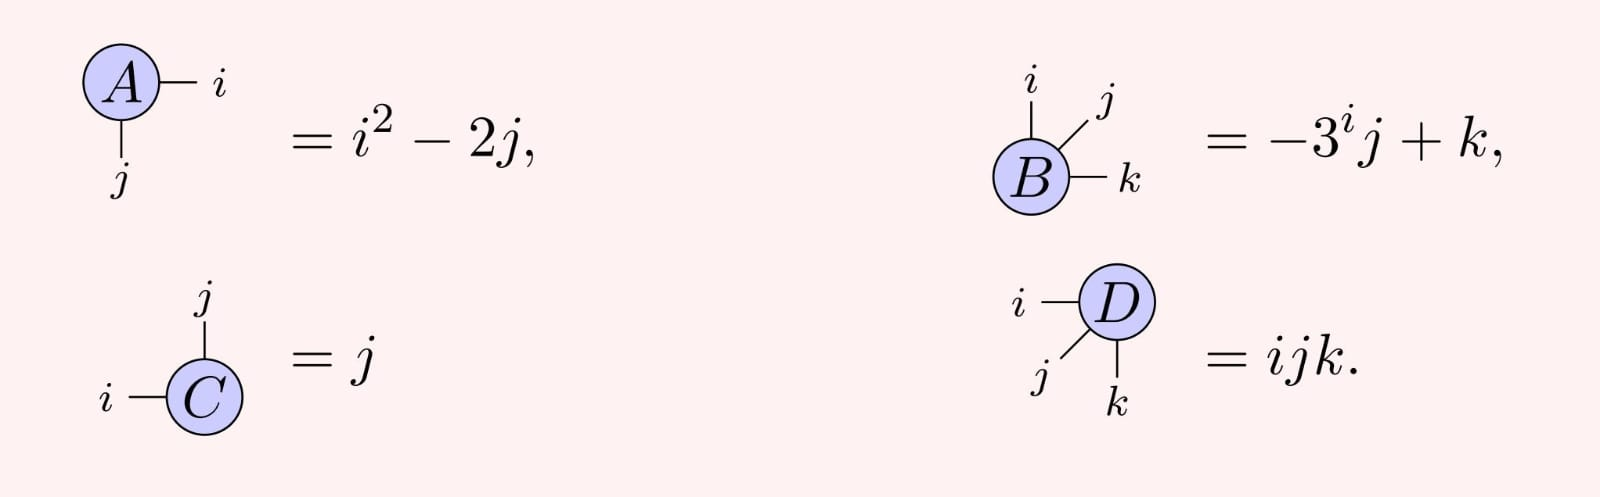
\includegraphics[width=0.6\linewidth]{images/tensorq1-1.jpeg}%
    \caption{Definitions of $A$, $B$, $C$ and $D$, Eqs.\eqref{def}}%
\end{figure}%

Calculate the value of the tensor network of Eq.~(1.22).

\begin{figure}[H]\centering
    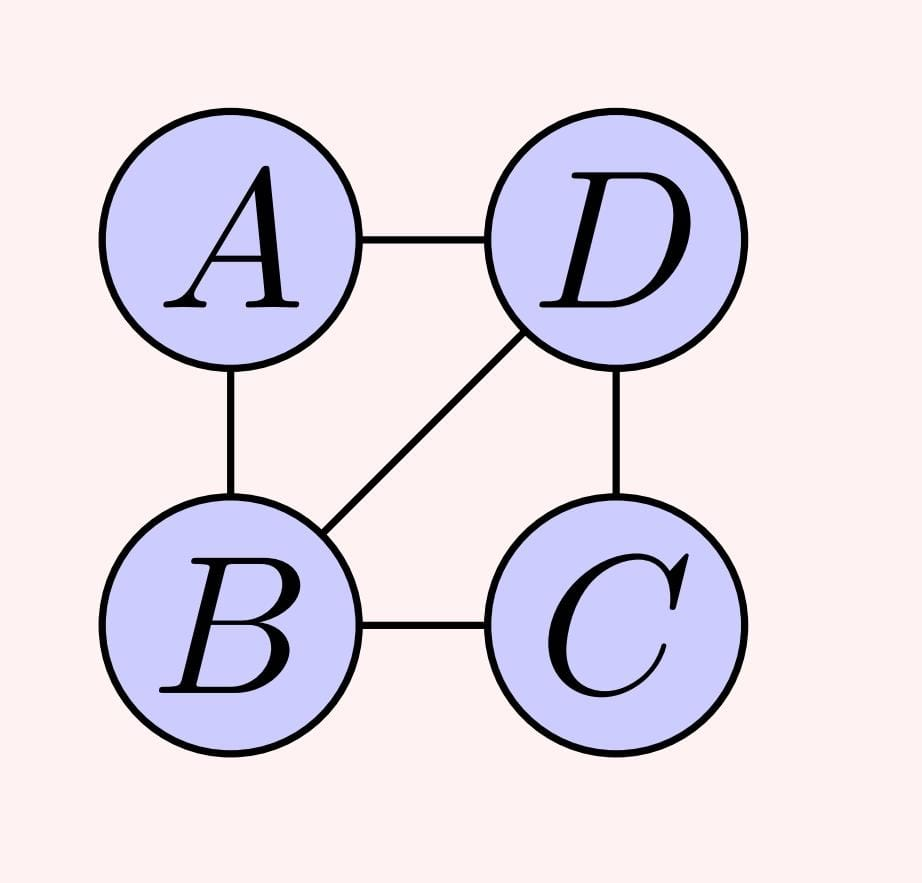
\includegraphics[width=0.25\linewidth]{images/tensorq1-2.jpeg}%
    \caption{The network to be contracted, Eq.~(1.22).}%
\end{figure}
\end{problem}


% ============================================================== solutions ===

\begin{solution}
There is no free index, so this is a scalar (the number of lines equal the number of indexed summed and must be consistent with the ordering $A_{i,j}, B_{i,j,k}$ to differentiate weach element of the tensor)
\begin{equation}
\begin{split}
     T &= \sum_{a,b,c,d,e} A_{a,b}B_{b,c,d}C_{d,e}D_{a,c,e}\\
     &= \sum_{a,b,c,d,e=0}^{2} (a^2  -2b)(-3^bc+d)(e)(ace)\\
     &= 1080
\end{split}
\end{equation}


\end{solution}


\attempt{
  date        = 2026-09-14,
  time        = 5min,
  difficulty  = 1,
  how it went = ,
}

\end{entry}
\begin{entry}{Q012}{Bubbling a network into a contraction table}

\entrymeta{
  topic   = {Tensor networks; contraction sequences; bubbling.},
  est     = $\sim$10 minutes,
  origin  = {Sourced. The original exercise; the worked example is reproduced so the
    required table format is unambiguous.},
  source  = {J.~C. Bridgeman and C.~T. Chubb, \emph{Hand-waving and Interpretive Dance:
    An Introductory Course on Tensor Networks}, J.~Phys.~A \textbf{50}, 223001 (2017),
    \href{https://arxiv.org/abs/1603.03039}{arXiv:1603.03039}, Section~1.6,
    Problem~2.},
  prereq  = {Section 1.4 (bubbling).},
  status  = open,
}

\begin{problem}
When a contraction is actually coded up, one contracts the tensors in one at a time and
must track, at each step, the open indices of the object built so far, the tensor being
absorbed, which indices are summed over in that step, and which new open indices the
incoming tensor contributes.

\begin{figure}[H]\centering
    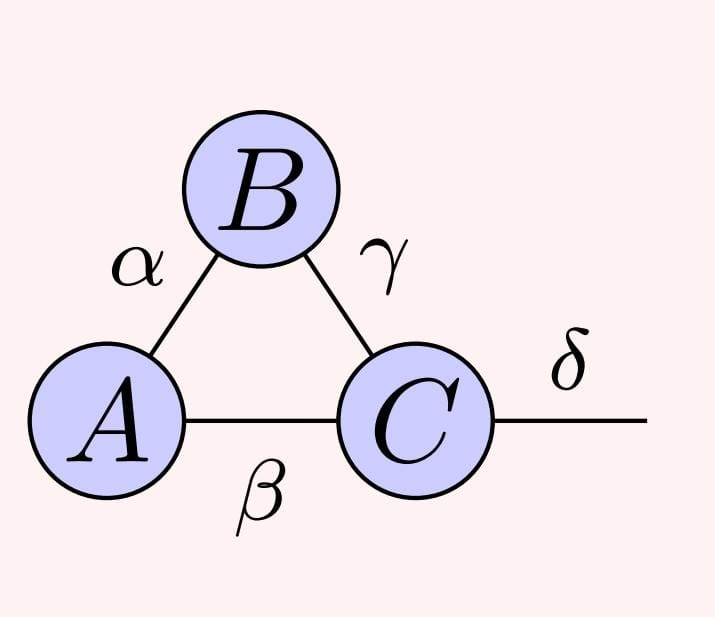
\includegraphics[width=0.2\linewidth]{images/tensorq2-1.jpeg}%
    \caption{The network of Eq.~(1.23), to be bubbled in alphabetical order.}%
\end{figure}


As an example, take the network of Eq.~(1.23): three tensors $A,B,C$ with bonds
$\alpha$ joining $A$ and $B$, $\beta$ joining $A$ and $C$, $\gamma$ joining $B$ and $C$,
and a free leg $\delta$ on $C$. Bubbling in alphabetical order gives


\begin{center}
\begin{tabular}{|c|c|c|c|}
\hline
Current & Tensor & Contract & New \\
\hline
--             & $A$ & --             & $\alpha,\beta$ \\
$\alpha,\beta$ & $B$ & $\alpha$       & $\gamma$ \\
$\beta,\gamma$ & $C$ & $\beta,\gamma$ & $\delta$ \\
\hline
\end{tabular}
\end{center}

Construct the corresponding table for the network of Eq.~(1.24), again bubbling in
alphabetical order.

\begin{figure}[H]\centering
    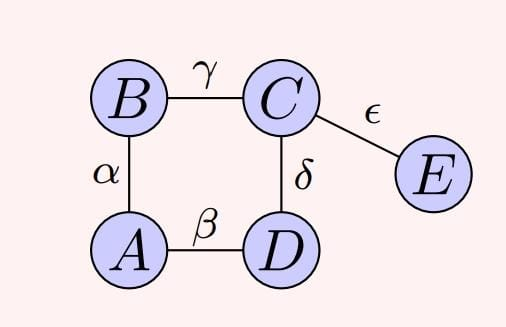
\includegraphics[width=0.2\linewidth]{images/tensorq2-2.jpeg}%
    \caption{The network of Eq.~(1.24), to be bubbled in alphabetical order}%
\end{figure}

and state the largest rank reached by the intermediate object, and whether a different
bubbling order would reduce it.

\end{problem}

% ============================================================== solutions ===

\begin{solution}
.
\vspace{0.1cm}
\begin{center}
\begin{tabular}{|c|c|c|c|}
\hline
Current & Tensor & Contract & New \\
\hline
--                      & $A$ & --          & $\alpha,\beta$ \\
  $\alpha,\beta$        & $B$ & $\alpha$    & $\gamma$   \\
 $\beta,\gamma$         & $C$ &  $\gamma$   &  $\delta,\epsilon$ \\
$\beta,\delta,\epsilon$ & $D$ &   $\delta,\beta$  & -- \\
            $\epsilon$  & $E$ &   $\epsilon$      &  -- \\
\hline
\end{tabular}
\end{center}
\vspace{0.1cm}
The largest rank is achieved after adding the tensor $C$ ($-A-B-C=$), where in this intermediate step we have a $\rank=3$ tensor. We could reduce the highest intermediate rank by starting from $E$, then going to $C$, we would contract $\epsilon$ and the intermediate tensor would be $\rank=2$, then, we can follow the adjacent $\rank=2$ tensors in the orders $B,A,D$ or $D,A,B$, on both cases at least one index is contracted and at most one is added, keeping the $\rank$ always lower or equal to $2$.
\end{solution}



\attempt{
  date        = 2026-09-14,
  time        = 10min,
  difficulty  = 1,
  how it went = ,
}

\end{entry}

\daysession{9}{2026-09-15}
\begin{entry}{Q013}{Counting colourings with tensor networks}

\entrymeta{
  topic   = {Tensor networks; graph colouring; counting complexity.},
  est     = $\sim$30 minutes total --- longer than the usual daily entry.
    Part (a) alone is $\sim$12 minutes and is the core; (b) and (c) may be done
    in a second sitting.,
  origin  = {Sourced. The original exercise; the definitions of $e$ and $n$ from
    Section~1.5 are inlined so the statement stands alone.},
  source  = {J.~C. Bridgeman and C.~T. Chubb, \emph{Hand-waving and Interpretive Dance:
    An Introductory Course on Tensor Networks}, J.~Phys.~A \textbf{50}, 223001 (2017),
    \href{https://arxiv.org/abs/1603.03039}{arXiv:1603.03039}, Section~1.6,
    Problem~3.},
  prereq  = {Section 1.5 (computational complexity).},
  status  = open,
}

\begin{problem}
Recall the two binary tensors of Section~1.5. The tensor $e$ takes the value $1$ if and
only if all of its indices are equal, and $0$ otherwise; the tensor $n$ takes the value
$1$ if and only if all of its indices differ, and $0$ otherwise. Given an arbitrary
graph, build a tensor network by placing an $e$ tensor at each vertex and an $n$ tensor
in the middle of each edge, inheriting the connectivity of the graph, as in
Eq.~(1.19).

\begin{figure}[H]\centering
    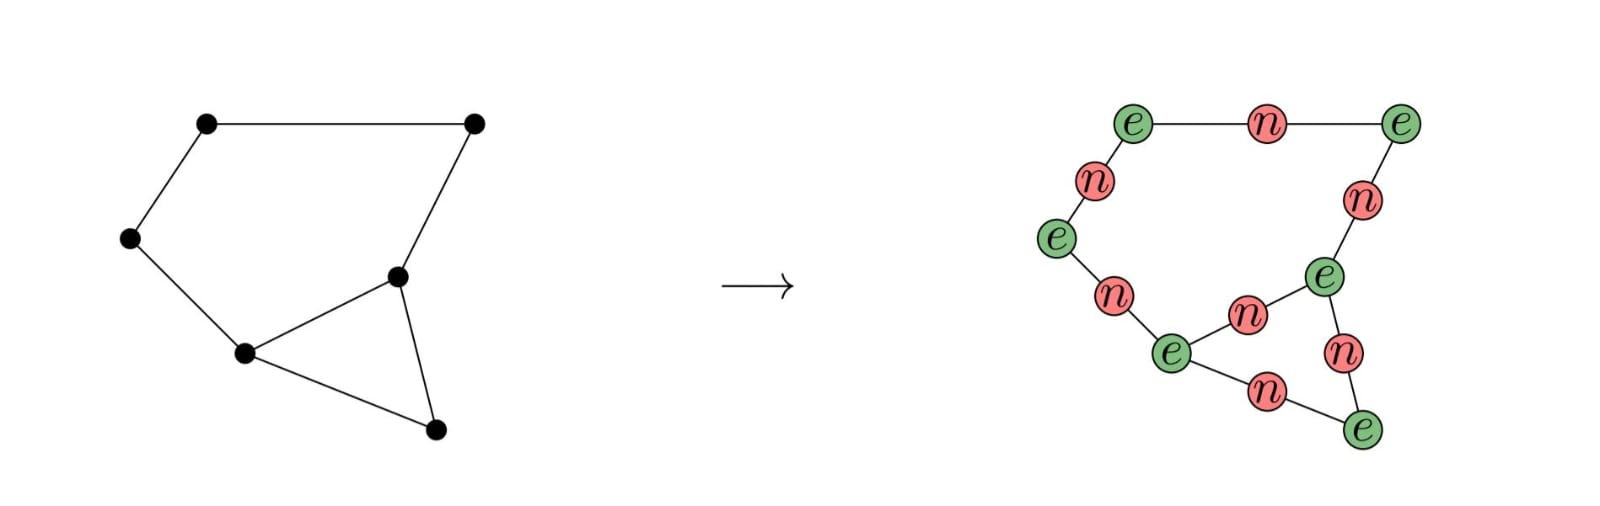
\includegraphics[width=0.7\linewidth]{images/tensorq3-1.jpeg}%
    \caption{The graph of Eq.~(1.19) and the tensor network built from it.}%
\end{figure}%

With $q$-dimensional indices, the nonzero contributions to this network are exactly the
vertex $q$-colourings of the graph, so its contraction counts them.

\begin{enumerate}[label=\textbf{(\alph*)},leftmargin=*]
  \item Calculate the contraction of the network of Eq.~(1.19) for bond dimension $q$,
        i.e.\ the number of three-colourings of the corresponding graph.
  \item Using the $e$ and $n$ tensors, construct a tensor network whose contraction gives
        the number of \emph{edge} colourings. For a planar graph, construct an analogous
        network counting \emph{face} colourings.
\end{enumerate}


\end{problem}

% ============================================================== solutions ===

\begin{solution}[Part (a)]
The equivalent tensor of e connected to two n, is
\begin{equation}
\begin{split}
    x_{a,b} &= \sum_{i,j}n_{a,i}e_{i,j}n_{j,b}\\
    &= \sum_{i,j} (1-\delta_{a,i})\delta_{i,j}(1-\delta_{j,b})\\
    &= \sum_{i} (1-\delta_{a,i})(1-\delta_{i,b})\\
    &= \delta_{a,b} + (q-2)
\end{split} 
\end{equation}

% requires \usepackage{tikz}
\usetikzlibrary{fit}
% requires \usetikzlibrary{fit}
\begin{figure}[H]\centering
\resizebox{\linewidth}{!}{%
\begin{tikzpicture}[
  every node/.style={font=\footnotesize},
  ten/.style={circle,draw,minimum size=5.5mm,inner sep=0pt},
  blu/.style={ten,fill=blue!20},
  red/.style={ten,fill=red!35},
  yel/.style={ten,fill=yellow!55},
  grn/.style={ten,fill=green!35},
  cut/.style={draw,dashed,thick,rounded corners,inner sep=3pt},
]

%=================== PANEL 1 : original, relaid out ===================
\begin{scope}[shift={(0,0)}]
  % upper branch: v5 - v3 - v1 - v2 - v4
  \node[blu] (v1) at (2.0, 2.6) {$e$};
  \node[blu] (nb) at (1.2, 2.3) {$n$};
  \node[blu] (v3) at (0.4, 2.0) {$e$};
  \node[blu] (nc) at (0.2, 1.0) {$n$};
  \node[blu] (na) at (2.8, 2.3) {$n$};
  \node[blu] (v2) at (3.6, 2.0) {$e$};
  \node[blu] (nd) at (3.8, 1.0) {$n$};
  % axis
  \node[blu] (v5) at (0.0, 0.0) {$e$};
  \node[blu] (nn) at (2.0, 0.0) {$n$};
  \node[blu] (v4) at (4.0, 0.0) {$e$};
  % lower branch: v5 - v6 - v4
  \node[blu] (nf) at (1.2,-1.5) {$n$};
  \node[blu] (v6) at (2.0,-1.9) {$e$};
  \node[blu] (ng) at (2.8,-1.5) {$n$};

  \draw (v5)--(nc)--(v3)--(nb)--(v1)--(na)--(v2)--(nd)--(v4);
  \draw (v5)--(nn)--(v4);
  \draw (v5) to[bend right=12] (nf);
  \draw (nf)--(v6)--(ng);
  \draw (ng) to[bend right=12] (v4);

  \node[cut,red!80!black,fit=(nc)(v3)(nb)] {};
  \node[cut,red!80!black,fit=(na)(v2)(nd)] {};
  \node[cut,red!80!black,fit=(nf)(v6)(ng)] {};
\end{scope}

\node at (5.1,0.3) {\Large$\to$};

%=================== PANEL 2 : after x-reduction ===================
\begin{scope}[shift={(6.0,0)}]
  \node[blu] (w1) at (2.0, 2.3) {$e$};
  \node[red] (x2) at (0.7, 1.5) {$x$};
  \node[red] (x1) at (3.3, 1.5) {$x$};
  \node[blu] (w5) at (0.0, 0.0) {$e$};
  \node[blu] (nn) at (2.0, 0.0) {$n$};
  \node[blu] (w4) at (4.0, 0.0) {$e$};
  \node[red] (x3) at (2.0,-1.5) {$x$};

  \draw (w5)--(x2)--(w1)--(x1)--(w4);
  \draw (w5)--(nn)--(w4);
  \draw (w5) to[bend right=15] (x3);
  \draw (x3) to[bend right=15] (w4);

  \node[cut,yellow!60!black,fit=(x2)(w1)(x1)] {};
  \node[cut,green!50!black,fit=(w5)(nn)(x3)(w4)] {};
\end{scope}

\node at (11.1,0.3) {\Large$\to$};

%=================== PANEL 3 : y over z ===================
\begin{scope}[shift={(11.9,0)}]
  \node[yel] (y) at (0.9, 1.3) {$y$};
  \node[grn] (z) at (0.9,-0.6) {$z$};
  \draw (y) to[bend left=38]  (z);
  \draw (y) to[bend right=38] (z);
  \node[cut,gray,fit=(y)(z)] {};
\end{scope}

\node at (13.9,0.3) {\Large$\to$};

%=================== PANEL 4 : scalar ===================
\begin{scope}[shift={(14.5,0)}]
  \node[ten,fill=gray!40] at (0.5,0.3) {};
\end{scope}

\end{tikzpicture}}
\caption{Contraction of the network of Eq.~(1.19), redrawn so that the three
$n$--$e$--$n$ chains occupy disjoint regions. Red contours mark the chains replaced by
$x$; the yellow contour is $x$--$e$--$x\to y$; the green contour is the pair of vertices
joined by the parallel $n$ and $x$ bonds, $\to z$. Contracting $y$ against $z$ across the
double bond leaves a scalar.}
\end{figure}%

The upper part inside the yellow dashed line is equivalent to 
\begin{equation}
\begin{split}
    y_{a,b}&= \sum_{i,j}x_{a,i}e_{i,j}x_{j,b}\\
    &=\sum_{i,j} x_{a,i}\delta_{i,j}x_{j,b}\\
    &= \sum_{i} x_{a,i}x_{i,b}\\
    &= \sum_i (q-2)^2 + (q-2)(\delta_{a,i}+\delta_{i,b}) + \delta_{a,i}\delta_{i,b}\\
    &= q(q-2)^2+ 2(q-2) + \delta_{a,b}
\end{split}
\end{equation}
whereas for the below part inside the green dashed line is equivalent to 

\begin{equation}
\begin{split}
    z_{a,b}&= \sum_{i,j,k,l}e_{a,i,j}x_{j,l}n_{i,k}e_{k,l,b}\\
    &=\sum_{i,j,k,l}\delta_{a,i,j}x_{j,l}n_{i,k}\delta_{k,l,b}\\
    &= x_{a,b}n_{a,b}
\end{split}
\end{equation}
so
\begin{equation}
\begin{split}
    T&=\sum_{a,b} z_{a,b}y_{a,b}\\
    &= \sum_{a,b} (q(q-2)^2+ 2(q-2) + \delta_{a,b})((q-2)+\delta_{a,b})(1-\delta_{a,b})\\
    &= q(q-1)(q-2)^2[q^2-2q+2]
\end{split}
\end{equation}


\end{solution}

\begin{solution}[Part (b)]
These tensor $e$ and $n$ allows one to generalize the q-colouring counting problem by simple using $e$ in place of the counting object and $n$ used as the "adjacency mediator"  forcing that no adjacent objects have the same colour. To count the number of edges colouring you may draw a tensor network with $e$ in the edges and $n$ in the vertices, meanwhile to count the number of face colouring you draw a network with $e$ in the face( inside each polygon) and $n$ in the commom edges of the polygons. 
\end{solution}





\attempt{
  date        = ,
  time        = ,
  difficulty  = ,
  how it went = ,
}

\end{entry}

\daysession{10}{2026-09-17}
\begin{entry}{Q014}{Grassmann integrals and the trace of a Floquet operator}

\entrymeta{
  topic   = {Grassmann (Berezin) integration; Gaussian fermionic integrals;
    field-theory approach to quantum chaos.},
  est     = $\sim$25 minutes --- longer than the usual daily entry; part (c) is the core
    and may be done separately.,
  origin  = {Adapted. Reconstructed from a lecture exercise; the Grassmann axioms are
    inlined and the time-lattice conventions fixed so the statement is self-contained.},
  source  = {T. Micklitz, lectures on \emph{Field-Theory Approach to Quantum Chaos},
    School on Analytical and Numerical Methods for Disordered Quantum Systems.},
  prereq  = {None beyond linear algebra; all Grassmann conventions are stated below.},
  status  = open,
}

\begin{problem}
\textbf{Conventions.} Let $\psi_1,\dots,\psi_n,\bar\psi_1,\dots,\bar\psi_n$ be
\emph{Grassmann variables}: generators of an associative algebra over $\CC$ subject to
\[
  \{\psi_i,\psi_j\}=\{\bar\psi_i,\bar\psi_j\}=\{\psi_i,\bar\psi_j\}=0
  \qquad\text{for all } i,j,
\]
so in particular $\psi_i^{2}=\bar\psi_i^{2}=0$. Every function of them is a polynomial
of degree at most one in each generator. \emph{Berezin integration} in a single variable
is the linear map defined by
\begin{equation}
    \int d\psi\;1=0,
  \qquad
  \int d\psi\;\psi=1,
  \label{grassman identity}
\end{equation}

and the differentials $d\psi_i,d\bar\psi_i$ anticommute with each other and with all
generators. For $n$ pairs write
\[
  D(\bar\psi,\psi):=\prod_{i=1}^{n} d\bar\psi_i\, d\psi_i ,
  \qquad\text{normalised so that}\qquad
  \int D(\bar\psi,\psi)\;\prod_{i=1}^{n}\psi_i\bar\psi_i \;=\;1 .
\]
For $A\in\CC^{n\times n}$ set $\bar\psi A\psi:=\sum_{i,j}\bar\psi_i A_{ij}\psi_j$.

\begin{enumerate}[label=\textbf{(\alph*)},leftmargin=*]
  \item Prove that
        \[
          \int D(\bar\psi,\psi)\; e^{-\bar\psi A\psi} \;=\;\det A .
        \]
  \item Prove that, for $A$ invertible,
        \[
          \int D(\bar\psi,\psi)\; e^{-\bar\psi A\psi}\,\psi_a\bar\psi_b
          \;=\;\det A\;\bigl(A^{-1}\bigr)_{ab} .
        \]
  \item Let $U_0$ be a unitary on $\CC^{N}$ (one step of a Floquet evolution), and let
        the discrete time lattice be $\{0,1,\dots,t\}$, on which the lowering operator
        $T_-$ acts by $T_-\ket{\tau}=\ket{\tau-1}$, i.e.
        $(T_-)_{\tau,\tau'}=\delta_{\tau,\tau'-1}$. Take Grassmann variables
        $\psi_{(i,\tau)},\bar\psi_{(i,\tau)}$ indexed by $i\in\{1,\dots,N\}$ and
        $\tau\in\{0,\dots,t\}$, and set
        \[
          A=\id-U_0\otimes T_- .
        \]
        Show that $\det A=1$, compute $\bigl(A^{-1}\bigr)_{(i,\tau),(j,\tau')}$, and
        conclude that
        \[
          \int D(\bar\psi,\psi)\; e^{-\bar\psi A\psi}
          \sum_{a=1}^{N}\psi_{(a,0)}\,\bar\psi_{(a,t)}
          \;=\;\Tr\bigl(U_0^{\,t}\bigr).
        \]
        Explain why an insertion diagonal in the time index, $\sum_a
        \psi_{(a,\tau)}\bar\psi_{(a,\tau)}$, cannot produce this result.
\end{enumerate}
\end{problem}

% ============================================================== solutions ===

\begin{solution}[Part (a)]
Since $\psi_i^{2}=\bar\psi_i^{2}=0$, we have that 
\begin{equation}
    e^{-\bar\psi A\psi}= \prod_{i,j}(1 -  \bar\psi_i A_{ij}\psi_j)=O(0)+O(2)+...+O(2n)
\end{equation}
where here $O(2k)$ represent the term where there is a product of $2k$ Grassmann variables, i.e.,
\begin{equation*}
\begin{split}
    O(2k)= (-1)^k\sum_{\substack{i_1\neq...\neq i_k\\j_1\neq...\neq j_k}} \prod_{x=1}^{k}\bar\psi_{i_x}A_{i_x,j_x}\psi_{j_x}
\end{split}
\end{equation*}
(notice that equal index leads to 0 contribution, $\psi_i^{2}=\bar\psi_i^{2}=0$ forcing the summation to be over different index) but from \eqref{grassman identity}, any term that doesn't have the full $2n$ Grassmann variables vanishes when integrated, $\int D(\bar\psi,\psi) O(2k)=0,\ k<n$, then 
\begin{equation}
\begin{split}
    \int D(\bar\psi,\psi)\; e^{-\bar\psi A\psi} = \int D(\bar\psi,\psi) \sum_{\substack{i_1\neq...\neq i_n\\j_1\neq...\neq j_n}} \prod_{x=1}^{n}\bar\psi_{i_x}A_{i_x,j_x}\psi_{j_x}
\end{split}
\end{equation}
which can be rewritten in the permutation notation 
\begin{equation}
\begin{split}
    \int D(\bar\psi,\psi)\; e^{-\bar\psi A\psi} =& (-1)^n\int D(\bar\psi,\psi) \sum_{\sigma \in S_n} \prod_i^n \bar\psi_i A_{i\sigma(i)}\psi_{\sigma(i)}\\
    =& (-1)^n\sum_{\sigma \in S_n}\int D(\bar\psi,\psi)\prod_i\bar\psi_i \psi_{\sigma(i)}A_{i \sigma(i)}.
\end{split}
\end{equation}
Now, due to the anti-commutativity of the Grassmann variables, we can rewrite the normalization condition and then derive for a generic permutation
\begin{equation}
   \int D(\bar\psi,\psi)\prod_i\bar\psi_i \psi_{i} =(-1)^n\implies\int D(\bar\psi,\psi)\prod_i\bar\psi_i \psi_{\sigma(i)}=(-1)^n\text{sign}(\sigma)
\end{equation}, where an even permutation would require an even number of exchanges to order the integral as products $\int d \psi \psi$, meanwhile an odd permutation requires an odd number of exchanges, leading to a $-$ sign overall, hence
\begin{equation}
\begin{split}
    \int D(\bar\psi,\psi)\; e^{-\bar\psi A\psi}
    =&\sum_{\sigma \in S_n}\text{sign}(\sigma)\prod_iA_{i \sigma(i)}\\
    =& \det (A
)\end{split}
\end{equation}
\end{solution}

\begin{solution}[Part (b)]
We can see the matrix itself as a list of complex variables, consider Einstein summation notation for an Euclidean norm, such that the expression can be written as (for the sake of precision consider $X_{i,j}$ the list of complex variables)
\begin{equation}
\begin{split}
    \int D(\bar\psi,\psi)\; e^{-\bar\psi A\psi}\psi_a \bar\psi_b
    =&\int D(\bar\psi,\psi)\; e^{-\bar\psi^\nu A_{\nu\mu}\psi^\mu}\psi_a \bar\psi_b\\
    =& \int D(\bar\psi,\psi)\; e^{-\bar\psi^\nu A_{\nu\mu}\psi^\mu}(-\bar\psi_b \psi_a) \\
    =&\bigg(\frac{\partial}{\partial X_{ba}}\int D(\bar\psi,\psi)\; e^{-\bar\psi^\nu X_{\nu\mu}\psi^\mu}\bigg)_{X=A}\\
    =& \bigg(\frac{\partial}{\partial X_{ba}}\det(X)\bigg)_{X=A}
\end{split}
\end{equation}
From Cramer's rule for the determinant, for any row $i$
\begin{equation*}
    \det X = \sum_{j}X_{ij}C_{ij}
\end{equation*}
where $C_{ij}$ is the cofactor in the corresponding position $i,j$, which depends on all variables of $X$ besides the ones that have either row $i$ or column $j$ (you eliminate the row $i$ and columns $j$ to calculate the determinant of the remaining matrix, to attain $C_{i,j}$), so taking the row $i=b$, we can write $\det X = \sum_{j}X_{bj}C_{bj}$. No element of the summation depends on $X_{ba}$ besides when $j=a$, so
\begin{equation*}
    \frac{\partial}{\partial X_{ba}}\det X = C_{ba}
\end{equation*}
Now, from Laplace's formula for the inverse, or cofactor method, the inverse is calculated precisely from the cofactor by
$$(X^{-1})_{ij} =\frac{C_{ji} }{\det X}$$
therefore
\begin{equation}
    \int D(\bar\psi,\psi)\; e^{-\bar\psi A\psi}\psi_a \bar\psi_b
    = \det A (A^{-1})_{ab}
\end{equation}
\end{solution}

\begin{solution}[Part (c)]
Defining properly the notation for the spatial and temporal degrees of freedom
\begin{equation}
\begin{split}
    \sum_{a,a',\tau,\tau'} \bar \psi_{(a,\tau)} (U^k_0\otimes T_-^k)_{(a,a'),(\tau,\tau')} \psi_{(a',\tau')}= \sum_{a,a',\tau,\tau'} \bar \psi_{(a,\tau)} (U^k_0)_{(a,a')}\otimes (T_-^k)_{(\tau,\tau')} \psi_{(a',\tau')}
\end{split}
\end{equation}
Now notice 
\begin{equation}
    T_-=\sum_{\tau=1}^{t}\ket{\tau-1}\bra{\tau}
=\begin{pmatrix}
0 & 1 & 0 & \cdots & 0 \\
0 & 0 & 1 & \ddots & \vdots \\
\vdots & \vdots & \ddots & \ddots & 0 \\
0 & 0 & \cdots & 0 & 1 \\
0 & 0 & \cdots & 0 & 0 \qquad 
\end{pmatrix},
\qquad
(T_-)_{\tau\tau'}=\delta_{\tau,\tau'-1}. \qquad \text{odering}\ \ket{0} = \begin{pmatrix}
    1\\
    ...\\
    0
\end{pmatrix}
\end{equation}
exponentiation of $T_-$ lower its own entries, leading to
\begin{equation}
T_-^{\,k}=\sum_{\tau=1}^{t}\ket{\tau-1}\bra{\tau}
=\begin{pmatrix}
0_{(t+1-k)\times k} & \id_{t+1-k} \\[2pt]
0_{k\times k} & 0_{k\times(t+1-k)}
\end{pmatrix},
\quad (T_-^{\,k})_{\tau\tau'}=\delta_{\tau,\tau'-k},,
\qquad T_-^{\,t+1}=0 ,
\end{equation}
Moreover, we have that $(T_-^k)_{0t} = \delta_{kt}$, which means that the we got apply the $T_-$ $t$ times in order to have an element in the last columns of the first row, meanwhile the condition $T_{-}^{t+1}=0$, makes $U_0\otimes T_-$ nilpotent, such that the inverse of $A=\id-U_0\otimes T_-$ can be calculated from the geometric series, 
\begin{equation}
    (\id -U_0\otimes T_-)^{-1}= \sum_{k=0}^t U_0^k \otimes T_{-}^k
\end{equation}
 thus
\begin{equation}
    (A^{-1})_{(a,0),(b,t)}= (U_0^t)_{a,b}
\end{equation}
Finally,
\begin{equation}
    A=\id-U_0\otimes T_-=
\begin{pmatrix}
\id_N & -U_0 & & & \\
 & \id_N & -U_0 & & \\
 & & \ddots & \ddots & \\
 & & & \id_N & -U_0 \\
 & & & & \id_N
\end{pmatrix}
\end{equation} such that $\det A=1$, therefore, using item b) 
\begin{equation}
    \int D(\bar\psi,\psi)\; e^{-\bar\psi A\psi}
          \sum_{a=1}^{N}\psi_{(a,0)}\,\bar\psi_{(a,t)}
          \;=\; \sum_a =\Tr\bigl(U_0^{\,t}\bigr).
\end{equation}
 



\end{solution}



\attempt{
  date        = 2026-09-15,
  time        = ,
  difficulty  = ,
  how it went = ,
}

\end{entry}
\begin{entry}{Q015}{From free to damped: the arc propagator at finite $\gamma$}

\entrymeta{
  topic   = {Discrete-time field theory; contour times; finite-difference Green
    functions; quantum chaos.},
  est     = $\sim$15 minutes,
  origin  = {Adapted. Reconstructed from a lecture exercise; the index conventions,
    the Heaviside convention and the structural part (a) are inlined so the statement
    stands alone.},
  source  = {T. Micklitz, lectures on \emph{Field-Theory Approach to Quantum Chaos},
    School on Analytical and Numerical Methods for Disordered Quantum Systems.
    Companion to \qref{Q016}.},
  prereq  = {None beyond finite differences.},
  status  = open,
}

\begin{problem}
\textbf{What this describes.} In the field theory of the previous entry, the object of
interest is not a single amplitude but a \emph{pair} of them: one propagating forward in
time and one backward, whose phases cancel and which therefore survive an average over
the random dynamics. The propagator $\Pi$ follows such a pair, and each of its legs
carries two times, one on each branch. The free theory has no scale: once formed, a pair
stays correlated forever. The interacting theory has one, $\gamma$, at which the two
branches lose their correlation; the exercise is to see that scale appear, and to see
what it means.

\textbf{Conventions.} Time is discrete, $n\in\ZZ$. Each leg carries a pair of contour
times $(n^{+},n^{-})$, forward and backward. Write the pair as a single label,
\[
  \mathbf n:=(n^{+},n^{-}),
  \qquad
  \Delta n:=n^{+}-n^{-}\ \ \text{(relative time)},
  \qquad
  \bar n:=\tfrac12\bigl(n^{+}+n^{-}\bigr)\ \ \text{(mean time)} ,
\]
so that $\mathbf n\mapsto(\Delta n,\bar n)$ is a change of coordinates on the set of
pairs: $\Delta n$ records how far apart on the two branches the pair sits, and $\bar n$
how far along both have travelled together.

The propagator $\Pi_{\mathbf n_2,\mathbf n_1}$ is a kernel from the incoming pair
$\mathbf n_1$ to the outgoing pair $\mathbf n_2$. Kernels compose by summation over the
repeated pair,
\[
  (KL)_{\mathbf n_2,\mathbf n_1}
  :=\sum_{\mathbf m}K_{\mathbf n_2,\mathbf m}\,L_{\mathbf m,\mathbf n_1},
  \qquad
  \bigl(\id\bigr)_{\mathbf n_2,\mathbf n_1}
  =\delta_{n_2^{+},n_1^{+}}\,\delta_{n_2^{-},n_1^{-}} ,
\]
and act on the outgoing label only. Let $T$ be the kernel that advances \emph{both}
contour times by one unit --- one step of the dynamics, applied to both branches at
once,
\[
  T_{\mathbf n,\mathbf m}
  :=\delta_{n^{+},\,m^{+}+1}\;\delta_{n^{-},\,m^{-}+1},
\]
and set $d:=\id-T$, the discrete counterpart of a time derivative. Write $\Theta(u)=1$
for $u\ge0$ and $\Theta(u)=0$ for $u<0$, so that $\Pi$ is supported on outgoing times
later than incoming ones. Finally let $D_0>0$ be the normalisation constant of the notes
and $\gamma>0$ a damping rate.

\begin{enumerate}[label=\textbf{(\alph*)},leftmargin=*]
  \item Show that $T$ preserves the relative time and lowers the mean time by one:
        in the coordinates $(\Delta n,\bar n)$,
        \[
          T_{\mathbf n,\mathbf m}
          =\delta_{\Delta n,\Delta m}\;\delta_{\bar n,\,\bar m-1}.
        \]
        Deduce that if $K_{\mathbf n_2,\mathbf n_1}
        =\delta_{\Delta n_2,\Delta n_1}\,f(\bar n_2-\bar n_1)$ for some
        $f:\ZZ\to\CC$, then
        \[
          (dK)_{\mathbf n_2,\mathbf n_1}
          =\delta_{\Delta n_2,\Delta n_1}\bigl[f(u)-f(u-1)\bigr],
          \qquad u:=\bar n_2-\bar n_1 ,
        \]
        so that the problem reduces to a one-dimensional recursion in $u$.

  \item \emph{Free theory.} Verify that the propagator for the free theory
        \[
          \Pi_{\mathbf n_2,\mathbf n_1}
          =\frac{1}{D_0}\,\delta_{\Delta n_2,\Delta n_1}\,\Theta(\bar n_2-\bar n_1)
        \]
        satisfies
        \[
          (d\,\Pi)_{\mathbf n_2,\mathbf n_1}
          =\frac{1}{D_0}\,\delta_{\Delta n_2,\Delta n_1}\,
            \delta_{\bar n_2,\bar n_1} .
        \]

  \item \emph{Interacting theory.} The propagator for the interacting theory (with mass) is
        \[
          \Pi^{\mathrm{arc}}_{\mathbf n_2,\mathbf n_1}
          =\frac{1}{D_0}\,\delta_{\Delta n_2,\Delta n_1}\,
            \frac{\Theta(\bar n_2-\bar n_1)}{(1+\gamma)^{\,\bar n_2-\bar n_1+1}} .
        \]
        Show that 
        \[
          \bigl[(d+\gamma)\,\Pi^{\mathrm{arc}}\bigr]_{\mathbf n_2,\mathbf n_1}
          =\frac{1}{D_0}\,\delta_{\Delta n_2,\Delta n_1}\,
            \delta_{\bar n_2,\bar n_1} ,
        \]
        i.e.\ $\Pi^{\mathrm{arc}}$ is the Green function of $d+\gamma$ with the same
        right-hand side as in the free case. Note where the factor
        $(1+\gamma)^{-u}$ disappears from the final answer.

   \item \emph{The lattice scale.} Fix the relative time and compare successive mean
        times: show that for $\bar n_2\ge\bar n_1$ the ratio
        \[
          \frac{\Pi^{\mathrm{arc}}_{\,(\Delta n,\,\bar n_2+1),\,\mathbf n_1}}
               {\Pi^{\mathrm{arc}}_{\,(\Delta n,\,\bar n_2),\,\mathbf n_1}}
        \]
        does not depend on $\bar n_2$, and identify it. The decay is therefore
        geometric: the same fraction of the amplitude is lost at every step, regardless
        of how long the pair has already survived.

        Explain why this is the expected structure rather than a coincidence, by reading
        it off the equation $\Pi^{\mathrm{arc}}=\bigl[(1+\gamma)\id-T\bigr]^{-1}$ that
        (c) establishes: each application of $T$ advances both branches by one step of
        the dynamics, and each such step is accompanied by the same factor. What
        property of the underlying dynamics does this memorylessness reflect, and what
        would have to change for the loss per step to depend on $\bar n_2-\bar n_1$?


  \item \emph{The approximation.} Show that $(1+\gamma)^{-u}=e^{-\gamma u}$ up to a
        relative error controlled by $\gamma^{2}u$, and say why it is this product,
        rather than $\gamma$ alone, that must be small for the exponential form to hold. Determine also the sign of
        the discrepancy: does the lattice decay faster or slower than the exponential?

  \item \emph{The continuum limit.} Take as given that the Green function of
        $\partial_{\mathcal T}+\Gamma$ is $\Theta(\mathcal T)\,e^{-\Gamma\mathcal T}$,
        where the constant $\Gamma$ added to a first-order derivative is a \emph{mass
        term} and fixes the only scale of the continuum theory, $\tau=1/\Gamma$. Let
        $\delta t$ be the physical duration of one lattice step, so that
        $\mathcal T=u\,\delta t$ and $\gamma=\Gamma\,\delta t$. Using~(e), show that
        $\Pi^{\mathrm{arc}}$ converges to the continuum Green function as
        $\delta t\to0$, and state precisely which quantity is held fixed in the limit
        and which is sent to zero. Explain why the limit cannot be taken at fixed $u$,
        nor at fixed $\gamma$, and why the physically meaningful statement is that
        $\delta t$ disappears from the answer while $\tau$ does not: the scale belongs
        to the theory, the lattice spacing to its description. How many lattice steps
        does one lifetime $\tau$ contain, and what does that number have to be for the
        continuum description to apply?
\end{enumerate}
\end{problem}

% ============================================================== solutions ===

\begin{solution}[a]
$n^+=m^+ - 1$ and $n^-=m^- - 1$ if and only if $n^+ - n^- = m^+ - m^-$ and $\frac{n^+ + n^-}{2} =\frac{m^+ + m^-}{2} -1$, thus
\[
          T_{\mathbf n,\mathbf m}
          =\delta_{\Delta n,\Delta m}\;\delta_{\bar n,\,\bar m+1}.
        \]
Applying $T$ to such $K$
\begin{equation}
    \begin{split}
        (TK)_{\mathbf n_2, \mathbf n_1} &= \sum_{\mathbf m} T_{\mathbf n_2,\mathbf{ m}}K_{\mathbf{ m}, \mathbf n_1}\\
        &= \sum_{\Delta m, \bar m} \delta_{\Delta n_2,\Delta m}\;\delta_{\bar n_2,\,\bar m+1} \delta_{\Delta m,\Delta n_1}\,f(\bar m - \bar n_1) \\
        &=  \delta_{\Delta n_2,\Delta n_1}f(\bar n_2 -1 -n_1)\\
        &=  \delta_{\Delta n_2,\Delta n_1}f(u-1)
    \end{split}
\end{equation}
Therefore, it follows directly when applying $d$

\end{solution}

\begin{solution}[b]
From a)
\begin{equation}
   (d\,\Pi)_{\mathbf n_2,\mathbf n_1}
          =\frac{1}{D_0}\,\delta_{\Delta n_2,\Delta n_1}\,
            \big(\Theta({\bar n_2-\bar n_1}) - \Theta({\bar n_2-\bar n_1}-1)\big)
\end{equation}
Now if $\bar n_2-\bar n_1-1 \geq 0$, both $\Theta$ are equal to 1, leading to a null for the finite difference. If $\bar n_2-\bar n_1<0$, both vanish. So the finite difference only survives when $\bar n_2-\bar n_1 = 0$. Therefore,
\[
          (d\,\Pi)_{\mathbf n_2,\mathbf n_1}
          =\frac{1}{D_0}\,\delta_{\Delta n_2,\Delta n_1}\,
            \delta_{\bar n_2,\bar n_1} .
        \]
\end{solution}

\begin{solution}[c]
Applying item a) we get that 
\begin{equation}
  d \Pi^{\mathrm{arc}}_{\mathbf n_2,\mathbf n_1}
          =\frac{1}{D_0}\,\delta_{\Delta n_2,\Delta n_1}\,
            \left(\frac{\Theta(\bar n_2-\bar n_1)}{(1+\gamma)^{\,\bar n_2-\bar n_1+1}}-\frac{\Theta(\bar n_2-\bar n_1-1)}{(1+\gamma)^{\,\bar n_2-\bar n_1}} \right) .
\end{equation}
Meanwhile 
\begin{equation}
\begin{split}
    \gamma \Pi^{\mathrm{arc}}_{\mathbf n_2,\mathbf n_1}
          &=\frac{1}{D_0}\,\delta_{\Delta n_2,\Delta n_1}\,
            \frac{\Theta(\bar n_2-\bar n_1)}{(1+\gamma)^{\,\bar n_2-\bar n_1}}\left(\frac{\gamma}{1+\gamma} \right) \\
         &=\frac{1}{D_0}\,\delta_{\Delta n_2,\Delta n_1}\,
            \frac{\Theta(\bar n_2-\bar n_1)}{(1+\gamma)^{\,\bar n_2-\bar n_1}}\left(1-\frac{1}{1+\gamma} \right)  
\end{split}
\end{equation}
 To conclude, we must notice that after summing both expressions, the delta makes the only non-zero contribution occur when $\bar n_2 = \bar n_1$, reducing the exponent of the denominator to 0
 \begin{equation}
 \begin{split}
      (d+\gamma) \Pi^{\mathrm{arc}}_{\mathbf n_2,\mathbf n_1}
          &=\frac{1}{D_0}\,\delta_{\Delta n_2,\Delta n_1}\,
            \frac{\delta_{\bar n_2,\bar n_1}}{(1+\gamma)^{\,\bar n_2-\bar n_1}} \\
            &= \frac{1}{D_0}\,\delta_{\Delta n_2,\Delta n_1}\,
            \delta_{\bar n_2,\bar n_1} 
 \end{split}
 \end{equation}
This can be seen as the mass term for the theory
\end{solution}

\begin{solution}[d]
The ratio is given by 
\begin{equation*}
        (1+\gamma)^{-1}
\end{equation*}
which is smaller than $1$, reflecting the expected damping.
Inverting the expression for item c) (the right-hand side can be seen as proportional to the identity) and applying the geometric series, which converges even we stop looking at finite time since $(1+\gamma)^{-1} <1$ for $\gamma>0$. 

\begin{equation}
\begin{split}
    \Pi^{\text{arc}}=&\frac{1}{D_0} \bigl[(1+\gamma)\id-T\bigr]^{-1}\\
    =& \frac{1}{D_0 (1+\gamma)} \bigl[\id- \frac{1}{(1+\gamma)}T\bigr]^{-1}\\
    =& \frac{1}{D_0 (1+\gamma)} \sum_{k=0}^\infty \left(\frac{1}{(1+\gamma)}T\right)^k
\end{split}
\end{equation}

such that $T^k$ is accompanied by a factor $\frac{1}{(1+\gamma)^k}$, i.e., each lattice evolution adds the damping.

The memorylessness is a reflection that the circuit applies the same random matrix at each time step. Therefore, the theory itself must reflect through a memoryless Lagrangian $d + \gamma$, where both the finite difference and the constant $\gamma$ are translational invariant objects. To change that, we would need a function of $\bar n_2 -\bar n_1$ instead of a constant to the theory. 

\end{solution}






\begin{solution}[e]
We can rewrite the binomial power as
\begin{equation}
    (1+\gamma)^{-u} = e^{-u\ln(1+\gamma)} = e^{-u \gamma } e^{u(\gamma -\ln (1+\gamma))}
\end{equation}
Analyzing the expansion for the logarithm, we see that, for $|\gamma|<1$,
\begin{equation*}
    \ln(1+\gamma)=\sum_{k=1}^{\infty} \frac{(-1)^{k+1}}{k} \gamma^k = \gamma - \sum_{k=2}^{\infty} \frac{(-1)^{k}}{k} \gamma^k 
\end{equation*}
for a more explicit visualization, notice that this implies
\begin{equation}
    \gamma - \ln(1+\gamma) = \frac{1}{2}\gamma^2 + O(\gamma^3) =  \frac{1}{2}\gamma^2 + \gamma^2O(\gamma).
    \label{order magnitude}
\end{equation}

The relative error is measured by the exponential $e^{u(\gamma -\ln (1+\gamma))}$, which is smaller when the exponent is close to 0. From eq\eqref{order magnitude} one can see this is the case when both $u\gamma^2$ are $\gamma$, themselves are small. The first condition enforces the overall factor being small, while the latter makes the sum it multiplies, $\frac{1}{2} + O(\gamma)$ something of order $\sim 1$, not counterbalancing the decrease of $u\gamma^2$. 
\begin{equation}
\begin{split}
    \frac{(1+\gamma)^{-u}-e^{-\gamma u }}{e^{-\gamma u }} &= e^{u(\gamma -\ln (1+\gamma))} -1 \\
    &= e^{u\gamma^2\left(\frac{1}{2}+O(\gamma)\right)} -1\\
    &= u\gamma^2\left(\frac{1}{2}+O(\gamma)\right) + \sum_{k=1}^{\infty} \frac{1}{k!} \left(u\gamma^2\left(\frac{1}{2}+O(\gamma)\right)\right)^k
\end{split} 
\end{equation}
Which for small enough $\gamma$, can be seen as 
\begin{equation}
    O(u\gamma^2)
\end{equation}
And the relative errors is positive so the exponential (as one should expect) decays faster.
\end{solution}

\begin{solution}[f]
    To go for the continuum limit, one needs that the lattice step duration $\delta t$ becomes infinitesimally small to reproduce the continuity. The previous item set the condition for mathematical convergence, nonetheless, the "limiting theory" only reproduces the same continuum theory if their scales are same, i.e., we set $\tau = \delta t/\gamma$ constant through the limit. 

    The time it takes to complete $u$ lattice steps is $\mathcal T=u\delta t$, whereas the lifetime is $\tau = \delta t/\gamma$, so one lifetime requires $u= 1/\gamma$ time steps, which, as expected, should go to infinity in the continuum limit. $\delta t$ can be seen as a unit of measure, like meters or seconds, connecting the model to actual physical implementation. 
    All quantities are dimensionless in the lattice theory. Thus, $\delta t$ is necessary to actually analyze the time the pairs take to survive, yet it does not dictate how quantities relate on a physical theory.
    
    To compare the theory with the continuum theory at time $\mathcal T$ (view it as point-wise approximation, though by the bound in (e), the convergence is in fact uniform on bounded intervals of $\mathcal{T}$), we approximate it by $u \delta t$, whereas the time scale itself must be held constant $\tau = \delta t/\gamma$, enforcing that $u\gamma = \mathcal T/ \tau$, through the limit. This makes everything consistent with the mathematical condition for convergence. $u \gamma$ is kept fixed, with $\gamma \rightarrow 0$, $u\rightarrow \infty$, such that $u\gamma^2 \rightarrow 0$ as required. 
\end{solution}


\attempt{
  date        = 2026-09-17,
  time        = the questions where answered through days and content was added (compared to the course) to develop a better understanding of the lectures,
  difficulty  = 3,
  howitwent = great to develop my intuition about field theory usually the huge calculation with more heuristic arguments than rigorous steps blurs any physical understanding to me
}

\end{entry}

\daysession{11}{2026-09-20}
\begin{entry}{Q016}{A symmetric ground state}

\entrymeta{
  topic   = {Quantum many-body systems; symmetry; ground-state degeneracy.},
  est     = $\sim$8 minutes,
  origin  = {Original. The statement isstandard folklore; the phrasing is mine.},
  source  = {Original problem.},
  prereq  = {None beyond the definition of a ground state.},
  status  = open,
}

\begin{problem}
Let $H$ act on a finite-dimensional Hilbert space $\mathcal H$ and let $U$ be a unitary
with $[H,U]=0$. Write $E_0=\min\operatorname{spec}(H)$ for the ground energy and
$\mathcal G=\ker(H-E_0\id)$ for the ground space.

\begin{enumerate}[label=\textbf{(\alph*)},leftmargin=*]
  \item Show that $U\mathcal G=\mathcal G$.
  \item Suppose $E_0$ is non-degenerate, i.e.\ $\dim\mathcal G=1$, and let
        $\ket{\psi_0}$ span $\mathcal G$. Show that $\ket{\psi_0}$ is an eigenvector of
        $U$, and that the eigenvalue has modulus one.
  \item Give an explicit $H$ and $U$ on $(\CC^{2})^{\otimes 2}$ with $[H,U]=0$ for which
        some ground state is \emph{not} an eigenvector of $U$. Say in one sentence which
        hypothesis of (b) your example violates.
\end{enumerate}
\end{problem}

% ============================================================== solutions ===

\begin{solution}[Part (a)]
Let $\ket{x}$ be an element of the ground space, then 
\begin{equation}
    HU\ket{x}=UH\ket{x}=UE_0\ket{x}=E_0U\ket{x}
\end{equation}
so we can see that $U\ket{x}$ is an eigenvector of $H$ with eigenvalue $E_0$, thus $U\ket{x} \in \mathcal G$. Due to the generality of $\ket{x}$, $U\mathcal G \subseteq \mathcal G$.

Taking the hermitian conjugate of the commutator we see that $[H, U^\dagger]=0$ and $U^\dagger$ is itself a unitary operator, so proceeding similarly we can see that $\mathcal U^\dagger\mathcal G\subseteq  \mathcal G$, thus 
$\mathcal G = U(U^\dagger \mathcal G) \subseteq U \mathcal G$. Therefore, proving the equality.
\end{solution}

\begin{solution}[Part (b)]
Given $\ket{x} \in \mathcal G$ from a) $U\ket{x} \in \mathcal{ G}$, but since it is a one-dimensional space we have that $U\ket{x} = \alpha\ket{x}$. Moreover 
\begin{equation}
    |\alpha|^2 = \avg{x}{U^\dagger U}{x} =\avg{x}{\id}{x}=1
\end{equation}
\end{solution}

\begin{solution}[Part (c)]
The condition that must be broken is the non-degeneracy of the Hamiltonian. Pick $H=\id \otimes Z$, the ground space is spanned by $\{\ket{01},\ket{11}\}$. Then the unitary can be $U=X\otimes \id$ clearly commuting with $H$ since they both act non-trivially in different subspaces, and no element of the eigenspace is an eigenvector of $U$ besides $\ket{+1},\ket{-1}$
\end{solution}

\begin{takeaway}
Symmetry is useful when calculating the ground state is untrackable 
\end{takeaway}

\attempt{
  date        = 2026-09-20,
  time        = 10min,
  difficulty  = 1,
  how it went = ,
}

\end{entry}

\daysession{12}{2026-09-21}
\begin{entry}{Q017}{The AKLT state}

\entrymeta{
  topic   = {Matrix product states; AKLT model; valence bonds; parent Hamiltonians;
    addition of angular momentum.},
  est     = $\sim$50 minutes --- a multi-session entry. Natural split: (a)--(f), the
    construction; (g)--(i), the MPS and its parent Hamiltonian; (j) optional.,
  origin  = {Sourced. Questions~1--9 and the bonus of the source problem, restated with
    the basis ordering, the construction of the state and the Hamiltonian made explicit
    so the statement stands alone.},
  source  = {J.~E.~Nava~Sejas and D.~Rosa, \emph{The AKLT state}, lecture notes
    (minicourse), 21~September~2026. Original model:
    I.~Affleck, T.~Kennedy, E.~H.~Lieb and H.~Tasaki, Phys.~Rev.~Lett.~\textbf{59}, 799
    (1987).},
  prereq  = {Addition of angular momentum; the definition of an MPS.},
  status  = open,
}

\begin{problem}
\textbf{Setting.} Consider a chain of $N\ge 2$ spin-$1$ particles with periodic boundary
conditions, $N+1\equiv 1$. The local Hilbert space at site $j$ is $\CC^{3}$, with basis
$\{\ket{+_j},\ket{0_j},\ket{-_j}\}$. Each site is represented by a pair of
\emph{virtual} spin-$\tfrac12$ particles $(L_j,R_j)$, the ``left'' and ``right''
components, each with basis $\{\ket{\uparrow},\ket{\downarrow}\}$, ordered as
$(\uparrow,\downarrow)$ whenever an index is written as a matrix row or column. Write
$\sigma^{\pm}:=\tfrac12(\sigma^{x}\pm i\sigma^{y})$, and let $\hat S_j^{\alpha}$,
$\alpha=x,y,z$, be the spin-$1$ operators at site $j$.

\begin{enumerate}[label=\textbf{(\alph*)},leftmargin=*]
  \item Is the map from the virtual pair $(L_j,R_j)$ to the spin-$1$ site one-to-one?

  \item Given (a), adopt the identification
        \[
          \ket{+_j}\equiv\ket{\uparrow_j\uparrow_j},
          \qquad
          \ket{-_j}\equiv\ket{\downarrow_j\downarrow_j},
          \qquad
          \ket{0_j}\equiv\tfrac{1}{\sqrt2}\bigl(\ket{\uparrow_j\downarrow_j}
            +\ket{\downarrow_j\uparrow_j}\bigr).
        \]
        What is the physical motivation for this choice?

  \item Write the identification as a single operator
        $\hat P_j: \CC^{2}\otimes\CC^{2} \to \CC^{3}$ from the virtual space of site $j$ to
        its physical space. Verify that $\hat P_j\hat P_j^{\dagger}=\id_{3}$, that
        $\hat P_j^{\dagger}\hat P_j$ is the orthogonal projector onto the triplet
        subspace of $L_j\otimes R_j$, and identify $\ker\hat P_j$.

  \item Define the matrix elements
        $P^{(j)s}_{ab}:=\bra{s_j}\hat P_j\ket{a_j b_j}$, with
        $s_j\in\{+_j,0_j,-_j\}$ and $a_j,b_j\in\{\uparrow,\downarrow\}$. Show that
        \[
          P^{(j)+}_{ab}=\delta_{a\uparrow}\delta_{b\uparrow},
          \qquad
          P^{(j)0}_{ab}=\tfrac{1}{\sqrt2}\bigl(\delta_{a\uparrow}\delta_{b\downarrow}
            +\delta_{a\downarrow}\delta_{b\uparrow}\bigr),
          \qquad
          P^{(j)-}_{ab}=\delta_{a\downarrow}\delta_{b\downarrow}.
        \]

  \item The right virtual spin of site $j$ and the left virtual spin of site $j+1$ are
        required to form the singlet
        \[
          \ket{\omega}_{R_j,L_{j+1}}
          =\tfrac{1}{\sqrt2}\bigl(\ket{\uparrow}_{R_j}\ket{\downarrow}_{L_{j+1}}
            -\ket{\downarrow}_{R_j}\ket{\uparrow}_{L_{j+1}}\bigr).
        \]
        Show that this can be written as
        \[
          \ket{\omega}_{R_j,L_{j+1}}
          =\tfrac{1}{\sqrt2}\sum_{b,c\in\{\uparrow,\downarrow\}}\epsilon_{bc}\,
            \ket{b}_{R_j}\ket{c}_{L_{j+1}},
          \qquad
          \epsilon=i\sigma^{y},
        \]
        and check that $\epsilon$ is the fully antisymmetric tensor in two dimensions.

  \item The state of the chain is built by first placing every bond $(R_j,L_{j+1})$ in
        the singlet, then mapping each site to its physical space:
        \[
          \ket{\Phi}
          :=\Bigl(\textstyle\bigotimes_{j=1}^{N}\hat P_j\Bigr)
            \Bigl(\textstyle\bigotimes_{j=1}^{N}\ket{\omega}_{R_j,L_{j+1}}\Bigr).
        \]
        Argue that the two constraints --- the on-site map $\hat P_j$ and the bond
        singlet --- combine, site by site, into the single tensor
        \[
          A^{[j]s}_{ac}=\tfrac{1}{\sqrt2}\sum_{b\in\{\uparrow,\downarrow\}}
            P^{(j)s}_{ab}\,\epsilon_{bc},
        \]
        and state which virtual spin each of the indices $a$ and $c$ refers to.

  \item Show that
        \[
          \braket{s_1s_2\cdots s_N}{\Phi}
          =\Tr\bigl[A^{s_1}A^{s_2}\cdots A^{s_N}\bigr],
        \]
        where $A^{s}$ denotes the $2\times2$ matrix $(A^{[j]s}_{ac})_{a,c}$, which does
        not depend on $j$. Conclude that $\ket{\Phi}$ is a translation-invariant MPS of
        bond dimension $\chi=2$, and derive
        \[
          A^{+}=\tfrac{1}{\sqrt2}\,\sigma^{+},
          \qquad
          A^{0}=-\tfrac12\,\sigma^{z},
          \qquad
          A^{-}=-\tfrac{1}{\sqrt2}\,\sigma^{-}.
        \]

  \item Consider the Hamiltonian
        \[
          \hat H=\sum_{j=1}^{N}\hat\Pi^{S=2}_{j,j+1},
        \]
        where $\hat\Pi^{S=2}_{j,j+1}$ is the hermitian projector onto the subspace of
        $\CC^{3}_j\otimes\CC^{3}_{j+1}$ on which
        $(\hat{\vec S}_j+\hat{\vec S}_{j+1})^{2}=2(2+1)$, i.e.\ total spin $2$, tensored
        with the identity on all other sites. Argue that the spectrum of $\hat H$ is
        non-negative.

  \item Using the construction in terms of the virtual spins, show that
        \[
          \hat\Pi^{S=2}_{j,j+1}\ket{\Phi}=0\quad\text{for all } j,
          \qquad\text{hence}\qquad
          \hat H\ket{\Phi}=0 ,
        \]
        and conclude, using (h), that $\ket{\Phi}$ is a ground state of $\hat H$. (You may take for
        granted that $\ket{\Phi}\neq 0$ for $N\ge 2$.)

  \item \emph{Bonus.} Show that $\hat H$ can be rewritten as
        \[
          \hat H=\frac16\sum_{i=1}^{N}\Bigl[\bigl(\hat{\vec S}_i\cdot\hat{\vec S}_{i+1}
            \bigr)^{2}+3\,\hat{\vec S}_i\cdot\hat{\vec S}_{i+1}+2\Bigr].
        \]
\end{enumerate}
\end{problem}

% ============================================================== solutions ===

\begin{solution}[Part (a)]
The two spin-1/2 particles live in a 4-dimensional space, meanwhile, for one spin-1 live in a 3-dimensional one, hence the map is not injective
\end{solution}

\begin{solution}[Part (b)]
It follows usual Clebsch-Gordan coefficients for spin summation from different particle subspaces.
\end{solution}

\begin{solution}[Part (c)]
\begin{equation}
    P_j\ket{\uparrow_L\uparrow_R}_j = \ket{+_j} = \begin{pmatrix}
        1\\
        0\\
        0
    \end{pmatrix}\quad P_j \ket{\downarrow_L\downarrow_R}_j = \ket{-_j} = \begin{pmatrix}
        0\\
        0\\
        1
    \end{pmatrix} \quad P_j\frac{1}{\sqrt2}\bigl(\ket{\uparrow_j\downarrow_j}
            +\ket{\downarrow_j\uparrow_j}\bigr). = \ket{0_j} = \begin{pmatrix}
        0\\
        1\\
        0
    \end{pmatrix}
\end{equation}
\end{solution}

\begin{solution}[Part (d)]
We can see that
\begin{equation}
    P_j = \begin{pmatrix}
    \bra{\uparrow_L\uparrow_R}_j\\
    \frac{1}{\sqrt{2}}(\bra{\uparrow_L\downarrow_R}_j+\bra{\downarrow_L\uparrow_R}_j)\\
    \bra{\downarrow_L\downarrow_R}_j
    \end{pmatrix}= \begin{pmatrix}
    1 & 0 & 0 &0\\
    0 & \frac{1}{\sqrt{2}} & \frac{1}{\sqrt{2}} &0\\
    0 & 0 & 0 &1
    \end{pmatrix}
\end{equation}


Just take the hermitian conjugate to see
\begin{equation}
    P_j^\dagger= \begin{pmatrix}
    1 & 0 & 0 &\\
    0 & \frac{1}{\sqrt{2}} & 0 \\
    0 & \frac{1}{\sqrt{2}} & 0 & \\
    0 & 0  & 1
    \end{pmatrix}
\end{equation}
that their multiplication leads to the identity.

\end{solution}

\begin{solution}[Part (e)]
Follows directly from the summation expression
\end{solution}

\begin{solution}[Part (f)]
We can think constructively, where $P_j$ is an action on each site and anti-symmetric tensor $\epsilon_{a,b}$ determines the link between different sites. In that sense we can think of a tensor connecting $L_j$ to $L_{j+i}$ that represents the projection and the link between sites, naturally represented by $P^{(j)s}$ contracted with $\epsilon$ on the degrees of freedom corresponding to $R_j$
\end{solution}

\begin{solution}[Part (g)]
Let
$$\ket{(a,b)}=\ket{a_1b_1a_2b_2...a_nb_n}$$ for $a,b \in \{+,-\}^N$, such that $a_i$ refers to the $L_i$ spin-1/2 virtual particle and $b_i$ refers to $R_i$ spin-1/2 virtual particle. Also take $s\in \{-1,0,1\}^N$
Using that notation, the matrix elements of the tensor product of the projector can be written as 
$$\avg{s}{\bigotimes_{j=1}^N P_j}{(a,b)}= \prod_j P^{(j)s}_{a_j,b_j}$$
whereas, considering the periodic boundary condition where N+1=1,
$$\bra{(a,b)}\bigotimes_{j=1}^N\ket{\omega_j}= \frac{1}{\sqrt{2^N}}\prod_i \epsilon_{b_i,a_{i+1}}$$
The state $\ket{\Phi}$ lives in the space of N spin-1 particles, hence can be written as 
\begin{equation}
    \ket{\Phi} = \sum_{s } c_s \ket{s}
\end{equation}
where the coefficients are given by 
\begin{equation}
\begin{split}
    c_s =& \bra{s}\ket{\Phi}\\
    =& \bra{s} \left( \bigotimes_{j=1}^N P_j \right) \sum_{(a,b)} \proj{(a,b)} \left(\bigotimes_{l=1}^N\ket{\omega_l}\right)\\
    =& \sum_{a,b \in \{+,-\}^N}\prod_jP^{(j)s}_{a_j,b_j} \prod_l \epsilon_{a_l,b_{l+1}}\\
    =&(-1)^N \sum_{a,b \in \{+,-\}^N}\prod_jP^{(j)s}_{a_j,b_j} \epsilon_{b_j,a_{j-1}}\\
    =& (-1)^N \sum_{a} \prod_j (A^{[j]s})_{a_j,a_{j-1}}\\
    =& \Tr \left( \prod_j(A^{[j]s})\right)
\end{split}
\end{equation}
Now, we see that each matrix $A^{[j]s}_{a,c}$ is a 2x2 matrix establishing the bound dimension. Moreover, the cyclic property of the trace provides the translation invariant property on spin-1 lattice sites on the chain. 

By its expression

\begin{equation}
    A^{[j]+}_{ac}=\tfrac{1}{\sqrt2}\sum_{b\in\{\uparrow,\downarrow\}}
            \delta_{a\uparrow}\delta_{b \downarrow}\,\epsilon_{bc} = \frac{1}{\sqrt{2}}\delta_{a\uparrow}\epsilon_{\downarrow c}
\end{equation}
For the row $a= \downarrow$ the right-hand side is always zero. For $a=\uparrow$, the only entry that survives is when $c=\uparrow$, so
\begin{equation}
A^{+} = \frac{1}{\sqrt{2}} \sigma^+
\end{equation}

The other cases follow similarly.



\end{solution}




\begin{solution}[Part (h)]
Each Hermitian projector is a positive operator, hence their sum (the Hamiltonian) is positive also.
\end{solution}

\begin{solution}[Part (i)]

The spin-2 sector generated from the sum of spin-1 particles on sites $j$ and $j+1$, can be rewritten as the sum of four virtual spin-1/2 particles $L_j,R_j,L_{j+1},R_{j+1}$. The projector $\Pi^{S=2}_{j,j+1}$ is an operator on the two spin-1 particles, the corresponding projector on the four virtual spin-1/2 particle is denoted $$\Pi^{S=2}_{L_j,R_j,L_{j+1},R_{j+1}} \equiv \Pi^{S=2}_{4\ \text{spin-1/2}},$$ such that, being $\hat P_j: \CC^{2}\otimes\CC^{2} \to \CC^{3}$ just an identification, 
\begin{equation}
   (P_jP_{j+1}) \circ \Pi^{S=2}_{L_j,R_j,L_{j+1},R_{j+1}}  =\Pi^{S=2}_{j,j+1} \circ(P_jP_{j+1}) : \CC^{2}\otimes\CC^{2} \to \CC^{3}  
\end{equation}

Consider 
\begin{equation} 
    \ket{\Omega}= \bigotimes_{l=1}^N\ket{\omega_l}.
\end{equation}
Verifying that $\hat\Pi^{S=2}_{j,j+1}\ket{\Phi}=0$ is equivalent to $\Pi^{S=2}_{4\ \text{spin-1/2}}\ket{\Omega}=0$, by the previous identification

To proceed, one must notice that the singlet has total spin-0. So the only contribution for the total spin for the four virtual spin-1/2 particles $L_j,R_j,L_{j+1},R_{j+1}$, is from $L_j$ and $R_{j+1}$ and the sum of two spin-1/2 particles can generate at most a total spin 1, thus, the total sum of spin from all four virtual particles can never achieve $2$. Therefore, $\hat\Pi^{S=2}_{j,j+1}\ket{\Phi}=\Pi^{S=2}_{4\ \text{spin-1/2}}\ket{\Omega}=0$ as desired.

\end{solution}

\begin{solution}[Part (j)]
Let $\vec{J}_i= \vec{S}_i + \vec{S}_{i+1}$ be the total spin of the sum of spin-1 particles from two neighbours sites. Now, from the expression of the total spin
\begin{equation}
\begin{split}
    J_i^2 &= ( \vec{S}_i + \vec{S}_{i+1})\cdot( \vec{S}_i + \vec{S}_{i+1})\\
    &= \vec{S}_i^2 + 2  \vec{S}_i\cdot \vec{S}_{i+1}  + \vec{S}_{i+1}^2\\
    &= 4+ 2  \vec{S}_i\cdot \vec{S}_{i+1}
\end{split}
\end{equation}
where in the last line it was used that for spin-1 particles $\vec{S}_{i+1}^2=1(1+1)=2$. 

The eigenvalues of the total spin $J_i^2$ are $j_i(j_i+1)$ for $j_i=0,1,2$. Now, for an eigenstate with $j_i=0$, the total spin itself already nullifies that component, leaving only the direction associated with $j_i=1,2$. Nonetheless, in general you can apply the same reasoning to notice that $J_i^2-j_i(j_i+1)\id$ is an operator that nullifies the eigenspace associated with the eigenvalue $j_i(j_i+1)$ of $J_i$.

So in order to construct an projector orthogonal both to the total spin 1 and total spin 0, one can just consider the operator $J_i^2 (J_i^2 - 2)$ ($J_i$ forces orthogonality with spin-0 and $J_i^2 - 2$ to spin-1), yet, one must normalize for $j_i=2$ to construct an actual total spin-2 projector

Therefore,
\begin{equation}
    \begin{split}
        \Pi^{S=2}_{i,i+1} &= \frac{1}{6\cdot4} J_i^2 (J_i^2 - 2)\\
        &= \frac{1}{6\cdot4} \left( 4+ 2  \vec{S}_i\cdot \vec{S}_{i+1}\right) \left(2+ 2  \vec{S}_i\cdot \vec{S}_{i+1}\right)\\
        &= \frac{1}{6}\left( 2 + 3\vec{S}_i\cdot \vec{S}_{i+1} + \left(\vec{S}_i\cdot \vec{S}_{i+1}\right)^2\right).
    \end{split}
\end{equation}
The expression for the Hamiltonian follows directly

\end{solution}



\attempt{
  date        = 2026-09-21,
  time        = took days to finish it intertwined with others and the school,
  difficulty  = 3,
  how it went = ,
}

\end{entry}

\daysession{13}{2026-10-04}
\begin{entry}{Q020}{Norms and bisections}

\entrymeta{
  topic   = {Tensor networks; index bisections; operator norm vs Frobenius norm.},
  origin  = {Sourced. Essentially the original exercise; only the definitions have been
    inlined so the statement stands alone.},
  source  = {J.~C. Bridgeman and C.~T. Chubb, \emph{Hand-waving and Interpretive Dance:
    An Introductory Course on Tensor Networks}, J.~Phys.~A \textbf{50}, 223001 (2017),
    \href{https://arxiv.org/abs/1603.03039}{arXiv:1603.03039}, Section~1.6,
    Problem~4.},
  prereq  = {Section~1.2.4 (grouping and splitting) and Aside~1 (SVD).},
  status  = open,
}


\begin{problem}
\emph{Context.} Grouping the indices of a tensor into two sets turns it into a matrix.
For a state, the singular values of that matrix are the Schmidt coefficients across the
corresponding cut. The question is which matrix quantities depend on the cut.

Let $T$ be a tensor with entries $T_{i_1 i_2\cdots i_n}\in\CC$, where
$i_k\in\{0,\dots,d_k-1\}$. A \emph{bisection} of $T$ is a partition
$\mathcal{P}=\{I,J\}$ of the index positions $\{1,\dots,n\}$ into two non-empty sets,
$I=\{a_1<\dots<a_p\}$ and $J=\{b_1<\dots<b_q\}$. Let $e_0,\dots,e_{d-1}$ denote the
standard basis of $\CC^d$, and set
\[
  e_{i_I} := e_{i_{a_1}}\otimes\cdots\otimes e_{i_{a_p}}, \qquad
  e_{i_J} := e_{i_{b_1}}\otimes\cdots\otimes e_{i_{b_q}} .
\]
The matrix of $T$ relative to $\mathcal{P}$ is
\[
  M^{\mathcal{P}} := \sum_{i_1,\dots,i_n} T_{i_1 i_2\cdots i_n}\; e_{i_I}\, e_{i_J}^{T},
  \qquad\text{that is,}\qquad
  \bigl(M^{\mathcal{P}}\bigr)_{i_I,\,i_J} = T_{i_1 i_2\cdots i_n},
\]
a $d_I\times d_J$ matrix with $d_I:=\prod_{a\in I}d_a$ and $d_J:=\prod_{b\in J}d_b$.
A tuple in a row or column slot thus stands for the corresponding basis vector; with
the standard Kronecker product this is the lexicographic order, for instance
$e_i\otimes e_j\in\CC^{d}\otimes\CC^{d}$ has its $1$ in position $i+d\,j$.

Exchanging $I$ and $J$ transposes $M^{\mathcal{P}}$, and reordering the tensor factors
permutes its rows or columns. Neither changes the singular values, so the quantities
\[
  \opnorm{T_{\mathcal{P}}} := \opnorm{M^{\mathcal{P}}}
    = \text{largest singular value of } M^{\mathcal{P}},
  \qquad
  \normx{T}_{F,\mathcal{P}} := \sqrt{\Tr\bigl[(M^{\mathcal{P}})^{\dagger}M^{\mathcal{P}}\bigr]}
\]
depend only on the unordered partition $\{I,J\}$.

\begin{enumerate}[label=\textbf{(\alph*)},leftmargin=*]
  \item Take $n=4$ and $d_1=\dots=d_4=d$. Let $A,B$ be non-zero $d\times d$ matrices with
        singular values $\alpha_1\ge\dots\ge\alpha_d\ge 0$ and
        $\beta_1\ge\dots\ge\beta_d\ge 0$, and set
        \[
          T_{i_1 i_2 i_3 i_4} := A_{i_1 i_2}\,B_{i_3 i_4}.
        \]
        Consider the three bisections
        \[
          \mathcal{P}_1=\{\{1,2\},\{3,4\}\},\qquad
          \mathcal{P}_2=\{\{1,3\},\{2,4\}\},\qquad
          \mathcal{P}_3=\{\{1,4\},\{2,3\}\}.
        \]
        For each one, write $M^{\mathcal{P}_k}$ as a matrix built from $A$ and $B$ using
        $\otimes$, transposition and the vectorisation
        $\operatorname{vec}(A):=\sum_{i_1,i_2}A_{i_1 i_2}\,e_{i_1}\otimes e_{i_2}\in\CC^{d^2}$.
        Then list its non-zero singular values in terms of the $\alpha$'s and
        $\beta$'s. Finally, draw $T$ as a tensor network and mark the three bisections
        as cuts through the diagram: which feature of the picture decides whether
        $M^{\mathcal{P}_k}$ has rank one?
  \item Does the operator norm depend on the bisection? That is, are
        $\opnorm{T_{\mathcal{P}}}$ and $\opnorm{T_{\mathcal{Q}}}$ necessarily equal for
        two bisections $\mathcal{P},\mathcal{Q}$ of the same tensor? Prove it or give an
        explicit counterexample.
  \item Same question for the Frobenius norm. If it can differ, give an example; if not,
        exhibit a tensor network diagram that makes the independence manifest.
\end{enumerate}
\end{problem}

% ============================================================== solutions ===

\begin{solution}[a]


For the first partition $ \mathcal{P}_1=\{\{1,2\},\{3,4\}\}$, you just apply the vectorization of A and B to find
\begin{equation}
    M_{(i_1,i_2),(i_3,i_4)}
    = \operatorname{vec}(A)_{(i_1,i_2)}\operatorname{vec}(B)_{(i_3,i_4)}
    \iff M = \operatorname{vec}(A) \operatorname{vec}(B)^T.
    \label{M_parition1}
\end{equation}
\begin{center}
\begin{tikzpicture}[tn]
  \node[btensor] (A) at (0,1) {$A$};
  \node[btensor] (B) at (0,0) {$B$};
  \leg{A}{180}{$i_1$}
  \leg{A}{0}{$i_2$}
  \leg{B}{180}{$i_3$}
  \leg{B}{0}{$i_4$}
  \draw[cut] (-1.3,0.5) -- (1.3,0.5);
  \node[right] at (1.4,1) {$I=\{1,2\}$};
  \node[right] at (1.4,0) {$J=\{3,4\}$};
\end{tikzpicture}
\end{center}

When this matrix is applied to a general vector $v \in \CC^{d^2}$ we see
\begin{equation}
    Mv = \operatorname{vec}(A) \operatorname{vec}(B)^Tv = \langle\operatorname{vec}(B)^*,v \rangle \operatorname{vec}(A)
\end{equation}
(for the Euclidean inner product on a complex vector space $\langle u,v\rangle=u^\dagger v$)
Then the image of $M$, $\im(M)=  \spn \{ \operatorname{vec}(A)\}$ (equality since $B$ is non-null), is one dimensional on the direction of $ \operatorname{vec}(A)$, with a scaling depending on the inner product between $\operatorname{vec}(B)^*$ and the vector. So the matrix has only rank one.

Now, the singular value decomposition is such that for some set of orthonormal vectors $(x^{(k)})$ and $(x^{(k)})$ we have
\begin{equation}
    M = \sum_{k=1}^{r}  \sigma_k x^{(k)}(y^{(k)})^\dagger
\end{equation}
for $\sigma_k>0$ where $r$ is the rank $M$. Nonetheless, $\rank(M)=1$, so there is only one term of the sum, precisely as in  the expression on \eqref{M_parition1}. We only need to normalize the vectors to see that the only singular value of $M$ is 
\begin{equation}
    \sigma=\normx{\operatorname{vec}(A)}\normx{\operatorname{vec}(B)}
\end{equation}

The norm of $\operatorname{vec}(A)$ is the Frobenius norm of $A$. Indeed, the entries
of $\operatorname{vec}(A)$ are the entries of $A$, so
\begin{equation}
\begin{split}
     \normx{\operatorname{vec}(A)}^2
     = \langle\operatorname{vec}(A), \operatorname{vec}(A) \rangle
     = \sum_{i_1,i_2} |\operatorname{vec}(A)_{(i_1,i_2)}|^2
     = \sum_{i_1,i_2} |A_{i_1 i_2}|^2
     = \Tr(A^\dagger A) = \sum_k \alpha_k^2
\end{split}
\end{equation}
where the third equality is the definition
$\operatorname{vec}(A)_{(i_1,i_2)}=A_{i_1 i_2}$; the sum runs over all entries of the
vector because $(i_1,i_2)\mapsto d\,i_1+i_2$ is a bijection onto $\{0,\dots,d^2-1\}$.
The same is clearly valid for $B$, therefore 
\begin{equation}
    \sigma=\sqrt{\left(\sum_k \alpha_k^2\right) \left(\sum_k \beta_k^2\right) }
\end{equation}


For the second partition $\mathcal{P}_2=\{\{1,3\},\{2,4\}\}$

\begin{center}
\begin{tikzpicture}[tn]
  % --- left panel: T with the cut P_2 ---
  \node[btensor] (A) at (0,1) {$A$};
  \node[btensor] (B) at (0,0) {$B$};
  \leg{A}{180}{$i_1$}
  \leg{A}{0}{$i_2$}
  \leg{B}{180}{$i_3$}
  \leg{B}{0}{$i_4$}
  \draw[cut] (0,1.7) -- (0,-0.7);
  \node at (-0.9,-1) {$I=\{1,3\}$};
  \node at ( 0.9,-1) {$J=\{2,4\}$};
  % --- arrow between the panels ---
  \draw[->, thick] (1.6,0.5) -- (2.6,0.5);
  % --- right panel: A and B replaced by their decompositions ---
  \begin{scope}[shift={(4.9,0)}]
     \node[btensor=tniso] (UA) at (-1,1) {$U_A$};
    \node[stensor]       (SA) at ( 0,1) {};
    \node[btensor=tniso] (VA) at ( 1,1) {$V_A^{\dagger}$};
    \node[btensor=tniso] (UB) at (-1,0) {$U_B$};
    \node[stensor]       (SB) at ( 0,0) {};
    \node[btensor=tniso] (VB) at ( 1,0) {$V_B^{\dagger}$};
    \draw (UA) -- (SA) -- (VA);
    \draw (UB) -- (SB) -- (VB);
    \node[font=\scriptsize, above right] at (SA.north east) {$S_A$};
    \node[font=\scriptsize, above right] at (SB.north east) {$S_B$};
    \leg{UA}{180}{$i_1$}
    \leg{VA}{0}{$i_2$}
    \leg{UB}{180}{$i_3$}
    \leg{VB}{0}{$i_4$}
    \draw[cut] (0,1.7) -- (0,-0.7);
    \node at (-1.1,-1) {$I=\{1,3\}$};
    \node at ( 1.1,-1) {$J=\{2,4\}$};
  \end{scope}
\end{tikzpicture}
\end{center}

Write the singular value decompositions $A=U_A S_A V_A^{\dagger}$ and
$B=U_B S_B V_B^{\dagger}$, with $S_A=\operatorname{diag}(\alpha_1,\dots,\alpha_d)$ and
$S_B=\operatorname{diag}(\beta_1,\dots,\beta_d)$. Then
\begin{equation}
\begin{split}
     M_{(i_1,i_3),(i_2,i_4)} &= A_{i_1 i_2}B_{i_3 i_4}
     = \sum_{a,b} (U_A)_{i_1 a}\,(U_B)_{i_3 b}\;\alpha_a\beta_b\;(V_A^{\dagger})_{a\,i_2}\,(V_B^{\dagger})_{b\,i_4}. \iff \\ 
     M &= (U_A \otimes U_B)(S_A\otimes S_B)(V^\dagger_A \otimes V^\dagger_B) = A\otimes B
\end{split}
\label{M_partition2}
\end{equation}
Considering that $(X\otimes Y)_{(i,k),(j,l)}=X_{ij}Y_{kl}$

From that, the square of the absolute value is
\begin{equation}
\begin{split} 
     M^\dagger M &= (V_A \otimes V_B)(S_A\otimes S_B)(U^\dagger_A \otimes U^\dagger_B) (U_A \otimes U_B)(S_A\otimes S_B)(V^\dagger_A \otimes V^\dagger_B) \\
     &= (V_A \otimes V_B)(S_A^2\otimes S_B^2)(V^\dagger_A \otimes V^\dagger_B)
\end{split}
\label{M_partition2}
\end{equation}
Which has as eigenvalues the porducts of the squares of the singular values of $A$ and $B$, hence $\alpha^2_i\beta^2_j$, and therefore the singular values of $M$ are the products $\alpha_i\beta_j$.

For the third partition $\mathcal{P}_3=\{\{1,4\},\{2,3\}\}$ we just need to take the transpose of $B$
\begin{center}
\begin{tikzpicture}[tn]
  % --- left panel: T with the cut P_2 ---
  \node[btensor] (A) at (0,1) {$A$};
  \node[btensor] (B) at (0,0) {$B^T$};
  \leg{A}{180}{$i_1$}
  \leg{A}{0}{$i_2$}
  \leg{B}{180}{$i_4$}
  \leg{B}{0}{$i_3$}
  \draw[cut] (0,1.7) -- (0,-0.7);
  \node at (-0.9,-1) {$I=\{1,4\}$};
  \node at ( 0.9,-1) {$J=\{2,3\}$};
  % --- arrow between the panels ---
  \draw[->, thick] (1.6,0.5) -- (2.6,0.5);
  % --- right panel: A and B replaced by their decompositions ---
  \begin{scope}[shift={(4.9,0)}]
     \node[btensor=tniso] (UA) at (-1,1) {$U_A$};
    \node[stensor]       (SA) at ( 0,1) {};
    \node[btensor=tniso] (VA) at ( 1,1) {$V_A^{\dagger}$};
    \node[btensor=tniso] (UB) at (-1,0) {$V^*_B$};
    \node[stensor]       (SB) at ( 0,0) {};
    \node[btensor=tniso] (VB) at ( 1,0) {$U_B^{T}$};
    \draw (UA) -- (SA) -- (VA);
    \draw (UB) -- (SB) -- (VB);
    \node[font=\scriptsize, above right] at (SA.north east) {$S_A$};
    \node[font=\scriptsize, above right] at (SB.north east) {$S_B$};
    \leg{UA}{180}{$i_1$}
    \leg{VA}{0}{$i_2$}
    \leg{UB}{180}{$i_4$}
    \leg{VB}{0}{$i_3$}
    \draw[cut] (0,1.7) -- (0,-0.7);
    \node at (-1.1,-1) {$I=\{1,4\}$};
    \node at ( 1.1,-1) {$J=\{2,3\}$};
  \end{scope}
\end{tikzpicture}
\end{center}
leading to a matrix 
\begin{equation}
    M = A\otimes B^T
\end{equation}
and since the singular values are invariant to the transpose, we still have that the singualr values of $M$ are products $\alpha_i\beta_j$.

Which defined the rank of the matrix to be one was the cut to being such that the matrix were in the opposite sides of the cut. One can see that this is generazible. 

\end{solution}

\begin{solution}[b]
From the previous example, it is clear that the largest singular depends on the cut. For partitions 2 and 3, we have $\opnorm{M}=\max(\alpha_i\beta_j)$, whereas for partition 1 it is $\opnorm{M}=\sqrt{\left(\sum_k \alpha_k^2\right) \left(\sum_k \beta_k^2\right) }$, since we have only one singular value.
\end{solution}


\begin{solution}[c]
From the previous example, we can see that the Frobenius norm is invariant to the cut. To see this holds in general. Consider the diagram 
\begin{center}
$\hsnorm{M}^2=$
\begin{tikzpicture}[tn, baseline=-0.5ex]
  % --- lines first, so that the boxes are drawn on top of them ---
  % product M^dagger M: the two indices of i_I
  \draw (0, 0.2) -- (1.8, 0.2);
  \draw (0,-0.2) -- (1.8,-0.2);
  % trace: the two indices of i_J, one loop above and one below
  \draw[rounded corners=6pt]
    (1.8, 0.2) -- (2.8, 0.2) -- (2.8, 1.0) -- (-1.0, 1.0) -- (-1.0, 0.2) -- (0, 0.2);
  \draw[rounded corners=6pt]
    (1.8,-0.2) -- (2.8,-0.2) -- (2.8,-1.0) -- (-1.0,-1.0) -- (-1.0,-0.2) -- (0,-0.2);
  % --- boxes ---
  \node[btensor, minimum height=10mm, minimum width=8mm] (Md) at (0,0)   {$M^{\dagger}$};
  \node[btensor, minimum height=10mm, minimum width=8mm] (M)  at (1.8,0) {$M$};
  % --- labels ---
\end{tikzpicture}
\end{center}
which precisely represents the square of the Frobenius norm. Since every index is contracted and the partition may establish an ordering among the index, it is a manifestly invariant object to the partition. To see algebraically   
\begin{equation}
    \hsnorm{M}^2=\sum_{i_I,i_J} |M_{i_I,i_J}|^2= \sum_{i_1,...,i_n} |T_{i_1,...,i_n}|^2.
\end{equation}

\begin{equation*}
  \hsnorm{M}^2=\normx{T}_{F}^{2} \;=\;
  \begin{tikzpicture}[tn, baseline={([yshift=-0.5ex]0,0.75)}]
    % --- legs first, so that the boxes are drawn on top of them ---
    \draw (0,0)   -- node[right, font=\scriptsize] {$i_1$} (0,1.5);
    \draw (0.8,0) -- node[right, font=\scriptsize] {$i_2$} (0.8,1.5);
    \draw (2.4,0) -- node[right, font=\scriptsize] {$i_n$} (2.4,1.5);
    % --- the legs that are not drawn ---
    \node at (1.7,0.75) {$\cdots$};
    % --- the tensor and its complex conjugate ---
    \node[btensor, minimum width=36mm, minimum height=7mm] (T)  at (1.2,1.5) {$T$};
    \node[btensor, minimum width=36mm, minimum height=7mm] (Tb) at (1.2,0)   {$T^*$};
  \end{tikzpicture}
\end{equation*}

\end{solution}



\attempt{
  date        = 2026-10-04,
  time        = 45min,
  difficulty  = 2,
  how it went = the example helped and it was helpful to learn to draw tensor network on latex,
}

\end{entry}
% -----------------------------------------------------------------------------
%  entries/q021.tex
% -----------------------------------------------------------------------------
\begin{entry}{Q019}{Which entropy certifies that few terms suffice?}

\entrymeta{
  topic   = {R\'enyi entropies; truncation of Schmidt and Pauli expansions},
  est     = $\sim$20 minutes,
  origin  = {Adapted. Part (a) is the source's lemma with a weaker constant, posed as a proof; part (b) was built for this routine.},
  source  = {F.~Verstraete and J.~I.~Cirac, \emph{Matrix product states represent ground states faithfully}, Phys.~Rev.~B \textbf{73}, 094423 (2006), arXiv:cond-mat/0505140, Lemma~2},
  url     = https://arxiv.org/abs/cond-mat/0505140,
  prereq  = None,
  status  = drafted,
}

\begin{problem}
\emph{Context.} Tensor-network methods keep the $\chi$ largest Schmidt coefficients
across a cut; Pauli-truncation methods keep the $\chi$ largest Pauli coefficients of an
operator. In both cases a normalised vector is replaced by its $\chi$ largest components
in an orthonormal family, and the squared error is the total weight that was discarded.
The question is which entropy of the weights certifies that a small $\chi$ is enough.

Let $p=(p_1\ge p_2\ge\dots\ge p_N\ge 0)$ with $\sum_k p_k=1$. For a state, $p_k$ are the
squared Schmidt coefficients across a cut; for an operator, the squared moduli of its
Pauli coefficients, normalised to sum to one. For $\alpha\in(0,1)\cup(1,\infty)$ the
\emph{R\'enyi entropy} of order $\alpha$ is
\[
  S_\alpha(p) := \frac{1}{1-\alpha}\,\log_2 \sum_{k=1}^{N} p_k^{\alpha},
\]
and the \emph{truncation error} at $\chi$ terms is
\[
  \varepsilon(\chi) := \sum_{k>\chi} p_k .
\]

\begin{enumerate}[label=\textbf{(\alph*)},leftmargin=*]
  \item Let $0<\alpha<1$. Prove that for every integer $\chi\ge 1$,
        \[
          \varepsilon(\chi)\;\le\;\frac{\alpha}{1-\alpha}
          \left(\frac{2^{S_\alpha(p)}}{\chi}\right)^{\frac{1-\alpha}{\alpha}} ,
        \]
        and state the number of terms this guarantees to be sufficient for a target
        error $\varepsilon$.
  \item Fix $0<\delta<\tfrac12$ and consider the family with $N+1$ entries
        \[
          p_1 = 1-\delta, \qquad p_k=\frac{\delta}{N}\quad (k=2,\dots,N+1).
        \]
        \begin{enumerate}[label=(\roman*)]
          \item Let $\alpha>1$. Show that $S_\alpha(p)$ is bounded by a constant that
                does not depend on $N$. Then, for a fixed target $\epsilon<\delta$,
                find the smallest $\chi$ with $\varepsilon(\chi)\le\epsilon$. What do
                the two results together say about a bound like the one in (a) for
                $\alpha>1$?
          \item The same family does not contradict (a). How does $S_\alpha(p)$ behave
                on it for $\alpha<1$ as $N\to\infty$, and which feature of the
                definition of $S_\alpha$ is responsible for the different behaviour on
                the two sides of $\alpha=1$?

        \end{enumerate}

    \item \emph{The sharper constant.} The prefactor in (a) diverges as $\alpha\to1^-$.
        Prove the bound in the form given in the source: for $0<\alpha<1$ and every
        integer $\chi\ge1$,
        \[
          \varepsilon(\chi)\;\le\;
          \left(\frac{(1-\alpha)\,2^{S_\alpha(p)}}{\chi}\right)^{\frac{1-\alpha}{\alpha}} .
        \]
        Then compare the two bounds: which part of the statement changed, which part
        is identical, and what does that say about what the entropy $S_\alpha$ really
        controls?
\end{enumerate}
\end{problem}

\begin{solution}[a]

One can invert the equation of the Rényi entropy to see that 
\begin{equation}
    \sum_{k=1}^{N} p_k^{\alpha} = 2^{(1-\alpha)S_a(p)}
\end{equation}
splitting the sum, using the non-negativity of $p_k$ for $k>\chi$ and that $ p_k\geq p_\chi$ for $k \leq \chi$
\begin{equation}
\begin{split}
    2^{(1-\alpha)S_a(p)}=\sum_{k=1}^{N} p_k^{\alpha} &= \sum_{k \leq \chi}^{N} p_k^{\alpha} + \sum_{k >\chi}^{N} p_k^{\alpha} \geq \chi p_\chi^\alpha \geq 0 \iff \\
    0\leq &p_\chi \leq \left(\frac{2^{(1-\alpha)S_a(p)}}{\chi}\right)^{1/\alpha}
\end{split} 
\end{equation}

However, notice how the truncation is arbitrary here, such that we actually have 
\begin{equation*}
    p_k \leq \left(\frac{2^{(1-\alpha)S_a(p)}}{k}\right)^{1/\alpha}
\end{equation*}
This allows a tighter bound than using that each element of sum in $\varepsilon(\chi)$ is lower than $p_\chi$. Thus
\begin{equation}
    \varepsilon(\chi)\leq 2^{(1-\alpha)S_a(p)/\alpha} \sum_{k>\chi} k^{-1/\alpha}
\end{equation}

The right-hand side of the equation can only get bigger as $N\rightarrow \infty$. Also we have $k^{-s} \leq \int_{k-1}^k x^{-s} dx$, hence the summation can be upper bounded by the 
\begin{equation}
    \varepsilon(\chi) \leq  2^{(1-\alpha)S_a(p)/\alpha} \int_{\chi}^{\infty} x^{-1/\alpha}dx= \frac{\alpha}{1-\alpha}
          \left(\frac{2^{S_\alpha(p)}}{\chi}\right)^{\frac{1-\alpha}{\alpha}}
\end{equation}

\end{solution}

\begin{solution}[b]

The map $\alpha \rightarrow \sum_{k=1}^{N} p_k^{\alpha}$ is monotonic decreasing for $p_k\geq0$ in general. So $\sum_{k=1}^{N} p_k^{\alpha} \leq 1$, making the log of this sum negative, leading to positive entropy due to $1-\alpha$ being negative. In order to find an upper bound to the Rényi entropy for $\alpha>1$, we got minimize the sum.
For that probability distribution 
\begin{equation}
    \sum_{k=1}^{N} p_k^{\alpha} = (1-\delta)^\alpha + \frac{\delta^\alpha}{N^{\alpha-1}}.
\end{equation}
which is minimal as $N\rightarrow \infty$.
Thus,
\begin{equation}
    S_\alpha(p) \leq \frac{\alpha}{1-\alpha} \log_2 (1-\delta). 
\end{equation}
Whereas
\begin{equation}
    \varepsilon(\chi) = \frac{N-\chi}{N} \delta \leq \epsilon \iff \chi \geq N\left(1-\frac{\epsilon}{\delta}\right)
\end{equation}

From the first result, you learn that you can already get close to the maximal entropy by truncating at $\chi =1$. Lowering the error $\varepsilon(\chi)$ tells very little about the entropy for $\alpha>1$. Moreover, the formal maximal entropy is attained when $N\rightarrow \infty$, which the second inequality imposes $\chi \rightarrow \infty$, which means no truncation.

The feature that distinguishes both cases is 
\begin{equation}
    \sum_{k=1}^{N} p_k^{\alpha} = (1-\delta)^\alpha + \frac{\delta^\alpha}{N^{\alpha-1}}.
\end{equation}
which diverge as $N\diverg$ for $\alpha <1$ instead of converging to a finite value.

\end{solution}


\begin{solution}
One must notice that the bound can be tighter by using that $p_k^{\alpha-1} \geq p_x^{\alpha-1}$ for $k>x$, when $\alpha<1$. So going back to the sum
\begin{equation}
\begin{split}
    \sum_{k=1}^{N} p_k^{\alpha} &= \sum_{k \leq x}^{N} p_k^{\alpha} + \sum_{k >x}^{N} p_k^{\alpha} \geq xp_x^\alpha + \sum_{k >x}^{N} \frac{p_k}{p_k^{1-\alpha}} \geq xp_x^\alpha + \frac{1}{p_x^{1-\alpha}} \varepsilon(x)
\end{split} 
\end{equation}

Then 
\begin{equation}
\begin{split}
    2^{(1-\alpha)S_a(p)}p_x^{1-\alpha} \geq xp_x + \varepsilon(x)
\end{split} 
\end{equation}


\end{solution}



% \begin{remark}
% \end{remark}

\begin{takeaway}
\end{takeaway}

%  Everything below is optional.  An entry with no attempt block is complete.
%  Record only what would change what you do next time: typos and arithmetic
%  slips you caught yourself are artefacts of the medium, not facts about the
%  mathematics.  Add "public," to show this block in the public build.
% \attempt{
%   date       = ,               % ISO, YYYY-MM-DD -- required if the block is used
%   time       = ,
%   difficulty = ,               % 1-5, perceived
%   howitwent  = ,
%   insight    = ,
%   note       = ,
% }

\end{entry}

\daysession{14}{2026-10-05}
\begin{entry}{Q020}{What survives a Haar-random gate}

\entrymeta{
  topic   = {Haar measure; random matrices; unitary twirl.},
  est     = {$\sim$15 minutes},
  origin  = {Original.},
  source  = {Original problem.},
  prereq  = {None beyond linear algebra; the two averaging rules are stated below.},
  status  = drafted,
}

\begin{problem}
\textbf{What this describes.} A Haar-random unitary is the idealisation of a maximally
generic, chaotic evolution: no direction in Hilbert space is preferred. Averaging over it
is how random circuits are analysed, and the basic question is what information about an
input survives the average. Everything follows from two rules.

\textbf{Setup.} A random matrix is a matrix whose entries are random numbers. Its average
$\mathbb E[M]$ is the matrix of entry-wise averages, $(\mathbb E[M])_{kl}=\mathbb E[M_{kl}]$.

\emph{Rule 1 (linearity).} For fixed matrices $A,B$ and a random matrix $M$,
\[
  \mathbb E[A\,M\,B]=A\;\mathbb E[M]\;B .
\]
Indeed $(AMB)_{kl}=\sum_{i,j}A_{ki}M_{ij}B_{jl}$; the average of a sum is the sum of the
averages, and constants factor out.

\emph{Rule 2 (invariance).} If $U$ is Haar-distributed on $\mathrm U(n)$ and $V$ is a
fixed unitary, then $VU$ has the same distribution as $U$, so for any matrix-valued
function $f$,
\[
  \mathbb E[f(VU)]=\mathbb E[f(U)] .
\]

Let $U$ be Haar-distributed on $\mathrm U(n)$, $X$ a fixed $n\times n$ matrix, and
$M:=\mathbb E[UXU^{\dagger}]$.

\begin{enumerate}[label=\textbf{(\alph*)},leftmargin=*]
  \item \emph{Warm-up.} Use the two rules with a well-chosen $V$ to show that
        $\mathbb E[U]=0$.

  \item \emph{Invariance of $M$.} Apply Rule~2 to $f(U)=UXU^{\dagger}$, then Rule~1,
        to show that
        \begin{equation}
            VMV^{\dagger}=M\qquad\text{for every unitary } V 
            \label{invariance identity}
        \end{equation}
          

  \item \emph{$M$ is a multiple of the identity.} Use (b) with two families of $V$:
        \begin{itemize}
          \item $V$ diagonal, with one entry equal to $-1$ and all others $+1$. What does
                this force on the off-diagonal entries of $M$?
          \item $V$ the permutation swapping two basis vectors and fixing the rest. What
                does this force on the diagonal entries?
        \end{itemize}
        Conclude that $M=c\,\id$ for some $c\in\CC$.

  \item \emph{The constant.} Take the trace of $M=\mathbb E[UXU^{\dagger}]$; since the
        trace is a sum of entries, it can be exchanged with the average. Find $c$.

  \item \emph{Reading.} Let $\rho$ be any state of two qubits, so $n=4$. What is the
        average state after a Haar-random gate, and what property of $\rho$ survives?
\end{enumerate}
\end{problem}

% ============================================================== solutions ===

\begin{solution}[Part (a)]
For any fixed unitary $V$, by linearity
\begin{equation*}
    \mathbb E[VU] = V\mathbb E[U].
\end{equation*}
Now, take $f(X)=X: \CC^{n\times n} \rightarrow \CC^{n\times n}$, so by invariance
\begin{equation*}
    \mathbb E[VU] = \mathbb E[U].
\end{equation*}
Thus, taking $V=-\id$, $ \mathbb E[U]=0$.

\end{solution}

\begin{solution}[Part (b)]
Given a unitary $V$, by the invariance $\mathbb E(VUXU^\dagger V^\dagger)=\mathbb E(UXU^\dagger)=M$, using linearity on the left hand side $M = V \mathbb E(UXU^\dagger)V^\dagger=V  MV^\dagger$.
\end{solution}

\begin{solution}[Part (c)]
Let $V_{ij}= (-1)^{\delta_{ia}}\delta_{ij}$, so the $a-$th element of the diagonal is the $-1$. Then
\begin{equation}
   M_{kl}= \sum_{i,j} (-1)^{\delta_{ka}}\delta_{ki}M_{ij} (-1)^{\delta_{ja}}\delta_{jl} = (-1)^{\delta_{ka}+\delta_{ja}} M_{lk}
\end{equation}
So for diagonal elements, this equation tells nothing. However, given a pair $(l,k)$ of off-diagonal elements $l\neq k$, one can take $a=k$ (due to the generality of $V$), leading to $M_{lk}=-M_{kl}$. Thus, the matrix $M$ must be diagonal.

In order to the unitary act as a permutation of two basis vectors, it must act on that subspace as the Pauli-X matrix, $ \ket{e_i}\bra{e_j} + \ket{e_j}\bra{e_i}$, and act trivially as the identity on the rest 
$$V=\ket{e_i}\bra{e_j} + \ket{e_j}\bra{e_i}+ \sum_{k\neq i,j} \ket{e_k}\bra{e_k}.$$ 
This forces $(VMV^\dagger)_{ii}=M_{jj}$ and $(VMV^\dagger)_{jj}=M_{ii}$, while leaving the others diagonal elements unaltered. 

Furthermore, Eq.\eqref{invariance identity} imposes $M_{jj}=M_{ii}$ for all diagonal elements, such that $M$ must be proportional to the identity.

\end{solution}

\begin{solution}[Part (d)]
Using linearity and cyclicity of the trace 
\begin{equation}
    c \id= E[UXU^{\dagger}]   \implies c\, n= \Tr\left( \mathbb E[UXU^{\dagger}]\right) = E[\Tr(UXU^{\dagger})] = \mathbb E[ \Tr(X)]= \Tr(X)
\end{equation}
\end{solution}

\begin{solution}[Part (e)]
For any state $\mathbb E(U\rho U^\dagger)= \frac{1}{n} \id$, which is the maximally mixed state. Meaning the operation erases all information from the state. 
\end{solution}



\attempt{
  date      = 2026-10-05,
  time      = 20min,
  difficulty= 1,
  howitwent = ,
  insight   = ,
}

\end{entry}


\daysession{15}{2026-10-08}
% -----------------------------------------------------------------------------
%  entries/q022.tex
% -----------------------------------------------------------------------------
\begin{entry}{Q021}{A Wigner function without sums: displaced parity and the strange state}

\entrymeta{
  topic   = {Discrete Wigner function; phase-point operators; mana; link to the optical Wigner function},
  est     = $\sim$30 minutes,
  origin  = {Adapted. The definitions follow Eqs.~(1)--(9) of the first source and the qutrit state of part (b) is taken from Sec.~IV.D of the second; the three items were built for this routine.},
  source  = {Y.~Zhang and Y.~Gu, \emph{Quantum magic dynamics in random circuits}, npj Quantum Inf.~\textbf{12}, 87 (2026); V.~Veitch, S.~A.~H.~Mousavian, D.~Gottesman and J.~Emerson, \emph{The resource theory of stabilizer quantum computation}, New J.~Phys.~\textbf{16}, 013009 (2014), arXiv:1307.7171},
  url     = https://arxiv.org/abs/1307.7171,
  prereq  = {Generalised Pauli (Weyl--Heisenberg) operators; for part (c), Fock states and the displacement operator of one mode},
  status  = drafted,
}

\begin{problem}
\emph{Context.} The Wigner function represents a quantum state as a real function on a
phase space. It sums to one and has the correct marginals, like a probability
distribution, but it can take negative values. For qudits of odd prime dimension, the
pure states whose Wigner function is non-negative are exactly the stabilizer states
(discrete Hudson theorem: D.~Gross, J.~Math.~Phys.~\textbf{47}, 122107 (2006)). Negativity
is therefore a witness of magic, and its total amount defines a magic monotone, the mana.
The practical point of this exercise is that the Wigner function is the expectation value
of a \emph{displaced parity operator}. Read in this way, values that look like long sums
(or, in optics, like long integrals) can often be written down directly.

\emph{Setting.} Let $q$ be an odd prime and $\omega=e^{2\pi i/q}$. Indices are integers
modulo $q$, and $2^{-1}:=(q+1)/2$ is the inverse of $2$ modulo $q$. On $\CC^q$ with basis
$\ket0,\dots,\ket{q-1}$ define
\[
  X\ket j=\ket{j+1},\qquad Z\ket j=\omega^{j}\ket j .
\]
For a phase-space point $u=(m,n)\in\mathbb{Z}_q^2$ the \emph{displacement operator} is
\[
  T_u := \omega^{-(q+1)mn/2}\,Z^{m}X^{n}.
\]
You may use without proof that $T_u$ is unitary, that $T_u^{\dagger}=T_{-u}$, and the
composition law
\[
  T_uT_v=\omega^{2^{-1}[u,v]}\,T_{u+v},\qquad [u,v]:=mn'-nm' \quad\text{for } v=(m',n').
\]
The \emph{parity operator}, the \emph{phase-point operators} and the \emph{Wigner
function} of a state $\rho$ are
\[
  A_0:=\sum_{j}\ket{-j}\!\bra{j},\qquad
  A_u:=T_uA_0T_u^{\dagger},\qquad
  W_\rho(u):=\frac1q\Tr\bigl[A_u\rho\bigr].
\]
You may also use the normalisation $\sum_u W_\rho(u)=1$. The \emph{Wigner one-norm} and the
\emph{mana} are
\[
  \normx{\rho}_W:=\sum_u\bigl|W_\rho(u)\bigr|,\qquad M(\rho):=\log_2\normx{\rho}_W .
\]

\begin{enumerate}[label=\textbf{(\alph*)},leftmargin=*]
  \item Show that $A_0T_uA_0=T_{-u}$, and deduce that $A_u=T_{2u}A_0$, so that
        \[
          W_\rho(u)=\frac1q\Tr\bigl[T_{2u}A_0\,\rho\bigr].
        \]
        Conclude two things. First, $-\tfrac1q\le W_\rho(u)\le\tfrac1q$ for every state and
        every point. Second, if a pure state has definite parity, $A_0\ket\psi=s\ket\psi$
        with $s=\pm1$, then
        \[
          W_\psi(u)=\frac{s}{q}\,\bra\psi T_{2u}\ket\psi ,
        \]
        that is, its Wigner function is, up to the sign $s$, its table of
        displacement-operator expectation values read at the doubled point.
  \item Take $q=3$. Find the state $\ket S$ with $A_0\ket S=-\ket S$. Using (a), compute
        $W_S$ at all nine points and the mana of $\ket S$. Do the same for $\ket0$. Which
        of the two is a stabilizer state according to Hudson's theorem, and which bound of
        (a) does $\ket S$ saturate, and where?
  \item \emph{Transfer to optics.} For one bosonic mode, with $\hbar=1$, the Wigner
        function is
        \[
          W_\rho(x,p):=\frac1\pi\int_{-\infty}^{\infty}\!dy\;e^{2ipy}\,
          \bra{x-y}\rho\ket{x+y},
        \]
        and it satisfies the identity (A.~Royer, Phys.~Rev.~A \textbf{15}, 449 (1977))
        \[
          W_\rho(x,p)=\frac1\pi\Tr\bigl[\rho\,D(x,p)\,\Pi\,D(x,p)^{\dagger}\bigr],
          \qquad D(x,p):=e^{i(p\hat x-x\hat p)},\qquad \Pi:=(-1)^{a^{\dagger}a},
        \]
        where $\Pi$ acts on position eigenstates as $\Pi\ket x=\ket{-x}$. Without computing
        any integral, give $W(0,0)$ for the Fock state $\ket n$ and the range of values a
        Wigner function can take. The continuous-variable Hudson theorem states that the
        pure states with $W\ge0$ are exactly the Gaussian states. Complete the dictionary
        between the two settings: what are the optical counterparts of $T_u$, of the
        stabilizer states, and of $\ket S$?
\end{enumerate}
\end{problem}

\begin{solution}[a]
The conjugation by $A_0$ acts inverting the generalized Pauli X and Z:
\begin{equation*}
\begin{split}
    &A_0 X A_0 \ket{j} =   A_0 X \ket{-j}= A_0 \ket{-j+1} = \ket{j-1} = X^{-1}\ket{j}\ ;\\
    &A_0 Z A_0 \ket{j} =   A_0 Z \ket{-j}= A_0 \omega^{-j}\ket{-j} =\omega^{-j}\ket{j} = Z^{-1}\ket{j}
\end{split}
\end{equation*}
Moreover, we have that $A_0^2=\id$. Thus, for the powers of $X$ and $Z$ one can split them into products and insert the identity into consecutive factors 
\begin{equation*}
\begin{split}
  A_0 Z^m X^n A_0
  &= A_0\,\underbrace{Z\cdots Z}_{m}\,\underbrace{X\cdots X}_{n}\,A_0 \\
  &= \underbrace{(A_0ZA_0)\cdots(A_0ZA_0)}_{m\ \text{factors}}\;
     \underbrace{(A_0XA_0)\cdots(A_0XA_0)}_{n\ \text{factors}}
   = Z^{-m}X^{-n}.
\end{split}
\end{equation*}

And since the product $mn$ is invariant by $u\rightarrow -u$ we have the desired property
\begin{equation}
    A_0 T_u A_0 = T_{-u}.
\end{equation}

Applying this formula to the definition of the phase-point operator at $u$
\begin{equation*}
    A_u = T_uA_0T_{-u} = T_uA_0T_{-u} A_0A_0 = T_uT_u A_0
\end{equation*}
by the composition law $T_uT_u=T_{2u}$, hence
\begin{equation}
     A_u = T_{2u}A_0
\end{equation}

From the expression of the conjugation by $A_0$ on the translation operator, we can see that this operator is unitary $A_{u}^2= T_{2u}A_0T_{2u}A_0=T_{2u}T_{-2u}=\id$. This, together with $A_u$ being Hermitian, implies that $-\id \leq A_u \leq \id $ ($2(\id \pm A) = (A \pm \id)^2\geq 0$ \usetool{T5}), resulting in 
\begin{equation}
    -\frac1q =  \frac1q\Tr(-\rho) \le W_\rho(u)\le \frac1q\Tr(\rho)=\frac1q
\end{equation}

Finally, for a pure state satisfying $A_0\ket{\psi}=s\ket{\psi}$
\begin{equation}
    W_\rho(u)= \frac{1}{q} \Tr\left[ T_{2u}A_0 \proj{\psi} \right] = \frac{1}{q}\avg{\psi}{T_{2u}A_0}{\psi} =\frac{s}{q}\avg{\psi}{T_{2u}}{\psi}
\end{equation}


\end{solution}

\begin{solution}[b]
Let $\ket{S} = \sum_i c_i\ket{i}$, then $A_0\ket{S}=\sum_i c_i\ket{-i}=\sum_i c_{-i}\ket{i}$. In order to be an eigenstate with eigenvalue $s$, we need that $c_i = sc_{-i}$. 

In general, one can take $c_1=\frac{1}{\sqrt{2}}$ and $c_{-1}=c_{q-1}=-\frac{1}{\sqrt{2}}$ while the other coefficients are zero to produce an eigenstate with eigenvalue $-1$. Meanwhile, the matrix elements of $T_u$ are 
\begin{equation}
\begin{split}
    \avg{i}{T_u}{j}&=  \omega^{-(q+1)mn/2} \avg{i}{Z^mX^n}{j} \\
    &= \omega^{-(q+1)mn/2} \omega^{im} \avg{i}{}{j+n}\\
    &=  \omega^{-(q+1)mn/2} \omega^{im} \delta_{i,j+n}
\end{split}
\end{equation}

For $q=3$, the corresponding state is
\begin{equation}
    \ket{S} = \frac{1}{\sqrt{2}} \left(\ket{1}- \ket{2}\right)
\end{equation}
which leads to 
\begin{equation}
    \avg{S}{T_u}{S}= \frac{\omega^{-2mn}}{2} \left(\omega^{m} \delta_{1,1+n} -  \omega^{m} \delta_{1,2+n}-  \omega^{2m} \delta_{2,1+n} +  \omega^{2m} \delta_{2,2+n} \right).
\end{equation}

For $n=0$, the expression reduces to $ \avg{S}{T_u}{S}= \frac{1}{2}(\omega^{m}+\omega^{2m})=\frac{1}{2}(3\delta_m -1)$ using the identity of the roots of the unity \usetool{T6}. It saturates the lower bound for the Wigner function inequality for $m=0$.


For $n=1$, the expression reduces to 
$$ \avg{S}{T_u}{S}= \frac{\omega^{-2m}}{2}(\omega^{2m})=-\frac{1}{2}$$ 
Meanwhile, if $n=2$
$$\avg{S}{T_u}{S}= \frac{\omega^{-m}}{2}(\omega^{m}) =-\frac{1}{2}$$


Therefore, the Wigner one-norm is
\begin{equation}
\begin{split}
    ||\rho||_W &=  \frac{1}{3} \left(\sum_{m=0}^{2} \left| \frac{1}{2}(3\delta_m -1) \right| + \sum_{m=0}^{2} \left| -\frac{1}{2} \right| + \sum_{m=0}^{2} \left| -\frac{1}{2} \right|\right)\\
    &= \frac{5}{3}
\end{split}
\end{equation}
indicating its magic.

Nonetheless, the state $\ket{0}$ exhibits no magic. Since $\avg{0}{T_u}{0}=  \omega^{-(q+1)mn/2} \omega^{0m} \delta_{n}=1$. 

\end{solution}

\begin{solution}[c]
Since the Fock state is a pure state,
\begin{equation}
    W_{\ket{n}}(x,p) = \frac{1}{\pi} \avg{n}{D(x,p)\,\Pi\,D(x,p)^{\dagger}}{n}
\end{equation}
Thus,
\begin{equation}
    W_{\ket{n}}(0,0) = \frac{1}{\pi} \avg{n}{\,(-1)^{\hat n}\,}{n} = \frac{(-1)^n}{\pi}
\end{equation}

So the optical counterpart is given by 
\begin{itemize}
    \item $A_0 \rightarrow \Pi$ which acts as the reflection through the origin on the phase space $x \rightarrow -x$ and $p \rightarrow -p$;
    \item  $T_u \rightarrow D(x,p)$ acting as the displacement operator on the phase space.
    \item  $\ket{S} \rightarrow \ket{n}$, with $n$ odd being the eigenvector with eigenvalues $-1$ of $\Pi$. 
    \item  $A_u=T_{2u}A_0 \rightarrow D(\alpha)\Pi D(-\alpha)=D(2\alpha)\Pi$ being an analogous algebra in the continuum limit
\end{itemize}

To see the last item, notice that the displacement operator can be written in terms of a complex number $\alpha = (x+ip)/\sqrt{2}$, with $D(\alpha)=\exp(\alpha \hat a^\dagger -\alpha^*\hat a)$. Then, since 
\begin{equation*}
    \Pi a\Pi \ket{n} = (-1)^n \Pi a \ket{n}= (-1)^n \sqrt{n} \Pi  \ket{n-1}= -\sqrt{n}\ket{n-1}=-a\ket{n}
\end{equation*}
and just taking the hermitian conjugate, given that $\Pi$ is hermitian, $\Pi a^\dagger \Pi= -a^\dagger$ (and this is what actually proves the first item also), we have that 
\begin{equation*}
    \Pi D(\alpha)\Pi= D(-\alpha)
\end{equation*}
Therefore, $$D(\alpha)\Pi D(-\alpha)=D(\alpha)\Pi D(-\alpha)\Pi\Pi=D(\alpha)D(\alpha)\Pi=D(2\alpha)\Pi$$

This indicates that the algebra itself is an essential aspect and must be preserved in the continuum limit. This expression allows a much easier calculation for the Wigner-Function of any Fock state than the integral.

\begin{equation}
    W_n(\alpha)  = \frac{(-1)^n}{\pi} \avg{n}{D(2\alpha)}{n}
\end{equation}


To simplify the expression, we can use \usetool{T7} 
$$D(\alpha)=e^{-|\alpha|^2/2}e^{\alpha a^\dagger}e^{-\alpha^* a},$$ 
and that 
\begin{equation}
    e^{-\alpha^* a}\ket{n}= \sum_{k=0}^{\infty}\frac{(-\alpha^*)^k}{k!} a^k \ket{n} = \sum_{k=0}^n\frac{(-\alpha^*)^k}{k!} \sqrt{\frac{n!}{(n-k)!}}\ket{n-k}
\end{equation}
which implies
\begin{equation}
    \bra{n}e^{\alpha a^\dagger}e^{-\alpha^* a}\ket{n} = \sum_{k=0}^n\frac{(-|\alpha|^2)^{k}}{k!^2} \frac{n!}{(n-k)!} = \mathbf{L}_n(|\alpha|^2)
\end{equation}
where $\mathbf L_n$ is the Laguerre polynomial. Therefore,

\begin{equation}
    W_n(\alpha) = \frac{(-1)^n}{\pi} e^{-2|\alpha|^2}\mathbf{L}_n(4|\alpha|^2)
    \label{q021: Wiegner function fock state}
\end{equation}

\end{solution}
% \begin{remark}
% \end{remark}

\begin{takeaway}
\end{takeaway}

\attempt{
   date       = 2026-10-08,               % ISO, YYYY-MM-DD -- required if the block is used
   time       = 45min,
   difficulty = 2,               % 1-5, perceived
   howitwent  = great to see this new formula makes calculation much more doable for Wigner function,
   insight    = ,
   note       = ,
 }

\end{entry}

\daysession{16}{2026-10-10}
\begin{entry}{Q023}{The Wigner function of a continuous-variable hyperedge}

\entrymeta{
  topic   = {Continuous-variable hypergraph states; Wigner function; nullifiers; non-Gaussianity},
  est     = {$\sim$35 minutes --- labelled stretch},
  origin  = {Original. The states, the nullifiers and Lemma~1 are taken from the first
    source; neither source evaluates the Wigner function.},
  source  = {D.~W.~Moore, \emph{Quantum hypergraph states in continuous variables},
    Phys.~Rev.~A \textbf{100}, 062301 (2019), Eq.~(2) and Lemma~1; A.~Ravikumar,
    D.~W.~Moore and R.~Filip, \emph{Nonclassical nullifiers for quantum hypergraph
    states}, Quantum (2026), arXiv:2502.02226},
  url     = https://arxiv.org/abs/1909.03871,
  prereq  = {The single-mode Wigner function of \qref{Q022}; the Fourier representation
    of the delta function},
  status  = drafted,
}

\begin{problem}
\emph{Context.} Continuous-variable graph states are built by applying two-mode
interactions $e^{i\hat q_j\hat q_k}$ to momentum eigenstates. They are Gaussian, so they
cannot by themselves give a computational advantage. Hypergraph states add interactions
among three or more modes, such as $e^{i\hat q_1\hat q_2\hat q_3}$, and a lattice of such
hyperedges is a resource for universal computation using only homodyne measurements.
These states are characterised by their \emph{nullifiers}, operators that annihilate the
state, and experiments certify them through the variances of the nullifiers, which are
second moments. Neither the definition nor the certification refers to the Wigner
function. This exercise computes it for a single hyperedge and asks what it reveals.

\emph{Setting.} Take $k$ bosonic modes with $[\hat q_j,\hat p_l]=i\delta_{jl}$ and
$\hbar=1$. For a real polynomial $f$ on $\RR^{k}$ consider the (unnormalisable) state
\[
  \ket{\psi_f}:=e^{if(\hat q)}\ket{p=0}^{\otimes k},
  \qquad
  \braket{q}{\psi_f}=e^{if(q)} ,
\]
and extend the Wigner function of \qref{Q022} to $k$ modes,
\[
  W(q,p):=\frac{1}{\pi^{k}}\int_{\RR^{k}}d^{k}y\;e^{2ip\cdot y}\,
  \psi_f(q-y)\,\psi_f^{*}(q+y),
  \qquad q,p\in\RR^{k}.
\]
Since the state is not normalisable, $W$ is a distribution. You may manipulate the
integrals formally, exchanging their order and using
$\int_{\RR}dy\,e^{iky}=2\pi\,\delta(k)$. For $f=q_1q_2$ (one graph-state edge) and
$f=q_1q_2q_3$ (one hyperedge) the nullifiers are
\[
  \hat n_i:=\hat p_i-\prod_{j\neq i}\hat q_j ,
\]
and we write $n_i(q,p):=p_i-\prod_{j\neq i}q_j$ for the corresponding functions on phase
space. You may use the following identity, which follows from the integral
representations of the Bessel functions $Y_0$ and $K_0$ (NIST DLMF, \S10.9 and
\S10.32) after the substitution $t=e^{u}$. For real $a,b$ with $ab\neq0$,
\[
  \int_{0}^{\infty}\frac{dt}{t}\,\cos\!\Bigl(at+\frac{b}{t}\Bigr)
  =\begin{cases}
     -\pi\,Y_0\bigl(2\sqrt{ab}\bigr), & ab>0,\\[2pt]
     2\,K_0\bigl(2\sqrt{-ab}\bigr), & ab<0 .
   \end{cases}
\]
Here $K_0(x)>0$ for all $x>0$, decays like $e^{-x}$, and diverges like $-\ln x$ as
$x\to0^{+}$. $Y_0(x)$ diverges like $\tfrac{2}{\pi}\ln x$ as $x\to0^{+}$ and oscillates
with decaying amplitude; its first zeros are $x\approx0.894,\ 3.958,\ 7.086$, and it is
positive between the first two.

\begin{enumerate}[label=\textbf{(\alph*)},leftmargin=*]
  \item \emph{Graph states.} Show that
        \[
          W(q,p)=\frac{1}{\pi^{k}}\int d^{k}y\;
          \exp\!\Bigl(i\bigl[2p\cdot y-f(q+y)+f(q-y)\bigr]\Bigr).
        \]
        Evaluate $W$ for $f=q_1q_2$ and describe it in terms of the nullifiers.
        Explain in one sentence why the same structure holds for every quadratic $f$,
        and why such a $W$ is non-negative.

  \item \emph{The hyperedge.} Let $f=q_1q_2q_3$. Reduce $W$ to a one-dimensional
        integral, and show that $W$ depends on the six phase-space coordinates only
        through a single function of $n_1,n_2,n_3$.

  \item \emph{Where the non-Gaussianity lives.} Using the identity above, write $W$ in
        closed form. Identify the set on which $W$ is singular and the region where
        it is negative, both in terms of the nullifiers. Compare with (a): where was
        $W$ supported for the graph state, and where is it supported now? For contrast,
        the single-mode cubic phase state $e^{i\gamma\hat q^{3}}\ket{p=0}$ has a Wigner
        function that is an Airy function of $p-3\gamma q^{2}$. Which structural
        feature of $f=q_1q_2q_3$ leads to a different special function?

  \item \emph{Lemma~1 in phase space.} Measure $\hat q_3$ and obtain the outcome $m$.
        You may use that $\int dp_3\,W(q_1,q_2,m;p_1,p_2,p_3)$ is the Wigner function
        of the (unnormalised) conditional state of modes $1$ and $2$. Compute it, show
        that it is non-negative, and identify the state. Which term of the exponent in
        (a) carries the negativity of the three-mode $W$, and why does the integration
        over $p_3$ remove it?
\end{enumerate}
\end{problem}

\begin{solution}[Part (a)]
\end{solution}

\begin{solution}[Part (b)]
\end{solution}

\begin{solution}[Part (c)]
\end{solution}

\begin{solution}[Part (d)]
\end{solution}

\begin{takeaway}
\end{takeaway}

% \attempt{
%   date       = ,
%   time       = ,
%   difficulty = ,
%   howitwent  = ,
%   insight    = ,
%   note       = ,
% }

\end{entry}

% ------------------------------------------------------------------ toolbox --
\appendix
\cleardoublepage
\chapter{Toolbox}
\markright{Toolbox}

\noindent
Results that have earned a name by recurring. Cite them with \verb|\usetool{T1}|;
the back-references below are collected automatically.

\medskip

\begin{tool}{T1}{Vanishing expectation of a positive operator}
If $A \geq 0$ and $\avg{\psi}{A}{\psi} = 0$, then $A\ket{\psi} = 0$, and hence also
$\bra{\psi}A = 0$.
\end{tool}

\begin{tool}{T2}{Purity of a marginal forces a product}
If $\rho \in \Dop{\mathcal{H}_A \otimes \mathcal{H}_B}$ has a pure marginal
$\rho_A = \proj{\psi_A}$, then $\rho = \proj{\psi_A} \otimes \rho_B$.
\end{tool}


\begin{tool}{T3}{Perron-Frobenius}
    \begin{theorem}[Perron-Frobenius for strictly positive matrices]
        Let $A \in \RR^{n\times n}$ have positive entries, $A_{ij}>0, \forall i,j$ let $\rho(A)=\max \big\{|\lambda|: \lambda \in \spec(A)\big\}$ be the spectral radius, then
        \begin{enumerate}
            \item  $\rho(A)>0$ and $\rho(A)$ is a simple eigenvalue (multiplicity 1) of $A$
            \item  It is strictly dominant: every other eigenvalue satisfies $|\lambda|<\rho(A)$ 
            \item The eigenspace associated with the eigenvalue $\rho(A)$ is spaned by a vector $v$ with all entries positive $v_i>0$
            \item No other eigenvalue has a nonnegative eigenvector.
        \end{enumerate}
    \end{theorem}
\end{tool}

\begin{tool}{T4}{Vanishing trace of a product of positive operators}
Let $A,B\ge 0$ on a finite-dimensional Hilbert space. Then $\Tr(AB) \geq 0$ and
\[
  \Tr(AB)=0 \iff AB=0 .
\]
\end{tool}

\begin{proof}
($\Leftarrow$) immediate. ($\Rightarrow$) Since $A\ge0$ it has a unique positive square
root $A^{1/2}$, and by cyclicity $\Tr(AB)=\Tr\bigl(A^{1/2}BA^{1/2}\bigr)$. The operator
$A^{1/2}BA^{1/2}=(B^{1/2}A^{1/2})^{\dagger}(B^{1/2}A^{1/2})$ is positive, and a positive
operator with vanishing trace is zero, because its trace is the sum of its
(non-negative) eigenvalues. Hence $(B^{1/2}A^{1/2})^{\dagger}(B^{1/2}A^{1/2})=0$, and
since $\normx{X^{\dagger}X}=\normx{X}^{2}$ this gives $B^{1/2}A^{1/2}=0$. Therefore
$BA=B^{1/2}\bigl(B^{1/2}A^{1/2}\bigr)A^{1/2}=0$, and $AB=(BA)^{\dagger}=0$.
\end{proof}

\begin{remark}
Two consequences used repeatedly: $\Tr(AB)\ge0$ for $A,B\ge0$ (same first step), and
$\Tr(AB)=0$ forces the ranges to be orthogonal, $\operatorname{ran}B\subseteq\ker A$.
\end{remark}

\begin{tool}{T5}{Inequality for Hermitian unitary operators}
    For $X$ hermitian such that $X^2=\id$ we have that $-\id\leq X \leq \id $

    \begin{proof}
        \begin{equation*}
            1 \pm X =\frac{1}{2}(\id \pm X)^2 \geq0 
        \end{equation*}
    \end{proof}
\end{tool}

\begin{tool}{T6}{Roots of unity sum to zero}
    Let $q\geq 2$ be an integer and $\omega=e^{2i\pi/q}$. Then
    \begin{equation}
        \sum_{k=0}^{q-1} \omega^k = 0 .
    \end{equation}
    More generally, for every $m\in\mathbb{Z}$,
    \begin{equation}
        \sum_{k=0}^{q-1} \omega^{mk} =
        \begin{cases}
            q, & q \mid m,\\
            0, & q \nmid m.
        \end{cases}
    \end{equation}

    \begin{proof}
        Recall that $e^{i\theta}=1$ if and only if $\theta\in 2\pi\mathbb{Z}$.
        Fix $m\in\mathbb{Z}$ and set $z=\omega^m=e^{2i\pi m/q}$, so that
        $z=1$ if and only if $q\mid m$, and
        $z^q=e^{2i\pi m}=1$ in either case.

        If $q\mid m$, every term of the sum equals $z^k=1$, and the sum is $q$.

        If $q\nmid m$, let $S=\sum_{k=0}^{q-1}z^k$. Shifting the summation index,
        \begin{equation*}
            zS=\sum_{k=1}^{q}z^k = S - z^0 + z^q = S ,
        \end{equation*}
        hence $(z-1)S=0$. Since $z\neq 1$, we conclude $S=0$.

        The first identity is the case $m=1$, where $q\nmid 1$ because $q\geq 2$.
    \end{proof}
\end{tool}


\begin{tool}{T7}{Displacement operator: ordering and product law}
Let $[a,a^{\dagger}]=\id$, $\hat x=(a+a^{\dagger})/\sqrt2$, $\hat p=(a-a^{\dagger})/(i\sqrt2)$,
and for $\alpha\in\CC$ define $D(\alpha):=e^{\alpha a^{\dagger}-\alpha^{*}a}$.
With $\alpha=(x+ip)/\sqrt2$, $D(\alpha)$ displaces phase space by $(x,p)$.

\emph{(BCH, central commutator.)} If $[A,B]$ commutes with both $A$ and $B$, then
\[
  e^{A}e^{B}=e^{A+B}\,e^{\frac12[A,B]} .
\]
\emph{Consequences.}
\begin{enumerate}[label=(\roman*)]
  \item Normal and anti-normal ordering:
        \[
          D(\alpha)=e^{-|\alpha|^{2}/2}\,e^{\alpha a^{\dagger}}e^{-\alpha^{*}a}
                   =e^{+|\alpha|^{2}/2}\,e^{-\alpha^{*}a}e^{\alpha a^{\dagger}} .
        \]
  \item Product law:
        \[
          D(\alpha)D(\beta)=e^{\frac12(\alpha\beta^{*}-\alpha^{*}\beta)}\,D(\alpha+\beta)
                           =e^{\,i\operatorname{Im}(\alpha\beta^{*})}\,D(\alpha+\beta) .
        \]
        In particular $D(\alpha)^{\dagger}=D(-\alpha)=D(\alpha)^{-1}$,
        $D(\alpha)D(\alpha)=D(2\alpha)$, and
        $D(\alpha)D(\beta)=e^{2i\operatorname{Im}(\alpha\beta^{*})}D(\beta)D(\alpha)$.
  \item Action on the mode: $D(\alpha)^{\dagger}aD(\alpha)=a+\alpha$.
\end{enumerate}
\end{tool}

\begin{proof}
\emph{BCH.} Let $F(t)=e^{tA}e^{tB}$. Then
$F'(t)=\bigl(A+e^{tA}Be^{-tA}\bigr)F(t)=\bigl(A+B+t[A,B]\bigr)F(t)$, since all higher
nested commutators vanish. Because $[A,B]$ commutes with $A+B$, the unique solution with
$F(0)=\id$ is $F(t)=e^{t(A+B)+\frac{t^{2}}{2}[A,B]}=e^{t(A+B)}e^{\frac{t^{2}}{2}[A,B]}$;
set $t=1$.

\emph{(i)} Take $A=\alpha a^{\dagger}$, $B=-\alpha^{*}a$: $[A,B]=-|\alpha|^{2}[a^{\dagger},a]
=|\alpha|^{2}$, a scalar, so
$e^{\alpha a^{\dagger}}e^{-\alpha^{*}a}=D(\alpha)e^{|\alpha|^{2}/2}$. Exchanging the roles
of $A$ and $B$ gives the anti-normal form.

\emph{(ii)} Take $A=\alpha a^{\dagger}-\alpha^{*}a$, $B=\beta a^{\dagger}-\beta^{*}a$:
$[A,B]=-\alpha\beta^{*}[a^{\dagger},a]-\alpha^{*}\beta[a,a^{\dagger}]
=\alpha\beta^{*}-\alpha^{*}\beta=2i\operatorname{Im}(\alpha\beta^{*})$, a scalar.
The particular cases follow from $\operatorname{Im}(\alpha\alpha^{*})=0$.

\emph{(iii)} Hadamard's lemma: $e^{-A}ae^{A}=a-[A,a]$ when $[A,a]$ is central, and
$[\alpha a^{\dagger}-\alpha^{*}a,\,a]=-\alpha$.
\end{proof}

\begin{remark}
Reference: C.~Gerry and P.~Knight, \emph{Introductory Quantum Optics} (CUP, 2005),
Ch.~3. The phase $e^{i\operatorname{Im}(\alpha\beta^{*})}$ in (ii) is the continuous
counterpart of the phase in the composition law of the discrete translations $T_u$;
it vanishes for collinear displacements, which is why $T_uT_u=T_{2u}$ and
$D(\alpha)D(\alpha)=D(2\alpha)$ hold exactly.
\end{remark}
\end{document}
"
%
%  The ledger table and the calendar are assembled from the .aux file, so the
%  first run after adding an entry leaves them one step behind.  latexmk sorts
%  this out; a manual build needs two passes.
% =============================================================================
\documentclass[11pt,a4paper,oneside,open=any,numbers=noenddot]{scrbook}

\usepackage{qiworkbook}
% \usepackage[public]{qiworkbook}   % public build: attempt logs hidden

\hypersetup{
  pdftitle={Daily Problems in Physics},
  pdfauthor={Gabriel M. Arantes},
  pdfsubject={Quantum information, matrix analysis, mathematical physics},
}

\title{(almost) Daily Problems in Physics\\[0.3em]
       \large A worked collection}
\author{Gabriel M.\ Arantes}
\date{\today}

\begin{document}
\frontmatter
\maketitle

\begin{abstract}
\noindent
A running collection of short problems in quantum information, matrix analysis and
mathematical physics, each intended to be solvable in roughly ten to fifteen minutes
once the central idea is found, together with worked solutions. Each entry records its
origin (sourced, extracted, adapted, or original) and, where applicable, a precise
reference. Solutions are my own unless stated otherwise; errors are mine.

\medskip\noindent
A \emph{day} here means a day on which I worked, not a calendar day since starting:
the numbering is contiguous, the dates are not. Every problem carries a permanent
identifier \texttt{Q\textit{nnn}} which never changes, so it can be cited from
anywhere --- another entry, the toolbox, or the website --- independently of where it
sits in this book.
\end{abstract}

\cleardoublepage
\tableofcontents

% ---------------------------------------------------------------- the album --
% ---------------------------------------------------------------- the album --
\cleardoublepage
\chapter*{The record}
\addcontentsline{toc}{chapter}{The record}
\markright{The record}

\noindent
\wbcalendarauto

% ------------------------------------------------------------------ entries --
\mainmatter

\daysession{1}{2026-09-04}
% Migrated from days/day01.tex.  Paste your original problem, solution,
% remark and takeaway bodies into the slots below -- the wrappers are the only
% thing that changed.  Replace "the Day 4 result" style cross-references with
% \qref{Q004}, and recurring lemmas with \usetool{T1}.
\begin{entry}{Q001}{Pure fixed points of a channel}

\entrymeta{
  topic   = {Quantum channels; Kraus operators; positive semidefinite arguments},
  est     = $\sim$12 minutes,
  origin  = Original,
  source  = {Original problem},
  prereq  = {Kraus representation of a channel},
  status  = written-up,
}

\begin{problem}
Let $\Phi$ be a quantum channel (CPTP map) on $\Lop{\CC^{d}}$, with Kraus decomposition
\[
  \Phi(X)=\sum_{i} K_i X K_i^{\dagger},
  \qquad
  \sum_i K_i^{\dagger} K_i = \id .
\]
Suppose $\Phi$ has a \emph{pure} fixed point: there is a unit vector
$\ket{\psi}\in\CC^{d}$ with $\Phi(\proj{\psi})=\proj{\psi}$.
\begin{enumerate}[label=\textbf{(\alph*)},leftmargin=*]
  \item Show that every Kraus operator satisfies $K_i\ket{\psi}=c_i\ket{\psi}$ for some
        $c_i\in\CC$, and determine the constraint on the $c_i$. Show also that this
        conclusion does not depend on which Kraus decomposition of $\Phi$ was chosen.
  \item Prove that $\Phi$ can never decrease the overlap with $\ket{\psi}$: for
        \emph{every} state $\sigma\in\Dop{\CC^{d}}$,
        \[
          \avg{\psi}{\Phi(\sigma)}{\psi} \;\ge\; \avg{\psi}{\sigma}{\psi} .
        \]
\end{enumerate}
\end{problem}


\begin{solution}[Part (a)]
Define the orthonormal basis $\ket{k}$, $k=0,...,n-1$, with $\ket{0}=\ket{\psi}$, we than have that for any $k>0$ 
\begin{equation}
    \bra{k}\Phi(\proj{0})\ket{k} = \sum_i |\bra{k}K_i\ket{0}|^2 =0
\end{equation}
Thus $\bra{k}K_i\ket{0}=0, \forall k>0$, implying that $K_i\ket{0}$ can only have component in the $\ket{0}$ direction, i.e. there is $c_i \in \CC$ such that $K_i\ket{0}=c_i\ket{0}$, which must satisfy
\begin{equation}
    1 = \avg{0}{\sum_i K_i^{\dagger} K_i}{0} = \sum_i |c_i|^2
\end{equation}

\end{solution}

\begin{solution}[Part (b)]
\begin{equation}
    \avg{0}{\Phi(\sigma)}{0} = \Tr(\proj{0}\Phi(\sigma))=\Tr(\sum_i\proj{0}K_i\sigma K_i^\dagger)=\Tr(\sum_iK_i^\dagger\proj{0}K_i\sigma )
\end{equation}
Define $A=\sum_iK_i^\dagger\proj{0}K_i$, thus $A\geq 0$ directly from its expression and $A \leq \id$ since $ \sum_i K_i^{\dagger} K_i = \id$. 

Now, we have that $\avg{0}{A}{0}=\sum_i |c_i|^2=1$ combining this with $A\leq 1$, we get that this is only possible if $(\id - A) \ket{0}=0$, so $A\geq \proj{0}$, i.e. $A-\proj{0} \geq 0$. 

But $\sigma \geq 0$ as well, so $\Tr((A-\proj{0})\sigma) \geq 0$, therefore
\begin{equation}
\avg{\psi}{\Phi(\sigma)}{\psi}= \Tr(A\sigma) \;\ge\; \Tr(\proj{0}\sigma)=\avg{\psi}{\sigma}{\psi}
\end{equation}
\end{solution}


\begin{takeaway}
Using operator inequalities and analyzing the rank might help even when the problem is not explicit about it
\end{takeaway}

\attempt{
  date       = 2026-09-04,
  time       = 45 min,
  difficulty = 3,
  howitwent  = Had difficulty in finding the correct argument due to lack of experience in operator inequality,
}

\end{entry}


\daysession{2}{2026-09-05}
% Migrated from days/day02.tex.  Paste your original problem, solution,
% remark and takeaway bodies into the slots below -- the wrappers are the only
% thing that changed.  Replace "the Day 4 result" style cross-references with
% \qref{Q004}, and recurring lemmas with \usetool{T1}.
\begin{entry}{Q002}{Squaring is not operator monotone}

\entrymeta{
  topic   = {Operator inequalities; matrix analysis; positivity vs.\ trace positivity},
  est     = $\sim$12 minutes,
  origin  = Adapted,
  source  = {R.~Bhatia, \emph{Matrix Analysis}, Springer GTM 169 (1997), Ch.~V},
  prereq  = {None beyond $M \geq 0$ meaning positive semidefinite},
  status  = written-up,
}

\begin{problem}
Let $A,B$ be Hermitian operators on $\CC^{d}$ with $0\le A\le B$, i.e.\ $A\ge 0$ and
$B-A\ge 0$.
\begin{enumerate}[label=\textbf{(\alph*)},leftmargin=*]
  \item Prove that $\Tr(A^{2})\le\Tr(B^{2})$.
  \item Prove or disprove: $A^{2}\le B^{2}$.
\end{enumerate}
If you disprove it, exhibit an explicit counterexample in the smallest dimension where
one exists, and verify all three required positivity conditions. Then state a nontrivial
hypothesis on $A$ and $B$ under which the implication \emph{does} hold, and say in one
line why your counterexample must violate it.
\end{problem}

\begin{solution}[Part (a)]
Using \usetool{T4} $\Tr(A(B-A))= \Tr(AB)-\Tr(A^2)\geq 0$ and $\Tr((B-A)B= \Tr(B^2)-\Tr(AB) \geq 0$ we get $$\Tr(A^{2})\le\Tr(B^{2})$$ 
\end{solution}

\begin{solution}[Part (b)]
Now, what allowed to derive the inequality was that the product of positive operators leads to a positive trace. However, a product of positive operators is not positive, since it might no even be hermitian $(AB)^\dagger=BA  \neq AB$ in general. We just have to find operators that are positive yet don't commute to see a violation. 

The lowest dimension start from 2 to have non-commutativity. Take $A= \id  + \vec{a}\cdot\vec{\sigma}$ and $B= \id  + \vec{b}\cdot\vec{\sigma}$. For the positivity conditions, we only need that $|\vec a| \leq|\vec b| \leq 1$. Meanwhile, $[A,B]= (\vec{a}\times \vec b)\cdot\vec \sigma$, so to violate the inequality we just need $\vec{a},\vec b$ not to be parallel, furthermore "maximal non-commutativity" happens when $\vec{a}$ is orthogonal to $\vec b$. We should be able to testify the failure of $B^2-A^2\geq 0$ by evaluating the eigenstate of $(\vec{a}\times \vec b)\cdot\vec \sigma$.
Take $\vec a = \hat x$, $\vec b = \hat z$, then we got look at the eigenstates of $\sigma_y$, which are $\ket{\psi_{\pm}}=\frac{1}{\sqrt{2}}(\ket{0}\pm i\ket{1})$
\begin{equation}
    B^2 -A^2 = |b|^2 - |a^2| + (\vec{b} -\vec a)\cdot\vec \sigma = \sigma_z -\sigma_x
\end{equation}
then 
\begin{equation}
    \avg{\psi_{\pm}}{B^2 -A^2}{\psi_{\pm}}= \avg{\psi_{\pm}}{\sigma_z}{\psi_{\pm}} - \avg{\psi_{\pm}}{\sigma_x}{\psi_{\pm}} = -i
\end{equation}
\end{solution}

\begin{takeaway}
Search for geometrical properties to find counter-examples
\end{takeaway}

\attempt{
  date       = 2026-09-05,
  time       = 35 min,
  difficulty = 3,
  howitwent  = ,
}

\end{entry}


\daysession{3}{2026-09-09}
% Migrated from days/day03.tex.  Paste your original problem, solution,
% remark and takeaway bodies into the slots below -- the wrappers are the only
% thing that changed.  Replace "the Day 4 result" style cross-references with
% \qref{Q004}, and recurring lemmas with \usetool{T1}.
\begin{entry}{Q003}{What survives a channel, and what doesn't}

\entrymeta{
  topic   = {Trace norm vs.\ Hilbert--Schmidt norm; positive maps; distinguishability},
  est     = $\sim$12 minutes,
  origin  = Adapted,
  source  = {J.~Watrous, \emph{The Theory of Quantum Information} (CUP, 2018), Cor.~3.40},
  prereq  = {},
  status  = written-up,
}

\begin{problem}

\begin{enumerate}[label=\textbf{(\alph*)},leftmargin=*]

\item Let $\Phi:\Lop{\CC^{d}}\to\Lop{\CC^{d'}}$ be \emph{positive and trace preserving}
      --- complete positivity is \emph{not} assumed. Prove that
      \[
        \tnorm{\Phi(X)}\;\le\;\tnorm{X}
        \qquad\text{for every Hermitian }X .
      \]
      Say explicitly which step fails if $\Phi$ is not trace preserving, and which step
      fails if $X$ is not Hermitian.

\item Prove or disprove: the same holds for the Hilbert--Schmidt norm. Precisely --- is it
      true that for every channel $\Phi$ on $\Lop{\CC^{d}}$ and all states
      $\rho,\sigma\in\Dop{\CC^{d}}$,
      \[
        \hsnorm{\Phi(\rho)-\Phi(\sigma)}\;\le\;\hsnorm{\rho-\sigma}\;?
      \]
      If you disprove it, $\Phi$ must be a genuine CPTP map from $\Lop{\CC^{d}}$ to itself,
      and $\rho,\sigma$ genuine states: no rescaling tricks, and the input and output spaces
      must have the same dimension.

\end{enumerate}
\end{problem}

\begin{solution}[Part (a)]
If $X$ is hermitian, it can be written as $X= X_+ - X_-$, where $X_+$ and $X_-$ are the orthogonal decomposition, i.e., $X_{\pm}$ is the projection of $\pm X$ onto its positive eigenspace. They are positive  

Since the map $\Phi$ is positive, we have that $\Phi(X_{\pm})$ is positive as well, since positive maps always map positive operators to positive operators. 

Given that the map is linear and using the triangular inequality
$$||\Phi(X)||_1\leq ||\Phi(X_+)||_1 + ||\Phi(X_-)||_1$$

Meanwhile, for positive operators their trace one norm is precisely their trace, thus $||\Phi(X_{\pm})||_1 = \Tr(\Phi(X_{\pm}))$. Since the map is trace preserving we have finally $$||\Phi(X)||_1 \leq \Tr(X_+) + \Tr(X_-) = ||X||_1$$
\\
Diagnostics:\\
\emph{If $\Phi$ is not trace preserving we fail that $\Tr(\Phi(X_{\pm}))=\Tr(X_{\pm})$}\\
\emph{If $X$ is not Hermitian, there is no orthogonal decomposition} 
\end{solution}

\begin{solution}[Part (b)]
\remark{
The condition that the $||.||_2$ norm changes is the relation $$||\Phi(X_{\pm})||_1 = \Tr(\Phi(X_{\pm})),$$ the norm no longer reduces to the trace for positive operator.
We actually have 
$$||X||_2=\sqrt{\Tr(X_+^2)+\Tr(X_-^2)}$$ this is where we got explore.}\\
Given X hermitian, write X in its spectral decomposition $X=\sum_i x_i \ket{x_i}\bra{x_i}$, for $x_i$ real numbers (possible since X is Hermitian), and let $\rank(X)=n$. Then 
$$||X||_2=\sqrt{\sum_i x_i^2},$$ by the AM-RMS inequality
\begin{equation}
    \begin{split}
        ||X||_2&=\sqrt{\sum_i x_i^2}\\
        &\geq \frac{1}{\sqrt{n}}\sum_i|x_i|\\
        &= \frac{1}{\sqrt{n}} ||X||_1.
    \end{split}
    \label{ineq norms}
\end{equation}
Thus, there is a direct relation between the norms. Moreover, they are proportional whenever $|x_i|$ is constant.
The inequality suggests two routes, a channel that breaks the "degeneracy", changing the eigenvalues whose modulus are equal to have a strict inequality, but having to do this while preserving the trace constant might not be possible (I don't know) or a channel that changes the rank of the operator.

The right-hand side of \eqref{ineq norms} suggests that lowering the $\rank$ can increase (at least allows a bigger) $||\Phi(X)||_2$ if we have that $||\Phi(X)||_1 = ||X||_1$, is this is possible whenever we don't mix the positive and negative eigenspaces of $X$ by applying $\Phi$. This suggests we got start looking for $X$ with $\rank(X)=3$ (if we start with $\rank(X)=2$, lowering would mean $\rank(\Phi(X))=1$, but that would mean $\Phi(X)=0$ for a traceless operator $X$, which is the case for differences of density matrices)
Consider
\begin{equation}
    X= \begin{pmatrix}
        1 & 0 & 0\\
        0 & 1 & 0\\
        0 & 0 & -2
    \end{pmatrix}
\end{equation}
and 
\begin{equation}
    \Phi(X)= \begin{pmatrix}
        2 & 0 & 0\\
        0 & 0 & 0\\
        0 & 0 & -2
    \end{pmatrix}
\end{equation}
we have 
$||\Phi(X)||_2=\sqrt{8}>\sqrt{6}=||X||_2$ which is our goal to violate the inequality.
Consider the basis $\ket{0}, \ket{1},\ket{2}$, the got have a $\Phi$ that projects the $\ket{1}$ onto $\ket{0}$, so to construct the general map that can apply to any $\Lop{\CC^{d}}$ operator while being trace preserving is
\begin{equation}
    \Phi(X)= \big( \bra{0}X\ket{0}+ \bra{1}X\ket{1}\big) \ket{0}\bra{0} \ + \big(  \bra{2}X\ket{2}\big) \ket{2}\bra{2}
\end{equation}
Notice that from this hermitian operator $X$, it is trivial to construct the corresponding density matrices.
\end{solution}

\begin{takeaway}
Trying to reason how to construct a counter-example is helpful in terms of problem solving, but it is much more valuable to exercise in terms of developing a qualitative understanding of the problem, developing much more intuition over time. 
\end{takeaway}

\attempt{
  date       = 2026-09-09,
  time       = $\sim$1 h,
  difficulty = 2,
  howitwent  = really fun to do reasoning to construct counter-example used a lot deductive thinking. Should aim for that.
}

\end{entry}


\daysession{4}{2026-09-10}
% Migrated from days/day04.tex.  Paste your original problem, solution,
% remark and takeaway bodies into the slots below -- the wrappers are the only
% thing that changed.  Replace "the Day 4 result" style cross-references with
% \qref{Q004}, and recurring lemmas with \usetool{T1}.
\begin{entry}{Q004}{A pure marginal forces a product}

\entrymeta{
  topic   = {Bipartite states; supports; positivity},
  est     = $\sim$10 minutes,
  origin  = Original,
  source  = {Original problem},
  prereq  = {Partial trace},
  status  = written-up,
}

\begin{problem}
Let $\rho\in\Dop{\mathcal H_A\otimes\mathcal H_B}$, with $\mathcal H_A,\mathcal H_B$
finite dimensional, and suppose the reduced state $\rho_A=\Tr_B\rho$ is \emph{pure},
say $\rho_A=\proj{\psi_A}$. Prove that $\rho$ is a product state:
\[
  \rho \;=\; \proj{\psi_A}\otimes\rho_B,
  \qquad \rho_B=\Tr_A\rho .
\]
\end{problem}

\begin{solution}
For $p=\ket{\phi}\bra{\phi}$ a pure state, suppose it is non-separable.
We can look at its Schmidt decomposition, then 
$p= \sum_i \lambda_i \ket{i_A}\ket{i_B}$ with Schmidt rank at least 2, the partial trace over B is 
$p_A = \Tr_B p = \sum_i \lambda_i^2 \ket{i_A}\bra{i_A}$.

Since we have that $\sum_i \lambda_i^2 =1$ and the Schmidt rank is greater than 1, we have that $\lambda_i^2 < 1$  (for a pure state, the Schmidt rank is 1, so we have only a $\lambda_1=1$ which is not altered when squared)
So square each summand, $\lambda_i^2 \rightarrow \lambda_i^4$, will decrease the sum, so
$\Tr( p_A^2) = \sum_i \lambda_i^4 < 1$, meaning it is not a pure state.  
By contrapositive if $\rho$ is a pure state, and $\Tr_B(\rho)$ is  pure state, then is separable with $\rho =\ket{\psi_A}\otimes\ket{\psi_B}$.

Now we got look into $\rho$ mixed. Let $\ket{i_A}$ the a orthogonal basis on $\mathcal{H}_A$ with $\ket{0_A}=\ket{\psi}$. 
$\rho$ is diagonalizable, $\rho=\sum_i \rho_i \ket{\phi_i}\bra{\phi_i}$ with $\rho_i>0$ and $\sum_i \rho_i=1$.
We have that
\begin{equation}
    \ket{0_A}\bra{0_A}=\sum_i \rho_i \Tr_B(\ket{\phi_i}\bra{\phi_i})=\sum_i \rho_i x_i
    \label{check}
\end{equation}
where $x_i=\Tr_B(\ket{\phi_i}\bra{\phi_i}) \in \Dop{\mathcal H_A}$.

Thus $\sum_i \rho_i \bra{k_A}x_i\ket{k_A}=0$
for every $k>0$, but since each $\rho_i$ is positive, we need that $\bra{k_A}x_i\ket{k_A}=0$, so
$x_i$ must be proportional to $\ket{0_A}\bra{0_A}$ due to $x_i$ positivity, and actually equal due to normalization (it is a state). Which is consistent with \eqref{check} and $\sum_i \rho_i=1$.

But now this means that each pure state $\ket{\phi_i}$ has as partial trace a pure state $\ket{0_A}$, so we can use the result for pure states to guarantee that $\ket{\phi_i}=\ket{0_A} \otimes \ket{i_B}$
$$\rho_A= \ket{0_A}\bra{0_A} \otimes \sum_i \rho_i \ket{i_B}\bra{i_B}.$$

Notice $\ket{i_B}$ is not necessarily a basis of $\mathcal H_B$, it is just abuse of notation.
$X$ positive, implies $X=Y^\dagger Y$, so $\bra{\psi}X\ket{\psi}=||Y\ket{\psi}||^2=0$, implies $X\ket{\psi}=Y^\dagger Y\ket{\psi}=0$.
\end{solution}

\begin{takeaway}

\end{takeaway}

\attempt{
  date       = 2026-09-10,
  time       = 20 min,
  difficulty = 2,
  howitwent  = ,
}

\end{entry}


\daysession{5}{2026-09-11}
% Migrated from days/day05.tex.  Paste your original problem, solution,
% remark and takeaway bodies into the slots below -- the wrappers are the only
% thing that changed.  Replace "the Day 4 result" style cross-references with
% \qref{Q004}, and recurring lemmas with \usetool{T1}.
\begin{entry}{Q005}{Two POVMs that never disagree}

\entrymeta{
  topic   = {Measurements; POVMs; operator positivity},
  est     = $\sim$10 minutes,
  origin  = Original,
  source  = {Original problem},
  prereq  = {A POVM is a family $\{E_a\}$ with $E_a \geq 0$ and $\sum_a E_a = \id$},
  status  = written-up,
}

\begin{problem}
Let $\{E_a\}_{a\in\mathcal A}$ and $\{F_b\}_{b\in\mathcal B}$ be POVMs on $\CC^d$.
Suppose there exist a state $\rho\in\Dop{\CC^d}$ and outcomes $a_0,b_0$ with
\[
  \Tr(E_{a_0}\rho)=1
  \qquad\text{and}\qquad
  \Tr(F_{b_0}\rho)=1 .
\]
Prove that
\[
  \Tr(E_{a_0}F_{b_0}\rho)=1 .
\]
In words: if two measurements each yield a deterministic outcome on $\rho$, their joint
statistics are deterministic as well --- even though $E_{a_0}$ and $F_{b_0}$ need not
commute.
\end{problem}

% ============================================================== solutions ===

\begin{solution}
Adding the identity $\Tr(\sum_a E_a \rho)=\Tr(\sum_b F_b \rho)=1$, together with the positivity of each $E_a,F_b$, leads to $$\Tr(E_a\rho)=\Tr(F_b\rho)=0,\ \forall a,b\neq a_0,b_0.$$ That means that all of them can only act on the $\ker(\rho)$ (its null subspace), which is, after diagonalizing $\rho= \sum_i \rho_i \proj{\phi_i}$ with $\rho_i>0$ (not taking into account the kernel basis $\rho_i=0$), we have that $\Tr(E_a\proj{\phi_i})=\Tr(F_b\proj{\phi_i})=0,\ \forall a,b\neq a_0,b_0$ for each $i$. Moreover,
$$E_a\proj{\phi_i}=F_b\proj{\phi_i}=0,\ \forall a,b\neq a_0,b_0$$
due to POVM consisting of positives operator and $\Tr(X\proj{\phi})=\bra{\phi}X\ket{\phi}$. Thus
$$E_a\rho=F_b\rho=0,\ \forall a,b\neq a_0,b_0$$ as well as 
$$\rho E_a=\rho F_b=0,\ \forall a,b\neq a_0,b_0$$
since they are hermitian operators (just apply the Hermitian conjugate)

Therefore
\begin{equation}
\begin{split}
     1&= \Tr(F_{b_0}\rho)\\
     &= \Tr(F_{b_0}\rho\sum_aE_a)\\
     &= \Tr(F_{b_0}\rho E_{a_0})\\
     &= \Tr(E_{a_0}F_{b_0}\rho )
\end{split}
\end{equation}
\end{solution}

\begin{takeaway}

\end{takeaway}

\attempt{
  date       = 2026-09-11,
  time       = 20 min,
  difficulty = 1,
  howitwent  = ,
}

\end{entry}

% Migrated from days/day06.tex.  Paste your original problem, solution,
% remark and takeaway bodies into the slots below -- the wrappers are the only
% thing that changed.  Replace "the Day 4 result" style cross-references with
% \qref{Q004}, and recurring lemmas with \usetool{T1}.
\begin{entry}{Q006}{No chain of singlets}

\entrymeta{
  topic   = {Many-body spin chains; monogamy of entanglement; reduced states},
  est     = $\sim$10 minutes,
  origin  = Original,
  source  = {Original problem},
  prereq  = {The singlet $\ket{\Psi^-}$; the \qref{Q004} result may be used without reproving it},
  status  = written-up,
}

\begin{problem}
Let $n\ge 2$ and let $\rho\in\Dop{(\CC^{2})^{\otimes n}}$ be an arbitrary state (pure or
mixed) of $n$ spin-$\tfrac12$ particles. Label the particles, or \emph{sites},
$1,\dots,n$, so that site $j$ carries the tensor factor $\mathcal H_j\cong\CC^{2}$.
For $j\neq k$ write
\[
  \rho_{jk}:=\Tr_{\{1,\dots,n\}\setminus\{j,k\}}\,\rho
\]
for the reduced state of sites $j$ and $k$. The pairs $(j,j+1)$ with
$j=1,\dots,n-1$ are called the \emph{nearest-neighbour bonds} of the chain; there are
$n-1$ of them. A bond $(j,j+1)$ \emph{is a singlet} in the state $\rho$ if
$\rho_{j,j+1}=\proj{\Psi^{-}}$, where
$\ket{\Psi^{-}}=\tfrac{1}{\sqrt{2}}\bigl(\ket{01}-\ket{10}\bigr)$.

\begin{enumerate}[label=\textbf{(\alph*)},leftmargin=*]
  \item Show that two adjacent bonds cannot both be singlets: for $n\ge 3$ it is
        impossible that $\rho_{12}=\proj{\Psi^{-}}$ and $\rho_{23}=\proj{\Psi^{-}}$
        simultaneously.
  \item Let
        \[
          S(\rho):=\bigl\{\,j\in\{1,\dots,n-1\}\ :\ \rho_{j,j+1}=\proj{\Psi^{-}}\,\bigr\}
        \]
        be the set of singlet bonds of $\rho$. Determine
        \[
          M(n):=\max_{\rho\in\Dop{(\CC^{2})^{\otimes n}}}\ \lvert S(\rho)\rvert ,
        \]
        proving both that $\lvert S(\rho)\rvert\le M(n)$ for every $\rho$ and that the
        bound is attained by an explicit state.
\end{enumerate}
\end{problem}

% ============================================================== solutions ===

\begin{solution}[Part (a)]
Using the result from day 4, \usetool{T2}, if for a given $i$ we have that $\rho_{i,i+1}=\proj{\Psi^{-}}$, then the total state must be written as \begin{equation}
    \rho = \proj{\Psi^{-}}_{i,i+1} \otimes \rho_{\{1,\dots,n\}\setminus\{i,i+1\}},
    \label{reduced state}
\end{equation} now since $\proj{\Psi^{-}}$ is entangled state when taking the partial to obtain $\rho_{i+1,i+2}$ or $\rho_{i-1,i}$ we don't get a pure state. To see this, from \eqref{reduced state}
\begin{equation}
    \rho_{i+1,i+2} = \frac{1}{2}\proj{1}_{i+1} \otimes \rho_{i+2} + \frac{1}{2}\proj{0}_{i+1} \otimes \rho_{i+2} = \frac{1}{2} \id \otimes \rho_{i+2} 
\end{equation}
for 
\[
  \rho_{j}:=\Tr_{\{1,\dots,n\}\setminus\{j\}}\,\rho
\]
which is clearly not a pure state, where $\Tr(\rho_{i+1,i+2}^2) = \frac{1}{2}\Tr(\rho_{i+2}^2) \leq \frac{1}{2} < 1$. Furthermore, the final state is separable, and 


\end{solution}

\begin{solution}[Part (b)]

From part a) there should be no nearest-neighbour bonds of the chain having intersection, the best possible scenario is having pairs bonds $(1,2),(3,4),...$, with $i\rightarrow i+2$ to have the next singlet bond whenever $(i,i+1)$ is singlet bond, one can assume without lack of generality that it starts from $i=1$. Then for $n$ we have 
$$S(\rho) \leq \left\lfloor \frac{n}{2} \right\rfloor,$$
since for $n$ even, we can take as pairs $(2r-1,2r)$ with $r$ varying from $r=1$ until $r=\frac{n}{2}$, resulting in $\frac{n}{2}$ pairs, and for $n$ odd, the site $n$ will not be able to form a pair without having a intersection with another pair, so we have $\frac{n-1}{2}$ pairs.

Now we only need to show there is a state that satisfies this, and by the construction imposed by item a) the state must be 
\begin{equation}
    \rho =  \begin{cases} 
\otimes_{r=1}^{\frac{n}{2}} \proj{\Psi^{-}}_{2r-1,2r} & \text{if } n \text{ is even }, \\
\otimes_{r=1}^{\frac{n-1}{2}} \proj{\Psi^{-}}_{2r-1,2r} \otimes \rho_n & \text{if } n \text{ is odd},
\end{cases} 
\end{equation}

\end{solution}

\begin{takeaway}
Many-body system can impose non-trivial constraints on the states independet of the Hamiltonian
\end{takeaway}

\attempt{
  date       = 2026-09-11,
  time       = ,
  difficulty = ,
  howitwent  = ,
}

\end{entry}


\daysession{6}{2026-09-12}
% Migrated from days/day07.tex.  Paste your original problem, solution,
% remark and takeaway bodies into the slots below -- the wrappers are the only
% thing that changed.  Replace "the Day 4 result" style cross-references with
% \qref{Q004}, and recurring lemmas with \usetool{T1}.
\begin{entry}{Q007}{How large can a heat capacity be?}

\entrymeta{
  topic   = {Classical statistical mechanics; transfer matrices; Perron--Frobenius;
    analyticity.},
  est     = $\sim$12 minutes,
  origin  =  Original. The result is the classic transfer-matrix argument for the
    one-dimensional Ising chain (Kramers--Wannier); the staging is mine.,
  source  = {Original problem.},
  prereq  = {Nothing beyond the eigenvalues of a $2\times 2$ matrix.
    Perron--Frobenius may be quoted if preferred to a direct computation.},
  status  = written-up,
}

\begin{problem}
Let $\Delta=E_{\max}-E_{\min}$ denote the spectral width of $H$. Prove that for every
Hamiltonian $H$ on $\CC^{d}$ and every temperature $T>0$,
\[
  C \;\le\; \frac{k_B\,\beta^{2}\,\Delta^{2}}{4}.
\]
State also the condition for equality.
\end{problem}

% ============================================================== solutions ===

\begin{solution}
From the internal energy definition
$U(\beta)= - \frac{ d ln(Z)}{d\beta}$
then
$C= \frac{dU}{dT}= k_b\beta^2 \frac{d^2 ln(Z)}{d\beta^2}.$
However, such second order derivative relates to the variance of the energy 
$$\frac{d^2 ln(Z)}{d\beta^2} = \text{var}(H)= \avg{}{H^2}{} - \avg{}{H}{}^2 $$

Now we know that the variance is bigger when the points are more sparse. Having the energies fixed, the probability distribution that would create the biggest variance is one localized at $E_1$ and another at $E_d$, each with probability $1/2$, in such case 
$$\text{var}(H) = \frac{E_1^2}{2} + \frac{E_d^2}{2} - \frac{(E_1 + E_d)^2}{4} = \Delta^2/4$$
Any other probability distribution have a lower variance, so for our Gibbs distribution we will have
$$C \leq \frac{k_b E_d^2\Delta^2}{4}$$
In order to achieve the bound, we would need a degenerate Hamiltonian where $E_1$ and $E_d$ are the only distinct eigenvalues and the variance inequality becomes tighter as $\beta \rightarrow 0$, but that would make C vanish. So the bound is never saturated for any canonical thermal state $\rho_\beta$.
\end{solution}

\begin{takeaway}
Understanding what variance is the valuable thing in the exercise
\end{takeaway}

\attempt{
  date       = 2026-09-12,
  time       = 15min,
  difficulty = 1,
  howitwent  = good insight where qualitative understanding proves the most valuable thing
}

\end{entry}

% Migrated from days/day07.tex.  Paste your original problem, solution,
% remark and takeaway bodies into the slots below -- the wrappers are the only
% thing that changed.  Replace "the Day 4 result" style cross-references with
% \qref{Q004}, and recurring lemmas with \usetool{T1}.
\begin{entry}{Q008}{Why there is no phase transition in one dimension}

\entrymeta{
  topic   = {Classical statistical mechanics; transfer matrices; Perron--Frobenius;
    analyticity.},
  est     = $\sim$12 minutes,
  origin  =  Original. The result is the classic transfer-matrix argument for the
    one-dimensional Ising chain (Kramers--Wannier); the staging is mine.,
  source  = {Original problem.},
  prereq  = {Nothing beyond the eigenvalues of a $2\times 2$ matrix.
    Perron--Frobenius may be quoted if preferred to a direct computation.},
  status  = written-up,
}

\begin{problem}
Consider $n$ classical spins on a ring. A \emph{configuration} is
$s=(s_1,\dots,s_n)\in\{-1,+1\}^{n}$, with the convention $s_{n+1}=s_1$. Its
\emph{energy} is
\[
  E(s)=-J\sum_{i=1}^{n}s_i s_{i+1}-h\sum_{i=1}^{n}s_i ,
\]
with coupling $J>0$ and external field $h\in\RR$. At inverse temperature $\beta$ the
\emph{partition function} is $Z_n=\sum_{s}e^{-\beta E(s)}$ and the \emph{free energy per
site} is
\[
  f(\beta,h)=-\frac{1}{\beta}\lim_{n\to\infty}\frac{1}{n}\ln Z_n .
\]
A \emph{phase transition} is a point at which $f$ fails to be real-analytic in its
parameters.

Define the $2\times 2$ \emph{transfer matrix} $T$, with rows and columns indexed by
$s,s'\in\{-1,+1\}$, by
\[
  T_{s,s'}=\exp\!\Bigl[\beta\Bigl(Jss'+\tfrac{h}{2}(s+s')\Bigr)\Bigr].
\]

\begin{enumerate}[label=\textbf{(\alph*)},leftmargin=*]
  \item Show that $Z_n=\Tr\bigl(T^{n}\bigr)$.
  \item Let $\lambda_{+}\ge\lambda_{-}$ be the eigenvalues of $T$. Show that
        $f(\beta,h)=-\tfrac{1}{\beta}\ln\lambda_{+}$, and prove that $f$ is real-analytic
        in $h$ for every fixed $0<\beta<\infty$. Conclude that the model has no phase
        transition at any nonzero temperature.
\end{enumerate}
Identify precisely which property of $T$ is doing the work, and state what would have to
change for the argument to fail.
\end{problem}

% ============================================================== solutions ===

\begin{solution}[Part (a)]
Applying that periodic condition $\sum_i s_i = \sum_i s_{i+1}$, then
\begin{equation}
    \begin{split}
        Z&= \sum_{s \in \{-1,1\}^n} \exp\left(\sum_{i=1}^{n}\beta(J(s_is_{i+1} + h/2 (s_i + s_{i+1}))\right)\\
        &=\sum_{s \in \{-1,1\}^n} \prod_{i=1}^{n}\exp(\beta(J(s_is_{i+1} + h/2 (s_i + s_{i+1})))\\
        &=\sum_{s \in \{-1,1\}^n} \prod_{i=1}^{n}T_{s_i,s_{i+1}} \\
        &=
\sum_{s \in \{-1,1\}^n}T_{s_1,s_2}T_{s_2,s_3}...T_{s_n,s_1} 
    \end{split}
\end{equation}

The terms between are just matrix multiplication, $(T^2)_{a,b}= \sum_x T_{a,x}T_{x,b}$, and due to the periodic condition closing the chain, we have that the sum ends up being the trace of the resulting matrix, thus
$$Z = \Tr{T^n}$$

\end{solution}

\begin{solution}[Part (b)]
$T$ can be written in matrix form
\begin{equation}
   T= \begin{pmatrix}\
        e^{\beta(J+h)} & e^{-\beta J} \\
        e^{-\beta J} & e^{\beta(J-h)} \\
        \end{pmatrix}
\end{equation}
the characteristic polynomial is
\begin{equation}
\begin{split}
    \det(T -\lambda\id)&= (e^{\beta(J+h)}-\lambda)(e^{\beta(J-h)}-\lambda) - e^{-2 \beta J} \\
    &=\lambda^2 - 2e^{\beta J}\cosh(\beta h)\lambda + e^{2\beta J} - e^{-2\beta J}\\
    &=\lambda^2 - 2e^{\beta J}\cosh(\beta h)\lambda + 2\sinh(2\beta J)
\end{split} 
\end{equation}
and the eigenvalues are
\begin{equation}
\begin{split}
    \lambda_{\pm} &= e^{\beta J}\cosh(\beta h) \pm \sqrt{e^{2\beta J}\cosh(\beta h)^2 - 2 \sinh(2\beta J))}\\
    &=e^{\beta J}\cosh(\beta h) \pm \sqrt{e^{2\beta J}\sinh(\beta h)^2 + e^{-2\beta J}}
\end{split}
\end{equation}

$T$ can be diagonalized such that 
\begin{equation}
   T^n= \begin{pmatrix}\
        \lambda_+^n & 0 \\
        0 & \lambda_-^n \\
        \end{pmatrix}
\end{equation}
resulting in $Z_n = \lambda_+^n + \lambda_-^n$. 
Therefore, the free energy per site is
\begin{equation}
\begin{split}
    f(\beta,h)&= -\frac{1}{\beta} \lim_{n\rightarrow \infty}\frac{1}{n} \left(\ln\lambda_+^n +\ln \left(1+ \frac{\lambda_-^n}{\lambda_+^n}\right)  \right)\\
    &= -\frac{1}{\beta} \ln\lambda_+.
\end{split}
\end{equation}

To analyze the function if the function is real-analytic we must first see if $\lambda_+$ vanishes, making the $\ln$ diverge. This does not happen since $\lambda_+ \geq \cosh(\beta J)\geq1$. 
Now $\ln$ is real-analytic for positive input, on the other side composition of real-analytic functions is real-analytic, so we must only analyze whether $\lambda_+$ itself has the property.
The $\sqrt{\cdot}$ function is real-analytic for positive input, and not even differentiable at $0$, so $\lambda_+$ is analytic since the argument of the square root is always positive for $\beta<\infty$. Thus, the model has no phase transition.


\begin{theorem}
Given $h \rightarrow T(h)$ a family real-analytic $n\times n$ matrices, and suppose $\lambda_0$ is simple (with multiplicity 1, or non-degenerate) eigenvalue of $T(\lambda_0)$
\end{theorem} 

\end{solution}


\begin{takeaway}
Determining the points where a function fails to be real-analytic is really difficult in general. It is worth developing intuition, memorizing properties of usual functions and work with composition of functions instead of trying to derive from a general perspective.  
\end{takeaway}

\attempt{
  date       = 2026-09-12,
  time       = 30min,
  difficulty = 2,
  howitwent  = good insight but failed to give a full argument to the function being real-analytic properly Didn't know formally what defined a phase transition and the most important theorem to verify it Most lectures and books treat it as alchemy 
}

\end{entry}




\daysession{7}{2026-09-13}

% Day 9 --- new-format entry.
% Cross-references: Perron--Frobenius was introduced in \qref{Q008}; if you have
% registered it as a recurring tool, swap the \qref for \usetool{...}.
\begin{entry}{Q009}{Hamiltonians without a sign problem}

\entrymeta{
  topic   = {Quantum many-body systems; ground states; Perron--Frobenius.},
  est     = $\sim$10 minutes,
  origin  = {Original. The result is the standard fact underlying \emph{stoquastic}
    Hamiltonians; the phrasing is mine.},
  source  = {Original problem.},
  prereq  = {Perron--Frobenius may be quoted, as in \qref{Q008}: a matrix with strictly
    positive entries has a largest eigenvalue that is simple, with a strictly positive
    eigenvector.},
  status  = open,
}

\begin{problem}
Fix the computational basis $\{\ket{x}\}_{x\in\{0,1\}^{n}}$ of $(\CC^{2})^{\otimes n}$
and let $H$ be a Hamiltonian that is real symmetric in this basis. The \emph{ground
energy} is $E_0=\min\operatorname{spec}(H)$ and a \emph{ground state} is an eigenvector
for $E_0$. Call $H$ \emph{strictly stoquastic} if all its off-diagonal entries in this
basis are strictly negative,
\[
  \avg{x}{H}{y}<0 \qquad \text{for all } x\neq y .
\]

Let $H$ be strictly stoquastic. Prove that
\begin{enumerate}[label=\textbf{(\alph*)},leftmargin=*]
  \item the ground energy $E_0$ is non-degenerate;
  \item the ground state $\ket{\psi_0}$ may be chosen so that $\braket{x}{\psi_0}>0$ for
        \emph{every} basis state $x$.
\end{enumerate}
Then say in one sentence what goes wrong with your argument if some off-diagonal entries
are allowed to vanish.
\end{problem}

% ============================================================== solutions ===

\begin{solution}[Part (a)]
Take $a$ the bigger than any diagonal entry of $H$, $a > \max_x \avg{x}{H}{x}$, then $a\id - H$ is a matrix with all entries positive, then we can apply \usetool{T3} on $A=a\id - H$ to see that$\rho(A)$ is a simple, positive and strictly dominant eigenvalue of $A$. 

On the other side, $H\ket{\psi}=E\ket{\psi} \iff A\ket{\psi}= (a-E)\ket{\psi} $, thus the biggest eigenvalue of $A$ share eigenspace with the lowest eigenvalue of $H$. Therefore, $E_0 = a - \rho(A)$ and it is non-degenerate because $\rho(A)$ is a simple eigenvalue, and thus is $E_0$.
\end{solution}

\begin{solution}[Part (b)]
Follow from Perron-Frobenius as well, \usetool{T3}(4). The eigenspace of $\rho(A)$ to the matrix $A$, i.e., the eigenspace of $E_0$ to the matrix $H$, is spanned by a vector with positive entries.
\end{solution}

If one entry is allowed to vanish, the strict positivity of $A$ is no longer satisfied, the result might still be possible if the conditions for the stronger version of Perron-Frobenius are met, yet they may fail.

\attempt{
  date        = 2026-09-13,
  time        = 10,
  difficulty  = 1,
  howitwent = direct application of Perron-Frobenius useful to practice a non-familiar tool
}

\end{entry}
\begin{entry}{Q010}{The Tsirelson bound in one identity}

\entrymeta{
  topic   = {Bell nonlocality; operator norms; commutators.},
  est     = $\sim$12 minutes,
  origin  = {Adapted. The squaring identity is the standard argument of Tsirelson (1980),
    later streamlined by Landau; the staging as a self-contained operator exercise is mine.},
  source  = {B. S. Tsirelson, \emph{Quantum generalizations of Bell's inequality},
    Lett. Math. Phys. \textbf{4}, 93 (1980).},
  prereq  = {$\opnorm{\cdot}$ denotes the operator (spectral) norm.},
  status  = open,
}

\begin{problem}
Let $A_0,A_1,B_0,B_1$ be Hermitian operators on a Hilbert space $\mathcal H$ satisfying
\[
  A_i^{2}=B_j^{2}=\id
  \qquad\text{and}\qquad
  [A_i,B_j]=0 \quad\text{for all } i,j\in\{0,1\}.
\]
(These are the \emph{dichotomic observables} of two space-like separated parties: squaring
to the identity encodes outcomes $\pm 1$, and commutation encodes locality.)

Define the \emph{CHSH operator}
\[
  \mathcal{B} \;=\; A_0B_0+A_0B_1+A_1B_0-A_1B_1 .
\]

Prove that
\[
  \opnorm{\mathcal{B}} \;\le\; 2\sqrt{2}.
\]
Conclude that $\lvert\avg{\psi}{\mathcal{B}}{\psi}\rvert\le 2\sqrt{2}$ for every state
$\ket{\psi}$, and state which step of your argument would have to fail for the value $4$
--- the algebraic maximum of a sum of four terms each bounded by $1$ --- to be reachable.
\end{problem}

% ============================================================== solutions ===

\begin{solution}
Define $$B_{\pm} = \frac{1}{\sqrt{2}}(B_0 \pm B_1),$$ thus $$B_{\pm}^2=1\pm\frac{1}{2} \{B_0,B_1\} $$ where  $\{B_0,B_1\}$ is the anti-commutator. The sum of the square of the operators is 
\begin{equation}
    B_{+}^2+B_{-}^2=2
    \label{square sum}
\end{equation}
Therefore, using \eqref{square sum} together with $A_i$ being dichotomic observables
\begin{equation}
    (A_0 + B_+)^2 +(A_1+B_-)^2= 4 + 2A_0B_+ + 2A_1B_- = 4 + \sqrt{2}\beta.
\end{equation}
The left side of the equation is clearly a positive operator, hence $\avg{\psi}{\beta}{\psi} \leq 2\sqrt{2}$ for any state $\ket{\psi}$. 

We would need all 4 coefficients to be positive ($+1$) in order to $4$ be reachable, the $-$ sign forces the bell functional to be written in terms of the variables $B_{\pm}$, that counter balances each other.


\end{solution}

\begin{takeaway}
If they are classical variables, one of them is certainly $0$. For the quantum case, you can make the operators have the same expected value (which is better than maximizing one, since it forces the other to be null), leading to a quantum bound greater than the classical one. If all coefficients are $+1$, the functional is trivial, a classical deterministic strategy where all variables acquire the value $+1$ achieves the bound, and even for the quantum case 
\begin{equation}
    ||\beta ||_{\infty} \leq ||A_0B_0||_{\infty}  + ||A_0B_1||_{\infty}  + ||A_1B_0||_{\infty}  - ||A_1B_1||_{\infty} = 4 
\end{equation}
\end{takeaway}

\attempt{
  date        = 2026-09-13,
  time        = 12min,
  difficulty  = 1,
  howitwent = It was easy since I am really familiar with the result due to my research but the problems have a lot of subtitles
}

\end{entry}

\daysession{8}{2026-09-14}
\begin{entry}{Q011}{Contracting a small network by hand}

\entrymeta{
  topic   = {Tensor networks; index contraction; Einstein notation.},
  est     = $\sim$12 minutes,
  origin  = {Sourced. The original exercise; the tensor definitions are reproduced as
    given.},
  source  = {J.~C. Bridgeman and C.~T. Chubb, \emph{Hand-waving and Interpretive Dance:
    An Introductory Course on Tensor Networks}, J.~Phys.~A \textbf{50}, 223001 (2017),
    \href{https://arxiv.org/abs/1603.03039}{arXiv:1603.03039}, Section~1.6,
    Problem~1.},
  prereq  = {Sections 1.2.3 (contraction) and 1.3 (tensor networks).},
  status  = open,
}

\begin{problem}
Consider the tensors $A,B,C,D$ defined in Eqs.~(1.20)--(1.21) of the source, in which all
indices are three-dimensional and indexed from $0$:
\begin{equation}
    A_{ij}=i^{2}-2j,
  \qquad
  B_{ijk}=-3^ij+k,
  \qquad
  C_{ij}=j,
  \qquad
  D_{ijk}=ijk,
  \label{def}
\end{equation}
  
with index placement as drawn below.

\begin{figure}[H]\centering
    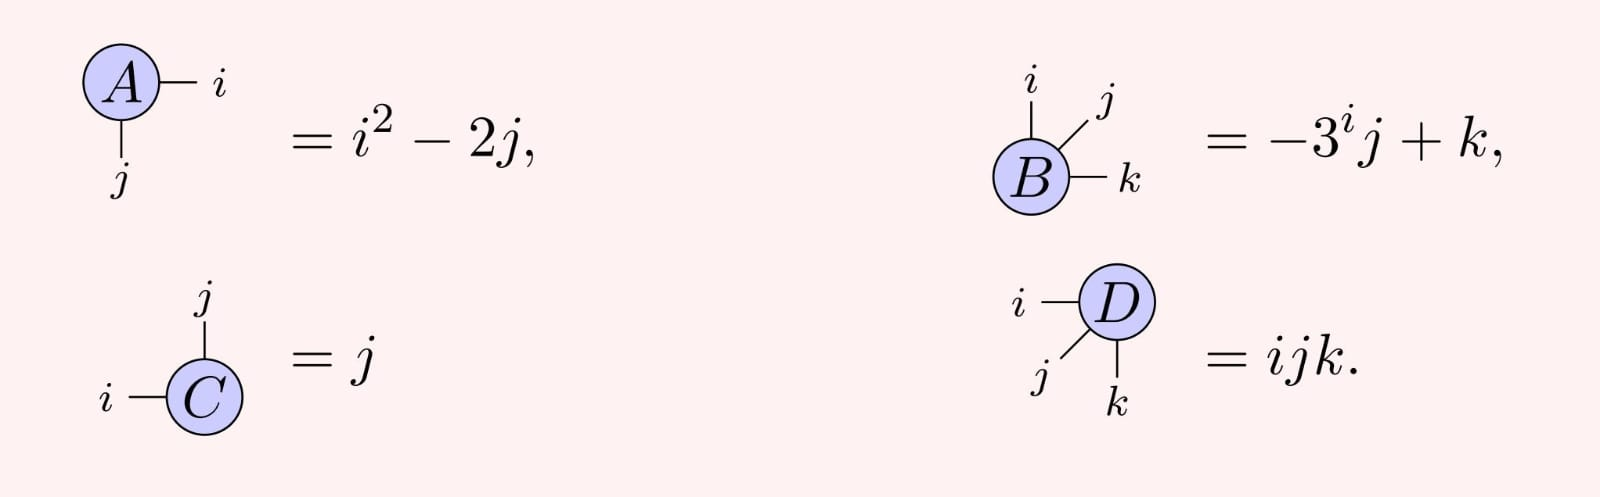
\includegraphics[width=0.6\linewidth]{images/tensorq1-1.jpeg}%
    \caption{Definitions of $A$, $B$, $C$ and $D$, Eqs.\eqref{def}}%
\end{figure}%

Calculate the value of the tensor network of Eq.~(1.22).

\begin{figure}[H]\centering
    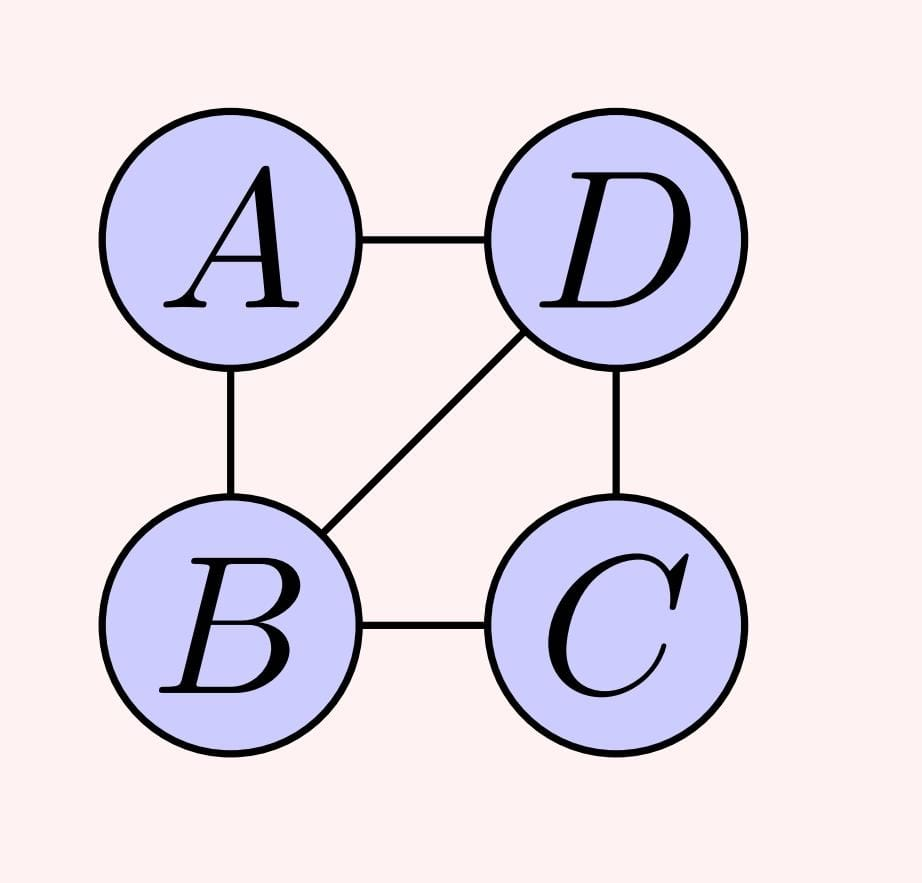
\includegraphics[width=0.25\linewidth]{images/tensorq1-2.jpeg}%
    \caption{The network to be contracted, Eq.~(1.22).}%
\end{figure}
\end{problem}


% ============================================================== solutions ===

\begin{solution}
There is no free index, so this is a scalar (the number of lines equal the number of indexed summed and must be consistent with the ordering $A_{i,j}, B_{i,j,k}$ to differentiate weach element of the tensor)
\begin{equation}
\begin{split}
     T &= \sum_{a,b,c,d,e} A_{a,b}B_{b,c,d}C_{d,e}D_{a,c,e}\\
     &= \sum_{a,b,c,d,e=0}^{2} (a^2  -2b)(-3^bc+d)(e)(ace)\\
     &= 1080
\end{split}
\end{equation}


\end{solution}


\attempt{
  date        = 2026-09-14,
  time        = 5min,
  difficulty  = 1,
  how it went = ,
}

\end{entry}
\begin{entry}{Q012}{Bubbling a network into a contraction table}

\entrymeta{
  topic   = {Tensor networks; contraction sequences; bubbling.},
  est     = $\sim$10 minutes,
  origin  = {Sourced. The original exercise; the worked example is reproduced so the
    required table format is unambiguous.},
  source  = {J.~C. Bridgeman and C.~T. Chubb, \emph{Hand-waving and Interpretive Dance:
    An Introductory Course on Tensor Networks}, J.~Phys.~A \textbf{50}, 223001 (2017),
    \href{https://arxiv.org/abs/1603.03039}{arXiv:1603.03039}, Section~1.6,
    Problem~2.},
  prereq  = {Section 1.4 (bubbling).},
  status  = open,
}

\begin{problem}
When a contraction is actually coded up, one contracts the tensors in one at a time and
must track, at each step, the open indices of the object built so far, the tensor being
absorbed, which indices are summed over in that step, and which new open indices the
incoming tensor contributes.

\begin{figure}[H]\centering
    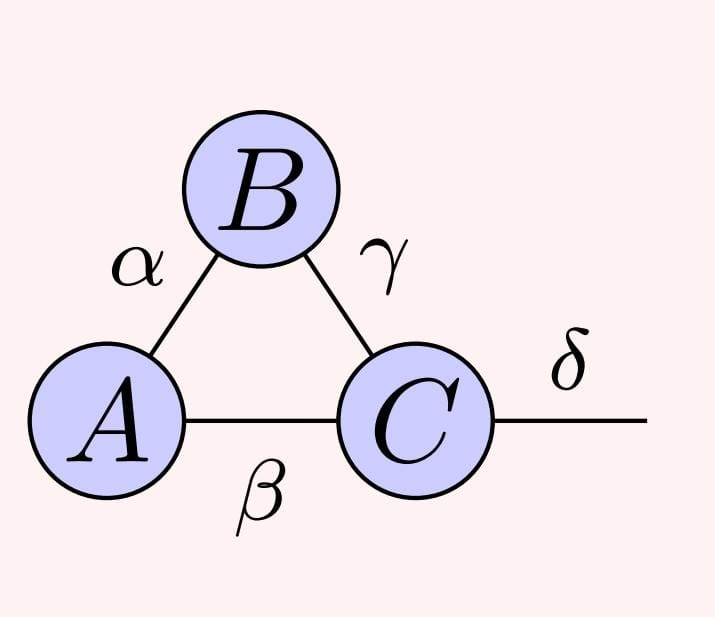
\includegraphics[width=0.2\linewidth]{images/tensorq2-1.jpeg}%
    \caption{The network of Eq.~(1.23), to be bubbled in alphabetical order.}%
\end{figure}


As an example, take the network of Eq.~(1.23): three tensors $A,B,C$ with bonds
$\alpha$ joining $A$ and $B$, $\beta$ joining $A$ and $C$, $\gamma$ joining $B$ and $C$,
and a free leg $\delta$ on $C$. Bubbling in alphabetical order gives


\begin{center}
\begin{tabular}{|c|c|c|c|}
\hline
Current & Tensor & Contract & New \\
\hline
--             & $A$ & --             & $\alpha,\beta$ \\
$\alpha,\beta$ & $B$ & $\alpha$       & $\gamma$ \\
$\beta,\gamma$ & $C$ & $\beta,\gamma$ & $\delta$ \\
\hline
\end{tabular}
\end{center}

Construct the corresponding table for the network of Eq.~(1.24), again bubbling in
alphabetical order.

\begin{figure}[H]\centering
    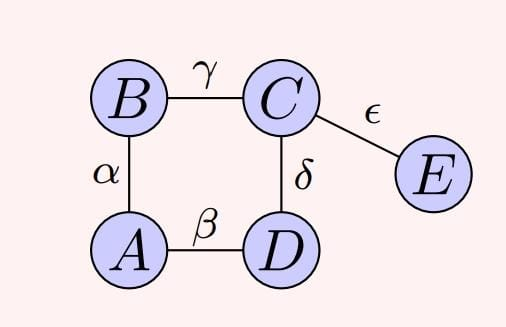
\includegraphics[width=0.2\linewidth]{images/tensorq2-2.jpeg}%
    \caption{The network of Eq.~(1.24), to be bubbled in alphabetical order}%
\end{figure}

and state the largest rank reached by the intermediate object, and whether a different
bubbling order would reduce it.

\end{problem}

% ============================================================== solutions ===

\begin{solution}
.
\vspace{0.1cm}
\begin{center}
\begin{tabular}{|c|c|c|c|}
\hline
Current & Tensor & Contract & New \\
\hline
--                      & $A$ & --          & $\alpha,\beta$ \\
  $\alpha,\beta$        & $B$ & $\alpha$    & $\gamma$   \\
 $\beta,\gamma$         & $C$ &  $\gamma$   &  $\delta,\epsilon$ \\
$\beta,\delta,\epsilon$ & $D$ &   $\delta,\beta$  & -- \\
            $\epsilon$  & $E$ &   $\epsilon$      &  -- \\
\hline
\end{tabular}
\end{center}
\vspace{0.1cm}
The largest rank is achieved after adding the tensor $C$ ($-A-B-C=$), where in this intermediate step we have a $\rank=3$ tensor. We could reduce the highest intermediate rank by starting from $E$, then going to $C$, we would contract $\epsilon$ and the intermediate tensor would be $\rank=2$, then, we can follow the adjacent $\rank=2$ tensors in the orders $B,A,D$ or $D,A,B$, on both cases at least one index is contracted and at most one is added, keeping the $\rank$ always lower or equal to $2$.
\end{solution}



\attempt{
  date        = 2026-09-14,
  time        = 10min,
  difficulty  = 1,
  how it went = ,
}

\end{entry}

\daysession{9}{2026-09-15}
\begin{entry}{Q013}{Counting colourings with tensor networks}

\entrymeta{
  topic   = {Tensor networks; graph colouring; counting complexity.},
  est     = $\sim$30 minutes total --- longer than the usual daily entry.
    Part (a) alone is $\sim$12 minutes and is the core; (b) and (c) may be done
    in a second sitting.,
  origin  = {Sourced. The original exercise; the definitions of $e$ and $n$ from
    Section~1.5 are inlined so the statement stands alone.},
  source  = {J.~C. Bridgeman and C.~T. Chubb, \emph{Hand-waving and Interpretive Dance:
    An Introductory Course on Tensor Networks}, J.~Phys.~A \textbf{50}, 223001 (2017),
    \href{https://arxiv.org/abs/1603.03039}{arXiv:1603.03039}, Section~1.6,
    Problem~3.},
  prereq  = {Section 1.5 (computational complexity).},
  status  = open,
}

\begin{problem}
Recall the two binary tensors of Section~1.5. The tensor $e$ takes the value $1$ if and
only if all of its indices are equal, and $0$ otherwise; the tensor $n$ takes the value
$1$ if and only if all of its indices differ, and $0$ otherwise. Given an arbitrary
graph, build a tensor network by placing an $e$ tensor at each vertex and an $n$ tensor
in the middle of each edge, inheriting the connectivity of the graph, as in
Eq.~(1.19).

\begin{figure}[H]\centering
    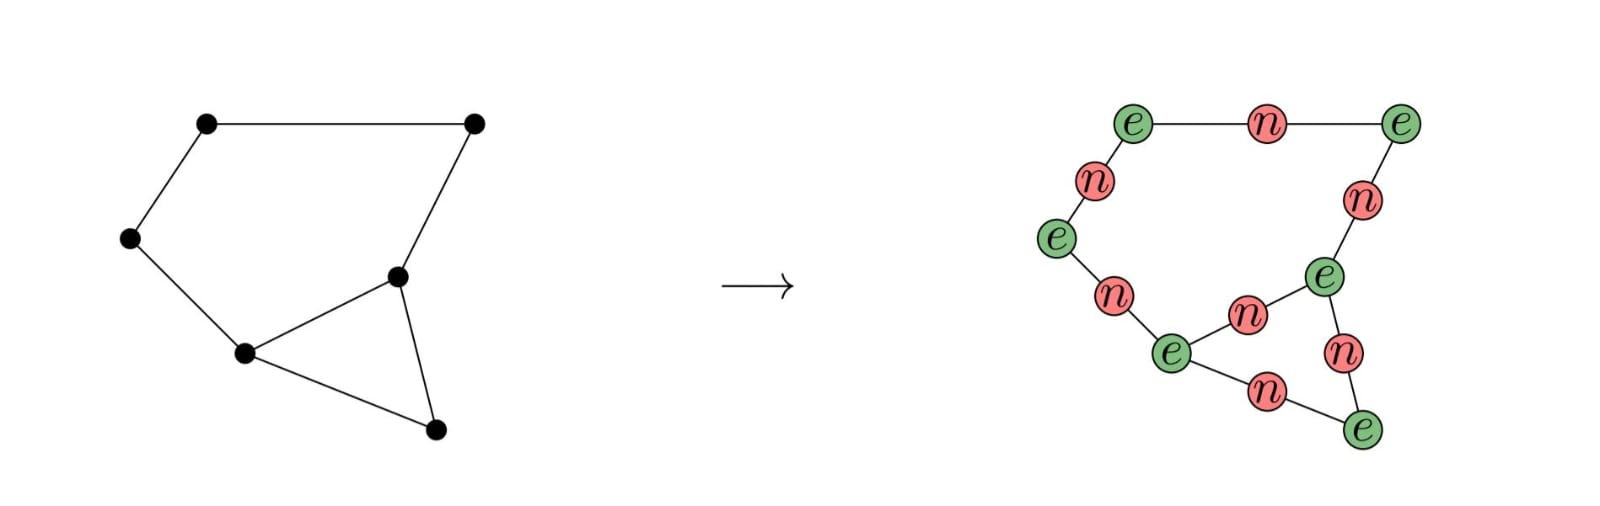
\includegraphics[width=0.7\linewidth]{images/tensorq3-1.jpeg}%
    \caption{The graph of Eq.~(1.19) and the tensor network built from it.}%
\end{figure}%

With $q$-dimensional indices, the nonzero contributions to this network are exactly the
vertex $q$-colourings of the graph, so its contraction counts them.

\begin{enumerate}[label=\textbf{(\alph*)},leftmargin=*]
  \item Calculate the contraction of the network of Eq.~(1.19) for bond dimension $q$,
        i.e.\ the number of three-colourings of the corresponding graph.
  \item Using the $e$ and $n$ tensors, construct a tensor network whose contraction gives
        the number of \emph{edge} colourings. For a planar graph, construct an analogous
        network counting \emph{face} colourings.
\end{enumerate}


\end{problem}

% ============================================================== solutions ===

\begin{solution}[Part (a)]
The equivalent tensor of e connected to two n, is
\begin{equation}
\begin{split}
    x_{a,b} &= \sum_{i,j}n_{a,i}e_{i,j}n_{j,b}\\
    &= \sum_{i,j} (1-\delta_{a,i})\delta_{i,j}(1-\delta_{j,b})\\
    &= \sum_{i} (1-\delta_{a,i})(1-\delta_{i,b})\\
    &= \delta_{a,b} + (q-2)
\end{split} 
\end{equation}

% requires \usepackage{tikz}
\usetikzlibrary{fit}
% requires \usetikzlibrary{fit}
\begin{figure}[H]\centering
\resizebox{\linewidth}{!}{%
\begin{tikzpicture}[
  every node/.style={font=\footnotesize},
  ten/.style={circle,draw,minimum size=5.5mm,inner sep=0pt},
  blu/.style={ten,fill=blue!20},
  red/.style={ten,fill=red!35},
  yel/.style={ten,fill=yellow!55},
  grn/.style={ten,fill=green!35},
  cut/.style={draw,dashed,thick,rounded corners,inner sep=3pt},
]

%=================== PANEL 1 : original, relaid out ===================
\begin{scope}[shift={(0,0)}]
  % upper branch: v5 - v3 - v1 - v2 - v4
  \node[blu] (v1) at (2.0, 2.6) {$e$};
  \node[blu] (nb) at (1.2, 2.3) {$n$};
  \node[blu] (v3) at (0.4, 2.0) {$e$};
  \node[blu] (nc) at (0.2, 1.0) {$n$};
  \node[blu] (na) at (2.8, 2.3) {$n$};
  \node[blu] (v2) at (3.6, 2.0) {$e$};
  \node[blu] (nd) at (3.8, 1.0) {$n$};
  % axis
  \node[blu] (v5) at (0.0, 0.0) {$e$};
  \node[blu] (nn) at (2.0, 0.0) {$n$};
  \node[blu] (v4) at (4.0, 0.0) {$e$};
  % lower branch: v5 - v6 - v4
  \node[blu] (nf) at (1.2,-1.5) {$n$};
  \node[blu] (v6) at (2.0,-1.9) {$e$};
  \node[blu] (ng) at (2.8,-1.5) {$n$};

  \draw (v5)--(nc)--(v3)--(nb)--(v1)--(na)--(v2)--(nd)--(v4);
  \draw (v5)--(nn)--(v4);
  \draw (v5) to[bend right=12] (nf);
  \draw (nf)--(v6)--(ng);
  \draw (ng) to[bend right=12] (v4);

  \node[cut,red!80!black,fit=(nc)(v3)(nb)] {};
  \node[cut,red!80!black,fit=(na)(v2)(nd)] {};
  \node[cut,red!80!black,fit=(nf)(v6)(ng)] {};
\end{scope}

\node at (5.1,0.3) {\Large$\to$};

%=================== PANEL 2 : after x-reduction ===================
\begin{scope}[shift={(6.0,0)}]
  \node[blu] (w1) at (2.0, 2.3) {$e$};
  \node[red] (x2) at (0.7, 1.5) {$x$};
  \node[red] (x1) at (3.3, 1.5) {$x$};
  \node[blu] (w5) at (0.0, 0.0) {$e$};
  \node[blu] (nn) at (2.0, 0.0) {$n$};
  \node[blu] (w4) at (4.0, 0.0) {$e$};
  \node[red] (x3) at (2.0,-1.5) {$x$};

  \draw (w5)--(x2)--(w1)--(x1)--(w4);
  \draw (w5)--(nn)--(w4);
  \draw (w5) to[bend right=15] (x3);
  \draw (x3) to[bend right=15] (w4);

  \node[cut,yellow!60!black,fit=(x2)(w1)(x1)] {};
  \node[cut,green!50!black,fit=(w5)(nn)(x3)(w4)] {};
\end{scope}

\node at (11.1,0.3) {\Large$\to$};

%=================== PANEL 3 : y over z ===================
\begin{scope}[shift={(11.9,0)}]
  \node[yel] (y) at (0.9, 1.3) {$y$};
  \node[grn] (z) at (0.9,-0.6) {$z$};
  \draw (y) to[bend left=38]  (z);
  \draw (y) to[bend right=38] (z);
  \node[cut,gray,fit=(y)(z)] {};
\end{scope}

\node at (13.9,0.3) {\Large$\to$};

%=================== PANEL 4 : scalar ===================
\begin{scope}[shift={(14.5,0)}]
  \node[ten,fill=gray!40] at (0.5,0.3) {};
\end{scope}

\end{tikzpicture}}
\caption{Contraction of the network of Eq.~(1.19), redrawn so that the three
$n$--$e$--$n$ chains occupy disjoint regions. Red contours mark the chains replaced by
$x$; the yellow contour is $x$--$e$--$x\to y$; the green contour is the pair of vertices
joined by the parallel $n$ and $x$ bonds, $\to z$. Contracting $y$ against $z$ across the
double bond leaves a scalar.}
\end{figure}%

The upper part inside the yellow dashed line is equivalent to 
\begin{equation}
\begin{split}
    y_{a,b}&= \sum_{i,j}x_{a,i}e_{i,j}x_{j,b}\\
    &=\sum_{i,j} x_{a,i}\delta_{i,j}x_{j,b}\\
    &= \sum_{i} x_{a,i}x_{i,b}\\
    &= \sum_i (q-2)^2 + (q-2)(\delta_{a,i}+\delta_{i,b}) + \delta_{a,i}\delta_{i,b}\\
    &= q(q-2)^2+ 2(q-2) + \delta_{a,b}
\end{split}
\end{equation}
whereas for the below part inside the green dashed line is equivalent to 

\begin{equation}
\begin{split}
    z_{a,b}&= \sum_{i,j,k,l}e_{a,i,j}x_{j,l}n_{i,k}e_{k,l,b}\\
    &=\sum_{i,j,k,l}\delta_{a,i,j}x_{j,l}n_{i,k}\delta_{k,l,b}\\
    &= x_{a,b}n_{a,b}
\end{split}
\end{equation}
so
\begin{equation}
\begin{split}
    T&=\sum_{a,b} z_{a,b}y_{a,b}\\
    &= \sum_{a,b} (q(q-2)^2+ 2(q-2) + \delta_{a,b})((q-2)+\delta_{a,b})(1-\delta_{a,b})\\
    &= q(q-1)(q-2)^2[q^2-2q+2]
\end{split}
\end{equation}


\end{solution}

\begin{solution}[Part (b)]
These tensor $e$ and $n$ allows one to generalize the q-colouring counting problem by simple using $e$ in place of the counting object and $n$ used as the "adjacency mediator"  forcing that no adjacent objects have the same colour. To count the number of edges colouring you may draw a tensor network with $e$ in the edges and $n$ in the vertices, meanwhile to count the number of face colouring you draw a network with $e$ in the face( inside each polygon) and $n$ in the commom edges of the polygons. 
\end{solution}





\attempt{
  date        = ,
  time        = ,
  difficulty  = ,
  how it went = ,
}

\end{entry}

\daysession{10}{2026-09-17}
\begin{entry}{Q014}{Grassmann integrals and the trace of a Floquet operator}

\entrymeta{
  topic   = {Grassmann (Berezin) integration; Gaussian fermionic integrals;
    field-theory approach to quantum chaos.},
  est     = $\sim$25 minutes --- longer than the usual daily entry; part (c) is the core
    and may be done separately.,
  origin  = {Adapted. Reconstructed from a lecture exercise; the Grassmann axioms are
    inlined and the time-lattice conventions fixed so the statement is self-contained.},
  source  = {T. Micklitz, lectures on \emph{Field-Theory Approach to Quantum Chaos},
    School on Analytical and Numerical Methods for Disordered Quantum Systems.},
  prereq  = {None beyond linear algebra; all Grassmann conventions are stated below.},
  status  = open,
}

\begin{problem}
\textbf{Conventions.} Let $\psi_1,\dots,\psi_n,\bar\psi_1,\dots,\bar\psi_n$ be
\emph{Grassmann variables}: generators of an associative algebra over $\CC$ subject to
\[
  \{\psi_i,\psi_j\}=\{\bar\psi_i,\bar\psi_j\}=\{\psi_i,\bar\psi_j\}=0
  \qquad\text{for all } i,j,
\]
so in particular $\psi_i^{2}=\bar\psi_i^{2}=0$. Every function of them is a polynomial
of degree at most one in each generator. \emph{Berezin integration} in a single variable
is the linear map defined by
\begin{equation}
    \int d\psi\;1=0,
  \qquad
  \int d\psi\;\psi=1,
  \label{grassman identity}
\end{equation}

and the differentials $d\psi_i,d\bar\psi_i$ anticommute with each other and with all
generators. For $n$ pairs write
\[
  D(\bar\psi,\psi):=\prod_{i=1}^{n} d\bar\psi_i\, d\psi_i ,
  \qquad\text{normalised so that}\qquad
  \int D(\bar\psi,\psi)\;\prod_{i=1}^{n}\psi_i\bar\psi_i \;=\;1 .
\]
For $A\in\CC^{n\times n}$ set $\bar\psi A\psi:=\sum_{i,j}\bar\psi_i A_{ij}\psi_j$.

\begin{enumerate}[label=\textbf{(\alph*)},leftmargin=*]
  \item Prove that
        \[
          \int D(\bar\psi,\psi)\; e^{-\bar\psi A\psi} \;=\;\det A .
        \]
  \item Prove that, for $A$ invertible,
        \[
          \int D(\bar\psi,\psi)\; e^{-\bar\psi A\psi}\,\psi_a\bar\psi_b
          \;=\;\det A\;\bigl(A^{-1}\bigr)_{ab} .
        \]
  \item Let $U_0$ be a unitary on $\CC^{N}$ (one step of a Floquet evolution), and let
        the discrete time lattice be $\{0,1,\dots,t\}$, on which the lowering operator
        $T_-$ acts by $T_-\ket{\tau}=\ket{\tau-1}$, i.e.
        $(T_-)_{\tau,\tau'}=\delta_{\tau,\tau'-1}$. Take Grassmann variables
        $\psi_{(i,\tau)},\bar\psi_{(i,\tau)}$ indexed by $i\in\{1,\dots,N\}$ and
        $\tau\in\{0,\dots,t\}$, and set
        \[
          A=\id-U_0\otimes T_- .
        \]
        Show that $\det A=1$, compute $\bigl(A^{-1}\bigr)_{(i,\tau),(j,\tau')}$, and
        conclude that
        \[
          \int D(\bar\psi,\psi)\; e^{-\bar\psi A\psi}
          \sum_{a=1}^{N}\psi_{(a,0)}\,\bar\psi_{(a,t)}
          \;=\;\Tr\bigl(U_0^{\,t}\bigr).
        \]
        Explain why an insertion diagonal in the time index, $\sum_a
        \psi_{(a,\tau)}\bar\psi_{(a,\tau)}$, cannot produce this result.
\end{enumerate}
\end{problem}

% ============================================================== solutions ===

\begin{solution}[Part (a)]
Since $\psi_i^{2}=\bar\psi_i^{2}=0$, we have that 
\begin{equation}
    e^{-\bar\psi A\psi}= \prod_{i,j}(1 -  \bar\psi_i A_{ij}\psi_j)=O(0)+O(2)+...+O(2n)
\end{equation}
where here $O(2k)$ represent the term where there is a product of $2k$ Grassmann variables, i.e.,
\begin{equation*}
\begin{split}
    O(2k)= (-1)^k\sum_{\substack{i_1\neq...\neq i_k\\j_1\neq...\neq j_k}} \prod_{x=1}^{k}\bar\psi_{i_x}A_{i_x,j_x}\psi_{j_x}
\end{split}
\end{equation*}
(notice that equal index leads to 0 contribution, $\psi_i^{2}=\bar\psi_i^{2}=0$ forcing the summation to be over different index) but from \eqref{grassman identity}, any term that doesn't have the full $2n$ Grassmann variables vanishes when integrated, $\int D(\bar\psi,\psi) O(2k)=0,\ k<n$, then 
\begin{equation}
\begin{split}
    \int D(\bar\psi,\psi)\; e^{-\bar\psi A\psi} = \int D(\bar\psi,\psi) \sum_{\substack{i_1\neq...\neq i_n\\j_1\neq...\neq j_n}} \prod_{x=1}^{n}\bar\psi_{i_x}A_{i_x,j_x}\psi_{j_x}
\end{split}
\end{equation}
which can be rewritten in the permutation notation 
\begin{equation}
\begin{split}
    \int D(\bar\psi,\psi)\; e^{-\bar\psi A\psi} =& (-1)^n\int D(\bar\psi,\psi) \sum_{\sigma \in S_n} \prod_i^n \bar\psi_i A_{i\sigma(i)}\psi_{\sigma(i)}\\
    =& (-1)^n\sum_{\sigma \in S_n}\int D(\bar\psi,\psi)\prod_i\bar\psi_i \psi_{\sigma(i)}A_{i \sigma(i)}.
\end{split}
\end{equation}
Now, due to the anti-commutativity of the Grassmann variables, we can rewrite the normalization condition and then derive for a generic permutation
\begin{equation}
   \int D(\bar\psi,\psi)\prod_i\bar\psi_i \psi_{i} =(-1)^n\implies\int D(\bar\psi,\psi)\prod_i\bar\psi_i \psi_{\sigma(i)}=(-1)^n\text{sign}(\sigma)
\end{equation}, where an even permutation would require an even number of exchanges to order the integral as products $\int d \psi \psi$, meanwhile an odd permutation requires an odd number of exchanges, leading to a $-$ sign overall, hence
\begin{equation}
\begin{split}
    \int D(\bar\psi,\psi)\; e^{-\bar\psi A\psi}
    =&\sum_{\sigma \in S_n}\text{sign}(\sigma)\prod_iA_{i \sigma(i)}\\
    =& \det (A
)\end{split}
\end{equation}
\end{solution}

\begin{solution}[Part (b)]
We can see the matrix itself as a list of complex variables, consider Einstein summation notation for an Euclidean norm, such that the expression can be written as (for the sake of precision consider $X_{i,j}$ the list of complex variables)
\begin{equation}
\begin{split}
    \int D(\bar\psi,\psi)\; e^{-\bar\psi A\psi}\psi_a \bar\psi_b
    =&\int D(\bar\psi,\psi)\; e^{-\bar\psi^\nu A_{\nu\mu}\psi^\mu}\psi_a \bar\psi_b\\
    =& \int D(\bar\psi,\psi)\; e^{-\bar\psi^\nu A_{\nu\mu}\psi^\mu}(-\bar\psi_b \psi_a) \\
    =&\bigg(\frac{\partial}{\partial X_{ba}}\int D(\bar\psi,\psi)\; e^{-\bar\psi^\nu X_{\nu\mu}\psi^\mu}\bigg)_{X=A}\\
    =& \bigg(\frac{\partial}{\partial X_{ba}}\det(X)\bigg)_{X=A}
\end{split}
\end{equation}
From Cramer's rule for the determinant, for any row $i$
\begin{equation*}
    \det X = \sum_{j}X_{ij}C_{ij}
\end{equation*}
where $C_{ij}$ is the cofactor in the corresponding position $i,j$, which depends on all variables of $X$ besides the ones that have either row $i$ or column $j$ (you eliminate the row $i$ and columns $j$ to calculate the determinant of the remaining matrix, to attain $C_{i,j}$), so taking the row $i=b$, we can write $\det X = \sum_{j}X_{bj}C_{bj}$. No element of the summation depends on $X_{ba}$ besides when $j=a$, so
\begin{equation*}
    \frac{\partial}{\partial X_{ba}}\det X = C_{ba}
\end{equation*}
Now, from Laplace's formula for the inverse, or cofactor method, the inverse is calculated precisely from the cofactor by
$$(X^{-1})_{ij} =\frac{C_{ji} }{\det X}$$
therefore
\begin{equation}
    \int D(\bar\psi,\psi)\; e^{-\bar\psi A\psi}\psi_a \bar\psi_b
    = \det A (A^{-1})_{ab}
\end{equation}
\end{solution}

\begin{solution}[Part (c)]
Defining properly the notation for the spatial and temporal degrees of freedom
\begin{equation}
\begin{split}
    \sum_{a,a',\tau,\tau'} \bar \psi_{(a,\tau)} (U^k_0\otimes T_-^k)_{(a,a'),(\tau,\tau')} \psi_{(a',\tau')}= \sum_{a,a',\tau,\tau'} \bar \psi_{(a,\tau)} (U^k_0)_{(a,a')}\otimes (T_-^k)_{(\tau,\tau')} \psi_{(a',\tau')}
\end{split}
\end{equation}
Now notice 
\begin{equation}
    T_-=\sum_{\tau=1}^{t}\ket{\tau-1}\bra{\tau}
=\begin{pmatrix}
0 & 1 & 0 & \cdots & 0 \\
0 & 0 & 1 & \ddots & \vdots \\
\vdots & \vdots & \ddots & \ddots & 0 \\
0 & 0 & \cdots & 0 & 1 \\
0 & 0 & \cdots & 0 & 0 \qquad 
\end{pmatrix},
\qquad
(T_-)_{\tau\tau'}=\delta_{\tau,\tau'-1}. \qquad \text{odering}\ \ket{0} = \begin{pmatrix}
    1\\
    ...\\
    0
\end{pmatrix}
\end{equation}
exponentiation of $T_-$ lower its own entries, leading to
\begin{equation}
T_-^{\,k}=\sum_{\tau=1}^{t}\ket{\tau-1}\bra{\tau}
=\begin{pmatrix}
0_{(t+1-k)\times k} & \id_{t+1-k} \\[2pt]
0_{k\times k} & 0_{k\times(t+1-k)}
\end{pmatrix},
\quad (T_-^{\,k})_{\tau\tau'}=\delta_{\tau,\tau'-k},,
\qquad T_-^{\,t+1}=0 ,
\end{equation}
Moreover, we have that $(T_-^k)_{0t} = \delta_{kt}$, which means that the we got apply the $T_-$ $t$ times in order to have an element in the last columns of the first row, meanwhile the condition $T_{-}^{t+1}=0$, makes $U_0\otimes T_-$ nilpotent, such that the inverse of $A=\id-U_0\otimes T_-$ can be calculated from the geometric series, 
\begin{equation}
    (\id -U_0\otimes T_-)^{-1}= \sum_{k=0}^t U_0^k \otimes T_{-}^k
\end{equation}
 thus
\begin{equation}
    (A^{-1})_{(a,0),(b,t)}= (U_0^t)_{a,b}
\end{equation}
Finally,
\begin{equation}
    A=\id-U_0\otimes T_-=
\begin{pmatrix}
\id_N & -U_0 & & & \\
 & \id_N & -U_0 & & \\
 & & \ddots & \ddots & \\
 & & & \id_N & -U_0 \\
 & & & & \id_N
\end{pmatrix}
\end{equation} such that $\det A=1$, therefore, using item b) 
\begin{equation}
    \int D(\bar\psi,\psi)\; e^{-\bar\psi A\psi}
          \sum_{a=1}^{N}\psi_{(a,0)}\,\bar\psi_{(a,t)}
          \;=\; \sum_a =\Tr\bigl(U_0^{\,t}\bigr).
\end{equation}
 



\end{solution}



\attempt{
  date        = 2026-09-15,
  time        = ,
  difficulty  = ,
  how it went = ,
}

\end{entry}
\begin{entry}{Q015}{From free to damped: the arc propagator at finite $\gamma$}

\entrymeta{
  topic   = {Discrete-time field theory; contour times; finite-difference Green
    functions; quantum chaos.},
  est     = $\sim$15 minutes,
  origin  = {Adapted. Reconstructed from a lecture exercise; the index conventions,
    the Heaviside convention and the structural part (a) are inlined so the statement
    stands alone.},
  source  = {T. Micklitz, lectures on \emph{Field-Theory Approach to Quantum Chaos},
    School on Analytical and Numerical Methods for Disordered Quantum Systems.
    Companion to \qref{Q016}.},
  prereq  = {None beyond finite differences.},
  status  = open,
}

\begin{problem}
\textbf{What this describes.} In the field theory of the previous entry, the object of
interest is not a single amplitude but a \emph{pair} of them: one propagating forward in
time and one backward, whose phases cancel and which therefore survive an average over
the random dynamics. The propagator $\Pi$ follows such a pair, and each of its legs
carries two times, one on each branch. The free theory has no scale: once formed, a pair
stays correlated forever. The interacting theory has one, $\gamma$, at which the two
branches lose their correlation; the exercise is to see that scale appear, and to see
what it means.

\textbf{Conventions.} Time is discrete, $n\in\ZZ$. Each leg carries a pair of contour
times $(n^{+},n^{-})$, forward and backward. Write the pair as a single label,
\[
  \mathbf n:=(n^{+},n^{-}),
  \qquad
  \Delta n:=n^{+}-n^{-}\ \ \text{(relative time)},
  \qquad
  \bar n:=\tfrac12\bigl(n^{+}+n^{-}\bigr)\ \ \text{(mean time)} ,
\]
so that $\mathbf n\mapsto(\Delta n,\bar n)$ is a change of coordinates on the set of
pairs: $\Delta n$ records how far apart on the two branches the pair sits, and $\bar n$
how far along both have travelled together.

The propagator $\Pi_{\mathbf n_2,\mathbf n_1}$ is a kernel from the incoming pair
$\mathbf n_1$ to the outgoing pair $\mathbf n_2$. Kernels compose by summation over the
repeated pair,
\[
  (KL)_{\mathbf n_2,\mathbf n_1}
  :=\sum_{\mathbf m}K_{\mathbf n_2,\mathbf m}\,L_{\mathbf m,\mathbf n_1},
  \qquad
  \bigl(\id\bigr)_{\mathbf n_2,\mathbf n_1}
  =\delta_{n_2^{+},n_1^{+}}\,\delta_{n_2^{-},n_1^{-}} ,
\]
and act on the outgoing label only. Let $T$ be the kernel that advances \emph{both}
contour times by one unit --- one step of the dynamics, applied to both branches at
once,
\[
  T_{\mathbf n,\mathbf m}
  :=\delta_{n^{+},\,m^{+}+1}\;\delta_{n^{-},\,m^{-}+1},
\]
and set $d:=\id-T$, the discrete counterpart of a time derivative. Write $\Theta(u)=1$
for $u\ge0$ and $\Theta(u)=0$ for $u<0$, so that $\Pi$ is supported on outgoing times
later than incoming ones. Finally let $D_0>0$ be the normalisation constant of the notes
and $\gamma>0$ a damping rate.

\begin{enumerate}[label=\textbf{(\alph*)},leftmargin=*]
  \item Show that $T$ preserves the relative time and lowers the mean time by one:
        in the coordinates $(\Delta n,\bar n)$,
        \[
          T_{\mathbf n,\mathbf m}
          =\delta_{\Delta n,\Delta m}\;\delta_{\bar n,\,\bar m-1}.
        \]
        Deduce that if $K_{\mathbf n_2,\mathbf n_1}
        =\delta_{\Delta n_2,\Delta n_1}\,f(\bar n_2-\bar n_1)$ for some
        $f:\ZZ\to\CC$, then
        \[
          (dK)_{\mathbf n_2,\mathbf n_1}
          =\delta_{\Delta n_2,\Delta n_1}\bigl[f(u)-f(u-1)\bigr],
          \qquad u:=\bar n_2-\bar n_1 ,
        \]
        so that the problem reduces to a one-dimensional recursion in $u$.

  \item \emph{Free theory.} Verify that the propagator for the free theory
        \[
          \Pi_{\mathbf n_2,\mathbf n_1}
          =\frac{1}{D_0}\,\delta_{\Delta n_2,\Delta n_1}\,\Theta(\bar n_2-\bar n_1)
        \]
        satisfies
        \[
          (d\,\Pi)_{\mathbf n_2,\mathbf n_1}
          =\frac{1}{D_0}\,\delta_{\Delta n_2,\Delta n_1}\,
            \delta_{\bar n_2,\bar n_1} .
        \]

  \item \emph{Interacting theory.} The propagator for the interacting theory (with mass) is
        \[
          \Pi^{\mathrm{arc}}_{\mathbf n_2,\mathbf n_1}
          =\frac{1}{D_0}\,\delta_{\Delta n_2,\Delta n_1}\,
            \frac{\Theta(\bar n_2-\bar n_1)}{(1+\gamma)^{\,\bar n_2-\bar n_1+1}} .
        \]
        Show that 
        \[
          \bigl[(d+\gamma)\,\Pi^{\mathrm{arc}}\bigr]_{\mathbf n_2,\mathbf n_1}
          =\frac{1}{D_0}\,\delta_{\Delta n_2,\Delta n_1}\,
            \delta_{\bar n_2,\bar n_1} ,
        \]
        i.e.\ $\Pi^{\mathrm{arc}}$ is the Green function of $d+\gamma$ with the same
        right-hand side as in the free case. Note where the factor
        $(1+\gamma)^{-u}$ disappears from the final answer.

   \item \emph{The lattice scale.} Fix the relative time and compare successive mean
        times: show that for $\bar n_2\ge\bar n_1$ the ratio
        \[
          \frac{\Pi^{\mathrm{arc}}_{\,(\Delta n,\,\bar n_2+1),\,\mathbf n_1}}
               {\Pi^{\mathrm{arc}}_{\,(\Delta n,\,\bar n_2),\,\mathbf n_1}}
        \]
        does not depend on $\bar n_2$, and identify it. The decay is therefore
        geometric: the same fraction of the amplitude is lost at every step, regardless
        of how long the pair has already survived.

        Explain why this is the expected structure rather than a coincidence, by reading
        it off the equation $\Pi^{\mathrm{arc}}=\bigl[(1+\gamma)\id-T\bigr]^{-1}$ that
        (c) establishes: each application of $T$ advances both branches by one step of
        the dynamics, and each such step is accompanied by the same factor. What
        property of the underlying dynamics does this memorylessness reflect, and what
        would have to change for the loss per step to depend on $\bar n_2-\bar n_1$?


  \item \emph{The approximation.} Show that $(1+\gamma)^{-u}=e^{-\gamma u}$ up to a
        relative error controlled by $\gamma^{2}u$, and say why it is this product,
        rather than $\gamma$ alone, that must be small for the exponential form to hold. Determine also the sign of
        the discrepancy: does the lattice decay faster or slower than the exponential?

  \item \emph{The continuum limit.} Take as given that the Green function of
        $\partial_{\mathcal T}+\Gamma$ is $\Theta(\mathcal T)\,e^{-\Gamma\mathcal T}$,
        where the constant $\Gamma$ added to a first-order derivative is a \emph{mass
        term} and fixes the only scale of the continuum theory, $\tau=1/\Gamma$. Let
        $\delta t$ be the physical duration of one lattice step, so that
        $\mathcal T=u\,\delta t$ and $\gamma=\Gamma\,\delta t$. Using~(e), show that
        $\Pi^{\mathrm{arc}}$ converges to the continuum Green function as
        $\delta t\to0$, and state precisely which quantity is held fixed in the limit
        and which is sent to zero. Explain why the limit cannot be taken at fixed $u$,
        nor at fixed $\gamma$, and why the physically meaningful statement is that
        $\delta t$ disappears from the answer while $\tau$ does not: the scale belongs
        to the theory, the lattice spacing to its description. How many lattice steps
        does one lifetime $\tau$ contain, and what does that number have to be for the
        continuum description to apply?
\end{enumerate}
\end{problem}

% ============================================================== solutions ===

\begin{solution}[a]
$n^+=m^+ - 1$ and $n^-=m^- - 1$ if and only if $n^+ - n^- = m^+ - m^-$ and $\frac{n^+ + n^-}{2} =\frac{m^+ + m^-}{2} -1$, thus
\[
          T_{\mathbf n,\mathbf m}
          =\delta_{\Delta n,\Delta m}\;\delta_{\bar n,\,\bar m+1}.
        \]
Applying $T$ to such $K$
\begin{equation}
    \begin{split}
        (TK)_{\mathbf n_2, \mathbf n_1} &= \sum_{\mathbf m} T_{\mathbf n_2,\mathbf{ m}}K_{\mathbf{ m}, \mathbf n_1}\\
        &= \sum_{\Delta m, \bar m} \delta_{\Delta n_2,\Delta m}\;\delta_{\bar n_2,\,\bar m+1} \delta_{\Delta m,\Delta n_1}\,f(\bar m - \bar n_1) \\
        &=  \delta_{\Delta n_2,\Delta n_1}f(\bar n_2 -1 -n_1)\\
        &=  \delta_{\Delta n_2,\Delta n_1}f(u-1)
    \end{split}
\end{equation}
Therefore, it follows directly when applying $d$

\end{solution}

\begin{solution}[b]
From a)
\begin{equation}
   (d\,\Pi)_{\mathbf n_2,\mathbf n_1}
          =\frac{1}{D_0}\,\delta_{\Delta n_2,\Delta n_1}\,
            \big(\Theta({\bar n_2-\bar n_1}) - \Theta({\bar n_2-\bar n_1}-1)\big)
\end{equation}
Now if $\bar n_2-\bar n_1-1 \geq 0$, both $\Theta$ are equal to 1, leading to a null for the finite difference. If $\bar n_2-\bar n_1<0$, both vanish. So the finite difference only survives when $\bar n_2-\bar n_1 = 0$. Therefore,
\[
          (d\,\Pi)_{\mathbf n_2,\mathbf n_1}
          =\frac{1}{D_0}\,\delta_{\Delta n_2,\Delta n_1}\,
            \delta_{\bar n_2,\bar n_1} .
        \]
\end{solution}

\begin{solution}[c]
Applying item a) we get that 
\begin{equation}
  d \Pi^{\mathrm{arc}}_{\mathbf n_2,\mathbf n_1}
          =\frac{1}{D_0}\,\delta_{\Delta n_2,\Delta n_1}\,
            \left(\frac{\Theta(\bar n_2-\bar n_1)}{(1+\gamma)^{\,\bar n_2-\bar n_1+1}}-\frac{\Theta(\bar n_2-\bar n_1-1)}{(1+\gamma)^{\,\bar n_2-\bar n_1}} \right) .
\end{equation}
Meanwhile 
\begin{equation}
\begin{split}
    \gamma \Pi^{\mathrm{arc}}_{\mathbf n_2,\mathbf n_1}
          &=\frac{1}{D_0}\,\delta_{\Delta n_2,\Delta n_1}\,
            \frac{\Theta(\bar n_2-\bar n_1)}{(1+\gamma)^{\,\bar n_2-\bar n_1}}\left(\frac{\gamma}{1+\gamma} \right) \\
         &=\frac{1}{D_0}\,\delta_{\Delta n_2,\Delta n_1}\,
            \frac{\Theta(\bar n_2-\bar n_1)}{(1+\gamma)^{\,\bar n_2-\bar n_1}}\left(1-\frac{1}{1+\gamma} \right)  
\end{split}
\end{equation}
 To conclude, we must notice that after summing both expressions, the delta makes the only non-zero contribution occur when $\bar n_2 = \bar n_1$, reducing the exponent of the denominator to 0
 \begin{equation}
 \begin{split}
      (d+\gamma) \Pi^{\mathrm{arc}}_{\mathbf n_2,\mathbf n_1}
          &=\frac{1}{D_0}\,\delta_{\Delta n_2,\Delta n_1}\,
            \frac{\delta_{\bar n_2,\bar n_1}}{(1+\gamma)^{\,\bar n_2-\bar n_1}} \\
            &= \frac{1}{D_0}\,\delta_{\Delta n_2,\Delta n_1}\,
            \delta_{\bar n_2,\bar n_1} 
 \end{split}
 \end{equation}
This can be seen as the mass term for the theory
\end{solution}

\begin{solution}[d]
The ratio is given by 
\begin{equation*}
        (1+\gamma)^{-1}
\end{equation*}
which is smaller than $1$, reflecting the expected damping.
Inverting the expression for item c) (the right-hand side can be seen as proportional to the identity) and applying the geometric series, which converges even we stop looking at finite time since $(1+\gamma)^{-1} <1$ for $\gamma>0$. 

\begin{equation}
\begin{split}
    \Pi^{\text{arc}}=&\frac{1}{D_0} \bigl[(1+\gamma)\id-T\bigr]^{-1}\\
    =& \frac{1}{D_0 (1+\gamma)} \bigl[\id- \frac{1}{(1+\gamma)}T\bigr]^{-1}\\
    =& \frac{1}{D_0 (1+\gamma)} \sum_{k=0}^\infty \left(\frac{1}{(1+\gamma)}T\right)^k
\end{split}
\end{equation}

such that $T^k$ is accompanied by a factor $\frac{1}{(1+\gamma)^k}$, i.e., each lattice evolution adds the damping.

The memorylessness is a reflection that the circuit applies the same random matrix at each time step. Therefore, the theory itself must reflect through a memoryless Lagrangian $d + \gamma$, where both the finite difference and the constant $\gamma$ are translational invariant objects. To change that, we would need a function of $\bar n_2 -\bar n_1$ instead of a constant to the theory. 

\end{solution}






\begin{solution}[e]
We can rewrite the binomial power as
\begin{equation}
    (1+\gamma)^{-u} = e^{-u\ln(1+\gamma)} = e^{-u \gamma } e^{u(\gamma -\ln (1+\gamma))}
\end{equation}
Analyzing the expansion for the logarithm, we see that, for $|\gamma|<1$,
\begin{equation*}
    \ln(1+\gamma)=\sum_{k=1}^{\infty} \frac{(-1)^{k+1}}{k} \gamma^k = \gamma - \sum_{k=2}^{\infty} \frac{(-1)^{k}}{k} \gamma^k 
\end{equation*}
for a more explicit visualization, notice that this implies
\begin{equation}
    \gamma - \ln(1+\gamma) = \frac{1}{2}\gamma^2 + O(\gamma^3) =  \frac{1}{2}\gamma^2 + \gamma^2O(\gamma).
    \label{order magnitude}
\end{equation}

The relative error is measured by the exponential $e^{u(\gamma -\ln (1+\gamma))}$, which is smaller when the exponent is close to 0. From eq\eqref{order magnitude} one can see this is the case when both $u\gamma^2$ are $\gamma$, themselves are small. The first condition enforces the overall factor being small, while the latter makes the sum it multiplies, $\frac{1}{2} + O(\gamma)$ something of order $\sim 1$, not counterbalancing the decrease of $u\gamma^2$. 
\begin{equation}
\begin{split}
    \frac{(1+\gamma)^{-u}-e^{-\gamma u }}{e^{-\gamma u }} &= e^{u(\gamma -\ln (1+\gamma))} -1 \\
    &= e^{u\gamma^2\left(\frac{1}{2}+O(\gamma)\right)} -1\\
    &= u\gamma^2\left(\frac{1}{2}+O(\gamma)\right) + \sum_{k=1}^{\infty} \frac{1}{k!} \left(u\gamma^2\left(\frac{1}{2}+O(\gamma)\right)\right)^k
\end{split} 
\end{equation}
Which for small enough $\gamma$, can be seen as 
\begin{equation}
    O(u\gamma^2)
\end{equation}
And the relative errors is positive so the exponential (as one should expect) decays faster.
\end{solution}

\begin{solution}[f]
    To go for the continuum limit, one needs that the lattice step duration $\delta t$ becomes infinitesimally small to reproduce the continuity. The previous item set the condition for mathematical convergence, nonetheless, the "limiting theory" only reproduces the same continuum theory if their scales are same, i.e., we set $\tau = \delta t/\gamma$ constant through the limit. 

    The time it takes to complete $u$ lattice steps is $\mathcal T=u\delta t$, whereas the lifetime is $\tau = \delta t/\gamma$, so one lifetime requires $u= 1/\gamma$ time steps, which, as expected, should go to infinity in the continuum limit. $\delta t$ can be seen as a unit of measure, like meters or seconds, connecting the model to actual physical implementation. 
    All quantities are dimensionless in the lattice theory. Thus, $\delta t$ is necessary to actually analyze the time the pairs take to survive, yet it does not dictate how quantities relate on a physical theory.
    
    To compare the theory with the continuum theory at time $\mathcal T$ (view it as point-wise approximation, though by the bound in (e), the convergence is in fact uniform on bounded intervals of $\mathcal{T}$), we approximate it by $u \delta t$, whereas the time scale itself must be held constant $\tau = \delta t/\gamma$, enforcing that $u\gamma = \mathcal T/ \tau$, through the limit. This makes everything consistent with the mathematical condition for convergence. $u \gamma$ is kept fixed, with $\gamma \rightarrow 0$, $u\rightarrow \infty$, such that $u\gamma^2 \rightarrow 0$ as required. 
\end{solution}


\attempt{
  date        = 2026-09-17,
  time        = the questions where answered through days and content was added (compared to the course) to develop a better understanding of the lectures,
  difficulty  = 3,
  howitwent = great to develop my intuition about field theory usually the huge calculation with more heuristic arguments than rigorous steps blurs any physical understanding to me
}

\end{entry}

\daysession{11}{2026-09-20}
\begin{entry}{Q016}{A symmetric ground state}

\entrymeta{
  topic   = {Quantum many-body systems; symmetry; ground-state degeneracy.},
  est     = $\sim$8 minutes,
  origin  = {Original. The statement isstandard folklore; the phrasing is mine.},
  source  = {Original problem.},
  prereq  = {None beyond the definition of a ground state.},
  status  = open,
}

\begin{problem}
Let $H$ act on a finite-dimensional Hilbert space $\mathcal H$ and let $U$ be a unitary
with $[H,U]=0$. Write $E_0=\min\operatorname{spec}(H)$ for the ground energy and
$\mathcal G=\ker(H-E_0\id)$ for the ground space.

\begin{enumerate}[label=\textbf{(\alph*)},leftmargin=*]
  \item Show that $U\mathcal G=\mathcal G$.
  \item Suppose $E_0$ is non-degenerate, i.e.\ $\dim\mathcal G=1$, and let
        $\ket{\psi_0}$ span $\mathcal G$. Show that $\ket{\psi_0}$ is an eigenvector of
        $U$, and that the eigenvalue has modulus one.
  \item Give an explicit $H$ and $U$ on $(\CC^{2})^{\otimes 2}$ with $[H,U]=0$ for which
        some ground state is \emph{not} an eigenvector of $U$. Say in one sentence which
        hypothesis of (b) your example violates.
\end{enumerate}
\end{problem}

% ============================================================== solutions ===

\begin{solution}[Part (a)]
Let $\ket{x}$ be an element of the ground space, then 
\begin{equation}
    HU\ket{x}=UH\ket{x}=UE_0\ket{x}=E_0U\ket{x}
\end{equation}
so we can see that $U\ket{x}$ is an eigenvector of $H$ with eigenvalue $E_0$, thus $U\ket{x} \in \mathcal G$. Due to the generality of $\ket{x}$, $U\mathcal G \subseteq \mathcal G$.

Taking the hermitian conjugate of the commutator we see that $[H, U^\dagger]=0$ and $U^\dagger$ is itself a unitary operator, so proceeding similarly we can see that $\mathcal U^\dagger\mathcal G\subseteq  \mathcal G$, thus 
$\mathcal G = U(U^\dagger \mathcal G) \subseteq U \mathcal G$. Therefore, proving the equality.
\end{solution}

\begin{solution}[Part (b)]
Given $\ket{x} \in \mathcal G$ from a) $U\ket{x} \in \mathcal{ G}$, but since it is a one-dimensional space we have that $U\ket{x} = \alpha\ket{x}$. Moreover 
\begin{equation}
    |\alpha|^2 = \avg{x}{U^\dagger U}{x} =\avg{x}{\id}{x}=1
\end{equation}
\end{solution}

\begin{solution}[Part (c)]
The condition that must be broken is the non-degeneracy of the Hamiltonian. Pick $H=\id \otimes Z$, the ground space is spanned by $\{\ket{01},\ket{11}\}$. Then the unitary can be $U=X\otimes \id$ clearly commuting with $H$ since they both act non-trivially in different subspaces, and no element of the eigenspace is an eigenvector of $U$ besides $\ket{+1},\ket{-1}$
\end{solution}

\begin{takeaway}
Symmetry is useful when calculating the ground state is untrackable 
\end{takeaway}

\attempt{
  date        = 2026-09-20,
  time        = 10min,
  difficulty  = 1,
  how it went = ,
}

\end{entry}

\daysession{12}{2026-09-21}
\begin{entry}{Q017}{The AKLT state}

\entrymeta{
  topic   = {Matrix product states; AKLT model; valence bonds; parent Hamiltonians;
    addition of angular momentum.},
  est     = $\sim$50 minutes --- a multi-session entry. Natural split: (a)--(f), the
    construction; (g)--(i), the MPS and its parent Hamiltonian; (j) optional.,
  origin  = {Sourced. Questions~1--9 and the bonus of the source problem, restated with
    the basis ordering, the construction of the state and the Hamiltonian made explicit
    so the statement stands alone.},
  source  = {J.~E.~Nava~Sejas and D.~Rosa, \emph{The AKLT state}, lecture notes
    (minicourse), 21~September~2026. Original model:
    I.~Affleck, T.~Kennedy, E.~H.~Lieb and H.~Tasaki, Phys.~Rev.~Lett.~\textbf{59}, 799
    (1987).},
  prereq  = {Addition of angular momentum; the definition of an MPS.},
  status  = open,
}

\begin{problem}
\textbf{Setting.} Consider a chain of $N\ge 2$ spin-$1$ particles with periodic boundary
conditions, $N+1\equiv 1$. The local Hilbert space at site $j$ is $\CC^{3}$, with basis
$\{\ket{+_j},\ket{0_j},\ket{-_j}\}$. Each site is represented by a pair of
\emph{virtual} spin-$\tfrac12$ particles $(L_j,R_j)$, the ``left'' and ``right''
components, each with basis $\{\ket{\uparrow},\ket{\downarrow}\}$, ordered as
$(\uparrow,\downarrow)$ whenever an index is written as a matrix row or column. Write
$\sigma^{\pm}:=\tfrac12(\sigma^{x}\pm i\sigma^{y})$, and let $\hat S_j^{\alpha}$,
$\alpha=x,y,z$, be the spin-$1$ operators at site $j$.

\begin{enumerate}[label=\textbf{(\alph*)},leftmargin=*]
  \item Is the map from the virtual pair $(L_j,R_j)$ to the spin-$1$ site one-to-one?

  \item Given (a), adopt the identification
        \[
          \ket{+_j}\equiv\ket{\uparrow_j\uparrow_j},
          \qquad
          \ket{-_j}\equiv\ket{\downarrow_j\downarrow_j},
          \qquad
          \ket{0_j}\equiv\tfrac{1}{\sqrt2}\bigl(\ket{\uparrow_j\downarrow_j}
            +\ket{\downarrow_j\uparrow_j}\bigr).
        \]
        What is the physical motivation for this choice?

  \item Write the identification as a single operator
        $\hat P_j: \CC^{2}\otimes\CC^{2} \to \CC^{3}$ from the virtual space of site $j$ to
        its physical space. Verify that $\hat P_j\hat P_j^{\dagger}=\id_{3}$, that
        $\hat P_j^{\dagger}\hat P_j$ is the orthogonal projector onto the triplet
        subspace of $L_j\otimes R_j$, and identify $\ker\hat P_j$.

  \item Define the matrix elements
        $P^{(j)s}_{ab}:=\bra{s_j}\hat P_j\ket{a_j b_j}$, with
        $s_j\in\{+_j,0_j,-_j\}$ and $a_j,b_j\in\{\uparrow,\downarrow\}$. Show that
        \[
          P^{(j)+}_{ab}=\delta_{a\uparrow}\delta_{b\uparrow},
          \qquad
          P^{(j)0}_{ab}=\tfrac{1}{\sqrt2}\bigl(\delta_{a\uparrow}\delta_{b\downarrow}
            +\delta_{a\downarrow}\delta_{b\uparrow}\bigr),
          \qquad
          P^{(j)-}_{ab}=\delta_{a\downarrow}\delta_{b\downarrow}.
        \]

  \item The right virtual spin of site $j$ and the left virtual spin of site $j+1$ are
        required to form the singlet
        \[
          \ket{\omega}_{R_j,L_{j+1}}
          =\tfrac{1}{\sqrt2}\bigl(\ket{\uparrow}_{R_j}\ket{\downarrow}_{L_{j+1}}
            -\ket{\downarrow}_{R_j}\ket{\uparrow}_{L_{j+1}}\bigr).
        \]
        Show that this can be written as
        \[
          \ket{\omega}_{R_j,L_{j+1}}
          =\tfrac{1}{\sqrt2}\sum_{b,c\in\{\uparrow,\downarrow\}}\epsilon_{bc}\,
            \ket{b}_{R_j}\ket{c}_{L_{j+1}},
          \qquad
          \epsilon=i\sigma^{y},
        \]
        and check that $\epsilon$ is the fully antisymmetric tensor in two dimensions.

  \item The state of the chain is built by first placing every bond $(R_j,L_{j+1})$ in
        the singlet, then mapping each site to its physical space:
        \[
          \ket{\Phi}
          :=\Bigl(\textstyle\bigotimes_{j=1}^{N}\hat P_j\Bigr)
            \Bigl(\textstyle\bigotimes_{j=1}^{N}\ket{\omega}_{R_j,L_{j+1}}\Bigr).
        \]
        Argue that the two constraints --- the on-site map $\hat P_j$ and the bond
        singlet --- combine, site by site, into the single tensor
        \[
          A^{[j]s}_{ac}=\tfrac{1}{\sqrt2}\sum_{b\in\{\uparrow,\downarrow\}}
            P^{(j)s}_{ab}\,\epsilon_{bc},
        \]
        and state which virtual spin each of the indices $a$ and $c$ refers to.

  \item Show that
        \[
          \braket{s_1s_2\cdots s_N}{\Phi}
          =\Tr\bigl[A^{s_1}A^{s_2}\cdots A^{s_N}\bigr],
        \]
        where $A^{s}$ denotes the $2\times2$ matrix $(A^{[j]s}_{ac})_{a,c}$, which does
        not depend on $j$. Conclude that $\ket{\Phi}$ is a translation-invariant MPS of
        bond dimension $\chi=2$, and derive
        \[
          A^{+}=\tfrac{1}{\sqrt2}\,\sigma^{+},
          \qquad
          A^{0}=-\tfrac12\,\sigma^{z},
          \qquad
          A^{-}=-\tfrac{1}{\sqrt2}\,\sigma^{-}.
        \]

  \item Consider the Hamiltonian
        \[
          \hat H=\sum_{j=1}^{N}\hat\Pi^{S=2}_{j,j+1},
        \]
        where $\hat\Pi^{S=2}_{j,j+1}$ is the hermitian projector onto the subspace of
        $\CC^{3}_j\otimes\CC^{3}_{j+1}$ on which
        $(\hat{\vec S}_j+\hat{\vec S}_{j+1})^{2}=2(2+1)$, i.e.\ total spin $2$, tensored
        with the identity on all other sites. Argue that the spectrum of $\hat H$ is
        non-negative.

  \item Using the construction in terms of the virtual spins, show that
        \[
          \hat\Pi^{S=2}_{j,j+1}\ket{\Phi}=0\quad\text{for all } j,
          \qquad\text{hence}\qquad
          \hat H\ket{\Phi}=0 ,
        \]
        and conclude, using (h), that $\ket{\Phi}$ is a ground state of $\hat H$. (You may take for
        granted that $\ket{\Phi}\neq 0$ for $N\ge 2$.)

  \item \emph{Bonus.} Show that $\hat H$ can be rewritten as
        \[
          \hat H=\frac16\sum_{i=1}^{N}\Bigl[\bigl(\hat{\vec S}_i\cdot\hat{\vec S}_{i+1}
            \bigr)^{2}+3\,\hat{\vec S}_i\cdot\hat{\vec S}_{i+1}+2\Bigr].
        \]
\end{enumerate}
\end{problem}

% ============================================================== solutions ===

\begin{solution}[Part (a)]
The two spin-1/2 particles live in a 4-dimensional space, meanwhile, for one spin-1 live in a 3-dimensional one, hence the map is not injective
\end{solution}

\begin{solution}[Part (b)]
It follows usual Clebsch-Gordan coefficients for spin summation from different particle subspaces.
\end{solution}

\begin{solution}[Part (c)]
\begin{equation}
    P_j\ket{\uparrow_L\uparrow_R}_j = \ket{+_j} = \begin{pmatrix}
        1\\
        0\\
        0
    \end{pmatrix}\quad P_j \ket{\downarrow_L\downarrow_R}_j = \ket{-_j} = \begin{pmatrix}
        0\\
        0\\
        1
    \end{pmatrix} \quad P_j\frac{1}{\sqrt2}\bigl(\ket{\uparrow_j\downarrow_j}
            +\ket{\downarrow_j\uparrow_j}\bigr). = \ket{0_j} = \begin{pmatrix}
        0\\
        1\\
        0
    \end{pmatrix}
\end{equation}
\end{solution}

\begin{solution}[Part (d)]
We can see that
\begin{equation}
    P_j = \begin{pmatrix}
    \bra{\uparrow_L\uparrow_R}_j\\
    \frac{1}{\sqrt{2}}(\bra{\uparrow_L\downarrow_R}_j+\bra{\downarrow_L\uparrow_R}_j)\\
    \bra{\downarrow_L\downarrow_R}_j
    \end{pmatrix}= \begin{pmatrix}
    1 & 0 & 0 &0\\
    0 & \frac{1}{\sqrt{2}} & \frac{1}{\sqrt{2}} &0\\
    0 & 0 & 0 &1
    \end{pmatrix}
\end{equation}


Just take the hermitian conjugate to see
\begin{equation}
    P_j^\dagger= \begin{pmatrix}
    1 & 0 & 0 &\\
    0 & \frac{1}{\sqrt{2}} & 0 \\
    0 & \frac{1}{\sqrt{2}} & 0 & \\
    0 & 0  & 1
    \end{pmatrix}
\end{equation}
that their multiplication leads to the identity.

\end{solution}

\begin{solution}[Part (e)]
Follows directly from the summation expression
\end{solution}

\begin{solution}[Part (f)]
We can think constructively, where $P_j$ is an action on each site and anti-symmetric tensor $\epsilon_{a,b}$ determines the link between different sites. In that sense we can think of a tensor connecting $L_j$ to $L_{j+i}$ that represents the projection and the link between sites, naturally represented by $P^{(j)s}$ contracted with $\epsilon$ on the degrees of freedom corresponding to $R_j$
\end{solution}

\begin{solution}[Part (g)]
Let
$$\ket{(a,b)}=\ket{a_1b_1a_2b_2...a_nb_n}$$ for $a,b \in \{+,-\}^N$, such that $a_i$ refers to the $L_i$ spin-1/2 virtual particle and $b_i$ refers to $R_i$ spin-1/2 virtual particle. Also take $s\in \{-1,0,1\}^N$
Using that notation, the matrix elements of the tensor product of the projector can be written as 
$$\avg{s}{\bigotimes_{j=1}^N P_j}{(a,b)}= \prod_j P^{(j)s}_{a_j,b_j}$$
whereas, considering the periodic boundary condition where N+1=1,
$$\bra{(a,b)}\bigotimes_{j=1}^N\ket{\omega_j}= \frac{1}{\sqrt{2^N}}\prod_i \epsilon_{b_i,a_{i+1}}$$
The state $\ket{\Phi}$ lives in the space of N spin-1 particles, hence can be written as 
\begin{equation}
    \ket{\Phi} = \sum_{s } c_s \ket{s}
\end{equation}
where the coefficients are given by 
\begin{equation}
\begin{split}
    c_s =& \bra{s}\ket{\Phi}\\
    =& \bra{s} \left( \bigotimes_{j=1}^N P_j \right) \sum_{(a,b)} \proj{(a,b)} \left(\bigotimes_{l=1}^N\ket{\omega_l}\right)\\
    =& \sum_{a,b \in \{+,-\}^N}\prod_jP^{(j)s}_{a_j,b_j} \prod_l \epsilon_{a_l,b_{l+1}}\\
    =&(-1)^N \sum_{a,b \in \{+,-\}^N}\prod_jP^{(j)s}_{a_j,b_j} \epsilon_{b_j,a_{j-1}}\\
    =& (-1)^N \sum_{a} \prod_j (A^{[j]s})_{a_j,a_{j-1}}\\
    =& \Tr \left( \prod_j(A^{[j]s})\right)
\end{split}
\end{equation}
Now, we see that each matrix $A^{[j]s}_{a,c}$ is a 2x2 matrix establishing the bound dimension. Moreover, the cyclic property of the trace provides the translation invariant property on spin-1 lattice sites on the chain. 

By its expression

\begin{equation}
    A^{[j]+}_{ac}=\tfrac{1}{\sqrt2}\sum_{b\in\{\uparrow,\downarrow\}}
            \delta_{a\uparrow}\delta_{b \downarrow}\,\epsilon_{bc} = \frac{1}{\sqrt{2}}\delta_{a\uparrow}\epsilon_{\downarrow c}
\end{equation}
For the row $a= \downarrow$ the right-hand side is always zero. For $a=\uparrow$, the only entry that survives is when $c=\uparrow$, so
\begin{equation}
A^{+} = \frac{1}{\sqrt{2}} \sigma^+
\end{equation}

The other cases follow similarly.



\end{solution}




\begin{solution}[Part (h)]
Each Hermitian projector is a positive operator, hence their sum (the Hamiltonian) is positive also.
\end{solution}

\begin{solution}[Part (i)]

The spin-2 sector generated from the sum of spin-1 particles on sites $j$ and $j+1$, can be rewritten as the sum of four virtual spin-1/2 particles $L_j,R_j,L_{j+1},R_{j+1}$. The projector $\Pi^{S=2}_{j,j+1}$ is an operator on the two spin-1 particles, the corresponding projector on the four virtual spin-1/2 particle is denoted $$\Pi^{S=2}_{L_j,R_j,L_{j+1},R_{j+1}} \equiv \Pi^{S=2}_{4\ \text{spin-1/2}},$$ such that, being $\hat P_j: \CC^{2}\otimes\CC^{2} \to \CC^{3}$ just an identification, 
\begin{equation}
   (P_jP_{j+1}) \circ \Pi^{S=2}_{L_j,R_j,L_{j+1},R_{j+1}}  =\Pi^{S=2}_{j,j+1} \circ(P_jP_{j+1}) : \CC^{2}\otimes\CC^{2} \to \CC^{3}  
\end{equation}

Consider 
\begin{equation} 
    \ket{\Omega}= \bigotimes_{l=1}^N\ket{\omega_l}.
\end{equation}
Verifying that $\hat\Pi^{S=2}_{j,j+1}\ket{\Phi}=0$ is equivalent to $\Pi^{S=2}_{4\ \text{spin-1/2}}\ket{\Omega}=0$, by the previous identification

To proceed, one must notice that the singlet has total spin-0. So the only contribution for the total spin for the four virtual spin-1/2 particles $L_j,R_j,L_{j+1},R_{j+1}$, is from $L_j$ and $R_{j+1}$ and the sum of two spin-1/2 particles can generate at most a total spin 1, thus, the total sum of spin from all four virtual particles can never achieve $2$. Therefore, $\hat\Pi^{S=2}_{j,j+1}\ket{\Phi}=\Pi^{S=2}_{4\ \text{spin-1/2}}\ket{\Omega}=0$ as desired.

\end{solution}

\begin{solution}[Part (j)]
Let $\vec{J}_i= \vec{S}_i + \vec{S}_{i+1}$ be the total spin of the sum of spin-1 particles from two neighbours sites. Now, from the expression of the total spin
\begin{equation}
\begin{split}
    J_i^2 &= ( \vec{S}_i + \vec{S}_{i+1})\cdot( \vec{S}_i + \vec{S}_{i+1})\\
    &= \vec{S}_i^2 + 2  \vec{S}_i\cdot \vec{S}_{i+1}  + \vec{S}_{i+1}^2\\
    &= 4+ 2  \vec{S}_i\cdot \vec{S}_{i+1}
\end{split}
\end{equation}
where in the last line it was used that for spin-1 particles $\vec{S}_{i+1}^2=1(1+1)=2$. 

The eigenvalues of the total spin $J_i^2$ are $j_i(j_i+1)$ for $j_i=0,1,2$. Now, for an eigenstate with $j_i=0$, the total spin itself already nullifies that component, leaving only the direction associated with $j_i=1,2$. Nonetheless, in general you can apply the same reasoning to notice that $J_i^2-j_i(j_i+1)\id$ is an operator that nullifies the eigenspace associated with the eigenvalue $j_i(j_i+1)$ of $J_i$.

So in order to construct an projector orthogonal both to the total spin 1 and total spin 0, one can just consider the operator $J_i^2 (J_i^2 - 2)$ ($J_i$ forces orthogonality with spin-0 and $J_i^2 - 2$ to spin-1), yet, one must normalize for $j_i=2$ to construct an actual total spin-2 projector

Therefore,
\begin{equation}
    \begin{split}
        \Pi^{S=2}_{i,i+1} &= \frac{1}{6\cdot4} J_i^2 (J_i^2 - 2)\\
        &= \frac{1}{6\cdot4} \left( 4+ 2  \vec{S}_i\cdot \vec{S}_{i+1}\right) \left(2+ 2  \vec{S}_i\cdot \vec{S}_{i+1}\right)\\
        &= \frac{1}{6}\left( 2 + 3\vec{S}_i\cdot \vec{S}_{i+1} + \left(\vec{S}_i\cdot \vec{S}_{i+1}\right)^2\right).
    \end{split}
\end{equation}
The expression for the Hamiltonian follows directly

\end{solution}



\attempt{
  date        = 2026-09-21,
  time        = took days to finish it intertwined with others and the school,
  difficulty  = 3,
  how it went = ,
}

\end{entry}

\daysession{13}{2026-10-04}
\begin{entry}{Q020}{Norms and bisections}

\entrymeta{
  topic   = {Tensor networks; index bisections; operator norm vs Frobenius norm.},
  origin  = {Sourced. Essentially the original exercise; only the definitions have been
    inlined so the statement stands alone.},
  source  = {J.~C. Bridgeman and C.~T. Chubb, \emph{Hand-waving and Interpretive Dance:
    An Introductory Course on Tensor Networks}, J.~Phys.~A \textbf{50}, 223001 (2017),
    \href{https://arxiv.org/abs/1603.03039}{arXiv:1603.03039}, Section~1.6,
    Problem~4.},
  prereq  = {Section~1.2.4 (grouping and splitting) and Aside~1 (SVD).},
  status  = open,
}


\begin{problem}
\emph{Context.} Grouping the indices of a tensor into two sets turns it into a matrix.
For a state, the singular values of that matrix are the Schmidt coefficients across the
corresponding cut. The question is which matrix quantities depend on the cut.

Let $T$ be a tensor with entries $T_{i_1 i_2\cdots i_n}\in\CC$, where
$i_k\in\{0,\dots,d_k-1\}$. A \emph{bisection} of $T$ is a partition
$\mathcal{P}=\{I,J\}$ of the index positions $\{1,\dots,n\}$ into two non-empty sets,
$I=\{a_1<\dots<a_p\}$ and $J=\{b_1<\dots<b_q\}$. Let $e_0,\dots,e_{d-1}$ denote the
standard basis of $\CC^d$, and set
\[
  e_{i_I} := e_{i_{a_1}}\otimes\cdots\otimes e_{i_{a_p}}, \qquad
  e_{i_J} := e_{i_{b_1}}\otimes\cdots\otimes e_{i_{b_q}} .
\]
The matrix of $T$ relative to $\mathcal{P}$ is
\[
  M^{\mathcal{P}} := \sum_{i_1,\dots,i_n} T_{i_1 i_2\cdots i_n}\; e_{i_I}\, e_{i_J}^{T},
  \qquad\text{that is,}\qquad
  \bigl(M^{\mathcal{P}}\bigr)_{i_I,\,i_J} = T_{i_1 i_2\cdots i_n},
\]
a $d_I\times d_J$ matrix with $d_I:=\prod_{a\in I}d_a$ and $d_J:=\prod_{b\in J}d_b$.
A tuple in a row or column slot thus stands for the corresponding basis vector; with
the standard Kronecker product this is the lexicographic order, for instance
$e_i\otimes e_j\in\CC^{d}\otimes\CC^{d}$ has its $1$ in position $i+d\,j$.

Exchanging $I$ and $J$ transposes $M^{\mathcal{P}}$, and reordering the tensor factors
permutes its rows or columns. Neither changes the singular values, so the quantities
\[
  \opnorm{T_{\mathcal{P}}} := \opnorm{M^{\mathcal{P}}}
    = \text{largest singular value of } M^{\mathcal{P}},
  \qquad
  \normx{T}_{F,\mathcal{P}} := \sqrt{\Tr\bigl[(M^{\mathcal{P}})^{\dagger}M^{\mathcal{P}}\bigr]}
\]
depend only on the unordered partition $\{I,J\}$.

\begin{enumerate}[label=\textbf{(\alph*)},leftmargin=*]
  \item Take $n=4$ and $d_1=\dots=d_4=d$. Let $A,B$ be non-zero $d\times d$ matrices with
        singular values $\alpha_1\ge\dots\ge\alpha_d\ge 0$ and
        $\beta_1\ge\dots\ge\beta_d\ge 0$, and set
        \[
          T_{i_1 i_2 i_3 i_4} := A_{i_1 i_2}\,B_{i_3 i_4}.
        \]
        Consider the three bisections
        \[
          \mathcal{P}_1=\{\{1,2\},\{3,4\}\},\qquad
          \mathcal{P}_2=\{\{1,3\},\{2,4\}\},\qquad
          \mathcal{P}_3=\{\{1,4\},\{2,3\}\}.
        \]
        For each one, write $M^{\mathcal{P}_k}$ as a matrix built from $A$ and $B$ using
        $\otimes$, transposition and the vectorisation
        $\operatorname{vec}(A):=\sum_{i_1,i_2}A_{i_1 i_2}\,e_{i_1}\otimes e_{i_2}\in\CC^{d^2}$.
        Then list its non-zero singular values in terms of the $\alpha$'s and
        $\beta$'s. Finally, draw $T$ as a tensor network and mark the three bisections
        as cuts through the diagram: which feature of the picture decides whether
        $M^{\mathcal{P}_k}$ has rank one?
  \item Does the operator norm depend on the bisection? That is, are
        $\opnorm{T_{\mathcal{P}}}$ and $\opnorm{T_{\mathcal{Q}}}$ necessarily equal for
        two bisections $\mathcal{P},\mathcal{Q}$ of the same tensor? Prove it or give an
        explicit counterexample.
  \item Same question for the Frobenius norm. If it can differ, give an example; if not,
        exhibit a tensor network diagram that makes the independence manifest.
\end{enumerate}
\end{problem}

% ============================================================== solutions ===

\begin{solution}[a]


For the first partition $ \mathcal{P}_1=\{\{1,2\},\{3,4\}\}$, you just apply the vectorization of A and B to find
\begin{equation}
    M_{(i_1,i_2),(i_3,i_4)}
    = \operatorname{vec}(A)_{(i_1,i_2)}\operatorname{vec}(B)_{(i_3,i_4)}
    \iff M = \operatorname{vec}(A) \operatorname{vec}(B)^T.
    \label{M_parition1}
\end{equation}
\begin{center}
\begin{tikzpicture}[tn]
  \node[btensor] (A) at (0,1) {$A$};
  \node[btensor] (B) at (0,0) {$B$};
  \leg{A}{180}{$i_1$}
  \leg{A}{0}{$i_2$}
  \leg{B}{180}{$i_3$}
  \leg{B}{0}{$i_4$}
  \draw[cut] (-1.3,0.5) -- (1.3,0.5);
  \node[right] at (1.4,1) {$I=\{1,2\}$};
  \node[right] at (1.4,0) {$J=\{3,4\}$};
\end{tikzpicture}
\end{center}

When this matrix is applied to a general vector $v \in \CC^{d^2}$ we see
\begin{equation}
    Mv = \operatorname{vec}(A) \operatorname{vec}(B)^Tv = \langle\operatorname{vec}(B)^*,v \rangle \operatorname{vec}(A)
\end{equation}
(for the Euclidean inner product on a complex vector space $\langle u,v\rangle=u^\dagger v$)
Then the image of $M$, $\im(M)=  \spn \{ \operatorname{vec}(A)\}$ (equality since $B$ is non-null), is one dimensional on the direction of $ \operatorname{vec}(A)$, with a scaling depending on the inner product between $\operatorname{vec}(B)^*$ and the vector. So the matrix has only rank one.

Now, the singular value decomposition is such that for some set of orthonormal vectors $(x^{(k)})$ and $(x^{(k)})$ we have
\begin{equation}
    M = \sum_{k=1}^{r}  \sigma_k x^{(k)}(y^{(k)})^\dagger
\end{equation}
for $\sigma_k>0$ where $r$ is the rank $M$. Nonetheless, $\rank(M)=1$, so there is only one term of the sum, precisely as in  the expression on \eqref{M_parition1}. We only need to normalize the vectors to see that the only singular value of $M$ is 
\begin{equation}
    \sigma=\normx{\operatorname{vec}(A)}\normx{\operatorname{vec}(B)}
\end{equation}

The norm of $\operatorname{vec}(A)$ is the Frobenius norm of $A$. Indeed, the entries
of $\operatorname{vec}(A)$ are the entries of $A$, so
\begin{equation}
\begin{split}
     \normx{\operatorname{vec}(A)}^2
     = \langle\operatorname{vec}(A), \operatorname{vec}(A) \rangle
     = \sum_{i_1,i_2} |\operatorname{vec}(A)_{(i_1,i_2)}|^2
     = \sum_{i_1,i_2} |A_{i_1 i_2}|^2
     = \Tr(A^\dagger A) = \sum_k \alpha_k^2
\end{split}
\end{equation}
where the third equality is the definition
$\operatorname{vec}(A)_{(i_1,i_2)}=A_{i_1 i_2}$; the sum runs over all entries of the
vector because $(i_1,i_2)\mapsto d\,i_1+i_2$ is a bijection onto $\{0,\dots,d^2-1\}$.
The same is clearly valid for $B$, therefore 
\begin{equation}
    \sigma=\sqrt{\left(\sum_k \alpha_k^2\right) \left(\sum_k \beta_k^2\right) }
\end{equation}


For the second partition $\mathcal{P}_2=\{\{1,3\},\{2,4\}\}$

\begin{center}
\begin{tikzpicture}[tn]
  % --- left panel: T with the cut P_2 ---
  \node[btensor] (A) at (0,1) {$A$};
  \node[btensor] (B) at (0,0) {$B$};
  \leg{A}{180}{$i_1$}
  \leg{A}{0}{$i_2$}
  \leg{B}{180}{$i_3$}
  \leg{B}{0}{$i_4$}
  \draw[cut] (0,1.7) -- (0,-0.7);
  \node at (-0.9,-1) {$I=\{1,3\}$};
  \node at ( 0.9,-1) {$J=\{2,4\}$};
  % --- arrow between the panels ---
  \draw[->, thick] (1.6,0.5) -- (2.6,0.5);
  % --- right panel: A and B replaced by their decompositions ---
  \begin{scope}[shift={(4.9,0)}]
     \node[btensor=tniso] (UA) at (-1,1) {$U_A$};
    \node[stensor]       (SA) at ( 0,1) {};
    \node[btensor=tniso] (VA) at ( 1,1) {$V_A^{\dagger}$};
    \node[btensor=tniso] (UB) at (-1,0) {$U_B$};
    \node[stensor]       (SB) at ( 0,0) {};
    \node[btensor=tniso] (VB) at ( 1,0) {$V_B^{\dagger}$};
    \draw (UA) -- (SA) -- (VA);
    \draw (UB) -- (SB) -- (VB);
    \node[font=\scriptsize, above right] at (SA.north east) {$S_A$};
    \node[font=\scriptsize, above right] at (SB.north east) {$S_B$};
    \leg{UA}{180}{$i_1$}
    \leg{VA}{0}{$i_2$}
    \leg{UB}{180}{$i_3$}
    \leg{VB}{0}{$i_4$}
    \draw[cut] (0,1.7) -- (0,-0.7);
    \node at (-1.1,-1) {$I=\{1,3\}$};
    \node at ( 1.1,-1) {$J=\{2,4\}$};
  \end{scope}
\end{tikzpicture}
\end{center}

Write the singular value decompositions $A=U_A S_A V_A^{\dagger}$ and
$B=U_B S_B V_B^{\dagger}$, with $S_A=\operatorname{diag}(\alpha_1,\dots,\alpha_d)$ and
$S_B=\operatorname{diag}(\beta_1,\dots,\beta_d)$. Then
\begin{equation}
\begin{split}
     M_{(i_1,i_3),(i_2,i_4)} &= A_{i_1 i_2}B_{i_3 i_4}
     = \sum_{a,b} (U_A)_{i_1 a}\,(U_B)_{i_3 b}\;\alpha_a\beta_b\;(V_A^{\dagger})_{a\,i_2}\,(V_B^{\dagger})_{b\,i_4}. \iff \\ 
     M &= (U_A \otimes U_B)(S_A\otimes S_B)(V^\dagger_A \otimes V^\dagger_B) = A\otimes B
\end{split}
\label{M_partition2}
\end{equation}
Considering that $(X\otimes Y)_{(i,k),(j,l)}=X_{ij}Y_{kl}$

From that, the square of the absolute value is
\begin{equation}
\begin{split} 
     M^\dagger M &= (V_A \otimes V_B)(S_A\otimes S_B)(U^\dagger_A \otimes U^\dagger_B) (U_A \otimes U_B)(S_A\otimes S_B)(V^\dagger_A \otimes V^\dagger_B) \\
     &= (V_A \otimes V_B)(S_A^2\otimes S_B^2)(V^\dagger_A \otimes V^\dagger_B)
\end{split}
\label{M_partition2}
\end{equation}
Which has as eigenvalues the porducts of the squares of the singular values of $A$ and $B$, hence $\alpha^2_i\beta^2_j$, and therefore the singular values of $M$ are the products $\alpha_i\beta_j$.

For the third partition $\mathcal{P}_3=\{\{1,4\},\{2,3\}\}$ we just need to take the transpose of $B$
\begin{center}
\begin{tikzpicture}[tn]
  % --- left panel: T with the cut P_2 ---
  \node[btensor] (A) at (0,1) {$A$};
  \node[btensor] (B) at (0,0) {$B^T$};
  \leg{A}{180}{$i_1$}
  \leg{A}{0}{$i_2$}
  \leg{B}{180}{$i_4$}
  \leg{B}{0}{$i_3$}
  \draw[cut] (0,1.7) -- (0,-0.7);
  \node at (-0.9,-1) {$I=\{1,4\}$};
  \node at ( 0.9,-1) {$J=\{2,3\}$};
  % --- arrow between the panels ---
  \draw[->, thick] (1.6,0.5) -- (2.6,0.5);
  % --- right panel: A and B replaced by their decompositions ---
  \begin{scope}[shift={(4.9,0)}]
     \node[btensor=tniso] (UA) at (-1,1) {$U_A$};
    \node[stensor]       (SA) at ( 0,1) {};
    \node[btensor=tniso] (VA) at ( 1,1) {$V_A^{\dagger}$};
    \node[btensor=tniso] (UB) at (-1,0) {$V^*_B$};
    \node[stensor]       (SB) at ( 0,0) {};
    \node[btensor=tniso] (VB) at ( 1,0) {$U_B^{T}$};
    \draw (UA) -- (SA) -- (VA);
    \draw (UB) -- (SB) -- (VB);
    \node[font=\scriptsize, above right] at (SA.north east) {$S_A$};
    \node[font=\scriptsize, above right] at (SB.north east) {$S_B$};
    \leg{UA}{180}{$i_1$}
    \leg{VA}{0}{$i_2$}
    \leg{UB}{180}{$i_4$}
    \leg{VB}{0}{$i_3$}
    \draw[cut] (0,1.7) -- (0,-0.7);
    \node at (-1.1,-1) {$I=\{1,4\}$};
    \node at ( 1.1,-1) {$J=\{2,3\}$};
  \end{scope}
\end{tikzpicture}
\end{center}
leading to a matrix 
\begin{equation}
    M = A\otimes B^T
\end{equation}
and since the singular values are invariant to the transpose, we still have that the singualr values of $M$ are products $\alpha_i\beta_j$.

Which defined the rank of the matrix to be one was the cut to being such that the matrix were in the opposite sides of the cut. One can see that this is generazible. 

\end{solution}

\begin{solution}[b]
From the previous example, it is clear that the largest singular depends on the cut. For partitions 2 and 3, we have $\opnorm{M}=\max(\alpha_i\beta_j)$, whereas for partition 1 it is $\opnorm{M}=\sqrt{\left(\sum_k \alpha_k^2\right) \left(\sum_k \beta_k^2\right) }$, since we have only one singular value.
\end{solution}


\begin{solution}[c]
From the previous example, we can see that the Frobenius norm is invariant to the cut. To see this holds in general. Consider the diagram 
\begin{center}
$\hsnorm{M}^2=$
\begin{tikzpicture}[tn, baseline=-0.5ex]
  % --- lines first, so that the boxes are drawn on top of them ---
  % product M^dagger M: the two indices of i_I
  \draw (0, 0.2) -- (1.8, 0.2);
  \draw (0,-0.2) -- (1.8,-0.2);
  % trace: the two indices of i_J, one loop above and one below
  \draw[rounded corners=6pt]
    (1.8, 0.2) -- (2.8, 0.2) -- (2.8, 1.0) -- (-1.0, 1.0) -- (-1.0, 0.2) -- (0, 0.2);
  \draw[rounded corners=6pt]
    (1.8,-0.2) -- (2.8,-0.2) -- (2.8,-1.0) -- (-1.0,-1.0) -- (-1.0,-0.2) -- (0,-0.2);
  % --- boxes ---
  \node[btensor, minimum height=10mm, minimum width=8mm] (Md) at (0,0)   {$M^{\dagger}$};
  \node[btensor, minimum height=10mm, minimum width=8mm] (M)  at (1.8,0) {$M$};
  % --- labels ---
\end{tikzpicture}
\end{center}
which precisely represents the square of the Frobenius norm. Since every index is contracted and the partition may establish an ordering among the index, it is a manifestly invariant object to the partition. To see algebraically   
\begin{equation}
    \hsnorm{M}^2=\sum_{i_I,i_J} |M_{i_I,i_J}|^2= \sum_{i_1,...,i_n} |T_{i_1,...,i_n}|^2.
\end{equation}

\begin{equation*}
  \hsnorm{M}^2=\normx{T}_{F}^{2} \;=\;
  \begin{tikzpicture}[tn, baseline={([yshift=-0.5ex]0,0.75)}]
    % --- legs first, so that the boxes are drawn on top of them ---
    \draw (0,0)   -- node[right, font=\scriptsize] {$i_1$} (0,1.5);
    \draw (0.8,0) -- node[right, font=\scriptsize] {$i_2$} (0.8,1.5);
    \draw (2.4,0) -- node[right, font=\scriptsize] {$i_n$} (2.4,1.5);
    % --- the legs that are not drawn ---
    \node at (1.7,0.75) {$\cdots$};
    % --- the tensor and its complex conjugate ---
    \node[btensor, minimum width=36mm, minimum height=7mm] (T)  at (1.2,1.5) {$T$};
    \node[btensor, minimum width=36mm, minimum height=7mm] (Tb) at (1.2,0)   {$T^*$};
  \end{tikzpicture}
\end{equation*}

\end{solution}



\attempt{
  date        = 2026-10-04,
  time        = 45min,
  difficulty  = 2,
  how it went = the example helped and it was helpful to learn to draw tensor network on latex,
}

\end{entry}
% -----------------------------------------------------------------------------
%  entries/q021.tex
% -----------------------------------------------------------------------------
\begin{entry}{Q019}{Which entropy certifies that few terms suffice?}

\entrymeta{
  topic   = {R\'enyi entropies; truncation of Schmidt and Pauli expansions},
  est     = $\sim$20 minutes,
  origin  = {Adapted. Part (a) is the source's lemma with a weaker constant, posed as a proof; part (b) was built for this routine.},
  source  = {F.~Verstraete and J.~I.~Cirac, \emph{Matrix product states represent ground states faithfully}, Phys.~Rev.~B \textbf{73}, 094423 (2006), arXiv:cond-mat/0505140, Lemma~2},
  url     = https://arxiv.org/abs/cond-mat/0505140,
  prereq  = None,
  status  = drafted,
}

\begin{problem}
\emph{Context.} Tensor-network methods keep the $\chi$ largest Schmidt coefficients
across a cut; Pauli-truncation methods keep the $\chi$ largest Pauli coefficients of an
operator. In both cases a normalised vector is replaced by its $\chi$ largest components
in an orthonormal family, and the squared error is the total weight that was discarded.
The question is which entropy of the weights certifies that a small $\chi$ is enough.

Let $p=(p_1\ge p_2\ge\dots\ge p_N\ge 0)$ with $\sum_k p_k=1$. For a state, $p_k$ are the
squared Schmidt coefficients across a cut; for an operator, the squared moduli of its
Pauli coefficients, normalised to sum to one. For $\alpha\in(0,1)\cup(1,\infty)$ the
\emph{R\'enyi entropy} of order $\alpha$ is
\[
  S_\alpha(p) := \frac{1}{1-\alpha}\,\log_2 \sum_{k=1}^{N} p_k^{\alpha},
\]
and the \emph{truncation error} at $\chi$ terms is
\[
  \varepsilon(\chi) := \sum_{k>\chi} p_k .
\]

\begin{enumerate}[label=\textbf{(\alph*)},leftmargin=*]
  \item Let $0<\alpha<1$. Prove that for every integer $\chi\ge 1$,
        \[
          \varepsilon(\chi)\;\le\;\frac{\alpha}{1-\alpha}
          \left(\frac{2^{S_\alpha(p)}}{\chi}\right)^{\frac{1-\alpha}{\alpha}} ,
        \]
        and state the number of terms this guarantees to be sufficient for a target
        error $\varepsilon$.
  \item Fix $0<\delta<\tfrac12$ and consider the family with $N+1$ entries
        \[
          p_1 = 1-\delta, \qquad p_k=\frac{\delta}{N}\quad (k=2,\dots,N+1).
        \]
        \begin{enumerate}[label=(\roman*)]
          \item Let $\alpha>1$. Show that $S_\alpha(p)$ is bounded by a constant that
                does not depend on $N$. Then, for a fixed target $\epsilon<\delta$,
                find the smallest $\chi$ with $\varepsilon(\chi)\le\epsilon$. What do
                the two results together say about a bound like the one in (a) for
                $\alpha>1$?
          \item The same family does not contradict (a). How does $S_\alpha(p)$ behave
                on it for $\alpha<1$ as $N\to\infty$, and which feature of the
                definition of $S_\alpha$ is responsible for the different behaviour on
                the two sides of $\alpha=1$?

        \end{enumerate}

    \item \emph{The sharper constant.} The prefactor in (a) diverges as $\alpha\to1^-$.
        Prove the bound in the form given in the source: for $0<\alpha<1$ and every
        integer $\chi\ge1$,
        \[
          \varepsilon(\chi)\;\le\;
          \left(\frac{(1-\alpha)\,2^{S_\alpha(p)}}{\chi}\right)^{\frac{1-\alpha}{\alpha}} .
        \]
        Then compare the two bounds: which part of the statement changed, which part
        is identical, and what does that say about what the entropy $S_\alpha$ really
        controls?
\end{enumerate}
\end{problem}

\begin{solution}[a]

One can invert the equation of the Rényi entropy to see that 
\begin{equation}
    \sum_{k=1}^{N} p_k^{\alpha} = 2^{(1-\alpha)S_a(p)}
\end{equation}
splitting the sum, using the non-negativity of $p_k$ for $k>\chi$ and that $ p_k\geq p_\chi$ for $k \leq \chi$
\begin{equation}
\begin{split}
    2^{(1-\alpha)S_a(p)}=\sum_{k=1}^{N} p_k^{\alpha} &= \sum_{k \leq \chi}^{N} p_k^{\alpha} + \sum_{k >\chi}^{N} p_k^{\alpha} \geq \chi p_\chi^\alpha \geq 0 \iff \\
    0\leq &p_\chi \leq \left(\frac{2^{(1-\alpha)S_a(p)}}{\chi}\right)^{1/\alpha}
\end{split} 
\end{equation}

However, notice how the truncation is arbitrary here, such that we actually have 
\begin{equation*}
    p_k \leq \left(\frac{2^{(1-\alpha)S_a(p)}}{k}\right)^{1/\alpha}
\end{equation*}
This allows a tighter bound than using that each element of sum in $\varepsilon(\chi)$ is lower than $p_\chi$. Thus
\begin{equation}
    \varepsilon(\chi)\leq 2^{(1-\alpha)S_a(p)/\alpha} \sum_{k>\chi} k^{-1/\alpha}
\end{equation}

The right-hand side of the equation can only get bigger as $N\rightarrow \infty$. Also we have $k^{-s} \leq \int_{k-1}^k x^{-s} dx$, hence the summation can be upper bounded by the 
\begin{equation}
    \varepsilon(\chi) \leq  2^{(1-\alpha)S_a(p)/\alpha} \int_{\chi}^{\infty} x^{-1/\alpha}dx= \frac{\alpha}{1-\alpha}
          \left(\frac{2^{S_\alpha(p)}}{\chi}\right)^{\frac{1-\alpha}{\alpha}}
\end{equation}

\end{solution}

\begin{solution}[b]

The map $\alpha \rightarrow \sum_{k=1}^{N} p_k^{\alpha}$ is monotonic decreasing for $p_k\geq0$ in general. So $\sum_{k=1}^{N} p_k^{\alpha} \leq 1$, making the log of this sum negative, leading to positive entropy due to $1-\alpha$ being negative. In order to find an upper bound to the Rényi entropy for $\alpha>1$, we got minimize the sum.
For that probability distribution 
\begin{equation}
    \sum_{k=1}^{N} p_k^{\alpha} = (1-\delta)^\alpha + \frac{\delta^\alpha}{N^{\alpha-1}}.
\end{equation}
which is minimal as $N\rightarrow \infty$.
Thus,
\begin{equation}
    S_\alpha(p) \leq \frac{\alpha}{1-\alpha} \log_2 (1-\delta). 
\end{equation}
Whereas
\begin{equation}
    \varepsilon(\chi) = \frac{N-\chi}{N} \delta \leq \epsilon \iff \chi \geq N\left(1-\frac{\epsilon}{\delta}\right)
\end{equation}

From the first result, you learn that you can already get close to the maximal entropy by truncating at $\chi =1$. Lowering the error $\varepsilon(\chi)$ tells very little about the entropy for $\alpha>1$. Moreover, the formal maximal entropy is attained when $N\rightarrow \infty$, which the second inequality imposes $\chi \rightarrow \infty$, which means no truncation.

The feature that distinguishes both cases is 
\begin{equation}
    \sum_{k=1}^{N} p_k^{\alpha} = (1-\delta)^\alpha + \frac{\delta^\alpha}{N^{\alpha-1}}.
\end{equation}
which diverge as $N\diverg$ for $\alpha <1$ instead of converging to a finite value.

\end{solution}


\begin{solution}
One must notice that the bound can be tighter by using that $p_k^{\alpha-1} \geq p_x^{\alpha-1}$ for $k>x$, when $\alpha<1$. So going back to the sum
\begin{equation}
\begin{split}
    \sum_{k=1}^{N} p_k^{\alpha} &= \sum_{k \leq x}^{N} p_k^{\alpha} + \sum_{k >x}^{N} p_k^{\alpha} \geq xp_x^\alpha + \sum_{k >x}^{N} \frac{p_k}{p_k^{1-\alpha}} \geq xp_x^\alpha + \frac{1}{p_x^{1-\alpha}} \varepsilon(x)
\end{split} 
\end{equation}

Then 
\begin{equation}
\begin{split}
    2^{(1-\alpha)S_a(p)}p_x^{1-\alpha} \geq xp_x + \varepsilon(x)
\end{split} 
\end{equation}


\end{solution}



% \begin{remark}
% \end{remark}

\begin{takeaway}
\end{takeaway}

%  Everything below is optional.  An entry with no attempt block is complete.
%  Record only what would change what you do next time: typos and arithmetic
%  slips you caught yourself are artefacts of the medium, not facts about the
%  mathematics.  Add "public," to show this block in the public build.
% \attempt{
%   date       = ,               % ISO, YYYY-MM-DD -- required if the block is used
%   time       = ,
%   difficulty = ,               % 1-5, perceived
%   howitwent  = ,
%   insight    = ,
%   note       = ,
% }

\end{entry}

\daysession{14}{2026-10-05}
\begin{entry}{Q020}{What survives a Haar-random gate}

\entrymeta{
  topic   = {Haar measure; random matrices; unitary twirl.},
  est     = {$\sim$15 minutes},
  origin  = {Original.},
  source  = {Original problem.},
  prereq  = {None beyond linear algebra; the two averaging rules are stated below.},
  status  = drafted,
}

\begin{problem}
\textbf{What this describes.} A Haar-random unitary is the idealisation of a maximally
generic, chaotic evolution: no direction in Hilbert space is preferred. Averaging over it
is how random circuits are analysed, and the basic question is what information about an
input survives the average. Everything follows from two rules.

\textbf{Setup.} A random matrix is a matrix whose entries are random numbers. Its average
$\mathbb E[M]$ is the matrix of entry-wise averages, $(\mathbb E[M])_{kl}=\mathbb E[M_{kl}]$.

\emph{Rule 1 (linearity).} For fixed matrices $A,B$ and a random matrix $M$,
\[
  \mathbb E[A\,M\,B]=A\;\mathbb E[M]\;B .
\]
Indeed $(AMB)_{kl}=\sum_{i,j}A_{ki}M_{ij}B_{jl}$; the average of a sum is the sum of the
averages, and constants factor out.

\emph{Rule 2 (invariance).} If $U$ is Haar-distributed on $\mathrm U(n)$ and $V$ is a
fixed unitary, then $VU$ has the same distribution as $U$, so for any matrix-valued
function $f$,
\[
  \mathbb E[f(VU)]=\mathbb E[f(U)] .
\]

Let $U$ be Haar-distributed on $\mathrm U(n)$, $X$ a fixed $n\times n$ matrix, and
$M:=\mathbb E[UXU^{\dagger}]$.

\begin{enumerate}[label=\textbf{(\alph*)},leftmargin=*]
  \item \emph{Warm-up.} Use the two rules with a well-chosen $V$ to show that
        $\mathbb E[U]=0$.

  \item \emph{Invariance of $M$.} Apply Rule~2 to $f(U)=UXU^{\dagger}$, then Rule~1,
        to show that
        \begin{equation}
            VMV^{\dagger}=M\qquad\text{for every unitary } V 
            \label{invariance identity}
        \end{equation}
          

  \item \emph{$M$ is a multiple of the identity.} Use (b) with two families of $V$:
        \begin{itemize}
          \item $V$ diagonal, with one entry equal to $-1$ and all others $+1$. What does
                this force on the off-diagonal entries of $M$?
          \item $V$ the permutation swapping two basis vectors and fixing the rest. What
                does this force on the diagonal entries?
        \end{itemize}
        Conclude that $M=c\,\id$ for some $c\in\CC$.

  \item \emph{The constant.} Take the trace of $M=\mathbb E[UXU^{\dagger}]$; since the
        trace is a sum of entries, it can be exchanged with the average. Find $c$.

  \item \emph{Reading.} Let $\rho$ be any state of two qubits, so $n=4$. What is the
        average state after a Haar-random gate, and what property of $\rho$ survives?
\end{enumerate}
\end{problem}

% ============================================================== solutions ===

\begin{solution}[Part (a)]
For any fixed unitary $V$, by linearity
\begin{equation*}
    \mathbb E[VU] = V\mathbb E[U].
\end{equation*}
Now, take $f(X)=X: \CC^{n\times n} \rightarrow \CC^{n\times n}$, so by invariance
\begin{equation*}
    \mathbb E[VU] = \mathbb E[U].
\end{equation*}
Thus, taking $V=-\id$, $ \mathbb E[U]=0$.

\end{solution}

\begin{solution}[Part (b)]
Given a unitary $V$, by the invariance $\mathbb E(VUXU^\dagger V^\dagger)=\mathbb E(UXU^\dagger)=M$, using linearity on the left hand side $M = V \mathbb E(UXU^\dagger)V^\dagger=V  MV^\dagger$.
\end{solution}

\begin{solution}[Part (c)]
Let $V_{ij}= (-1)^{\delta_{ia}}\delta_{ij}$, so the $a-$th element of the diagonal is the $-1$. Then
\begin{equation}
   M_{kl}= \sum_{i,j} (-1)^{\delta_{ka}}\delta_{ki}M_{ij} (-1)^{\delta_{ja}}\delta_{jl} = (-1)^{\delta_{ka}+\delta_{ja}} M_{lk}
\end{equation}
So for diagonal elements, this equation tells nothing. However, given a pair $(l,k)$ of off-diagonal elements $l\neq k$, one can take $a=k$ (due to the generality of $V$), leading to $M_{lk}=-M_{kl}$. Thus, the matrix $M$ must be diagonal.

In order to the unitary act as a permutation of two basis vectors, it must act on that subspace as the Pauli-X matrix, $ \ket{e_i}\bra{e_j} + \ket{e_j}\bra{e_i}$, and act trivially as the identity on the rest 
$$V=\ket{e_i}\bra{e_j} + \ket{e_j}\bra{e_i}+ \sum_{k\neq i,j} \ket{e_k}\bra{e_k}.$$ 
This forces $(VMV^\dagger)_{ii}=M_{jj}$ and $(VMV^\dagger)_{jj}=M_{ii}$, while leaving the others diagonal elements unaltered. 

Furthermore, Eq.\eqref{invariance identity} imposes $M_{jj}=M_{ii}$ for all diagonal elements, such that $M$ must be proportional to the identity.

\end{solution}

\begin{solution}[Part (d)]
Using linearity and cyclicity of the trace 
\begin{equation}
    c \id= E[UXU^{\dagger}]   \implies c\, n= \Tr\left( \mathbb E[UXU^{\dagger}]\right) = E[\Tr(UXU^{\dagger})] = \mathbb E[ \Tr(X)]= \Tr(X)
\end{equation}
\end{solution}

\begin{solution}[Part (e)]
For any state $\mathbb E(U\rho U^\dagger)= \frac{1}{n} \id$, which is the maximally mixed state. Meaning the operation erases all information from the state. 
\end{solution}



\attempt{
  date      = 2026-10-05,
  time      = 20min,
  difficulty= 1,
  howitwent = ,
  insight   = ,
}

\end{entry}


\daysession{15}{2026-10-08}
% -----------------------------------------------------------------------------
%  entries/q022.tex
% -----------------------------------------------------------------------------
\begin{entry}{Q021}{A Wigner function without sums: displaced parity and the strange state}

\entrymeta{
  topic   = {Discrete Wigner function; phase-point operators; mana; link to the optical Wigner function},
  est     = $\sim$30 minutes,
  origin  = {Adapted. The definitions follow Eqs.~(1)--(9) of the first source and the qutrit state of part (b) is taken from Sec.~IV.D of the second; the three items were built for this routine.},
  source  = {Y.~Zhang and Y.~Gu, \emph{Quantum magic dynamics in random circuits}, npj Quantum Inf.~\textbf{12}, 87 (2026); V.~Veitch, S.~A.~H.~Mousavian, D.~Gottesman and J.~Emerson, \emph{The resource theory of stabilizer quantum computation}, New J.~Phys.~\textbf{16}, 013009 (2014), arXiv:1307.7171},
  url     = https://arxiv.org/abs/1307.7171,
  prereq  = {Generalised Pauli (Weyl--Heisenberg) operators; for part (c), Fock states and the displacement operator of one mode},
  status  = drafted,
}

\begin{problem}
\emph{Context.} The Wigner function represents a quantum state as a real function on a
phase space. It sums to one and has the correct marginals, like a probability
distribution, but it can take negative values. For qudits of odd prime dimension, the
pure states whose Wigner function is non-negative are exactly the stabilizer states
(discrete Hudson theorem: D.~Gross, J.~Math.~Phys.~\textbf{47}, 122107 (2006)). Negativity
is therefore a witness of magic, and its total amount defines a magic monotone, the mana.
The practical point of this exercise is that the Wigner function is the expectation value
of a \emph{displaced parity operator}. Read in this way, values that look like long sums
(or, in optics, like long integrals) can often be written down directly.

\emph{Setting.} Let $q$ be an odd prime and $\omega=e^{2\pi i/q}$. Indices are integers
modulo $q$, and $2^{-1}:=(q+1)/2$ is the inverse of $2$ modulo $q$. On $\CC^q$ with basis
$\ket0,\dots,\ket{q-1}$ define
\[
  X\ket j=\ket{j+1},\qquad Z\ket j=\omega^{j}\ket j .
\]
For a phase-space point $u=(m,n)\in\mathbb{Z}_q^2$ the \emph{displacement operator} is
\[
  T_u := \omega^{-(q+1)mn/2}\,Z^{m}X^{n}.
\]
You may use without proof that $T_u$ is unitary, that $T_u^{\dagger}=T_{-u}$, and the
composition law
\[
  T_uT_v=\omega^{2^{-1}[u,v]}\,T_{u+v},\qquad [u,v]:=mn'-nm' \quad\text{for } v=(m',n').
\]
The \emph{parity operator}, the \emph{phase-point operators} and the \emph{Wigner
function} of a state $\rho$ are
\[
  A_0:=\sum_{j}\ket{-j}\!\bra{j},\qquad
  A_u:=T_uA_0T_u^{\dagger},\qquad
  W_\rho(u):=\frac1q\Tr\bigl[A_u\rho\bigr].
\]
You may also use the normalisation $\sum_u W_\rho(u)=1$. The \emph{Wigner one-norm} and the
\emph{mana} are
\[
  \normx{\rho}_W:=\sum_u\bigl|W_\rho(u)\bigr|,\qquad M(\rho):=\log_2\normx{\rho}_W .
\]

\begin{enumerate}[label=\textbf{(\alph*)},leftmargin=*]
  \item Show that $A_0T_uA_0=T_{-u}$, and deduce that $A_u=T_{2u}A_0$, so that
        \[
          W_\rho(u)=\frac1q\Tr\bigl[T_{2u}A_0\,\rho\bigr].
        \]
        Conclude two things. First, $-\tfrac1q\le W_\rho(u)\le\tfrac1q$ for every state and
        every point. Second, if a pure state has definite parity, $A_0\ket\psi=s\ket\psi$
        with $s=\pm1$, then
        \[
          W_\psi(u)=\frac{s}{q}\,\bra\psi T_{2u}\ket\psi ,
        \]
        that is, its Wigner function is, up to the sign $s$, its table of
        displacement-operator expectation values read at the doubled point.
  \item Take $q=3$. Find the state $\ket S$ with $A_0\ket S=-\ket S$. Using (a), compute
        $W_S$ at all nine points and the mana of $\ket S$. Do the same for $\ket0$. Which
        of the two is a stabilizer state according to Hudson's theorem, and which bound of
        (a) does $\ket S$ saturate, and where?
  \item \emph{Transfer to optics.} For one bosonic mode, with $\hbar=1$, the Wigner
        function is
        \[
          W_\rho(x,p):=\frac1\pi\int_{-\infty}^{\infty}\!dy\;e^{2ipy}\,
          \bra{x-y}\rho\ket{x+y},
        \]
        and it satisfies the identity (A.~Royer, Phys.~Rev.~A \textbf{15}, 449 (1977))
        \[
          W_\rho(x,p)=\frac1\pi\Tr\bigl[\rho\,D(x,p)\,\Pi\,D(x,p)^{\dagger}\bigr],
          \qquad D(x,p):=e^{i(p\hat x-x\hat p)},\qquad \Pi:=(-1)^{a^{\dagger}a},
        \]
        where $\Pi$ acts on position eigenstates as $\Pi\ket x=\ket{-x}$. Without computing
        any integral, give $W(0,0)$ for the Fock state $\ket n$ and the range of values a
        Wigner function can take. The continuous-variable Hudson theorem states that the
        pure states with $W\ge0$ are exactly the Gaussian states. Complete the dictionary
        between the two settings: what are the optical counterparts of $T_u$, of the
        stabilizer states, and of $\ket S$?
\end{enumerate}
\end{problem}

\begin{solution}[a]
The conjugation by $A_0$ acts inverting the generalized Pauli X and Z:
\begin{equation*}
\begin{split}
    &A_0 X A_0 \ket{j} =   A_0 X \ket{-j}= A_0 \ket{-j+1} = \ket{j-1} = X^{-1}\ket{j}\ ;\\
    &A_0 Z A_0 \ket{j} =   A_0 Z \ket{-j}= A_0 \omega^{-j}\ket{-j} =\omega^{-j}\ket{j} = Z^{-1}\ket{j}
\end{split}
\end{equation*}
Moreover, we have that $A_0^2=\id$. Thus, for the powers of $X$ and $Z$ one can split them into products and insert the identity into consecutive factors 
\begin{equation*}
\begin{split}
  A_0 Z^m X^n A_0
  &= A_0\,\underbrace{Z\cdots Z}_{m}\,\underbrace{X\cdots X}_{n}\,A_0 \\
  &= \underbrace{(A_0ZA_0)\cdots(A_0ZA_0)}_{m\ \text{factors}}\;
     \underbrace{(A_0XA_0)\cdots(A_0XA_0)}_{n\ \text{factors}}
   = Z^{-m}X^{-n}.
\end{split}
\end{equation*}

And since the product $mn$ is invariant by $u\rightarrow -u$ we have the desired property
\begin{equation}
    A_0 T_u A_0 = T_{-u}.
\end{equation}

Applying this formula to the definition of the phase-point operator at $u$
\begin{equation*}
    A_u = T_uA_0T_{-u} = T_uA_0T_{-u} A_0A_0 = T_uT_u A_0
\end{equation*}
by the composition law $T_uT_u=T_{2u}$, hence
\begin{equation}
     A_u = T_{2u}A_0
\end{equation}

From the expression of the conjugation by $A_0$ on the translation operator, we can see that this operator is unitary $A_{u}^2= T_{2u}A_0T_{2u}A_0=T_{2u}T_{-2u}=\id$. This, together with $A_u$ being Hermitian, implies that $-\id \leq A_u \leq \id $ ($2(\id \pm A) = (A \pm \id)^2\geq 0$ \usetool{T5}), resulting in 
\begin{equation}
    -\frac1q =  \frac1q\Tr(-\rho) \le W_\rho(u)\le \frac1q\Tr(\rho)=\frac1q
\end{equation}

Finally, for a pure state satisfying $A_0\ket{\psi}=s\ket{\psi}$
\begin{equation}
    W_\rho(u)= \frac{1}{q} \Tr\left[ T_{2u}A_0 \proj{\psi} \right] = \frac{1}{q}\avg{\psi}{T_{2u}A_0}{\psi} =\frac{s}{q}\avg{\psi}{T_{2u}}{\psi}
\end{equation}


\end{solution}

\begin{solution}[b]
Let $\ket{S} = \sum_i c_i\ket{i}$, then $A_0\ket{S}=\sum_i c_i\ket{-i}=\sum_i c_{-i}\ket{i}$. In order to be an eigenstate with eigenvalue $s$, we need that $c_i = sc_{-i}$. 

In general, one can take $c_1=\frac{1}{\sqrt{2}}$ and $c_{-1}=c_{q-1}=-\frac{1}{\sqrt{2}}$ while the other coefficients are zero to produce an eigenstate with eigenvalue $-1$. Meanwhile, the matrix elements of $T_u$ are 
\begin{equation}
\begin{split}
    \avg{i}{T_u}{j}&=  \omega^{-(q+1)mn/2} \avg{i}{Z^mX^n}{j} \\
    &= \omega^{-(q+1)mn/2} \omega^{im} \avg{i}{}{j+n}\\
    &=  \omega^{-(q+1)mn/2} \omega^{im} \delta_{i,j+n}
\end{split}
\end{equation}

For $q=3$, the corresponding state is
\begin{equation}
    \ket{S} = \frac{1}{\sqrt{2}} \left(\ket{1}- \ket{2}\right)
\end{equation}
which leads to 
\begin{equation}
    \avg{S}{T_u}{S}= \frac{\omega^{-2mn}}{2} \left(\omega^{m} \delta_{1,1+n} -  \omega^{m} \delta_{1,2+n}-  \omega^{2m} \delta_{2,1+n} +  \omega^{2m} \delta_{2,2+n} \right).
\end{equation}

For $n=0$, the expression reduces to $ \avg{S}{T_u}{S}= \frac{1}{2}(\omega^{m}+\omega^{2m})=\frac{1}{2}(3\delta_m -1)$ using the identity of the roots of the unity \usetool{T6}. It saturates the lower bound for the Wigner function inequality for $m=0$.


For $n=1$, the expression reduces to 
$$ \avg{S}{T_u}{S}= \frac{\omega^{-2m}}{2}(\omega^{2m})=-\frac{1}{2}$$ 
Meanwhile, if $n=2$
$$\avg{S}{T_u}{S}= \frac{\omega^{-m}}{2}(\omega^{m}) =-\frac{1}{2}$$


Therefore, the Wigner one-norm is
\begin{equation}
\begin{split}
    ||\rho||_W &=  \frac{1}{3} \left(\sum_{m=0}^{2} \left| \frac{1}{2}(3\delta_m -1) \right| + \sum_{m=0}^{2} \left| -\frac{1}{2} \right| + \sum_{m=0}^{2} \left| -\frac{1}{2} \right|\right)\\
    &= \frac{5}{3}
\end{split}
\end{equation}
indicating its magic.

Nonetheless, the state $\ket{0}$ exhibits no magic. Since $\avg{0}{T_u}{0}=  \omega^{-(q+1)mn/2} \omega^{0m} \delta_{n}=1$. 

\end{solution}

\begin{solution}[c]
Since the Fock state is a pure state,
\begin{equation}
    W_{\ket{n}}(x,p) = \frac{1}{\pi} \avg{n}{D(x,p)\,\Pi\,D(x,p)^{\dagger}}{n}
\end{equation}
Thus,
\begin{equation}
    W_{\ket{n}}(0,0) = \frac{1}{\pi} \avg{n}{\,(-1)^{\hat n}\,}{n} = \frac{(-1)^n}{\pi}
\end{equation}

So the optical counterpart is given by 
\begin{itemize}
    \item $A_0 \rightarrow \Pi$ which acts as the reflection through the origin on the phase space $x \rightarrow -x$ and $p \rightarrow -p$;
    \item  $T_u \rightarrow D(x,p)$ acting as the displacement operator on the phase space.
    \item  $\ket{S} \rightarrow \ket{n}$, with $n$ odd being the eigenvector with eigenvalues $-1$ of $\Pi$. 
    \item  $A_u=T_{2u}A_0 \rightarrow D(\alpha)\Pi D(-\alpha)=D(2\alpha)\Pi$ being an analogous algebra in the continuum limit
\end{itemize}

To see the last item, notice that the displacement operator can be written in terms of a complex number $\alpha = (x+ip)/\sqrt{2}$, with $D(\alpha)=\exp(\alpha \hat a^\dagger -\alpha^*\hat a)$. Then, since 
\begin{equation*}
    \Pi a\Pi \ket{n} = (-1)^n \Pi a \ket{n}= (-1)^n \sqrt{n} \Pi  \ket{n-1}= -\sqrt{n}\ket{n-1}=-a\ket{n}
\end{equation*}
and just taking the hermitian conjugate, given that $\Pi$ is hermitian, $\Pi a^\dagger \Pi= -a^\dagger$ (and this is what actually proves the first item also), we have that 
\begin{equation*}
    \Pi D(\alpha)\Pi= D(-\alpha)
\end{equation*}
Therefore, $$D(\alpha)\Pi D(-\alpha)=D(\alpha)\Pi D(-\alpha)\Pi\Pi=D(\alpha)D(\alpha)\Pi=D(2\alpha)\Pi$$

This indicates that the algebra itself is an essential aspect and must be preserved in the continuum limit. This expression allows a much easier calculation for the Wigner-Function of any Fock state than the integral.

\begin{equation}
    W_n(\alpha)  = \frac{(-1)^n}{\pi} \avg{n}{D(2\alpha)}{n}
\end{equation}


To simplify the expression, we can use \usetool{T7} 
$$D(\alpha)=e^{-|\alpha|^2/2}e^{\alpha a^\dagger}e^{-\alpha^* a},$$ 
and that 
\begin{equation}
    e^{-\alpha^* a}\ket{n}= \sum_{k=0}^{\infty}\frac{(-\alpha^*)^k}{k!} a^k \ket{n} = \sum_{k=0}^n\frac{(-\alpha^*)^k}{k!} \sqrt{\frac{n!}{(n-k)!}}\ket{n-k}
\end{equation}
which implies
\begin{equation}
    \bra{n}e^{\alpha a^\dagger}e^{-\alpha^* a}\ket{n} = \sum_{k=0}^n\frac{(-|\alpha|^2)^{k}}{k!^2} \frac{n!}{(n-k)!} = \mathbf{L}_n(|\alpha|^2)
\end{equation}
where $\mathbf L_n$ is the Laguerre polynomial. Therefore,

\begin{equation}
    W_n(\alpha) = \frac{(-1)^n}{\pi} e^{-2|\alpha|^2}\mathbf{L}_n(4|\alpha|^2)
    \label{q021: Wiegner function fock state}
\end{equation}

\end{solution}
% \begin{remark}
% \end{remark}

\begin{takeaway}
\end{takeaway}

\attempt{
   date       = 2026-10-08,               % ISO, YYYY-MM-DD -- required if the block is used
   time       = 45min,
   difficulty = 2,               % 1-5, perceived
   howitwent  = great to see this new formula makes calculation much more doable for Wigner function,
   insight    = ,
   note       = ,
 }

\end{entry}

\daysession{16}{2026-10-10}
\begin{entry}{Q023}{The Wigner function of a continuous-variable hyperedge}

\entrymeta{
  topic   = {Continuous-variable hypergraph states; Wigner function; nullifiers; non-Gaussianity},
  est     = {$\sim$35 minutes --- labelled stretch},
  origin  = {Original. The states, the nullifiers and Lemma~1 are taken from the first
    source; neither source evaluates the Wigner function.},
  source  = {D.~W.~Moore, \emph{Quantum hypergraph states in continuous variables},
    Phys.~Rev.~A \textbf{100}, 062301 (2019), Eq.~(2) and Lemma~1; A.~Ravikumar,
    D.~W.~Moore and R.~Filip, \emph{Nonclassical nullifiers for quantum hypergraph
    states}, Quantum (2026), arXiv:2502.02226},
  url     = https://arxiv.org/abs/1909.03871,
  prereq  = {The single-mode Wigner function of \qref{Q022}; the Fourier representation
    of the delta function},
  status  = drafted,
}

\begin{problem}
\emph{Context.} Continuous-variable graph states are built by applying two-mode
interactions $e^{i\hat q_j\hat q_k}$ to momentum eigenstates. They are Gaussian, so they
cannot by themselves give a computational advantage. Hypergraph states add interactions
among three or more modes, such as $e^{i\hat q_1\hat q_2\hat q_3}$, and a lattice of such
hyperedges is a resource for universal computation using only homodyne measurements.
These states are characterised by their \emph{nullifiers}, operators that annihilate the
state, and experiments certify them through the variances of the nullifiers, which are
second moments. Neither the definition nor the certification refers to the Wigner
function. This exercise computes it for a single hyperedge and asks what it reveals.

\emph{Setting.} Take $k$ bosonic modes with $[\hat q_j,\hat p_l]=i\delta_{jl}$ and
$\hbar=1$. For a real polynomial $f$ on $\RR^{k}$ consider the (unnormalisable) state
\[
  \ket{\psi_f}:=e^{if(\hat q)}\ket{p=0}^{\otimes k},
  \qquad
  \braket{q}{\psi_f}=e^{if(q)} ,
\]
and extend the Wigner function of \qref{Q022} to $k$ modes,
\[
  W(q,p):=\frac{1}{\pi^{k}}\int_{\RR^{k}}d^{k}y\;e^{2ip\cdot y}\,
  \psi_f(q-y)\,\psi_f^{*}(q+y),
  \qquad q,p\in\RR^{k}.
\]
Since the state is not normalisable, $W$ is a distribution. You may manipulate the
integrals formally, exchanging their order and using
$\int_{\RR}dy\,e^{iky}=2\pi\,\delta(k)$. For $f=q_1q_2$ (one graph-state edge) and
$f=q_1q_2q_3$ (one hyperedge) the nullifiers are
\[
  \hat n_i:=\hat p_i-\prod_{j\neq i}\hat q_j ,
\]
and we write $n_i(q,p):=p_i-\prod_{j\neq i}q_j$ for the corresponding functions on phase
space. You may use the following identity, which follows from the integral
representations of the Bessel functions $Y_0$ and $K_0$ (NIST DLMF, \S10.9 and
\S10.32) after the substitution $t=e^{u}$. For real $a,b$ with $ab\neq0$,
\[
  \int_{0}^{\infty}\frac{dt}{t}\,\cos\!\Bigl(at+\frac{b}{t}\Bigr)
  =\begin{cases}
     -\pi\,Y_0\bigl(2\sqrt{ab}\bigr), & ab>0,\\[2pt]
     2\,K_0\bigl(2\sqrt{-ab}\bigr), & ab<0 .
   \end{cases}
\]
Here $K_0(x)>0$ for all $x>0$, decays like $e^{-x}$, and diverges like $-\ln x$ as
$x\to0^{+}$. $Y_0(x)$ diverges like $\tfrac{2}{\pi}\ln x$ as $x\to0^{+}$ and oscillates
with decaying amplitude; its first zeros are $x\approx0.894,\ 3.958,\ 7.086$, and it is
positive between the first two.

\begin{enumerate}[label=\textbf{(\alph*)},leftmargin=*]
  \item \emph{Graph states.} Show that
        \[
          W(q,p)=\frac{1}{\pi^{k}}\int d^{k}y\;
          \exp\!\Bigl(i\bigl[2p\cdot y-f(q+y)+f(q-y)\bigr]\Bigr).
        \]
        Evaluate $W$ for $f=q_1q_2$ and describe it in terms of the nullifiers.
        Explain in one sentence why the same structure holds for every quadratic $f$,
        and why such a $W$ is non-negative.

  \item \emph{The hyperedge.} Let $f=q_1q_2q_3$. Reduce $W$ to a one-dimensional
        integral, and show that $W$ depends on the six phase-space coordinates only
        through a single function of $n_1,n_2,n_3$.

  \item \emph{Where the non-Gaussianity lives.} Using the identity above, write $W$ in
        closed form. Identify the set on which $W$ is singular and the region where
        it is negative, both in terms of the nullifiers. Compare with (a): where was
        $W$ supported for the graph state, and where is it supported now? For contrast,
        the single-mode cubic phase state $e^{i\gamma\hat q^{3}}\ket{p=0}$ has a Wigner
        function that is an Airy function of $p-3\gamma q^{2}$. Which structural
        feature of $f=q_1q_2q_3$ leads to a different special function?

  \item \emph{Lemma~1 in phase space.} Measure $\hat q_3$ and obtain the outcome $m$.
        You may use that $\int dp_3\,W(q_1,q_2,m;p_1,p_2,p_3)$ is the Wigner function
        of the (unnormalised) conditional state of modes $1$ and $2$. Compute it, show
        that it is non-negative, and identify the state. Which term of the exponent in
        (a) carries the negativity of the three-mode $W$, and why does the integration
        over $p_3$ remove it?
\end{enumerate}
\end{problem}

\begin{solution}[Part (a)]
\end{solution}

\begin{solution}[Part (b)]
\end{solution}

\begin{solution}[Part (c)]
\end{solution}

\begin{solution}[Part (d)]
\end{solution}

\begin{takeaway}
\end{takeaway}

% \attempt{
%   date       = ,
%   time       = ,
%   difficulty = ,
%   howitwent  = ,
%   insight    = ,
%   note       = ,
% }

\end{entry}

% ------------------------------------------------------------------ toolbox --
\appendix
\cleardoublepage
\chapter{Toolbox}
\markright{Toolbox}

\noindent
Results that have earned a name by recurring. Cite them with \verb|\usetool{T1}|;
the back-references below are collected automatically.

\medskip

\begin{tool}{T1}{Vanishing expectation of a positive operator}
If $A \geq 0$ and $\avg{\psi}{A}{\psi} = 0$, then $A\ket{\psi} = 0$, and hence also
$\bra{\psi}A = 0$.
\end{tool}

\begin{tool}{T2}{Purity of a marginal forces a product}
If $\rho \in \Dop{\mathcal{H}_A \otimes \mathcal{H}_B}$ has a pure marginal
$\rho_A = \proj{\psi_A}$, then $\rho = \proj{\psi_A} \otimes \rho_B$.
\end{tool}


\begin{tool}{T3}{Perron-Frobenius}
    \begin{theorem}[Perron-Frobenius for strictly positive matrices]
        Let $A \in \RR^{n\times n}$ have positive entries, $A_{ij}>0, \forall i,j$ let $\rho(A)=\max \big\{|\lambda|: \lambda \in \spec(A)\big\}$ be the spectral radius, then
        \begin{enumerate}
            \item  $\rho(A)>0$ and $\rho(A)$ is a simple eigenvalue (multiplicity 1) of $A$
            \item  It is strictly dominant: every other eigenvalue satisfies $|\lambda|<\rho(A)$ 
            \item The eigenspace associated with the eigenvalue $\rho(A)$ is spaned by a vector $v$ with all entries positive $v_i>0$
            \item No other eigenvalue has a nonnegative eigenvector.
        \end{enumerate}
    \end{theorem}
\end{tool}

\begin{tool}{T4}{Vanishing trace of a product of positive operators}
Let $A,B\ge 0$ on a finite-dimensional Hilbert space. Then $\Tr(AB) \geq 0$ and
\[
  \Tr(AB)=0 \iff AB=0 .
\]
\end{tool}

\begin{proof}
($\Leftarrow$) immediate. ($\Rightarrow$) Since $A\ge0$ it has a unique positive square
root $A^{1/2}$, and by cyclicity $\Tr(AB)=\Tr\bigl(A^{1/2}BA^{1/2}\bigr)$. The operator
$A^{1/2}BA^{1/2}=(B^{1/2}A^{1/2})^{\dagger}(B^{1/2}A^{1/2})$ is positive, and a positive
operator with vanishing trace is zero, because its trace is the sum of its
(non-negative) eigenvalues. Hence $(B^{1/2}A^{1/2})^{\dagger}(B^{1/2}A^{1/2})=0$, and
since $\normx{X^{\dagger}X}=\normx{X}^{2}$ this gives $B^{1/2}A^{1/2}=0$. Therefore
$BA=B^{1/2}\bigl(B^{1/2}A^{1/2}\bigr)A^{1/2}=0$, and $AB=(BA)^{\dagger}=0$.
\end{proof}

\begin{remark}
Two consequences used repeatedly: $\Tr(AB)\ge0$ for $A,B\ge0$ (same first step), and
$\Tr(AB)=0$ forces the ranges to be orthogonal, $\operatorname{ran}B\subseteq\ker A$.
\end{remark}

\begin{tool}{T5}{Inequality for Hermitian unitary operators}
    For $X$ hermitian such that $X^2=\id$ we have that $-\id\leq X \leq \id $

    \begin{proof}
        \begin{equation*}
            1 \pm X =\frac{1}{2}(\id \pm X)^2 \geq0 
        \end{equation*}
    \end{proof}
\end{tool}

\begin{tool}{T6}{Roots of unity sum to zero}
    Let $q\geq 2$ be an integer and $\omega=e^{2i\pi/q}$. Then
    \begin{equation}
        \sum_{k=0}^{q-1} \omega^k = 0 .
    \end{equation}
    More generally, for every $m\in\mathbb{Z}$,
    \begin{equation}
        \sum_{k=0}^{q-1} \omega^{mk} =
        \begin{cases}
            q, & q \mid m,\\
            0, & q \nmid m.
        \end{cases}
    \end{equation}

    \begin{proof}
        Recall that $e^{i\theta}=1$ if and only if $\theta\in 2\pi\mathbb{Z}$.
        Fix $m\in\mathbb{Z}$ and set $z=\omega^m=e^{2i\pi m/q}$, so that
        $z=1$ if and only if $q\mid m$, and
        $z^q=e^{2i\pi m}=1$ in either case.

        If $q\mid m$, every term of the sum equals $z^k=1$, and the sum is $q$.

        If $q\nmid m$, let $S=\sum_{k=0}^{q-1}z^k$. Shifting the summation index,
        \begin{equation*}
            zS=\sum_{k=1}^{q}z^k = S - z^0 + z^q = S ,
        \end{equation*}
        hence $(z-1)S=0$. Since $z\neq 1$, we conclude $S=0$.

        The first identity is the case $m=1$, where $q\nmid 1$ because $q\geq 2$.
    \end{proof}
\end{tool}


\begin{tool}{T7}{Displacement operator: ordering and product law}
Let $[a,a^{\dagger}]=\id$, $\hat x=(a+a^{\dagger})/\sqrt2$, $\hat p=(a-a^{\dagger})/(i\sqrt2)$,
and for $\alpha\in\CC$ define $D(\alpha):=e^{\alpha a^{\dagger}-\alpha^{*}a}$.
With $\alpha=(x+ip)/\sqrt2$, $D(\alpha)$ displaces phase space by $(x,p)$.

\emph{(BCH, central commutator.)} If $[A,B]$ commutes with both $A$ and $B$, then
\[
  e^{A}e^{B}=e^{A+B}\,e^{\frac12[A,B]} .
\]
\emph{Consequences.}
\begin{enumerate}[label=(\roman*)]
  \item Normal and anti-normal ordering:
        \[
          D(\alpha)=e^{-|\alpha|^{2}/2}\,e^{\alpha a^{\dagger}}e^{-\alpha^{*}a}
                   =e^{+|\alpha|^{2}/2}\,e^{-\alpha^{*}a}e^{\alpha a^{\dagger}} .
        \]
  \item Product law:
        \[
          D(\alpha)D(\beta)=e^{\frac12(\alpha\beta^{*}-\alpha^{*}\beta)}\,D(\alpha+\beta)
                           =e^{\,i\operatorname{Im}(\alpha\beta^{*})}\,D(\alpha+\beta) .
        \]
        In particular $D(\alpha)^{\dagger}=D(-\alpha)=D(\alpha)^{-1}$,
        $D(\alpha)D(\alpha)=D(2\alpha)$, and
        $D(\alpha)D(\beta)=e^{2i\operatorname{Im}(\alpha\beta^{*})}D(\beta)D(\alpha)$.
  \item Action on the mode: $D(\alpha)^{\dagger}aD(\alpha)=a+\alpha$.
\end{enumerate}
\end{tool}

\begin{proof}
\emph{BCH.} Let $F(t)=e^{tA}e^{tB}$. Then
$F'(t)=\bigl(A+e^{tA}Be^{-tA}\bigr)F(t)=\bigl(A+B+t[A,B]\bigr)F(t)$, since all higher
nested commutators vanish. Because $[A,B]$ commutes with $A+B$, the unique solution with
$F(0)=\id$ is $F(t)=e^{t(A+B)+\frac{t^{2}}{2}[A,B]}=e^{t(A+B)}e^{\frac{t^{2}}{2}[A,B]}$;
set $t=1$.

\emph{(i)} Take $A=\alpha a^{\dagger}$, $B=-\alpha^{*}a$: $[A,B]=-|\alpha|^{2}[a^{\dagger},a]
=|\alpha|^{2}$, a scalar, so
$e^{\alpha a^{\dagger}}e^{-\alpha^{*}a}=D(\alpha)e^{|\alpha|^{2}/2}$. Exchanging the roles
of $A$ and $B$ gives the anti-normal form.

\emph{(ii)} Take $A=\alpha a^{\dagger}-\alpha^{*}a$, $B=\beta a^{\dagger}-\beta^{*}a$:
$[A,B]=-\alpha\beta^{*}[a^{\dagger},a]-\alpha^{*}\beta[a,a^{\dagger}]
=\alpha\beta^{*}-\alpha^{*}\beta=2i\operatorname{Im}(\alpha\beta^{*})$, a scalar.
The particular cases follow from $\operatorname{Im}(\alpha\alpha^{*})=0$.

\emph{(iii)} Hadamard's lemma: $e^{-A}ae^{A}=a-[A,a]$ when $[A,a]$ is central, and
$[\alpha a^{\dagger}-\alpha^{*}a,\,a]=-\alpha$.
\end{proof}

\begin{remark}
Reference: C.~Gerry and P.~Knight, \emph{Introductory Quantum Optics} (CUP, 2005),
Ch.~3. The phase $e^{i\operatorname{Im}(\alpha\beta^{*})}$ in (ii) is the continuous
counterpart of the phase in the composition law of the discrete translations $T_u$;
it vanishes for collinear displacements, which is why $T_uT_u=T_{2u}$ and
$D(\alpha)D(\alpha)=D(2\alpha)$ hold exactly.
\end{remark}
\end{document}
"
%
%  The ledger table and the calendar are assembled from the .aux file, so the
%  first run after adding an entry leaves them one step behind.  latexmk sorts
%  this out; a manual build needs two passes.
% =============================================================================
\documentclass[11pt,a4paper,oneside,open=any,numbers=noenddot]{scrbook}

\usepackage{qiworkbook}
% \usepackage[public]{qiworkbook}   % public build: attempt logs hidden

\hypersetup{
  pdftitle={Daily Problems in Physics},
  pdfauthor={Gabriel M. Arantes},
  pdfsubject={Quantum information, matrix analysis, mathematical physics},
}

\title{(almost) Daily Problems in Physics\\[0.3em]
       \large A worked collection}
\author{Gabriel M.\ Arantes}
\date{\today}

\begin{document}
\frontmatter
\maketitle

\begin{abstract}
\noindent
A running collection of short problems in quantum information, matrix analysis and
mathematical physics, each intended to be solvable in roughly ten to fifteen minutes
once the central idea is found, together with worked solutions. Each entry records its
origin (sourced, extracted, adapted, or original) and, where applicable, a precise
reference. Solutions are my own unless stated otherwise; errors are mine.

\medskip\noindent
A \emph{day} here means a day on which I worked, not a calendar day since starting:
the numbering is contiguous, the dates are not. Every problem carries a permanent
identifier \texttt{Q\textit{nnn}} which never changes, so it can be cited from
anywhere --- another entry, the toolbox, or the website --- independently of where it
sits in this book.
\end{abstract}

\cleardoublepage
\tableofcontents

% ---------------------------------------------------------------- the album --
% ---------------------------------------------------------------- the album --
\cleardoublepage
\chapter*{The record}
\addcontentsline{toc}{chapter}{The record}
\markright{The record}

\noindent
\wbcalendarauto

% ------------------------------------------------------------------ entries --
\mainmatter

\daysession{1}{2026-09-04}
% Migrated from days/day01.tex.  Paste your original problem, solution,
% remark and takeaway bodies into the slots below -- the wrappers are the only
% thing that changed.  Replace "the Day 4 result" style cross-references with
% \qref{Q004}, and recurring lemmas with \usetool{T1}.
\begin{entry}{Q001}{Pure fixed points of a channel}

\entrymeta{
  topic   = {Quantum channels; Kraus operators; positive semidefinite arguments},
  est     = $\sim$12 minutes,
  origin  = Original,
  source  = {Original problem},
  prereq  = {Kraus representation of a channel},
  status  = written-up,
}

\begin{problem}
Let $\Phi$ be a quantum channel (CPTP map) on $\Lop{\CC^{d}}$, with Kraus decomposition
\[
  \Phi(X)=\sum_{i} K_i X K_i^{\dagger},
  \qquad
  \sum_i K_i^{\dagger} K_i = \id .
\]
Suppose $\Phi$ has a \emph{pure} fixed point: there is a unit vector
$\ket{\psi}\in\CC^{d}$ with $\Phi(\proj{\psi})=\proj{\psi}$.
\begin{enumerate}[label=\textbf{(\alph*)},leftmargin=*]
  \item Show that every Kraus operator satisfies $K_i\ket{\psi}=c_i\ket{\psi}$ for some
        $c_i\in\CC$, and determine the constraint on the $c_i$. Show also that this
        conclusion does not depend on which Kraus decomposition of $\Phi$ was chosen.
  \item Prove that $\Phi$ can never decrease the overlap with $\ket{\psi}$: for
        \emph{every} state $\sigma\in\Dop{\CC^{d}}$,
        \[
          \avg{\psi}{\Phi(\sigma)}{\psi} \;\ge\; \avg{\psi}{\sigma}{\psi} .
        \]
\end{enumerate}
\end{problem}


\begin{solution}[Part (a)]
Define the orthonormal basis $\ket{k}$, $k=0,...,n-1$, with $\ket{0}=\ket{\psi}$, we than have that for any $k>0$ 
\begin{equation}
    \bra{k}\Phi(\proj{0})\ket{k} = \sum_i |\bra{k}K_i\ket{0}|^2 =0
\end{equation}
Thus $\bra{k}K_i\ket{0}=0, \forall k>0$, implying that $K_i\ket{0}$ can only have component in the $\ket{0}$ direction, i.e. there is $c_i \in \CC$ such that $K_i\ket{0}=c_i\ket{0}$, which must satisfy
\begin{equation}
    1 = \avg{0}{\sum_i K_i^{\dagger} K_i}{0} = \sum_i |c_i|^2
\end{equation}

\end{solution}

\begin{solution}[Part (b)]
\begin{equation}
    \avg{0}{\Phi(\sigma)}{0} = \Tr(\proj{0}\Phi(\sigma))=\Tr(\sum_i\proj{0}K_i\sigma K_i^\dagger)=\Tr(\sum_iK_i^\dagger\proj{0}K_i\sigma )
\end{equation}
Define $A=\sum_iK_i^\dagger\proj{0}K_i$, thus $A\geq 0$ directly from its expression and $A \leq \id$ since $ \sum_i K_i^{\dagger} K_i = \id$. 

Now, we have that $\avg{0}{A}{0}=\sum_i |c_i|^2=1$ combining this with $A\leq 1$, we get that this is only possible if $(\id - A) \ket{0}=0$, so $A\geq \proj{0}$, i.e. $A-\proj{0} \geq 0$. 

But $\sigma \geq 0$ as well, so $\Tr((A-\proj{0})\sigma) \geq 0$, therefore
\begin{equation}
\avg{\psi}{\Phi(\sigma)}{\psi}= \Tr(A\sigma) \;\ge\; \Tr(\proj{0}\sigma)=\avg{\psi}{\sigma}{\psi}
\end{equation}
\end{solution}


\begin{takeaway}
Using operator inequalities and analyzing the rank might help even when the problem is not explicit about it
\end{takeaway}

\attempt{
  date       = 2026-09-04,
  time       = 45 min,
  difficulty = 3,
  howitwent  = Had difficulty in finding the correct argument due to lack of experience in operator inequality,
}

\end{entry}


\daysession{2}{2026-09-05}
% Migrated from days/day02.tex.  Paste your original problem, solution,
% remark and takeaway bodies into the slots below -- the wrappers are the only
% thing that changed.  Replace "the Day 4 result" style cross-references with
% \qref{Q004}, and recurring lemmas with \usetool{T1}.
\begin{entry}{Q002}{Squaring is not operator monotone}

\entrymeta{
  topic   = {Operator inequalities; matrix analysis; positivity vs.\ trace positivity},
  est     = $\sim$12 minutes,
  origin  = Adapted,
  source  = {R.~Bhatia, \emph{Matrix Analysis}, Springer GTM 169 (1997), Ch.~V},
  prereq  = {None beyond $M \geq 0$ meaning positive semidefinite},
  status  = written-up,
}

\begin{problem}
Let $A,B$ be Hermitian operators on $\CC^{d}$ with $0\le A\le B$, i.e.\ $A\ge 0$ and
$B-A\ge 0$.
\begin{enumerate}[label=\textbf{(\alph*)},leftmargin=*]
  \item Prove that $\Tr(A^{2})\le\Tr(B^{2})$.
  \item Prove or disprove: $A^{2}\le B^{2}$.
\end{enumerate}
If you disprove it, exhibit an explicit counterexample in the smallest dimension where
one exists, and verify all three required positivity conditions. Then state a nontrivial
hypothesis on $A$ and $B$ under which the implication \emph{does} hold, and say in one
line why your counterexample must violate it.
\end{problem}

\begin{solution}[Part (a)]
Using \usetool{T4} $\Tr(A(B-A))= \Tr(AB)-\Tr(A^2)\geq 0$ and $\Tr((B-A)B= \Tr(B^2)-\Tr(AB) \geq 0$ we get $$\Tr(A^{2})\le\Tr(B^{2})$$ 
\end{solution}

\begin{solution}[Part (b)]
Now, what allowed to derive the inequality was that the product of positive operators leads to a positive trace. However, a product of positive operators is not positive, since it might no even be hermitian $(AB)^\dagger=BA  \neq AB$ in general. We just have to find operators that are positive yet don't commute to see a violation. 

The lowest dimension start from 2 to have non-commutativity. Take $A= \id  + \vec{a}\cdot\vec{\sigma}$ and $B= \id  + \vec{b}\cdot\vec{\sigma}$. For the positivity conditions, we only need that $|\vec a| \leq|\vec b| \leq 1$. Meanwhile, $[A,B]= (\vec{a}\times \vec b)\cdot\vec \sigma$, so to violate the inequality we just need $\vec{a},\vec b$ not to be parallel, furthermore "maximal non-commutativity" happens when $\vec{a}$ is orthogonal to $\vec b$. We should be able to testify the failure of $B^2-A^2\geq 0$ by evaluating the eigenstate of $(\vec{a}\times \vec b)\cdot\vec \sigma$.
Take $\vec a = \hat x$, $\vec b = \hat z$, then we got look at the eigenstates of $\sigma_y$, which are $\ket{\psi_{\pm}}=\frac{1}{\sqrt{2}}(\ket{0}\pm i\ket{1})$
\begin{equation}
    B^2 -A^2 = |b|^2 - |a^2| + (\vec{b} -\vec a)\cdot\vec \sigma = \sigma_z -\sigma_x
\end{equation}
then 
\begin{equation}
    \avg{\psi_{\pm}}{B^2 -A^2}{\psi_{\pm}}= \avg{\psi_{\pm}}{\sigma_z}{\psi_{\pm}} - \avg{\psi_{\pm}}{\sigma_x}{\psi_{\pm}} = -i
\end{equation}
\end{solution}

\begin{takeaway}
Search for geometrical properties to find counter-examples
\end{takeaway}

\attempt{
  date       = 2026-09-05,
  time       = 35 min,
  difficulty = 3,
  howitwent  = ,
}

\end{entry}


\daysession{3}{2026-09-09}
% Migrated from days/day03.tex.  Paste your original problem, solution,
% remark and takeaway bodies into the slots below -- the wrappers are the only
% thing that changed.  Replace "the Day 4 result" style cross-references with
% \qref{Q004}, and recurring lemmas with \usetool{T1}.
\begin{entry}{Q003}{What survives a channel, and what doesn't}

\entrymeta{
  topic   = {Trace norm vs.\ Hilbert--Schmidt norm; positive maps; distinguishability},
  est     = $\sim$12 minutes,
  origin  = Adapted,
  source  = {J.~Watrous, \emph{The Theory of Quantum Information} (CUP, 2018), Cor.~3.40},
  prereq  = {},
  status  = written-up,
}

\begin{problem}

\begin{enumerate}[label=\textbf{(\alph*)},leftmargin=*]

\item Let $\Phi:\Lop{\CC^{d}}\to\Lop{\CC^{d'}}$ be \emph{positive and trace preserving}
      --- complete positivity is \emph{not} assumed. Prove that
      \[
        \tnorm{\Phi(X)}\;\le\;\tnorm{X}
        \qquad\text{for every Hermitian }X .
      \]
      Say explicitly which step fails if $\Phi$ is not trace preserving, and which step
      fails if $X$ is not Hermitian.

\item Prove or disprove: the same holds for the Hilbert--Schmidt norm. Precisely --- is it
      true that for every channel $\Phi$ on $\Lop{\CC^{d}}$ and all states
      $\rho,\sigma\in\Dop{\CC^{d}}$,
      \[
        \hsnorm{\Phi(\rho)-\Phi(\sigma)}\;\le\;\hsnorm{\rho-\sigma}\;?
      \]
      If you disprove it, $\Phi$ must be a genuine CPTP map from $\Lop{\CC^{d}}$ to itself,
      and $\rho,\sigma$ genuine states: no rescaling tricks, and the input and output spaces
      must have the same dimension.

\end{enumerate}
\end{problem}

\begin{solution}[Part (a)]
If $X$ is hermitian, it can be written as $X= X_+ - X_-$, where $X_+$ and $X_-$ are the orthogonal decomposition, i.e., $X_{\pm}$ is the projection of $\pm X$ onto its positive eigenspace. They are positive  

Since the map $\Phi$ is positive, we have that $\Phi(X_{\pm})$ is positive as well, since positive maps always map positive operators to positive operators. 

Given that the map is linear and using the triangular inequality
$$||\Phi(X)||_1\leq ||\Phi(X_+)||_1 + ||\Phi(X_-)||_1$$

Meanwhile, for positive operators their trace one norm is precisely their trace, thus $||\Phi(X_{\pm})||_1 = \Tr(\Phi(X_{\pm}))$. Since the map is trace preserving we have finally $$||\Phi(X)||_1 \leq \Tr(X_+) + \Tr(X_-) = ||X||_1$$
\\
Diagnostics:\\
\emph{If $\Phi$ is not trace preserving we fail that $\Tr(\Phi(X_{\pm}))=\Tr(X_{\pm})$}\\
\emph{If $X$ is not Hermitian, there is no orthogonal decomposition} 
\end{solution}

\begin{solution}[Part (b)]
\remark{
The condition that the $||.||_2$ norm changes is the relation $$||\Phi(X_{\pm})||_1 = \Tr(\Phi(X_{\pm})),$$ the norm no longer reduces to the trace for positive operator.
We actually have 
$$||X||_2=\sqrt{\Tr(X_+^2)+\Tr(X_-^2)}$$ this is where we got explore.}\\
Given X hermitian, write X in its spectral decomposition $X=\sum_i x_i \ket{x_i}\bra{x_i}$, for $x_i$ real numbers (possible since X is Hermitian), and let $\rank(X)=n$. Then 
$$||X||_2=\sqrt{\sum_i x_i^2},$$ by the AM-RMS inequality
\begin{equation}
    \begin{split}
        ||X||_2&=\sqrt{\sum_i x_i^2}\\
        &\geq \frac{1}{\sqrt{n}}\sum_i|x_i|\\
        &= \frac{1}{\sqrt{n}} ||X||_1.
    \end{split}
    \label{ineq norms}
\end{equation}
Thus, there is a direct relation between the norms. Moreover, they are proportional whenever $|x_i|$ is constant.
The inequality suggests two routes, a channel that breaks the "degeneracy", changing the eigenvalues whose modulus are equal to have a strict inequality, but having to do this while preserving the trace constant might not be possible (I don't know) or a channel that changes the rank of the operator.

The right-hand side of \eqref{ineq norms} suggests that lowering the $\rank$ can increase (at least allows a bigger) $||\Phi(X)||_2$ if we have that $||\Phi(X)||_1 = ||X||_1$, is this is possible whenever we don't mix the positive and negative eigenspaces of $X$ by applying $\Phi$. This suggests we got start looking for $X$ with $\rank(X)=3$ (if we start with $\rank(X)=2$, lowering would mean $\rank(\Phi(X))=1$, but that would mean $\Phi(X)=0$ for a traceless operator $X$, which is the case for differences of density matrices)
Consider
\begin{equation}
    X= \begin{pmatrix}
        1 & 0 & 0\\
        0 & 1 & 0\\
        0 & 0 & -2
    \end{pmatrix}
\end{equation}
and 
\begin{equation}
    \Phi(X)= \begin{pmatrix}
        2 & 0 & 0\\
        0 & 0 & 0\\
        0 & 0 & -2
    \end{pmatrix}
\end{equation}
we have 
$||\Phi(X)||_2=\sqrt{8}>\sqrt{6}=||X||_2$ which is our goal to violate the inequality.
Consider the basis $\ket{0}, \ket{1},\ket{2}$, the got have a $\Phi$ that projects the $\ket{1}$ onto $\ket{0}$, so to construct the general map that can apply to any $\Lop{\CC^{d}}$ operator while being trace preserving is
\begin{equation}
    \Phi(X)= \big( \bra{0}X\ket{0}+ \bra{1}X\ket{1}\big) \ket{0}\bra{0} \ + \big(  \bra{2}X\ket{2}\big) \ket{2}\bra{2}
\end{equation}
Notice that from this hermitian operator $X$, it is trivial to construct the corresponding density matrices.
\end{solution}

\begin{takeaway}
Trying to reason how to construct a counter-example is helpful in terms of problem solving, but it is much more valuable to exercise in terms of developing a qualitative understanding of the problem, developing much more intuition over time. 
\end{takeaway}

\attempt{
  date       = 2026-09-09,
  time       = $\sim$1 h,
  difficulty = 2,
  howitwent  = really fun to do reasoning to construct counter-example used a lot deductive thinking. Should aim for that.
}

\end{entry}


\daysession{4}{2026-09-10}
% Migrated from days/day04.tex.  Paste your original problem, solution,
% remark and takeaway bodies into the slots below -- the wrappers are the only
% thing that changed.  Replace "the Day 4 result" style cross-references with
% \qref{Q004}, and recurring lemmas with \usetool{T1}.
\begin{entry}{Q004}{A pure marginal forces a product}

\entrymeta{
  topic   = {Bipartite states; supports; positivity},
  est     = $\sim$10 minutes,
  origin  = Original,
  source  = {Original problem},
  prereq  = {Partial trace},
  status  = written-up,
}

\begin{problem}
Let $\rho\in\Dop{\mathcal H_A\otimes\mathcal H_B}$, with $\mathcal H_A,\mathcal H_B$
finite dimensional, and suppose the reduced state $\rho_A=\Tr_B\rho$ is \emph{pure},
say $\rho_A=\proj{\psi_A}$. Prove that $\rho$ is a product state:
\[
  \rho \;=\; \proj{\psi_A}\otimes\rho_B,
  \qquad \rho_B=\Tr_A\rho .
\]
\end{problem}

\begin{solution}
For $p=\ket{\phi}\bra{\phi}$ a pure state, suppose it is non-separable.
We can look at its Schmidt decomposition, then 
$p= \sum_i \lambda_i \ket{i_A}\ket{i_B}$ with Schmidt rank at least 2, the partial trace over B is 
$p_A = \Tr_B p = \sum_i \lambda_i^2 \ket{i_A}\bra{i_A}$.

Since we have that $\sum_i \lambda_i^2 =1$ and the Schmidt rank is greater than 1, we have that $\lambda_i^2 < 1$  (for a pure state, the Schmidt rank is 1, so we have only a $\lambda_1=1$ which is not altered when squared)
So square each summand, $\lambda_i^2 \rightarrow \lambda_i^4$, will decrease the sum, so
$\Tr( p_A^2) = \sum_i \lambda_i^4 < 1$, meaning it is not a pure state.  
By contrapositive if $\rho$ is a pure state, and $\Tr_B(\rho)$ is  pure state, then is separable with $\rho =\ket{\psi_A}\otimes\ket{\psi_B}$.

Now we got look into $\rho$ mixed. Let $\ket{i_A}$ the a orthogonal basis on $\mathcal{H}_A$ with $\ket{0_A}=\ket{\psi}$. 
$\rho$ is diagonalizable, $\rho=\sum_i \rho_i \ket{\phi_i}\bra{\phi_i}$ with $\rho_i>0$ and $\sum_i \rho_i=1$.
We have that
\begin{equation}
    \ket{0_A}\bra{0_A}=\sum_i \rho_i \Tr_B(\ket{\phi_i}\bra{\phi_i})=\sum_i \rho_i x_i
    \label{check}
\end{equation}
where $x_i=\Tr_B(\ket{\phi_i}\bra{\phi_i}) \in \Dop{\mathcal H_A}$.

Thus $\sum_i \rho_i \bra{k_A}x_i\ket{k_A}=0$
for every $k>0$, but since each $\rho_i$ is positive, we need that $\bra{k_A}x_i\ket{k_A}=0$, so
$x_i$ must be proportional to $\ket{0_A}\bra{0_A}$ due to $x_i$ positivity, and actually equal due to normalization (it is a state). Which is consistent with \eqref{check} and $\sum_i \rho_i=1$.

But now this means that each pure state $\ket{\phi_i}$ has as partial trace a pure state $\ket{0_A}$, so we can use the result for pure states to guarantee that $\ket{\phi_i}=\ket{0_A} \otimes \ket{i_B}$
$$\rho_A= \ket{0_A}\bra{0_A} \otimes \sum_i \rho_i \ket{i_B}\bra{i_B}.$$

Notice $\ket{i_B}$ is not necessarily a basis of $\mathcal H_B$, it is just abuse of notation.
$X$ positive, implies $X=Y^\dagger Y$, so $\bra{\psi}X\ket{\psi}=||Y\ket{\psi}||^2=0$, implies $X\ket{\psi}=Y^\dagger Y\ket{\psi}=0$.
\end{solution}

\begin{takeaway}

\end{takeaway}

\attempt{
  date       = 2026-09-10,
  time       = 20 min,
  difficulty = 2,
  howitwent  = ,
}

\end{entry}


\daysession{5}{2026-09-11}
% Migrated from days/day05.tex.  Paste your original problem, solution,
% remark and takeaway bodies into the slots below -- the wrappers are the only
% thing that changed.  Replace "the Day 4 result" style cross-references with
% \qref{Q004}, and recurring lemmas with \usetool{T1}.
\begin{entry}{Q005}{Two POVMs that never disagree}

\entrymeta{
  topic   = {Measurements; POVMs; operator positivity},
  est     = $\sim$10 minutes,
  origin  = Original,
  source  = {Original problem},
  prereq  = {A POVM is a family $\{E_a\}$ with $E_a \geq 0$ and $\sum_a E_a = \id$},
  status  = written-up,
}

\begin{problem}
Let $\{E_a\}_{a\in\mathcal A}$ and $\{F_b\}_{b\in\mathcal B}$ be POVMs on $\CC^d$.
Suppose there exist a state $\rho\in\Dop{\CC^d}$ and outcomes $a_0,b_0$ with
\[
  \Tr(E_{a_0}\rho)=1
  \qquad\text{and}\qquad
  \Tr(F_{b_0}\rho)=1 .
\]
Prove that
\[
  \Tr(E_{a_0}F_{b_0}\rho)=1 .
\]
In words: if two measurements each yield a deterministic outcome on $\rho$, their joint
statistics are deterministic as well --- even though $E_{a_0}$ and $F_{b_0}$ need not
commute.
\end{problem}

% ============================================================== solutions ===

\begin{solution}
Adding the identity $\Tr(\sum_a E_a \rho)=\Tr(\sum_b F_b \rho)=1$, together with the positivity of each $E_a,F_b$, leads to $$\Tr(E_a\rho)=\Tr(F_b\rho)=0,\ \forall a,b\neq a_0,b_0.$$ That means that all of them can only act on the $\ker(\rho)$ (its null subspace), which is, after diagonalizing $\rho= \sum_i \rho_i \proj{\phi_i}$ with $\rho_i>0$ (not taking into account the kernel basis $\rho_i=0$), we have that $\Tr(E_a\proj{\phi_i})=\Tr(F_b\proj{\phi_i})=0,\ \forall a,b\neq a_0,b_0$ for each $i$. Moreover,
$$E_a\proj{\phi_i}=F_b\proj{\phi_i}=0,\ \forall a,b\neq a_0,b_0$$
due to POVM consisting of positives operator and $\Tr(X\proj{\phi})=\bra{\phi}X\ket{\phi}$. Thus
$$E_a\rho=F_b\rho=0,\ \forall a,b\neq a_0,b_0$$ as well as 
$$\rho E_a=\rho F_b=0,\ \forall a,b\neq a_0,b_0$$
since they are hermitian operators (just apply the Hermitian conjugate)

Therefore
\begin{equation}
\begin{split}
     1&= \Tr(F_{b_0}\rho)\\
     &= \Tr(F_{b_0}\rho\sum_aE_a)\\
     &= \Tr(F_{b_0}\rho E_{a_0})\\
     &= \Tr(E_{a_0}F_{b_0}\rho )
\end{split}
\end{equation}
\end{solution}

\begin{takeaway}

\end{takeaway}

\attempt{
  date       = 2026-09-11,
  time       = 20 min,
  difficulty = 1,
  howitwent  = ,
}

\end{entry}

% Migrated from days/day06.tex.  Paste your original problem, solution,
% remark and takeaway bodies into the slots below -- the wrappers are the only
% thing that changed.  Replace "the Day 4 result" style cross-references with
% \qref{Q004}, and recurring lemmas with \usetool{T1}.
\begin{entry}{Q006}{No chain of singlets}

\entrymeta{
  topic   = {Many-body spin chains; monogamy of entanglement; reduced states},
  est     = $\sim$10 minutes,
  origin  = Original,
  source  = {Original problem},
  prereq  = {The singlet $\ket{\Psi^-}$; the \qref{Q004} result may be used without reproving it},
  status  = written-up,
}

\begin{problem}
Let $n\ge 2$ and let $\rho\in\Dop{(\CC^{2})^{\otimes n}}$ be an arbitrary state (pure or
mixed) of $n$ spin-$\tfrac12$ particles. Label the particles, or \emph{sites},
$1,\dots,n$, so that site $j$ carries the tensor factor $\mathcal H_j\cong\CC^{2}$.
For $j\neq k$ write
\[
  \rho_{jk}:=\Tr_{\{1,\dots,n\}\setminus\{j,k\}}\,\rho
\]
for the reduced state of sites $j$ and $k$. The pairs $(j,j+1)$ with
$j=1,\dots,n-1$ are called the \emph{nearest-neighbour bonds} of the chain; there are
$n-1$ of them. A bond $(j,j+1)$ \emph{is a singlet} in the state $\rho$ if
$\rho_{j,j+1}=\proj{\Psi^{-}}$, where
$\ket{\Psi^{-}}=\tfrac{1}{\sqrt{2}}\bigl(\ket{01}-\ket{10}\bigr)$.

\begin{enumerate}[label=\textbf{(\alph*)},leftmargin=*]
  \item Show that two adjacent bonds cannot both be singlets: for $n\ge 3$ it is
        impossible that $\rho_{12}=\proj{\Psi^{-}}$ and $\rho_{23}=\proj{\Psi^{-}}$
        simultaneously.
  \item Let
        \[
          S(\rho):=\bigl\{\,j\in\{1,\dots,n-1\}\ :\ \rho_{j,j+1}=\proj{\Psi^{-}}\,\bigr\}
        \]
        be the set of singlet bonds of $\rho$. Determine
        \[
          M(n):=\max_{\rho\in\Dop{(\CC^{2})^{\otimes n}}}\ \lvert S(\rho)\rvert ,
        \]
        proving both that $\lvert S(\rho)\rvert\le M(n)$ for every $\rho$ and that the
        bound is attained by an explicit state.
\end{enumerate}
\end{problem}

% ============================================================== solutions ===

\begin{solution}[Part (a)]
Using the result from day 4, \usetool{T2}, if for a given $i$ we have that $\rho_{i,i+1}=\proj{\Psi^{-}}$, then the total state must be written as \begin{equation}
    \rho = \proj{\Psi^{-}}_{i,i+1} \otimes \rho_{\{1,\dots,n\}\setminus\{i,i+1\}},
    \label{reduced state}
\end{equation} now since $\proj{\Psi^{-}}$ is entangled state when taking the partial to obtain $\rho_{i+1,i+2}$ or $\rho_{i-1,i}$ we don't get a pure state. To see this, from \eqref{reduced state}
\begin{equation}
    \rho_{i+1,i+2} = \frac{1}{2}\proj{1}_{i+1} \otimes \rho_{i+2} + \frac{1}{2}\proj{0}_{i+1} \otimes \rho_{i+2} = \frac{1}{2} \id \otimes \rho_{i+2} 
\end{equation}
for 
\[
  \rho_{j}:=\Tr_{\{1,\dots,n\}\setminus\{j\}}\,\rho
\]
which is clearly not a pure state, where $\Tr(\rho_{i+1,i+2}^2) = \frac{1}{2}\Tr(\rho_{i+2}^2) \leq \frac{1}{2} < 1$. Furthermore, the final state is separable, and 


\end{solution}

\begin{solution}[Part (b)]

From part a) there should be no nearest-neighbour bonds of the chain having intersection, the best possible scenario is having pairs bonds $(1,2),(3,4),...$, with $i\rightarrow i+2$ to have the next singlet bond whenever $(i,i+1)$ is singlet bond, one can assume without lack of generality that it starts from $i=1$. Then for $n$ we have 
$$S(\rho) \leq \left\lfloor \frac{n}{2} \right\rfloor,$$
since for $n$ even, we can take as pairs $(2r-1,2r)$ with $r$ varying from $r=1$ until $r=\frac{n}{2}$, resulting in $\frac{n}{2}$ pairs, and for $n$ odd, the site $n$ will not be able to form a pair without having a intersection with another pair, so we have $\frac{n-1}{2}$ pairs.

Now we only need to show there is a state that satisfies this, and by the construction imposed by item a) the state must be 
\begin{equation}
    \rho =  \begin{cases} 
\otimes_{r=1}^{\frac{n}{2}} \proj{\Psi^{-}}_{2r-1,2r} & \text{if } n \text{ is even }, \\
\otimes_{r=1}^{\frac{n-1}{2}} \proj{\Psi^{-}}_{2r-1,2r} \otimes \rho_n & \text{if } n \text{ is odd},
\end{cases} 
\end{equation}

\end{solution}

\begin{takeaway}
Many-body system can impose non-trivial constraints on the states independet of the Hamiltonian
\end{takeaway}

\attempt{
  date       = 2026-09-11,
  time       = ,
  difficulty = ,
  howitwent  = ,
}

\end{entry}


\daysession{6}{2026-09-12}
% Migrated from days/day07.tex.  Paste your original problem, solution,
% remark and takeaway bodies into the slots below -- the wrappers are the only
% thing that changed.  Replace "the Day 4 result" style cross-references with
% \qref{Q004}, and recurring lemmas with \usetool{T1}.
\begin{entry}{Q007}{How large can a heat capacity be?}

\entrymeta{
  topic   = {Classical statistical mechanics; transfer matrices; Perron--Frobenius;
    analyticity.},
  est     = $\sim$12 minutes,
  origin  =  Original. The result is the classic transfer-matrix argument for the
    one-dimensional Ising chain (Kramers--Wannier); the staging is mine.,
  source  = {Original problem.},
  prereq  = {Nothing beyond the eigenvalues of a $2\times 2$ matrix.
    Perron--Frobenius may be quoted if preferred to a direct computation.},
  status  = written-up,
}

\begin{problem}
Let $\Delta=E_{\max}-E_{\min}$ denote the spectral width of $H$. Prove that for every
Hamiltonian $H$ on $\CC^{d}$ and every temperature $T>0$,
\[
  C \;\le\; \frac{k_B\,\beta^{2}\,\Delta^{2}}{4}.
\]
State also the condition for equality.
\end{problem}

% ============================================================== solutions ===

\begin{solution}
From the internal energy definition
$U(\beta)= - \frac{ d ln(Z)}{d\beta}$
then
$C= \frac{dU}{dT}= k_b\beta^2 \frac{d^2 ln(Z)}{d\beta^2}.$
However, such second order derivative relates to the variance of the energy 
$$\frac{d^2 ln(Z)}{d\beta^2} = \text{var}(H)= \avg{}{H^2}{} - \avg{}{H}{}^2 $$

Now we know that the variance is bigger when the points are more sparse. Having the energies fixed, the probability distribution that would create the biggest variance is one localized at $E_1$ and another at $E_d$, each with probability $1/2$, in such case 
$$\text{var}(H) = \frac{E_1^2}{2} + \frac{E_d^2}{2} - \frac{(E_1 + E_d)^2}{4} = \Delta^2/4$$
Any other probability distribution have a lower variance, so for our Gibbs distribution we will have
$$C \leq \frac{k_b E_d^2\Delta^2}{4}$$
In order to achieve the bound, we would need a degenerate Hamiltonian where $E_1$ and $E_d$ are the only distinct eigenvalues and the variance inequality becomes tighter as $\beta \rightarrow 0$, but that would make C vanish. So the bound is never saturated for any canonical thermal state $\rho_\beta$.
\end{solution}

\begin{takeaway}
Understanding what variance is the valuable thing in the exercise
\end{takeaway}

\attempt{
  date       = 2026-09-12,
  time       = 15min,
  difficulty = 1,
  howitwent  = good insight where qualitative understanding proves the most valuable thing
}

\end{entry}

% Migrated from days/day07.tex.  Paste your original problem, solution,
% remark and takeaway bodies into the slots below -- the wrappers are the only
% thing that changed.  Replace "the Day 4 result" style cross-references with
% \qref{Q004}, and recurring lemmas with \usetool{T1}.
\begin{entry}{Q008}{Why there is no phase transition in one dimension}

\entrymeta{
  topic   = {Classical statistical mechanics; transfer matrices; Perron--Frobenius;
    analyticity.},
  est     = $\sim$12 minutes,
  origin  =  Original. The result is the classic transfer-matrix argument for the
    one-dimensional Ising chain (Kramers--Wannier); the staging is mine.,
  source  = {Original problem.},
  prereq  = {Nothing beyond the eigenvalues of a $2\times 2$ matrix.
    Perron--Frobenius may be quoted if preferred to a direct computation.},
  status  = written-up,
}

\begin{problem}
Consider $n$ classical spins on a ring. A \emph{configuration} is
$s=(s_1,\dots,s_n)\in\{-1,+1\}^{n}$, with the convention $s_{n+1}=s_1$. Its
\emph{energy} is
\[
  E(s)=-J\sum_{i=1}^{n}s_i s_{i+1}-h\sum_{i=1}^{n}s_i ,
\]
with coupling $J>0$ and external field $h\in\RR$. At inverse temperature $\beta$ the
\emph{partition function} is $Z_n=\sum_{s}e^{-\beta E(s)}$ and the \emph{free energy per
site} is
\[
  f(\beta,h)=-\frac{1}{\beta}\lim_{n\to\infty}\frac{1}{n}\ln Z_n .
\]
A \emph{phase transition} is a point at which $f$ fails to be real-analytic in its
parameters.

Define the $2\times 2$ \emph{transfer matrix} $T$, with rows and columns indexed by
$s,s'\in\{-1,+1\}$, by
\[
  T_{s,s'}=\exp\!\Bigl[\beta\Bigl(Jss'+\tfrac{h}{2}(s+s')\Bigr)\Bigr].
\]

\begin{enumerate}[label=\textbf{(\alph*)},leftmargin=*]
  \item Show that $Z_n=\Tr\bigl(T^{n}\bigr)$.
  \item Let $\lambda_{+}\ge\lambda_{-}$ be the eigenvalues of $T$. Show that
        $f(\beta,h)=-\tfrac{1}{\beta}\ln\lambda_{+}$, and prove that $f$ is real-analytic
        in $h$ for every fixed $0<\beta<\infty$. Conclude that the model has no phase
        transition at any nonzero temperature.
\end{enumerate}
Identify precisely which property of $T$ is doing the work, and state what would have to
change for the argument to fail.
\end{problem}

% ============================================================== solutions ===

\begin{solution}[Part (a)]
Applying that periodic condition $\sum_i s_i = \sum_i s_{i+1}$, then
\begin{equation}
    \begin{split}
        Z&= \sum_{s \in \{-1,1\}^n} \exp\left(\sum_{i=1}^{n}\beta(J(s_is_{i+1} + h/2 (s_i + s_{i+1}))\right)\\
        &=\sum_{s \in \{-1,1\}^n} \prod_{i=1}^{n}\exp(\beta(J(s_is_{i+1} + h/2 (s_i + s_{i+1})))\\
        &=\sum_{s \in \{-1,1\}^n} \prod_{i=1}^{n}T_{s_i,s_{i+1}} \\
        &=
\sum_{s \in \{-1,1\}^n}T_{s_1,s_2}T_{s_2,s_3}...T_{s_n,s_1} 
    \end{split}
\end{equation}

The terms between are just matrix multiplication, $(T^2)_{a,b}= \sum_x T_{a,x}T_{x,b}$, and due to the periodic condition closing the chain, we have that the sum ends up being the trace of the resulting matrix, thus
$$Z = \Tr{T^n}$$

\end{solution}

\begin{solution}[Part (b)]
$T$ can be written in matrix form
\begin{equation}
   T= \begin{pmatrix}\
        e^{\beta(J+h)} & e^{-\beta J} \\
        e^{-\beta J} & e^{\beta(J-h)} \\
        \end{pmatrix}
\end{equation}
the characteristic polynomial is
\begin{equation}
\begin{split}
    \det(T -\lambda\id)&= (e^{\beta(J+h)}-\lambda)(e^{\beta(J-h)}-\lambda) - e^{-2 \beta J} \\
    &=\lambda^2 - 2e^{\beta J}\cosh(\beta h)\lambda + e^{2\beta J} - e^{-2\beta J}\\
    &=\lambda^2 - 2e^{\beta J}\cosh(\beta h)\lambda + 2\sinh(2\beta J)
\end{split} 
\end{equation}
and the eigenvalues are
\begin{equation}
\begin{split}
    \lambda_{\pm} &= e^{\beta J}\cosh(\beta h) \pm \sqrt{e^{2\beta J}\cosh(\beta h)^2 - 2 \sinh(2\beta J))}\\
    &=e^{\beta J}\cosh(\beta h) \pm \sqrt{e^{2\beta J}\sinh(\beta h)^2 + e^{-2\beta J}}
\end{split}
\end{equation}

$T$ can be diagonalized such that 
\begin{equation}
   T^n= \begin{pmatrix}\
        \lambda_+^n & 0 \\
        0 & \lambda_-^n \\
        \end{pmatrix}
\end{equation}
resulting in $Z_n = \lambda_+^n + \lambda_-^n$. 
Therefore, the free energy per site is
\begin{equation}
\begin{split}
    f(\beta,h)&= -\frac{1}{\beta} \lim_{n\rightarrow \infty}\frac{1}{n} \left(\ln\lambda_+^n +\ln \left(1+ \frac{\lambda_-^n}{\lambda_+^n}\right)  \right)\\
    &= -\frac{1}{\beta} \ln\lambda_+.
\end{split}
\end{equation}

To analyze the function if the function is real-analytic we must first see if $\lambda_+$ vanishes, making the $\ln$ diverge. This does not happen since $\lambda_+ \geq \cosh(\beta J)\geq1$. 
Now $\ln$ is real-analytic for positive input, on the other side composition of real-analytic functions is real-analytic, so we must only analyze whether $\lambda_+$ itself has the property.
The $\sqrt{\cdot}$ function is real-analytic for positive input, and not even differentiable at $0$, so $\lambda_+$ is analytic since the argument of the square root is always positive for $\beta<\infty$. Thus, the model has no phase transition.


\begin{theorem}
Given $h \rightarrow T(h)$ a family real-analytic $n\times n$ matrices, and suppose $\lambda_0$ is simple (with multiplicity 1, or non-degenerate) eigenvalue of $T(\lambda_0)$
\end{theorem} 

\end{solution}


\begin{takeaway}
Determining the points where a function fails to be real-analytic is really difficult in general. It is worth developing intuition, memorizing properties of usual functions and work with composition of functions instead of trying to derive from a general perspective.  
\end{takeaway}

\attempt{
  date       = 2026-09-12,
  time       = 30min,
  difficulty = 2,
  howitwent  = good insight but failed to give a full argument to the function being real-analytic properly Didn't know formally what defined a phase transition and the most important theorem to verify it Most lectures and books treat it as alchemy 
}

\end{entry}




\daysession{7}{2026-09-13}

% Day 9 --- new-format entry.
% Cross-references: Perron--Frobenius was introduced in \qref{Q008}; if you have
% registered it as a recurring tool, swap the \qref for \usetool{...}.
\begin{entry}{Q009}{Hamiltonians without a sign problem}

\entrymeta{
  topic   = {Quantum many-body systems; ground states; Perron--Frobenius.},
  est     = $\sim$10 minutes,
  origin  = {Original. The result is the standard fact underlying \emph{stoquastic}
    Hamiltonians; the phrasing is mine.},
  source  = {Original problem.},
  prereq  = {Perron--Frobenius may be quoted, as in \qref{Q008}: a matrix with strictly
    positive entries has a largest eigenvalue that is simple, with a strictly positive
    eigenvector.},
  status  = open,
}

\begin{problem}
Fix the computational basis $\{\ket{x}\}_{x\in\{0,1\}^{n}}$ of $(\CC^{2})^{\otimes n}$
and let $H$ be a Hamiltonian that is real symmetric in this basis. The \emph{ground
energy} is $E_0=\min\operatorname{spec}(H)$ and a \emph{ground state} is an eigenvector
for $E_0$. Call $H$ \emph{strictly stoquastic} if all its off-diagonal entries in this
basis are strictly negative,
\[
  \avg{x}{H}{y}<0 \qquad \text{for all } x\neq y .
\]

Let $H$ be strictly stoquastic. Prove that
\begin{enumerate}[label=\textbf{(\alph*)},leftmargin=*]
  \item the ground energy $E_0$ is non-degenerate;
  \item the ground state $\ket{\psi_0}$ may be chosen so that $\braket{x}{\psi_0}>0$ for
        \emph{every} basis state $x$.
\end{enumerate}
Then say in one sentence what goes wrong with your argument if some off-diagonal entries
are allowed to vanish.
\end{problem}

% ============================================================== solutions ===

\begin{solution}[Part (a)]
Take $a$ the bigger than any diagonal entry of $H$, $a > \max_x \avg{x}{H}{x}$, then $a\id - H$ is a matrix with all entries positive, then we can apply \usetool{T3} on $A=a\id - H$ to see that$\rho(A)$ is a simple, positive and strictly dominant eigenvalue of $A$. 

On the other side, $H\ket{\psi}=E\ket{\psi} \iff A\ket{\psi}= (a-E)\ket{\psi} $, thus the biggest eigenvalue of $A$ share eigenspace with the lowest eigenvalue of $H$. Therefore, $E_0 = a - \rho(A)$ and it is non-degenerate because $\rho(A)$ is a simple eigenvalue, and thus is $E_0$.
\end{solution}

\begin{solution}[Part (b)]
Follow from Perron-Frobenius as well, \usetool{T3}(4). The eigenspace of $\rho(A)$ to the matrix $A$, i.e., the eigenspace of $E_0$ to the matrix $H$, is spanned by a vector with positive entries.
\end{solution}

If one entry is allowed to vanish, the strict positivity of $A$ is no longer satisfied, the result might still be possible if the conditions for the stronger version of Perron-Frobenius are met, yet they may fail.

\attempt{
  date        = 2026-09-13,
  time        = 10,
  difficulty  = 1,
  howitwent = direct application of Perron-Frobenius useful to practice a non-familiar tool
}

\end{entry}
\begin{entry}{Q010}{The Tsirelson bound in one identity}

\entrymeta{
  topic   = {Bell nonlocality; operator norms; commutators.},
  est     = $\sim$12 minutes,
  origin  = {Adapted. The squaring identity is the standard argument of Tsirelson (1980),
    later streamlined by Landau; the staging as a self-contained operator exercise is mine.},
  source  = {B. S. Tsirelson, \emph{Quantum generalizations of Bell's inequality},
    Lett. Math. Phys. \textbf{4}, 93 (1980).},
  prereq  = {$\opnorm{\cdot}$ denotes the operator (spectral) norm.},
  status  = open,
}

\begin{problem}
Let $A_0,A_1,B_0,B_1$ be Hermitian operators on a Hilbert space $\mathcal H$ satisfying
\[
  A_i^{2}=B_j^{2}=\id
  \qquad\text{and}\qquad
  [A_i,B_j]=0 \quad\text{for all } i,j\in\{0,1\}.
\]
(These are the \emph{dichotomic observables} of two space-like separated parties: squaring
to the identity encodes outcomes $\pm 1$, and commutation encodes locality.)

Define the \emph{CHSH operator}
\[
  \mathcal{B} \;=\; A_0B_0+A_0B_1+A_1B_0-A_1B_1 .
\]

Prove that
\[
  \opnorm{\mathcal{B}} \;\le\; 2\sqrt{2}.
\]
Conclude that $\lvert\avg{\psi}{\mathcal{B}}{\psi}\rvert\le 2\sqrt{2}$ for every state
$\ket{\psi}$, and state which step of your argument would have to fail for the value $4$
--- the algebraic maximum of a sum of four terms each bounded by $1$ --- to be reachable.
\end{problem}

% ============================================================== solutions ===

\begin{solution}
Define $$B_{\pm} = \frac{1}{\sqrt{2}}(B_0 \pm B_1),$$ thus $$B_{\pm}^2=1\pm\frac{1}{2} \{B_0,B_1\} $$ where  $\{B_0,B_1\}$ is the anti-commutator. The sum of the square of the operators is 
\begin{equation}
    B_{+}^2+B_{-}^2=2
    \label{square sum}
\end{equation}
Therefore, using \eqref{square sum} together with $A_i$ being dichotomic observables
\begin{equation}
    (A_0 + B_+)^2 +(A_1+B_-)^2= 4 + 2A_0B_+ + 2A_1B_- = 4 + \sqrt{2}\beta.
\end{equation}
The left side of the equation is clearly a positive operator, hence $\avg{\psi}{\beta}{\psi} \leq 2\sqrt{2}$ for any state $\ket{\psi}$. 

We would need all 4 coefficients to be positive ($+1$) in order to $4$ be reachable, the $-$ sign forces the bell functional to be written in terms of the variables $B_{\pm}$, that counter balances each other.


\end{solution}

\begin{takeaway}
If they are classical variables, one of them is certainly $0$. For the quantum case, you can make the operators have the same expected value (which is better than maximizing one, since it forces the other to be null), leading to a quantum bound greater than the classical one. If all coefficients are $+1$, the functional is trivial, a classical deterministic strategy where all variables acquire the value $+1$ achieves the bound, and even for the quantum case 
\begin{equation}
    ||\beta ||_{\infty} \leq ||A_0B_0||_{\infty}  + ||A_0B_1||_{\infty}  + ||A_1B_0||_{\infty}  - ||A_1B_1||_{\infty} = 4 
\end{equation}
\end{takeaway}

\attempt{
  date        = 2026-09-13,
  time        = 12min,
  difficulty  = 1,
  howitwent = It was easy since I am really familiar with the result due to my research but the problems have a lot of subtitles
}

\end{entry}

\daysession{8}{2026-09-14}
\begin{entry}{Q011}{Contracting a small network by hand}

\entrymeta{
  topic   = {Tensor networks; index contraction; Einstein notation.},
  est     = $\sim$12 minutes,
  origin  = {Sourced. The original exercise; the tensor definitions are reproduced as
    given.},
  source  = {J.~C. Bridgeman and C.~T. Chubb, \emph{Hand-waving and Interpretive Dance:
    An Introductory Course on Tensor Networks}, J.~Phys.~A \textbf{50}, 223001 (2017),
    \href{https://arxiv.org/abs/1603.03039}{arXiv:1603.03039}, Section~1.6,
    Problem~1.},
  prereq  = {Sections 1.2.3 (contraction) and 1.3 (tensor networks).},
  status  = open,
}

\begin{problem}
Consider the tensors $A,B,C,D$ defined in Eqs.~(1.20)--(1.21) of the source, in which all
indices are three-dimensional and indexed from $0$:
\begin{equation}
    A_{ij}=i^{2}-2j,
  \qquad
  B_{ijk}=-3^ij+k,
  \qquad
  C_{ij}=j,
  \qquad
  D_{ijk}=ijk,
  \label{def}
\end{equation}
  
with index placement as drawn below.

\begin{figure}[H]\centering
    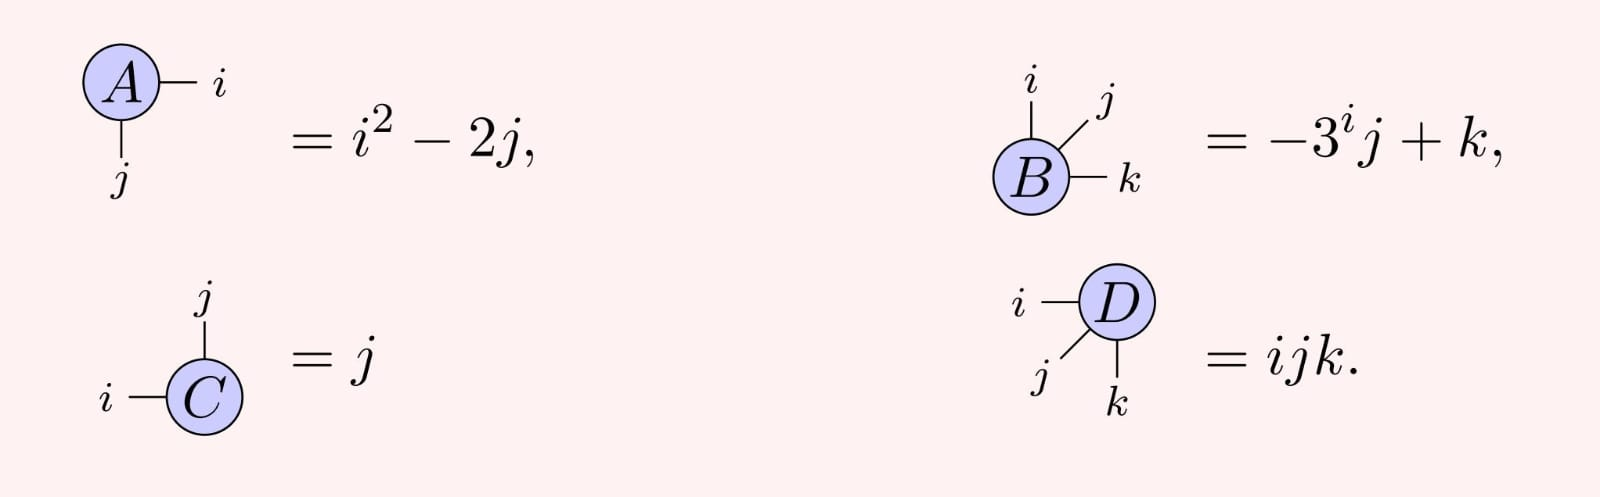
\includegraphics[width=0.6\linewidth]{images/tensorq1-1.jpeg}%
    \caption{Definitions of $A$, $B$, $C$ and $D$, Eqs.\eqref{def}}%
\end{figure}%

Calculate the value of the tensor network of Eq.~(1.22).

\begin{figure}[H]\centering
    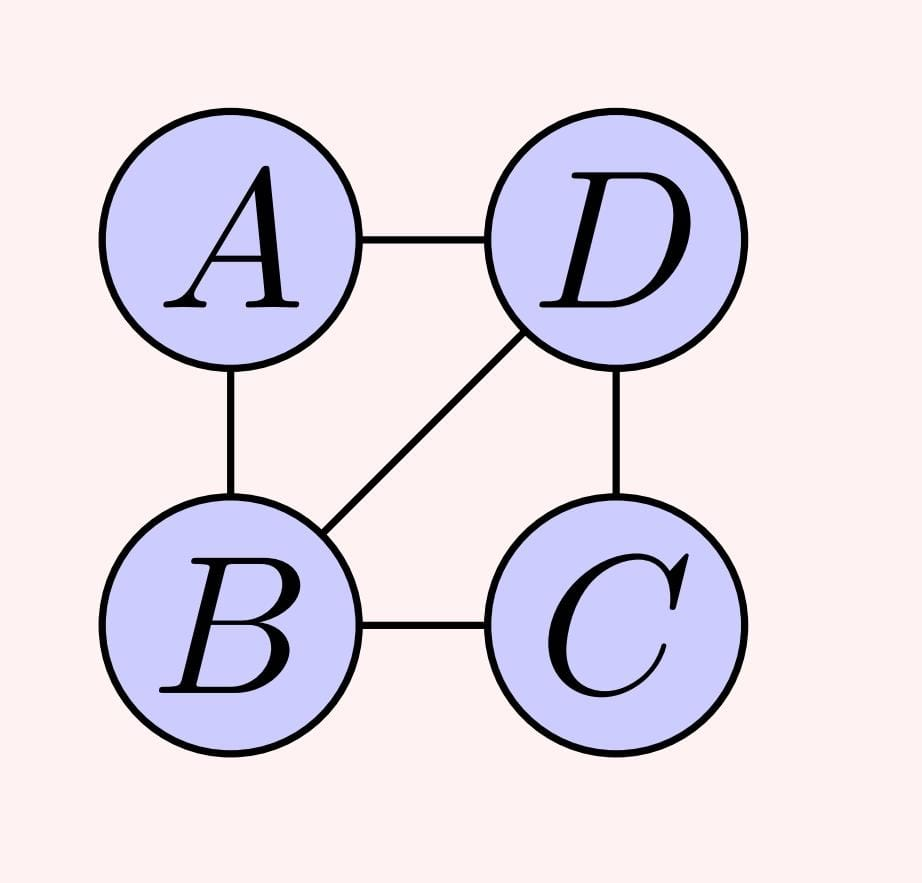
\includegraphics[width=0.25\linewidth]{images/tensorq1-2.jpeg}%
    \caption{The network to be contracted, Eq.~(1.22).}%
\end{figure}
\end{problem}


% ============================================================== solutions ===

\begin{solution}
There is no free index, so this is a scalar (the number of lines equal the number of indexed summed and must be consistent with the ordering $A_{i,j}, B_{i,j,k}$ to differentiate weach element of the tensor)
\begin{equation}
\begin{split}
     T &= \sum_{a,b,c,d,e} A_{a,b}B_{b,c,d}C_{d,e}D_{a,c,e}\\
     &= \sum_{a,b,c,d,e=0}^{2} (a^2  -2b)(-3^bc+d)(e)(ace)\\
     &= 1080
\end{split}
\end{equation}


\end{solution}


\attempt{
  date        = 2026-09-14,
  time        = 5min,
  difficulty  = 1,
  how it went = ,
}

\end{entry}
\begin{entry}{Q012}{Bubbling a network into a contraction table}

\entrymeta{
  topic   = {Tensor networks; contraction sequences; bubbling.},
  est     = $\sim$10 minutes,
  origin  = {Sourced. The original exercise; the worked example is reproduced so the
    required table format is unambiguous.},
  source  = {J.~C. Bridgeman and C.~T. Chubb, \emph{Hand-waving and Interpretive Dance:
    An Introductory Course on Tensor Networks}, J.~Phys.~A \textbf{50}, 223001 (2017),
    \href{https://arxiv.org/abs/1603.03039}{arXiv:1603.03039}, Section~1.6,
    Problem~2.},
  prereq  = {Section 1.4 (bubbling).},
  status  = open,
}

\begin{problem}
When a contraction is actually coded up, one contracts the tensors in one at a time and
must track, at each step, the open indices of the object built so far, the tensor being
absorbed, which indices are summed over in that step, and which new open indices the
incoming tensor contributes.

\begin{figure}[H]\centering
    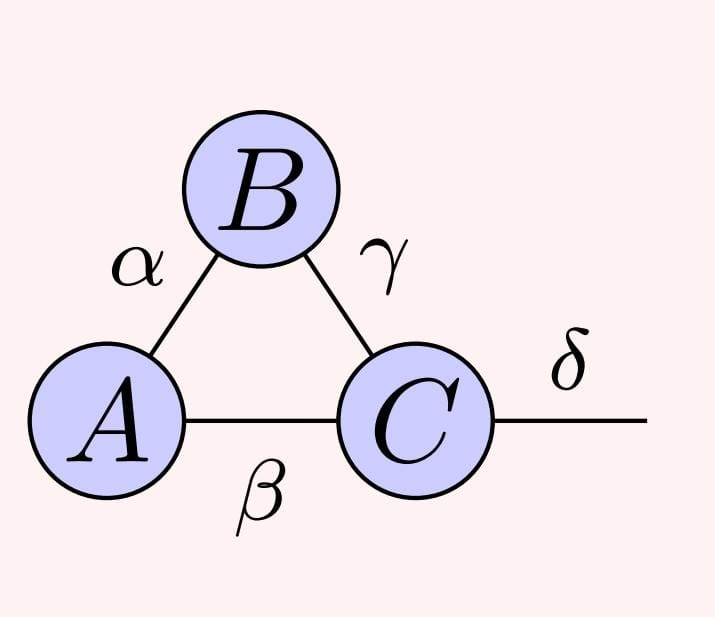
\includegraphics[width=0.2\linewidth]{images/tensorq2-1.jpeg}%
    \caption{The network of Eq.~(1.23), to be bubbled in alphabetical order.}%
\end{figure}


As an example, take the network of Eq.~(1.23): three tensors $A,B,C$ with bonds
$\alpha$ joining $A$ and $B$, $\beta$ joining $A$ and $C$, $\gamma$ joining $B$ and $C$,
and a free leg $\delta$ on $C$. Bubbling in alphabetical order gives


\begin{center}
\begin{tabular}{|c|c|c|c|}
\hline
Current & Tensor & Contract & New \\
\hline
--             & $A$ & --             & $\alpha,\beta$ \\
$\alpha,\beta$ & $B$ & $\alpha$       & $\gamma$ \\
$\beta,\gamma$ & $C$ & $\beta,\gamma$ & $\delta$ \\
\hline
\end{tabular}
\end{center}

Construct the corresponding table for the network of Eq.~(1.24), again bubbling in
alphabetical order.

\begin{figure}[H]\centering
    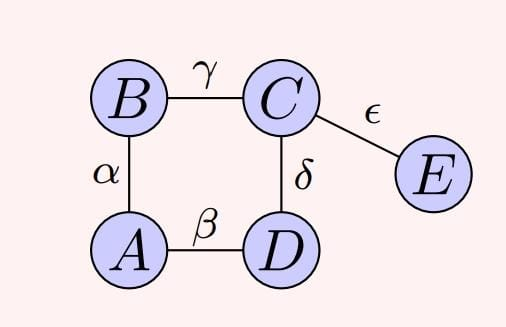
\includegraphics[width=0.2\linewidth]{images/tensorq2-2.jpeg}%
    \caption{The network of Eq.~(1.24), to be bubbled in alphabetical order}%
\end{figure}

and state the largest rank reached by the intermediate object, and whether a different
bubbling order would reduce it.

\end{problem}

% ============================================================== solutions ===

\begin{solution}
.
\vspace{0.1cm}
\begin{center}
\begin{tabular}{|c|c|c|c|}
\hline
Current & Tensor & Contract & New \\
\hline
--                      & $A$ & --          & $\alpha,\beta$ \\
  $\alpha,\beta$        & $B$ & $\alpha$    & $\gamma$   \\
 $\beta,\gamma$         & $C$ &  $\gamma$   &  $\delta,\epsilon$ \\
$\beta,\delta,\epsilon$ & $D$ &   $\delta,\beta$  & -- \\
            $\epsilon$  & $E$ &   $\epsilon$      &  -- \\
\hline
\end{tabular}
\end{center}
\vspace{0.1cm}
The largest rank is achieved after adding the tensor $C$ ($-A-B-C=$), where in this intermediate step we have a $\rank=3$ tensor. We could reduce the highest intermediate rank by starting from $E$, then going to $C$, we would contract $\epsilon$ and the intermediate tensor would be $\rank=2$, then, we can follow the adjacent $\rank=2$ tensors in the orders $B,A,D$ or $D,A,B$, on both cases at least one index is contracted and at most one is added, keeping the $\rank$ always lower or equal to $2$.
\end{solution}



\attempt{
  date        = 2026-09-14,
  time        = 10min,
  difficulty  = 1,
  how it went = ,
}

\end{entry}

\daysession{9}{2026-09-15}
\begin{entry}{Q013}{Counting colourings with tensor networks}

\entrymeta{
  topic   = {Tensor networks; graph colouring; counting complexity.},
  est     = $\sim$30 minutes total --- longer than the usual daily entry.
    Part (a) alone is $\sim$12 minutes and is the core; (b) and (c) may be done
    in a second sitting.,
  origin  = {Sourced. The original exercise; the definitions of $e$ and $n$ from
    Section~1.5 are inlined so the statement stands alone.},
  source  = {J.~C. Bridgeman and C.~T. Chubb, \emph{Hand-waving and Interpretive Dance:
    An Introductory Course on Tensor Networks}, J.~Phys.~A \textbf{50}, 223001 (2017),
    \href{https://arxiv.org/abs/1603.03039}{arXiv:1603.03039}, Section~1.6,
    Problem~3.},
  prereq  = {Section 1.5 (computational complexity).},
  status  = open,
}

\begin{problem}
Recall the two binary tensors of Section~1.5. The tensor $e$ takes the value $1$ if and
only if all of its indices are equal, and $0$ otherwise; the tensor $n$ takes the value
$1$ if and only if all of its indices differ, and $0$ otherwise. Given an arbitrary
graph, build a tensor network by placing an $e$ tensor at each vertex and an $n$ tensor
in the middle of each edge, inheriting the connectivity of the graph, as in
Eq.~(1.19).

\begin{figure}[H]\centering
    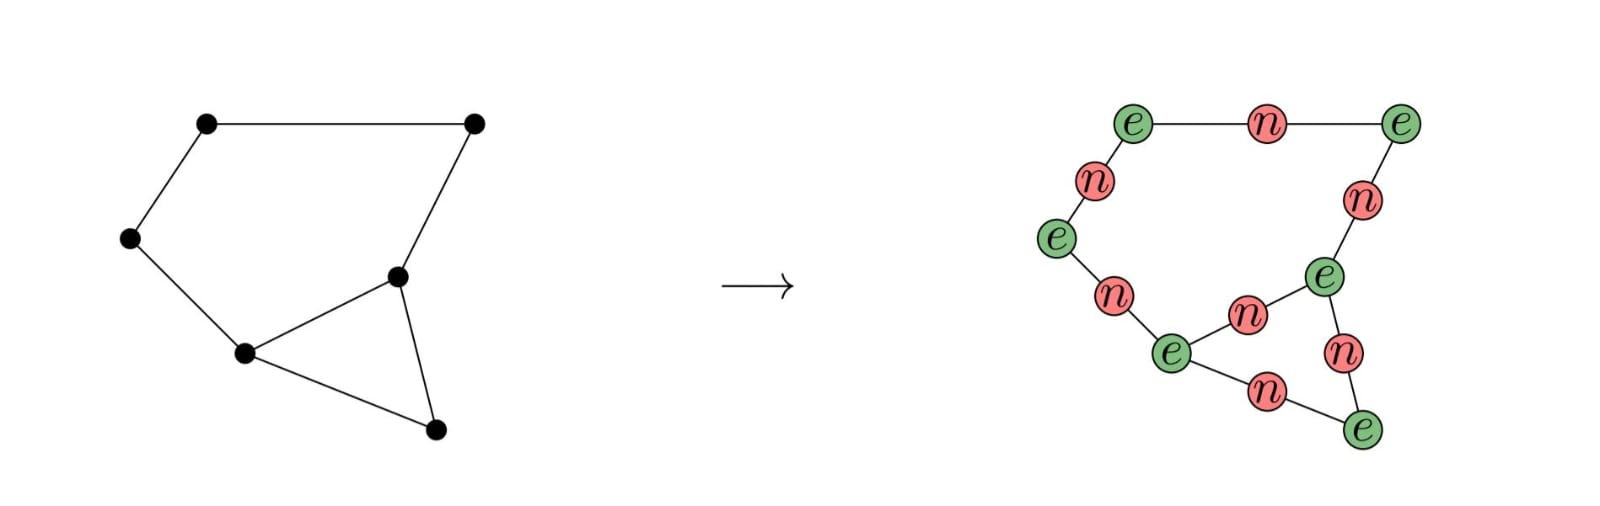
\includegraphics[width=0.7\linewidth]{images/tensorq3-1.jpeg}%
    \caption{The graph of Eq.~(1.19) and the tensor network built from it.}%
\end{figure}%

With $q$-dimensional indices, the nonzero contributions to this network are exactly the
vertex $q$-colourings of the graph, so its contraction counts them.

\begin{enumerate}[label=\textbf{(\alph*)},leftmargin=*]
  \item Calculate the contraction of the network of Eq.~(1.19) for bond dimension $q$,
        i.e.\ the number of three-colourings of the corresponding graph.
  \item Using the $e$ and $n$ tensors, construct a tensor network whose contraction gives
        the number of \emph{edge} colourings. For a planar graph, construct an analogous
        network counting \emph{face} colourings.
\end{enumerate}


\end{problem}

% ============================================================== solutions ===

\begin{solution}[Part (a)]
The equivalent tensor of e connected to two n, is
\begin{equation}
\begin{split}
    x_{a,b} &= \sum_{i,j}n_{a,i}e_{i,j}n_{j,b}\\
    &= \sum_{i,j} (1-\delta_{a,i})\delta_{i,j}(1-\delta_{j,b})\\
    &= \sum_{i} (1-\delta_{a,i})(1-\delta_{i,b})\\
    &= \delta_{a,b} + (q-2)
\end{split} 
\end{equation}

% requires \usepackage{tikz}
\usetikzlibrary{fit}
% requires \usetikzlibrary{fit}
\begin{figure}[H]\centering
\resizebox{\linewidth}{!}{%
\begin{tikzpicture}[
  every node/.style={font=\footnotesize},
  ten/.style={circle,draw,minimum size=5.5mm,inner sep=0pt},
  blu/.style={ten,fill=blue!20},
  red/.style={ten,fill=red!35},
  yel/.style={ten,fill=yellow!55},
  grn/.style={ten,fill=green!35},
  cut/.style={draw,dashed,thick,rounded corners,inner sep=3pt},
]

%=================== PANEL 1 : original, relaid out ===================
\begin{scope}[shift={(0,0)}]
  % upper branch: v5 - v3 - v1 - v2 - v4
  \node[blu] (v1) at (2.0, 2.6) {$e$};
  \node[blu] (nb) at (1.2, 2.3) {$n$};
  \node[blu] (v3) at (0.4, 2.0) {$e$};
  \node[blu] (nc) at (0.2, 1.0) {$n$};
  \node[blu] (na) at (2.8, 2.3) {$n$};
  \node[blu] (v2) at (3.6, 2.0) {$e$};
  \node[blu] (nd) at (3.8, 1.0) {$n$};
  % axis
  \node[blu] (v5) at (0.0, 0.0) {$e$};
  \node[blu] (nn) at (2.0, 0.0) {$n$};
  \node[blu] (v4) at (4.0, 0.0) {$e$};
  % lower branch: v5 - v6 - v4
  \node[blu] (nf) at (1.2,-1.5) {$n$};
  \node[blu] (v6) at (2.0,-1.9) {$e$};
  \node[blu] (ng) at (2.8,-1.5) {$n$};

  \draw (v5)--(nc)--(v3)--(nb)--(v1)--(na)--(v2)--(nd)--(v4);
  \draw (v5)--(nn)--(v4);
  \draw (v5) to[bend right=12] (nf);
  \draw (nf)--(v6)--(ng);
  \draw (ng) to[bend right=12] (v4);

  \node[cut,red!80!black,fit=(nc)(v3)(nb)] {};
  \node[cut,red!80!black,fit=(na)(v2)(nd)] {};
  \node[cut,red!80!black,fit=(nf)(v6)(ng)] {};
\end{scope}

\node at (5.1,0.3) {\Large$\to$};

%=================== PANEL 2 : after x-reduction ===================
\begin{scope}[shift={(6.0,0)}]
  \node[blu] (w1) at (2.0, 2.3) {$e$};
  \node[red] (x2) at (0.7, 1.5) {$x$};
  \node[red] (x1) at (3.3, 1.5) {$x$};
  \node[blu] (w5) at (0.0, 0.0) {$e$};
  \node[blu] (nn) at (2.0, 0.0) {$n$};
  \node[blu] (w4) at (4.0, 0.0) {$e$};
  \node[red] (x3) at (2.0,-1.5) {$x$};

  \draw (w5)--(x2)--(w1)--(x1)--(w4);
  \draw (w5)--(nn)--(w4);
  \draw (w5) to[bend right=15] (x3);
  \draw (x3) to[bend right=15] (w4);

  \node[cut,yellow!60!black,fit=(x2)(w1)(x1)] {};
  \node[cut,green!50!black,fit=(w5)(nn)(x3)(w4)] {};
\end{scope}

\node at (11.1,0.3) {\Large$\to$};

%=================== PANEL 3 : y over z ===================
\begin{scope}[shift={(11.9,0)}]
  \node[yel] (y) at (0.9, 1.3) {$y$};
  \node[grn] (z) at (0.9,-0.6) {$z$};
  \draw (y) to[bend left=38]  (z);
  \draw (y) to[bend right=38] (z);
  \node[cut,gray,fit=(y)(z)] {};
\end{scope}

\node at (13.9,0.3) {\Large$\to$};

%=================== PANEL 4 : scalar ===================
\begin{scope}[shift={(14.5,0)}]
  \node[ten,fill=gray!40] at (0.5,0.3) {};
\end{scope}

\end{tikzpicture}}
\caption{Contraction of the network of Eq.~(1.19), redrawn so that the three
$n$--$e$--$n$ chains occupy disjoint regions. Red contours mark the chains replaced by
$x$; the yellow contour is $x$--$e$--$x\to y$; the green contour is the pair of vertices
joined by the parallel $n$ and $x$ bonds, $\to z$. Contracting $y$ against $z$ across the
double bond leaves a scalar.}
\end{figure}%

The upper part inside the yellow dashed line is equivalent to 
\begin{equation}
\begin{split}
    y_{a,b}&= \sum_{i,j}x_{a,i}e_{i,j}x_{j,b}\\
    &=\sum_{i,j} x_{a,i}\delta_{i,j}x_{j,b}\\
    &= \sum_{i} x_{a,i}x_{i,b}\\
    &= \sum_i (q-2)^2 + (q-2)(\delta_{a,i}+\delta_{i,b}) + \delta_{a,i}\delta_{i,b}\\
    &= q(q-2)^2+ 2(q-2) + \delta_{a,b}
\end{split}
\end{equation}
whereas for the below part inside the green dashed line is equivalent to 

\begin{equation}
\begin{split}
    z_{a,b}&= \sum_{i,j,k,l}e_{a,i,j}x_{j,l}n_{i,k}e_{k,l,b}\\
    &=\sum_{i,j,k,l}\delta_{a,i,j}x_{j,l}n_{i,k}\delta_{k,l,b}\\
    &= x_{a,b}n_{a,b}
\end{split}
\end{equation}
so
\begin{equation}
\begin{split}
    T&=\sum_{a,b} z_{a,b}y_{a,b}\\
    &= \sum_{a,b} (q(q-2)^2+ 2(q-2) + \delta_{a,b})((q-2)+\delta_{a,b})(1-\delta_{a,b})\\
    &= q(q-1)(q-2)^2[q^2-2q+2]
\end{split}
\end{equation}


\end{solution}

\begin{solution}[Part (b)]
These tensor $e$ and $n$ allows one to generalize the q-colouring counting problem by simple using $e$ in place of the counting object and $n$ used as the "adjacency mediator"  forcing that no adjacent objects have the same colour. To count the number of edges colouring you may draw a tensor network with $e$ in the edges and $n$ in the vertices, meanwhile to count the number of face colouring you draw a network with $e$ in the face( inside each polygon) and $n$ in the commom edges of the polygons. 
\end{solution}





\attempt{
  date        = ,
  time        = ,
  difficulty  = ,
  how it went = ,
}

\end{entry}

\daysession{10}{2026-09-17}
\begin{entry}{Q014}{Grassmann integrals and the trace of a Floquet operator}

\entrymeta{
  topic   = {Grassmann (Berezin) integration; Gaussian fermionic integrals;
    field-theory approach to quantum chaos.},
  est     = $\sim$25 minutes --- longer than the usual daily entry; part (c) is the core
    and may be done separately.,
  origin  = {Adapted. Reconstructed from a lecture exercise; the Grassmann axioms are
    inlined and the time-lattice conventions fixed so the statement is self-contained.},
  source  = {T. Micklitz, lectures on \emph{Field-Theory Approach to Quantum Chaos},
    School on Analytical and Numerical Methods for Disordered Quantum Systems.},
  prereq  = {None beyond linear algebra; all Grassmann conventions are stated below.},
  status  = open,
}

\begin{problem}
\textbf{Conventions.} Let $\psi_1,\dots,\psi_n,\bar\psi_1,\dots,\bar\psi_n$ be
\emph{Grassmann variables}: generators of an associative algebra over $\CC$ subject to
\[
  \{\psi_i,\psi_j\}=\{\bar\psi_i,\bar\psi_j\}=\{\psi_i,\bar\psi_j\}=0
  \qquad\text{for all } i,j,
\]
so in particular $\psi_i^{2}=\bar\psi_i^{2}=0$. Every function of them is a polynomial
of degree at most one in each generator. \emph{Berezin integration} in a single variable
is the linear map defined by
\begin{equation}
    \int d\psi\;1=0,
  \qquad
  \int d\psi\;\psi=1,
  \label{grassman identity}
\end{equation}

and the differentials $d\psi_i,d\bar\psi_i$ anticommute with each other and with all
generators. For $n$ pairs write
\[
  D(\bar\psi,\psi):=\prod_{i=1}^{n} d\bar\psi_i\, d\psi_i ,
  \qquad\text{normalised so that}\qquad
  \int D(\bar\psi,\psi)\;\prod_{i=1}^{n}\psi_i\bar\psi_i \;=\;1 .
\]
For $A\in\CC^{n\times n}$ set $\bar\psi A\psi:=\sum_{i,j}\bar\psi_i A_{ij}\psi_j$.

\begin{enumerate}[label=\textbf{(\alph*)},leftmargin=*]
  \item Prove that
        \[
          \int D(\bar\psi,\psi)\; e^{-\bar\psi A\psi} \;=\;\det A .
        \]
  \item Prove that, for $A$ invertible,
        \[
          \int D(\bar\psi,\psi)\; e^{-\bar\psi A\psi}\,\psi_a\bar\psi_b
          \;=\;\det A\;\bigl(A^{-1}\bigr)_{ab} .
        \]
  \item Let $U_0$ be a unitary on $\CC^{N}$ (one step of a Floquet evolution), and let
        the discrete time lattice be $\{0,1,\dots,t\}$, on which the lowering operator
        $T_-$ acts by $T_-\ket{\tau}=\ket{\tau-1}$, i.e.
        $(T_-)_{\tau,\tau'}=\delta_{\tau,\tau'-1}$. Take Grassmann variables
        $\psi_{(i,\tau)},\bar\psi_{(i,\tau)}$ indexed by $i\in\{1,\dots,N\}$ and
        $\tau\in\{0,\dots,t\}$, and set
        \[
          A=\id-U_0\otimes T_- .
        \]
        Show that $\det A=1$, compute $\bigl(A^{-1}\bigr)_{(i,\tau),(j,\tau')}$, and
        conclude that
        \[
          \int D(\bar\psi,\psi)\; e^{-\bar\psi A\psi}
          \sum_{a=1}^{N}\psi_{(a,0)}\,\bar\psi_{(a,t)}
          \;=\;\Tr\bigl(U_0^{\,t}\bigr).
        \]
        Explain why an insertion diagonal in the time index, $\sum_a
        \psi_{(a,\tau)}\bar\psi_{(a,\tau)}$, cannot produce this result.
\end{enumerate}
\end{problem}

% ============================================================== solutions ===

\begin{solution}[Part (a)]
Since $\psi_i^{2}=\bar\psi_i^{2}=0$, we have that 
\begin{equation}
    e^{-\bar\psi A\psi}= \prod_{i,j}(1 -  \bar\psi_i A_{ij}\psi_j)=O(0)+O(2)+...+O(2n)
\end{equation}
where here $O(2k)$ represent the term where there is a product of $2k$ Grassmann variables, i.e.,
\begin{equation*}
\begin{split}
    O(2k)= (-1)^k\sum_{\substack{i_1\neq...\neq i_k\\j_1\neq...\neq j_k}} \prod_{x=1}^{k}\bar\psi_{i_x}A_{i_x,j_x}\psi_{j_x}
\end{split}
\end{equation*}
(notice that equal index leads to 0 contribution, $\psi_i^{2}=\bar\psi_i^{2}=0$ forcing the summation to be over different index) but from \eqref{grassman identity}, any term that doesn't have the full $2n$ Grassmann variables vanishes when integrated, $\int D(\bar\psi,\psi) O(2k)=0,\ k<n$, then 
\begin{equation}
\begin{split}
    \int D(\bar\psi,\psi)\; e^{-\bar\psi A\psi} = \int D(\bar\psi,\psi) \sum_{\substack{i_1\neq...\neq i_n\\j_1\neq...\neq j_n}} \prod_{x=1}^{n}\bar\psi_{i_x}A_{i_x,j_x}\psi_{j_x}
\end{split}
\end{equation}
which can be rewritten in the permutation notation 
\begin{equation}
\begin{split}
    \int D(\bar\psi,\psi)\; e^{-\bar\psi A\psi} =& (-1)^n\int D(\bar\psi,\psi) \sum_{\sigma \in S_n} \prod_i^n \bar\psi_i A_{i\sigma(i)}\psi_{\sigma(i)}\\
    =& (-1)^n\sum_{\sigma \in S_n}\int D(\bar\psi,\psi)\prod_i\bar\psi_i \psi_{\sigma(i)}A_{i \sigma(i)}.
\end{split}
\end{equation}
Now, due to the anti-commutativity of the Grassmann variables, we can rewrite the normalization condition and then derive for a generic permutation
\begin{equation}
   \int D(\bar\psi,\psi)\prod_i\bar\psi_i \psi_{i} =(-1)^n\implies\int D(\bar\psi,\psi)\prod_i\bar\psi_i \psi_{\sigma(i)}=(-1)^n\text{sign}(\sigma)
\end{equation}, where an even permutation would require an even number of exchanges to order the integral as products $\int d \psi \psi$, meanwhile an odd permutation requires an odd number of exchanges, leading to a $-$ sign overall, hence
\begin{equation}
\begin{split}
    \int D(\bar\psi,\psi)\; e^{-\bar\psi A\psi}
    =&\sum_{\sigma \in S_n}\text{sign}(\sigma)\prod_iA_{i \sigma(i)}\\
    =& \det (A
)\end{split}
\end{equation}
\end{solution}

\begin{solution}[Part (b)]
We can see the matrix itself as a list of complex variables, consider Einstein summation notation for an Euclidean norm, such that the expression can be written as (for the sake of precision consider $X_{i,j}$ the list of complex variables)
\begin{equation}
\begin{split}
    \int D(\bar\psi,\psi)\; e^{-\bar\psi A\psi}\psi_a \bar\psi_b
    =&\int D(\bar\psi,\psi)\; e^{-\bar\psi^\nu A_{\nu\mu}\psi^\mu}\psi_a \bar\psi_b\\
    =& \int D(\bar\psi,\psi)\; e^{-\bar\psi^\nu A_{\nu\mu}\psi^\mu}(-\bar\psi_b \psi_a) \\
    =&\bigg(\frac{\partial}{\partial X_{ba}}\int D(\bar\psi,\psi)\; e^{-\bar\psi^\nu X_{\nu\mu}\psi^\mu}\bigg)_{X=A}\\
    =& \bigg(\frac{\partial}{\partial X_{ba}}\det(X)\bigg)_{X=A}
\end{split}
\end{equation}
From Cramer's rule for the determinant, for any row $i$
\begin{equation*}
    \det X = \sum_{j}X_{ij}C_{ij}
\end{equation*}
where $C_{ij}$ is the cofactor in the corresponding position $i,j$, which depends on all variables of $X$ besides the ones that have either row $i$ or column $j$ (you eliminate the row $i$ and columns $j$ to calculate the determinant of the remaining matrix, to attain $C_{i,j}$), so taking the row $i=b$, we can write $\det X = \sum_{j}X_{bj}C_{bj}$. No element of the summation depends on $X_{ba}$ besides when $j=a$, so
\begin{equation*}
    \frac{\partial}{\partial X_{ba}}\det X = C_{ba}
\end{equation*}
Now, from Laplace's formula for the inverse, or cofactor method, the inverse is calculated precisely from the cofactor by
$$(X^{-1})_{ij} =\frac{C_{ji} }{\det X}$$
therefore
\begin{equation}
    \int D(\bar\psi,\psi)\; e^{-\bar\psi A\psi}\psi_a \bar\psi_b
    = \det A (A^{-1})_{ab}
\end{equation}
\end{solution}

\begin{solution}[Part (c)]
Defining properly the notation for the spatial and temporal degrees of freedom
\begin{equation}
\begin{split}
    \sum_{a,a',\tau,\tau'} \bar \psi_{(a,\tau)} (U^k_0\otimes T_-^k)_{(a,a'),(\tau,\tau')} \psi_{(a',\tau')}= \sum_{a,a',\tau,\tau'} \bar \psi_{(a,\tau)} (U^k_0)_{(a,a')}\otimes (T_-^k)_{(\tau,\tau')} \psi_{(a',\tau')}
\end{split}
\end{equation}
Now notice 
\begin{equation}
    T_-=\sum_{\tau=1}^{t}\ket{\tau-1}\bra{\tau}
=\begin{pmatrix}
0 & 1 & 0 & \cdots & 0 \\
0 & 0 & 1 & \ddots & \vdots \\
\vdots & \vdots & \ddots & \ddots & 0 \\
0 & 0 & \cdots & 0 & 1 \\
0 & 0 & \cdots & 0 & 0 \qquad 
\end{pmatrix},
\qquad
(T_-)_{\tau\tau'}=\delta_{\tau,\tau'-1}. \qquad \text{odering}\ \ket{0} = \begin{pmatrix}
    1\\
    ...\\
    0
\end{pmatrix}
\end{equation}
exponentiation of $T_-$ lower its own entries, leading to
\begin{equation}
T_-^{\,k}=\sum_{\tau=1}^{t}\ket{\tau-1}\bra{\tau}
=\begin{pmatrix}
0_{(t+1-k)\times k} & \id_{t+1-k} \\[2pt]
0_{k\times k} & 0_{k\times(t+1-k)}
\end{pmatrix},
\quad (T_-^{\,k})_{\tau\tau'}=\delta_{\tau,\tau'-k},,
\qquad T_-^{\,t+1}=0 ,
\end{equation}
Moreover, we have that $(T_-^k)_{0t} = \delta_{kt}$, which means that the we got apply the $T_-$ $t$ times in order to have an element in the last columns of the first row, meanwhile the condition $T_{-}^{t+1}=0$, makes $U_0\otimes T_-$ nilpotent, such that the inverse of $A=\id-U_0\otimes T_-$ can be calculated from the geometric series, 
\begin{equation}
    (\id -U_0\otimes T_-)^{-1}= \sum_{k=0}^t U_0^k \otimes T_{-}^k
\end{equation}
 thus
\begin{equation}
    (A^{-1})_{(a,0),(b,t)}= (U_0^t)_{a,b}
\end{equation}
Finally,
\begin{equation}
    A=\id-U_0\otimes T_-=
\begin{pmatrix}
\id_N & -U_0 & & & \\
 & \id_N & -U_0 & & \\
 & & \ddots & \ddots & \\
 & & & \id_N & -U_0 \\
 & & & & \id_N
\end{pmatrix}
\end{equation} such that $\det A=1$, therefore, using item b) 
\begin{equation}
    \int D(\bar\psi,\psi)\; e^{-\bar\psi A\psi}
          \sum_{a=1}^{N}\psi_{(a,0)}\,\bar\psi_{(a,t)}
          \;=\; \sum_a =\Tr\bigl(U_0^{\,t}\bigr).
\end{equation}
 



\end{solution}



\attempt{
  date        = 2026-09-15,
  time        = ,
  difficulty  = ,
  how it went = ,
}

\end{entry}
\begin{entry}{Q015}{From free to damped: the arc propagator at finite $\gamma$}

\entrymeta{
  topic   = {Discrete-time field theory; contour times; finite-difference Green
    functions; quantum chaos.},
  est     = $\sim$15 minutes,
  origin  = {Adapted. Reconstructed from a lecture exercise; the index conventions,
    the Heaviside convention and the structural part (a) are inlined so the statement
    stands alone.},
  source  = {T. Micklitz, lectures on \emph{Field-Theory Approach to Quantum Chaos},
    School on Analytical and Numerical Methods for Disordered Quantum Systems.
    Companion to \qref{Q016}.},
  prereq  = {None beyond finite differences.},
  status  = open,
}

\begin{problem}
\textbf{What this describes.} In the field theory of the previous entry, the object of
interest is not a single amplitude but a \emph{pair} of them: one propagating forward in
time and one backward, whose phases cancel and which therefore survive an average over
the random dynamics. The propagator $\Pi$ follows such a pair, and each of its legs
carries two times, one on each branch. The free theory has no scale: once formed, a pair
stays correlated forever. The interacting theory has one, $\gamma$, at which the two
branches lose their correlation; the exercise is to see that scale appear, and to see
what it means.

\textbf{Conventions.} Time is discrete, $n\in\ZZ$. Each leg carries a pair of contour
times $(n^{+},n^{-})$, forward and backward. Write the pair as a single label,
\[
  \mathbf n:=(n^{+},n^{-}),
  \qquad
  \Delta n:=n^{+}-n^{-}\ \ \text{(relative time)},
  \qquad
  \bar n:=\tfrac12\bigl(n^{+}+n^{-}\bigr)\ \ \text{(mean time)} ,
\]
so that $\mathbf n\mapsto(\Delta n,\bar n)$ is a change of coordinates on the set of
pairs: $\Delta n$ records how far apart on the two branches the pair sits, and $\bar n$
how far along both have travelled together.

The propagator $\Pi_{\mathbf n_2,\mathbf n_1}$ is a kernel from the incoming pair
$\mathbf n_1$ to the outgoing pair $\mathbf n_2$. Kernels compose by summation over the
repeated pair,
\[
  (KL)_{\mathbf n_2,\mathbf n_1}
  :=\sum_{\mathbf m}K_{\mathbf n_2,\mathbf m}\,L_{\mathbf m,\mathbf n_1},
  \qquad
  \bigl(\id\bigr)_{\mathbf n_2,\mathbf n_1}
  =\delta_{n_2^{+},n_1^{+}}\,\delta_{n_2^{-},n_1^{-}} ,
\]
and act on the outgoing label only. Let $T$ be the kernel that advances \emph{both}
contour times by one unit --- one step of the dynamics, applied to both branches at
once,
\[
  T_{\mathbf n,\mathbf m}
  :=\delta_{n^{+},\,m^{+}+1}\;\delta_{n^{-},\,m^{-}+1},
\]
and set $d:=\id-T$, the discrete counterpart of a time derivative. Write $\Theta(u)=1$
for $u\ge0$ and $\Theta(u)=0$ for $u<0$, so that $\Pi$ is supported on outgoing times
later than incoming ones. Finally let $D_0>0$ be the normalisation constant of the notes
and $\gamma>0$ a damping rate.

\begin{enumerate}[label=\textbf{(\alph*)},leftmargin=*]
  \item Show that $T$ preserves the relative time and lowers the mean time by one:
        in the coordinates $(\Delta n,\bar n)$,
        \[
          T_{\mathbf n,\mathbf m}
          =\delta_{\Delta n,\Delta m}\;\delta_{\bar n,\,\bar m-1}.
        \]
        Deduce that if $K_{\mathbf n_2,\mathbf n_1}
        =\delta_{\Delta n_2,\Delta n_1}\,f(\bar n_2-\bar n_1)$ for some
        $f:\ZZ\to\CC$, then
        \[
          (dK)_{\mathbf n_2,\mathbf n_1}
          =\delta_{\Delta n_2,\Delta n_1}\bigl[f(u)-f(u-1)\bigr],
          \qquad u:=\bar n_2-\bar n_1 ,
        \]
        so that the problem reduces to a one-dimensional recursion in $u$.

  \item \emph{Free theory.} Verify that the propagator for the free theory
        \[
          \Pi_{\mathbf n_2,\mathbf n_1}
          =\frac{1}{D_0}\,\delta_{\Delta n_2,\Delta n_1}\,\Theta(\bar n_2-\bar n_1)
        \]
        satisfies
        \[
          (d\,\Pi)_{\mathbf n_2,\mathbf n_1}
          =\frac{1}{D_0}\,\delta_{\Delta n_2,\Delta n_1}\,
            \delta_{\bar n_2,\bar n_1} .
        \]

  \item \emph{Interacting theory.} The propagator for the interacting theory (with mass) is
        \[
          \Pi^{\mathrm{arc}}_{\mathbf n_2,\mathbf n_1}
          =\frac{1}{D_0}\,\delta_{\Delta n_2,\Delta n_1}\,
            \frac{\Theta(\bar n_2-\bar n_1)}{(1+\gamma)^{\,\bar n_2-\bar n_1+1}} .
        \]
        Show that 
        \[
          \bigl[(d+\gamma)\,\Pi^{\mathrm{arc}}\bigr]_{\mathbf n_2,\mathbf n_1}
          =\frac{1}{D_0}\,\delta_{\Delta n_2,\Delta n_1}\,
            \delta_{\bar n_2,\bar n_1} ,
        \]
        i.e.\ $\Pi^{\mathrm{arc}}$ is the Green function of $d+\gamma$ with the same
        right-hand side as in the free case. Note where the factor
        $(1+\gamma)^{-u}$ disappears from the final answer.

   \item \emph{The lattice scale.} Fix the relative time and compare successive mean
        times: show that for $\bar n_2\ge\bar n_1$ the ratio
        \[
          \frac{\Pi^{\mathrm{arc}}_{\,(\Delta n,\,\bar n_2+1),\,\mathbf n_1}}
               {\Pi^{\mathrm{arc}}_{\,(\Delta n,\,\bar n_2),\,\mathbf n_1}}
        \]
        does not depend on $\bar n_2$, and identify it. The decay is therefore
        geometric: the same fraction of the amplitude is lost at every step, regardless
        of how long the pair has already survived.

        Explain why this is the expected structure rather than a coincidence, by reading
        it off the equation $\Pi^{\mathrm{arc}}=\bigl[(1+\gamma)\id-T\bigr]^{-1}$ that
        (c) establishes: each application of $T$ advances both branches by one step of
        the dynamics, and each such step is accompanied by the same factor. What
        property of the underlying dynamics does this memorylessness reflect, and what
        would have to change for the loss per step to depend on $\bar n_2-\bar n_1$?


  \item \emph{The approximation.} Show that $(1+\gamma)^{-u}=e^{-\gamma u}$ up to a
        relative error controlled by $\gamma^{2}u$, and say why it is this product,
        rather than $\gamma$ alone, that must be small for the exponential form to hold. Determine also the sign of
        the discrepancy: does the lattice decay faster or slower than the exponential?

  \item \emph{The continuum limit.} Take as given that the Green function of
        $\partial_{\mathcal T}+\Gamma$ is $\Theta(\mathcal T)\,e^{-\Gamma\mathcal T}$,
        where the constant $\Gamma$ added to a first-order derivative is a \emph{mass
        term} and fixes the only scale of the continuum theory, $\tau=1/\Gamma$. Let
        $\delta t$ be the physical duration of one lattice step, so that
        $\mathcal T=u\,\delta t$ and $\gamma=\Gamma\,\delta t$. Using~(e), show that
        $\Pi^{\mathrm{arc}}$ converges to the continuum Green function as
        $\delta t\to0$, and state precisely which quantity is held fixed in the limit
        and which is sent to zero. Explain why the limit cannot be taken at fixed $u$,
        nor at fixed $\gamma$, and why the physically meaningful statement is that
        $\delta t$ disappears from the answer while $\tau$ does not: the scale belongs
        to the theory, the lattice spacing to its description. How many lattice steps
        does one lifetime $\tau$ contain, and what does that number have to be for the
        continuum description to apply?
\end{enumerate}
\end{problem}

% ============================================================== solutions ===

\begin{solution}[a]
$n^+=m^+ - 1$ and $n^-=m^- - 1$ if and only if $n^+ - n^- = m^+ - m^-$ and $\frac{n^+ + n^-}{2} =\frac{m^+ + m^-}{2} -1$, thus
\[
          T_{\mathbf n,\mathbf m}
          =\delta_{\Delta n,\Delta m}\;\delta_{\bar n,\,\bar m+1}.
        \]
Applying $T$ to such $K$
\begin{equation}
    \begin{split}
        (TK)_{\mathbf n_2, \mathbf n_1} &= \sum_{\mathbf m} T_{\mathbf n_2,\mathbf{ m}}K_{\mathbf{ m}, \mathbf n_1}\\
        &= \sum_{\Delta m, \bar m} \delta_{\Delta n_2,\Delta m}\;\delta_{\bar n_2,\,\bar m+1} \delta_{\Delta m,\Delta n_1}\,f(\bar m - \bar n_1) \\
        &=  \delta_{\Delta n_2,\Delta n_1}f(\bar n_2 -1 -n_1)\\
        &=  \delta_{\Delta n_2,\Delta n_1}f(u-1)
    \end{split}
\end{equation}
Therefore, it follows directly when applying $d$

\end{solution}

\begin{solution}[b]
From a)
\begin{equation}
   (d\,\Pi)_{\mathbf n_2,\mathbf n_1}
          =\frac{1}{D_0}\,\delta_{\Delta n_2,\Delta n_1}\,
            \big(\Theta({\bar n_2-\bar n_1}) - \Theta({\bar n_2-\bar n_1}-1)\big)
\end{equation}
Now if $\bar n_2-\bar n_1-1 \geq 0$, both $\Theta$ are equal to 1, leading to a null for the finite difference. If $\bar n_2-\bar n_1<0$, both vanish. So the finite difference only survives when $\bar n_2-\bar n_1 = 0$. Therefore,
\[
          (d\,\Pi)_{\mathbf n_2,\mathbf n_1}
          =\frac{1}{D_0}\,\delta_{\Delta n_2,\Delta n_1}\,
            \delta_{\bar n_2,\bar n_1} .
        \]
\end{solution}

\begin{solution}[c]
Applying item a) we get that 
\begin{equation}
  d \Pi^{\mathrm{arc}}_{\mathbf n_2,\mathbf n_1}
          =\frac{1}{D_0}\,\delta_{\Delta n_2,\Delta n_1}\,
            \left(\frac{\Theta(\bar n_2-\bar n_1)}{(1+\gamma)^{\,\bar n_2-\bar n_1+1}}-\frac{\Theta(\bar n_2-\bar n_1-1)}{(1+\gamma)^{\,\bar n_2-\bar n_1}} \right) .
\end{equation}
Meanwhile 
\begin{equation}
\begin{split}
    \gamma \Pi^{\mathrm{arc}}_{\mathbf n_2,\mathbf n_1}
          &=\frac{1}{D_0}\,\delta_{\Delta n_2,\Delta n_1}\,
            \frac{\Theta(\bar n_2-\bar n_1)}{(1+\gamma)^{\,\bar n_2-\bar n_1}}\left(\frac{\gamma}{1+\gamma} \right) \\
         &=\frac{1}{D_0}\,\delta_{\Delta n_2,\Delta n_1}\,
            \frac{\Theta(\bar n_2-\bar n_1)}{(1+\gamma)^{\,\bar n_2-\bar n_1}}\left(1-\frac{1}{1+\gamma} \right)  
\end{split}
\end{equation}
 To conclude, we must notice that after summing both expressions, the delta makes the only non-zero contribution occur when $\bar n_2 = \bar n_1$, reducing the exponent of the denominator to 0
 \begin{equation}
 \begin{split}
      (d+\gamma) \Pi^{\mathrm{arc}}_{\mathbf n_2,\mathbf n_1}
          &=\frac{1}{D_0}\,\delta_{\Delta n_2,\Delta n_1}\,
            \frac{\delta_{\bar n_2,\bar n_1}}{(1+\gamma)^{\,\bar n_2-\bar n_1}} \\
            &= \frac{1}{D_0}\,\delta_{\Delta n_2,\Delta n_1}\,
            \delta_{\bar n_2,\bar n_1} 
 \end{split}
 \end{equation}
This can be seen as the mass term for the theory
\end{solution}

\begin{solution}[d]
The ratio is given by 
\begin{equation*}
        (1+\gamma)^{-1}
\end{equation*}
which is smaller than $1$, reflecting the expected damping.
Inverting the expression for item c) (the right-hand side can be seen as proportional to the identity) and applying the geometric series, which converges even we stop looking at finite time since $(1+\gamma)^{-1} <1$ for $\gamma>0$. 

\begin{equation}
\begin{split}
    \Pi^{\text{arc}}=&\frac{1}{D_0} \bigl[(1+\gamma)\id-T\bigr]^{-1}\\
    =& \frac{1}{D_0 (1+\gamma)} \bigl[\id- \frac{1}{(1+\gamma)}T\bigr]^{-1}\\
    =& \frac{1}{D_0 (1+\gamma)} \sum_{k=0}^\infty \left(\frac{1}{(1+\gamma)}T\right)^k
\end{split}
\end{equation}

such that $T^k$ is accompanied by a factor $\frac{1}{(1+\gamma)^k}$, i.e., each lattice evolution adds the damping.

The memorylessness is a reflection that the circuit applies the same random matrix at each time step. Therefore, the theory itself must reflect through a memoryless Lagrangian $d + \gamma$, where both the finite difference and the constant $\gamma$ are translational invariant objects. To change that, we would need a function of $\bar n_2 -\bar n_1$ instead of a constant to the theory. 

\end{solution}






\begin{solution}[e]
We can rewrite the binomial power as
\begin{equation}
    (1+\gamma)^{-u} = e^{-u\ln(1+\gamma)} = e^{-u \gamma } e^{u(\gamma -\ln (1+\gamma))}
\end{equation}
Analyzing the expansion for the logarithm, we see that, for $|\gamma|<1$,
\begin{equation*}
    \ln(1+\gamma)=\sum_{k=1}^{\infty} \frac{(-1)^{k+1}}{k} \gamma^k = \gamma - \sum_{k=2}^{\infty} \frac{(-1)^{k}}{k} \gamma^k 
\end{equation*}
for a more explicit visualization, notice that this implies
\begin{equation}
    \gamma - \ln(1+\gamma) = \frac{1}{2}\gamma^2 + O(\gamma^3) =  \frac{1}{2}\gamma^2 + \gamma^2O(\gamma).
    \label{order magnitude}
\end{equation}

The relative error is measured by the exponential $e^{u(\gamma -\ln (1+\gamma))}$, which is smaller when the exponent is close to 0. From eq\eqref{order magnitude} one can see this is the case when both $u\gamma^2$ are $\gamma$, themselves are small. The first condition enforces the overall factor being small, while the latter makes the sum it multiplies, $\frac{1}{2} + O(\gamma)$ something of order $\sim 1$, not counterbalancing the decrease of $u\gamma^2$. 
\begin{equation}
\begin{split}
    \frac{(1+\gamma)^{-u}-e^{-\gamma u }}{e^{-\gamma u }} &= e^{u(\gamma -\ln (1+\gamma))} -1 \\
    &= e^{u\gamma^2\left(\frac{1}{2}+O(\gamma)\right)} -1\\
    &= u\gamma^2\left(\frac{1}{2}+O(\gamma)\right) + \sum_{k=1}^{\infty} \frac{1}{k!} \left(u\gamma^2\left(\frac{1}{2}+O(\gamma)\right)\right)^k
\end{split} 
\end{equation}
Which for small enough $\gamma$, can be seen as 
\begin{equation}
    O(u\gamma^2)
\end{equation}
And the relative errors is positive so the exponential (as one should expect) decays faster.
\end{solution}

\begin{solution}[f]
    To go for the continuum limit, one needs that the lattice step duration $\delta t$ becomes infinitesimally small to reproduce the continuity. The previous item set the condition for mathematical convergence, nonetheless, the "limiting theory" only reproduces the same continuum theory if their scales are same, i.e., we set $\tau = \delta t/\gamma$ constant through the limit. 

    The time it takes to complete $u$ lattice steps is $\mathcal T=u\delta t$, whereas the lifetime is $\tau = \delta t/\gamma$, so one lifetime requires $u= 1/\gamma$ time steps, which, as expected, should go to infinity in the continuum limit. $\delta t$ can be seen as a unit of measure, like meters or seconds, connecting the model to actual physical implementation. 
    All quantities are dimensionless in the lattice theory. Thus, $\delta t$ is necessary to actually analyze the time the pairs take to survive, yet it does not dictate how quantities relate on a physical theory.
    
    To compare the theory with the continuum theory at time $\mathcal T$ (view it as point-wise approximation, though by the bound in (e), the convergence is in fact uniform on bounded intervals of $\mathcal{T}$), we approximate it by $u \delta t$, whereas the time scale itself must be held constant $\tau = \delta t/\gamma$, enforcing that $u\gamma = \mathcal T/ \tau$, through the limit. This makes everything consistent with the mathematical condition for convergence. $u \gamma$ is kept fixed, with $\gamma \rightarrow 0$, $u\rightarrow \infty$, such that $u\gamma^2 \rightarrow 0$ as required. 
\end{solution}


\attempt{
  date        = 2026-09-17,
  time        = the questions where answered through days and content was added (compared to the course) to develop a better understanding of the lectures,
  difficulty  = 3,
  howitwent = great to develop my intuition about field theory usually the huge calculation with more heuristic arguments than rigorous steps blurs any physical understanding to me
}

\end{entry}

\daysession{11}{2026-09-20}
\begin{entry}{Q016}{A symmetric ground state}

\entrymeta{
  topic   = {Quantum many-body systems; symmetry; ground-state degeneracy.},
  est     = $\sim$8 minutes,
  origin  = {Original. The statement isstandard folklore; the phrasing is mine.},
  source  = {Original problem.},
  prereq  = {None beyond the definition of a ground state.},
  status  = open,
}

\begin{problem}
Let $H$ act on a finite-dimensional Hilbert space $\mathcal H$ and let $U$ be a unitary
with $[H,U]=0$. Write $E_0=\min\operatorname{spec}(H)$ for the ground energy and
$\mathcal G=\ker(H-E_0\id)$ for the ground space.

\begin{enumerate}[label=\textbf{(\alph*)},leftmargin=*]
  \item Show that $U\mathcal G=\mathcal G$.
  \item Suppose $E_0$ is non-degenerate, i.e.\ $\dim\mathcal G=1$, and let
        $\ket{\psi_0}$ span $\mathcal G$. Show that $\ket{\psi_0}$ is an eigenvector of
        $U$, and that the eigenvalue has modulus one.
  \item Give an explicit $H$ and $U$ on $(\CC^{2})^{\otimes 2}$ with $[H,U]=0$ for which
        some ground state is \emph{not} an eigenvector of $U$. Say in one sentence which
        hypothesis of (b) your example violates.
\end{enumerate}
\end{problem}

% ============================================================== solutions ===

\begin{solution}[Part (a)]
Let $\ket{x}$ be an element of the ground space, then 
\begin{equation}
    HU\ket{x}=UH\ket{x}=UE_0\ket{x}=E_0U\ket{x}
\end{equation}
so we can see that $U\ket{x}$ is an eigenvector of $H$ with eigenvalue $E_0$, thus $U\ket{x} \in \mathcal G$. Due to the generality of $\ket{x}$, $U\mathcal G \subseteq \mathcal G$.

Taking the hermitian conjugate of the commutator we see that $[H, U^\dagger]=0$ and $U^\dagger$ is itself a unitary operator, so proceeding similarly we can see that $\mathcal U^\dagger\mathcal G\subseteq  \mathcal G$, thus 
$\mathcal G = U(U^\dagger \mathcal G) \subseteq U \mathcal G$. Therefore, proving the equality.
\end{solution}

\begin{solution}[Part (b)]
Given $\ket{x} \in \mathcal G$ from a) $U\ket{x} \in \mathcal{ G}$, but since it is a one-dimensional space we have that $U\ket{x} = \alpha\ket{x}$. Moreover 
\begin{equation}
    |\alpha|^2 = \avg{x}{U^\dagger U}{x} =\avg{x}{\id}{x}=1
\end{equation}
\end{solution}

\begin{solution}[Part (c)]
The condition that must be broken is the non-degeneracy of the Hamiltonian. Pick $H=\id \otimes Z$, the ground space is spanned by $\{\ket{01},\ket{11}\}$. Then the unitary can be $U=X\otimes \id$ clearly commuting with $H$ since they both act non-trivially in different subspaces, and no element of the eigenspace is an eigenvector of $U$ besides $\ket{+1},\ket{-1}$
\end{solution}

\begin{takeaway}
Symmetry is useful when calculating the ground state is untrackable 
\end{takeaway}

\attempt{
  date        = 2026-09-20,
  time        = 10min,
  difficulty  = 1,
  how it went = ,
}

\end{entry}

\daysession{12}{2026-09-21}
\begin{entry}{Q017}{The AKLT state}

\entrymeta{
  topic   = {Matrix product states; AKLT model; valence bonds; parent Hamiltonians;
    addition of angular momentum.},
  est     = $\sim$50 minutes --- a multi-session entry. Natural split: (a)--(f), the
    construction; (g)--(i), the MPS and its parent Hamiltonian; (j) optional.,
  origin  = {Sourced. Questions~1--9 and the bonus of the source problem, restated with
    the basis ordering, the construction of the state and the Hamiltonian made explicit
    so the statement stands alone.},
  source  = {J.~E.~Nava~Sejas and D.~Rosa, \emph{The AKLT state}, lecture notes
    (minicourse), 21~September~2026. Original model:
    I.~Affleck, T.~Kennedy, E.~H.~Lieb and H.~Tasaki, Phys.~Rev.~Lett.~\textbf{59}, 799
    (1987).},
  prereq  = {Addition of angular momentum; the definition of an MPS.},
  status  = open,
}

\begin{problem}
\textbf{Setting.} Consider a chain of $N\ge 2$ spin-$1$ particles with periodic boundary
conditions, $N+1\equiv 1$. The local Hilbert space at site $j$ is $\CC^{3}$, with basis
$\{\ket{+_j},\ket{0_j},\ket{-_j}\}$. Each site is represented by a pair of
\emph{virtual} spin-$\tfrac12$ particles $(L_j,R_j)$, the ``left'' and ``right''
components, each with basis $\{\ket{\uparrow},\ket{\downarrow}\}$, ordered as
$(\uparrow,\downarrow)$ whenever an index is written as a matrix row or column. Write
$\sigma^{\pm}:=\tfrac12(\sigma^{x}\pm i\sigma^{y})$, and let $\hat S_j^{\alpha}$,
$\alpha=x,y,z$, be the spin-$1$ operators at site $j$.

\begin{enumerate}[label=\textbf{(\alph*)},leftmargin=*]
  \item Is the map from the virtual pair $(L_j,R_j)$ to the spin-$1$ site one-to-one?

  \item Given (a), adopt the identification
        \[
          \ket{+_j}\equiv\ket{\uparrow_j\uparrow_j},
          \qquad
          \ket{-_j}\equiv\ket{\downarrow_j\downarrow_j},
          \qquad
          \ket{0_j}\equiv\tfrac{1}{\sqrt2}\bigl(\ket{\uparrow_j\downarrow_j}
            +\ket{\downarrow_j\uparrow_j}\bigr).
        \]
        What is the physical motivation for this choice?

  \item Write the identification as a single operator
        $\hat P_j: \CC^{2}\otimes\CC^{2} \to \CC^{3}$ from the virtual space of site $j$ to
        its physical space. Verify that $\hat P_j\hat P_j^{\dagger}=\id_{3}$, that
        $\hat P_j^{\dagger}\hat P_j$ is the orthogonal projector onto the triplet
        subspace of $L_j\otimes R_j$, and identify $\ker\hat P_j$.

  \item Define the matrix elements
        $P^{(j)s}_{ab}:=\bra{s_j}\hat P_j\ket{a_j b_j}$, with
        $s_j\in\{+_j,0_j,-_j\}$ and $a_j,b_j\in\{\uparrow,\downarrow\}$. Show that
        \[
          P^{(j)+}_{ab}=\delta_{a\uparrow}\delta_{b\uparrow},
          \qquad
          P^{(j)0}_{ab}=\tfrac{1}{\sqrt2}\bigl(\delta_{a\uparrow}\delta_{b\downarrow}
            +\delta_{a\downarrow}\delta_{b\uparrow}\bigr),
          \qquad
          P^{(j)-}_{ab}=\delta_{a\downarrow}\delta_{b\downarrow}.
        \]

  \item The right virtual spin of site $j$ and the left virtual spin of site $j+1$ are
        required to form the singlet
        \[
          \ket{\omega}_{R_j,L_{j+1}}
          =\tfrac{1}{\sqrt2}\bigl(\ket{\uparrow}_{R_j}\ket{\downarrow}_{L_{j+1}}
            -\ket{\downarrow}_{R_j}\ket{\uparrow}_{L_{j+1}}\bigr).
        \]
        Show that this can be written as
        \[
          \ket{\omega}_{R_j,L_{j+1}}
          =\tfrac{1}{\sqrt2}\sum_{b,c\in\{\uparrow,\downarrow\}}\epsilon_{bc}\,
            \ket{b}_{R_j}\ket{c}_{L_{j+1}},
          \qquad
          \epsilon=i\sigma^{y},
        \]
        and check that $\epsilon$ is the fully antisymmetric tensor in two dimensions.

  \item The state of the chain is built by first placing every bond $(R_j,L_{j+1})$ in
        the singlet, then mapping each site to its physical space:
        \[
          \ket{\Phi}
          :=\Bigl(\textstyle\bigotimes_{j=1}^{N}\hat P_j\Bigr)
            \Bigl(\textstyle\bigotimes_{j=1}^{N}\ket{\omega}_{R_j,L_{j+1}}\Bigr).
        \]
        Argue that the two constraints --- the on-site map $\hat P_j$ and the bond
        singlet --- combine, site by site, into the single tensor
        \[
          A^{[j]s}_{ac}=\tfrac{1}{\sqrt2}\sum_{b\in\{\uparrow,\downarrow\}}
            P^{(j)s}_{ab}\,\epsilon_{bc},
        \]
        and state which virtual spin each of the indices $a$ and $c$ refers to.

  \item Show that
        \[
          \braket{s_1s_2\cdots s_N}{\Phi}
          =\Tr\bigl[A^{s_1}A^{s_2}\cdots A^{s_N}\bigr],
        \]
        where $A^{s}$ denotes the $2\times2$ matrix $(A^{[j]s}_{ac})_{a,c}$, which does
        not depend on $j$. Conclude that $\ket{\Phi}$ is a translation-invariant MPS of
        bond dimension $\chi=2$, and derive
        \[
          A^{+}=\tfrac{1}{\sqrt2}\,\sigma^{+},
          \qquad
          A^{0}=-\tfrac12\,\sigma^{z},
          \qquad
          A^{-}=-\tfrac{1}{\sqrt2}\,\sigma^{-}.
        \]

  \item Consider the Hamiltonian
        \[
          \hat H=\sum_{j=1}^{N}\hat\Pi^{S=2}_{j,j+1},
        \]
        where $\hat\Pi^{S=2}_{j,j+1}$ is the hermitian projector onto the subspace of
        $\CC^{3}_j\otimes\CC^{3}_{j+1}$ on which
        $(\hat{\vec S}_j+\hat{\vec S}_{j+1})^{2}=2(2+1)$, i.e.\ total spin $2$, tensored
        with the identity on all other sites. Argue that the spectrum of $\hat H$ is
        non-negative.

  \item Using the construction in terms of the virtual spins, show that
        \[
          \hat\Pi^{S=2}_{j,j+1}\ket{\Phi}=0\quad\text{for all } j,
          \qquad\text{hence}\qquad
          \hat H\ket{\Phi}=0 ,
        \]
        and conclude, using (h), that $\ket{\Phi}$ is a ground state of $\hat H$. (You may take for
        granted that $\ket{\Phi}\neq 0$ for $N\ge 2$.)

  \item \emph{Bonus.} Show that $\hat H$ can be rewritten as
        \[
          \hat H=\frac16\sum_{i=1}^{N}\Bigl[\bigl(\hat{\vec S}_i\cdot\hat{\vec S}_{i+1}
            \bigr)^{2}+3\,\hat{\vec S}_i\cdot\hat{\vec S}_{i+1}+2\Bigr].
        \]
\end{enumerate}
\end{problem}

% ============================================================== solutions ===

\begin{solution}[Part (a)]
The two spin-1/2 particles live in a 4-dimensional space, meanwhile, for one spin-1 live in a 3-dimensional one, hence the map is not injective
\end{solution}

\begin{solution}[Part (b)]
It follows usual Clebsch-Gordan coefficients for spin summation from different particle subspaces.
\end{solution}

\begin{solution}[Part (c)]
\begin{equation}
    P_j\ket{\uparrow_L\uparrow_R}_j = \ket{+_j} = \begin{pmatrix}
        1\\
        0\\
        0
    \end{pmatrix}\quad P_j \ket{\downarrow_L\downarrow_R}_j = \ket{-_j} = \begin{pmatrix}
        0\\
        0\\
        1
    \end{pmatrix} \quad P_j\frac{1}{\sqrt2}\bigl(\ket{\uparrow_j\downarrow_j}
            +\ket{\downarrow_j\uparrow_j}\bigr). = \ket{0_j} = \begin{pmatrix}
        0\\
        1\\
        0
    \end{pmatrix}
\end{equation}
\end{solution}

\begin{solution}[Part (d)]
We can see that
\begin{equation}
    P_j = \begin{pmatrix}
    \bra{\uparrow_L\uparrow_R}_j\\
    \frac{1}{\sqrt{2}}(\bra{\uparrow_L\downarrow_R}_j+\bra{\downarrow_L\uparrow_R}_j)\\
    \bra{\downarrow_L\downarrow_R}_j
    \end{pmatrix}= \begin{pmatrix}
    1 & 0 & 0 &0\\
    0 & \frac{1}{\sqrt{2}} & \frac{1}{\sqrt{2}} &0\\
    0 & 0 & 0 &1
    \end{pmatrix}
\end{equation}


Just take the hermitian conjugate to see
\begin{equation}
    P_j^\dagger= \begin{pmatrix}
    1 & 0 & 0 &\\
    0 & \frac{1}{\sqrt{2}} & 0 \\
    0 & \frac{1}{\sqrt{2}} & 0 & \\
    0 & 0  & 1
    \end{pmatrix}
\end{equation}
that their multiplication leads to the identity.

\end{solution}

\begin{solution}[Part (e)]
Follows directly from the summation expression
\end{solution}

\begin{solution}[Part (f)]
We can think constructively, where $P_j$ is an action on each site and anti-symmetric tensor $\epsilon_{a,b}$ determines the link between different sites. In that sense we can think of a tensor connecting $L_j$ to $L_{j+i}$ that represents the projection and the link between sites, naturally represented by $P^{(j)s}$ contracted with $\epsilon$ on the degrees of freedom corresponding to $R_j$
\end{solution}

\begin{solution}[Part (g)]
Let
$$\ket{(a,b)}=\ket{a_1b_1a_2b_2...a_nb_n}$$ for $a,b \in \{+,-\}^N$, such that $a_i$ refers to the $L_i$ spin-1/2 virtual particle and $b_i$ refers to $R_i$ spin-1/2 virtual particle. Also take $s\in \{-1,0,1\}^N$
Using that notation, the matrix elements of the tensor product of the projector can be written as 
$$\avg{s}{\bigotimes_{j=1}^N P_j}{(a,b)}= \prod_j P^{(j)s}_{a_j,b_j}$$
whereas, considering the periodic boundary condition where N+1=1,
$$\bra{(a,b)}\bigotimes_{j=1}^N\ket{\omega_j}= \frac{1}{\sqrt{2^N}}\prod_i \epsilon_{b_i,a_{i+1}}$$
The state $\ket{\Phi}$ lives in the space of N spin-1 particles, hence can be written as 
\begin{equation}
    \ket{\Phi} = \sum_{s } c_s \ket{s}
\end{equation}
where the coefficients are given by 
\begin{equation}
\begin{split}
    c_s =& \bra{s}\ket{\Phi}\\
    =& \bra{s} \left( \bigotimes_{j=1}^N P_j \right) \sum_{(a,b)} \proj{(a,b)} \left(\bigotimes_{l=1}^N\ket{\omega_l}\right)\\
    =& \sum_{a,b \in \{+,-\}^N}\prod_jP^{(j)s}_{a_j,b_j} \prod_l \epsilon_{a_l,b_{l+1}}\\
    =&(-1)^N \sum_{a,b \in \{+,-\}^N}\prod_jP^{(j)s}_{a_j,b_j} \epsilon_{b_j,a_{j-1}}\\
    =& (-1)^N \sum_{a} \prod_j (A^{[j]s})_{a_j,a_{j-1}}\\
    =& \Tr \left( \prod_j(A^{[j]s})\right)
\end{split}
\end{equation}
Now, we see that each matrix $A^{[j]s}_{a,c}$ is a 2x2 matrix establishing the bound dimension. Moreover, the cyclic property of the trace provides the translation invariant property on spin-1 lattice sites on the chain. 

By its expression

\begin{equation}
    A^{[j]+}_{ac}=\tfrac{1}{\sqrt2}\sum_{b\in\{\uparrow,\downarrow\}}
            \delta_{a\uparrow}\delta_{b \downarrow}\,\epsilon_{bc} = \frac{1}{\sqrt{2}}\delta_{a\uparrow}\epsilon_{\downarrow c}
\end{equation}
For the row $a= \downarrow$ the right-hand side is always zero. For $a=\uparrow$, the only entry that survives is when $c=\uparrow$, so
\begin{equation}
A^{+} = \frac{1}{\sqrt{2}} \sigma^+
\end{equation}

The other cases follow similarly.



\end{solution}




\begin{solution}[Part (h)]
Each Hermitian projector is a positive operator, hence their sum (the Hamiltonian) is positive also.
\end{solution}

\begin{solution}[Part (i)]

The spin-2 sector generated from the sum of spin-1 particles on sites $j$ and $j+1$, can be rewritten as the sum of four virtual spin-1/2 particles $L_j,R_j,L_{j+1},R_{j+1}$. The projector $\Pi^{S=2}_{j,j+1}$ is an operator on the two spin-1 particles, the corresponding projector on the four virtual spin-1/2 particle is denoted $$\Pi^{S=2}_{L_j,R_j,L_{j+1},R_{j+1}} \equiv \Pi^{S=2}_{4\ \text{spin-1/2}},$$ such that, being $\hat P_j: \CC^{2}\otimes\CC^{2} \to \CC^{3}$ just an identification, 
\begin{equation}
   (P_jP_{j+1}) \circ \Pi^{S=2}_{L_j,R_j,L_{j+1},R_{j+1}}  =\Pi^{S=2}_{j,j+1} \circ(P_jP_{j+1}) : \CC^{2}\otimes\CC^{2} \to \CC^{3}  
\end{equation}

Consider 
\begin{equation} 
    \ket{\Omega}= \bigotimes_{l=1}^N\ket{\omega_l}.
\end{equation}
Verifying that $\hat\Pi^{S=2}_{j,j+1}\ket{\Phi}=0$ is equivalent to $\Pi^{S=2}_{4\ \text{spin-1/2}}\ket{\Omega}=0$, by the previous identification

To proceed, one must notice that the singlet has total spin-0. So the only contribution for the total spin for the four virtual spin-1/2 particles $L_j,R_j,L_{j+1},R_{j+1}$, is from $L_j$ and $R_{j+1}$ and the sum of two spin-1/2 particles can generate at most a total spin 1, thus, the total sum of spin from all four virtual particles can never achieve $2$. Therefore, $\hat\Pi^{S=2}_{j,j+1}\ket{\Phi}=\Pi^{S=2}_{4\ \text{spin-1/2}}\ket{\Omega}=0$ as desired.

\end{solution}

\begin{solution}[Part (j)]
Let $\vec{J}_i= \vec{S}_i + \vec{S}_{i+1}$ be the total spin of the sum of spin-1 particles from two neighbours sites. Now, from the expression of the total spin
\begin{equation}
\begin{split}
    J_i^2 &= ( \vec{S}_i + \vec{S}_{i+1})\cdot( \vec{S}_i + \vec{S}_{i+1})\\
    &= \vec{S}_i^2 + 2  \vec{S}_i\cdot \vec{S}_{i+1}  + \vec{S}_{i+1}^2\\
    &= 4+ 2  \vec{S}_i\cdot \vec{S}_{i+1}
\end{split}
\end{equation}
where in the last line it was used that for spin-1 particles $\vec{S}_{i+1}^2=1(1+1)=2$. 

The eigenvalues of the total spin $J_i^2$ are $j_i(j_i+1)$ for $j_i=0,1,2$. Now, for an eigenstate with $j_i=0$, the total spin itself already nullifies that component, leaving only the direction associated with $j_i=1,2$. Nonetheless, in general you can apply the same reasoning to notice that $J_i^2-j_i(j_i+1)\id$ is an operator that nullifies the eigenspace associated with the eigenvalue $j_i(j_i+1)$ of $J_i$.

So in order to construct an projector orthogonal both to the total spin 1 and total spin 0, one can just consider the operator $J_i^2 (J_i^2 - 2)$ ($J_i$ forces orthogonality with spin-0 and $J_i^2 - 2$ to spin-1), yet, one must normalize for $j_i=2$ to construct an actual total spin-2 projector

Therefore,
\begin{equation}
    \begin{split}
        \Pi^{S=2}_{i,i+1} &= \frac{1}{6\cdot4} J_i^2 (J_i^2 - 2)\\
        &= \frac{1}{6\cdot4} \left( 4+ 2  \vec{S}_i\cdot \vec{S}_{i+1}\right) \left(2+ 2  \vec{S}_i\cdot \vec{S}_{i+1}\right)\\
        &= \frac{1}{6}\left( 2 + 3\vec{S}_i\cdot \vec{S}_{i+1} + \left(\vec{S}_i\cdot \vec{S}_{i+1}\right)^2\right).
    \end{split}
\end{equation}
The expression for the Hamiltonian follows directly

\end{solution}



\attempt{
  date        = 2026-09-21,
  time        = took days to finish it intertwined with others and the school,
  difficulty  = 3,
  how it went = ,
}

\end{entry}

\daysession{13}{2026-10-04}
\begin{entry}{Q020}{Norms and bisections}

\entrymeta{
  topic   = {Tensor networks; index bisections; operator norm vs Frobenius norm.},
  origin  = {Sourced. Essentially the original exercise; only the definitions have been
    inlined so the statement stands alone.},
  source  = {J.~C. Bridgeman and C.~T. Chubb, \emph{Hand-waving and Interpretive Dance:
    An Introductory Course on Tensor Networks}, J.~Phys.~A \textbf{50}, 223001 (2017),
    \href{https://arxiv.org/abs/1603.03039}{arXiv:1603.03039}, Section~1.6,
    Problem~4.},
  prereq  = {Section~1.2.4 (grouping and splitting) and Aside~1 (SVD).},
  status  = open,
}


\begin{problem}
\emph{Context.} Grouping the indices of a tensor into two sets turns it into a matrix.
For a state, the singular values of that matrix are the Schmidt coefficients across the
corresponding cut. The question is which matrix quantities depend on the cut.

Let $T$ be a tensor with entries $T_{i_1 i_2\cdots i_n}\in\CC$, where
$i_k\in\{0,\dots,d_k-1\}$. A \emph{bisection} of $T$ is a partition
$\mathcal{P}=\{I,J\}$ of the index positions $\{1,\dots,n\}$ into two non-empty sets,
$I=\{a_1<\dots<a_p\}$ and $J=\{b_1<\dots<b_q\}$. Let $e_0,\dots,e_{d-1}$ denote the
standard basis of $\CC^d$, and set
\[
  e_{i_I} := e_{i_{a_1}}\otimes\cdots\otimes e_{i_{a_p}}, \qquad
  e_{i_J} := e_{i_{b_1}}\otimes\cdots\otimes e_{i_{b_q}} .
\]
The matrix of $T$ relative to $\mathcal{P}$ is
\[
  M^{\mathcal{P}} := \sum_{i_1,\dots,i_n} T_{i_1 i_2\cdots i_n}\; e_{i_I}\, e_{i_J}^{T},
  \qquad\text{that is,}\qquad
  \bigl(M^{\mathcal{P}}\bigr)_{i_I,\,i_J} = T_{i_1 i_2\cdots i_n},
\]
a $d_I\times d_J$ matrix with $d_I:=\prod_{a\in I}d_a$ and $d_J:=\prod_{b\in J}d_b$.
A tuple in a row or column slot thus stands for the corresponding basis vector; with
the standard Kronecker product this is the lexicographic order, for instance
$e_i\otimes e_j\in\CC^{d}\otimes\CC^{d}$ has its $1$ in position $i+d\,j$.

Exchanging $I$ and $J$ transposes $M^{\mathcal{P}}$, and reordering the tensor factors
permutes its rows or columns. Neither changes the singular values, so the quantities
\[
  \opnorm{T_{\mathcal{P}}} := \opnorm{M^{\mathcal{P}}}
    = \text{largest singular value of } M^{\mathcal{P}},
  \qquad
  \normx{T}_{F,\mathcal{P}} := \sqrt{\Tr\bigl[(M^{\mathcal{P}})^{\dagger}M^{\mathcal{P}}\bigr]}
\]
depend only on the unordered partition $\{I,J\}$.

\begin{enumerate}[label=\textbf{(\alph*)},leftmargin=*]
  \item Take $n=4$ and $d_1=\dots=d_4=d$. Let $A,B$ be non-zero $d\times d$ matrices with
        singular values $\alpha_1\ge\dots\ge\alpha_d\ge 0$ and
        $\beta_1\ge\dots\ge\beta_d\ge 0$, and set
        \[
          T_{i_1 i_2 i_3 i_4} := A_{i_1 i_2}\,B_{i_3 i_4}.
        \]
        Consider the three bisections
        \[
          \mathcal{P}_1=\{\{1,2\},\{3,4\}\},\qquad
          \mathcal{P}_2=\{\{1,3\},\{2,4\}\},\qquad
          \mathcal{P}_3=\{\{1,4\},\{2,3\}\}.
        \]
        For each one, write $M^{\mathcal{P}_k}$ as a matrix built from $A$ and $B$ using
        $\otimes$, transposition and the vectorisation
        $\operatorname{vec}(A):=\sum_{i_1,i_2}A_{i_1 i_2}\,e_{i_1}\otimes e_{i_2}\in\CC^{d^2}$.
        Then list its non-zero singular values in terms of the $\alpha$'s and
        $\beta$'s. Finally, draw $T$ as a tensor network and mark the three bisections
        as cuts through the diagram: which feature of the picture decides whether
        $M^{\mathcal{P}_k}$ has rank one?
  \item Does the operator norm depend on the bisection? That is, are
        $\opnorm{T_{\mathcal{P}}}$ and $\opnorm{T_{\mathcal{Q}}}$ necessarily equal for
        two bisections $\mathcal{P},\mathcal{Q}$ of the same tensor? Prove it or give an
        explicit counterexample.
  \item Same question for the Frobenius norm. If it can differ, give an example; if not,
        exhibit a tensor network diagram that makes the independence manifest.
\end{enumerate}
\end{problem}

% ============================================================== solutions ===

\begin{solution}[a]


For the first partition $ \mathcal{P}_1=\{\{1,2\},\{3,4\}\}$, you just apply the vectorization of A and B to find
\begin{equation}
    M_{(i_1,i_2),(i_3,i_4)}
    = \operatorname{vec}(A)_{(i_1,i_2)}\operatorname{vec}(B)_{(i_3,i_4)}
    \iff M = \operatorname{vec}(A) \operatorname{vec}(B)^T.
    \label{M_parition1}
\end{equation}
\begin{center}
\begin{tikzpicture}[tn]
  \node[btensor] (A) at (0,1) {$A$};
  \node[btensor] (B) at (0,0) {$B$};
  \leg{A}{180}{$i_1$}
  \leg{A}{0}{$i_2$}
  \leg{B}{180}{$i_3$}
  \leg{B}{0}{$i_4$}
  \draw[cut] (-1.3,0.5) -- (1.3,0.5);
  \node[right] at (1.4,1) {$I=\{1,2\}$};
  \node[right] at (1.4,0) {$J=\{3,4\}$};
\end{tikzpicture}
\end{center}

When this matrix is applied to a general vector $v \in \CC^{d^2}$ we see
\begin{equation}
    Mv = \operatorname{vec}(A) \operatorname{vec}(B)^Tv = \langle\operatorname{vec}(B)^*,v \rangle \operatorname{vec}(A)
\end{equation}
(for the Euclidean inner product on a complex vector space $\langle u,v\rangle=u^\dagger v$)
Then the image of $M$, $\im(M)=  \spn \{ \operatorname{vec}(A)\}$ (equality since $B$ is non-null), is one dimensional on the direction of $ \operatorname{vec}(A)$, with a scaling depending on the inner product between $\operatorname{vec}(B)^*$ and the vector. So the matrix has only rank one.

Now, the singular value decomposition is such that for some set of orthonormal vectors $(x^{(k)})$ and $(x^{(k)})$ we have
\begin{equation}
    M = \sum_{k=1}^{r}  \sigma_k x^{(k)}(y^{(k)})^\dagger
\end{equation}
for $\sigma_k>0$ where $r$ is the rank $M$. Nonetheless, $\rank(M)=1$, so there is only one term of the sum, precisely as in  the expression on \eqref{M_parition1}. We only need to normalize the vectors to see that the only singular value of $M$ is 
\begin{equation}
    \sigma=\normx{\operatorname{vec}(A)}\normx{\operatorname{vec}(B)}
\end{equation}

The norm of $\operatorname{vec}(A)$ is the Frobenius norm of $A$. Indeed, the entries
of $\operatorname{vec}(A)$ are the entries of $A$, so
\begin{equation}
\begin{split}
     \normx{\operatorname{vec}(A)}^2
     = \langle\operatorname{vec}(A), \operatorname{vec}(A) \rangle
     = \sum_{i_1,i_2} |\operatorname{vec}(A)_{(i_1,i_2)}|^2
     = \sum_{i_1,i_2} |A_{i_1 i_2}|^2
     = \Tr(A^\dagger A) = \sum_k \alpha_k^2
\end{split}
\end{equation}
where the third equality is the definition
$\operatorname{vec}(A)_{(i_1,i_2)}=A_{i_1 i_2}$; the sum runs over all entries of the
vector because $(i_1,i_2)\mapsto d\,i_1+i_2$ is a bijection onto $\{0,\dots,d^2-1\}$.
The same is clearly valid for $B$, therefore 
\begin{equation}
    \sigma=\sqrt{\left(\sum_k \alpha_k^2\right) \left(\sum_k \beta_k^2\right) }
\end{equation}


For the second partition $\mathcal{P}_2=\{\{1,3\},\{2,4\}\}$

\begin{center}
\begin{tikzpicture}[tn]
  % --- left panel: T with the cut P_2 ---
  \node[btensor] (A) at (0,1) {$A$};
  \node[btensor] (B) at (0,0) {$B$};
  \leg{A}{180}{$i_1$}
  \leg{A}{0}{$i_2$}
  \leg{B}{180}{$i_3$}
  \leg{B}{0}{$i_4$}
  \draw[cut] (0,1.7) -- (0,-0.7);
  \node at (-0.9,-1) {$I=\{1,3\}$};
  \node at ( 0.9,-1) {$J=\{2,4\}$};
  % --- arrow between the panels ---
  \draw[->, thick] (1.6,0.5) -- (2.6,0.5);
  % --- right panel: A and B replaced by their decompositions ---
  \begin{scope}[shift={(4.9,0)}]
     \node[btensor=tniso] (UA) at (-1,1) {$U_A$};
    \node[stensor]       (SA) at ( 0,1) {};
    \node[btensor=tniso] (VA) at ( 1,1) {$V_A^{\dagger}$};
    \node[btensor=tniso] (UB) at (-1,0) {$U_B$};
    \node[stensor]       (SB) at ( 0,0) {};
    \node[btensor=tniso] (VB) at ( 1,0) {$V_B^{\dagger}$};
    \draw (UA) -- (SA) -- (VA);
    \draw (UB) -- (SB) -- (VB);
    \node[font=\scriptsize, above right] at (SA.north east) {$S_A$};
    \node[font=\scriptsize, above right] at (SB.north east) {$S_B$};
    \leg{UA}{180}{$i_1$}
    \leg{VA}{0}{$i_2$}
    \leg{UB}{180}{$i_3$}
    \leg{VB}{0}{$i_4$}
    \draw[cut] (0,1.7) -- (0,-0.7);
    \node at (-1.1,-1) {$I=\{1,3\}$};
    \node at ( 1.1,-1) {$J=\{2,4\}$};
  \end{scope}
\end{tikzpicture}
\end{center}

Write the singular value decompositions $A=U_A S_A V_A^{\dagger}$ and
$B=U_B S_B V_B^{\dagger}$, with $S_A=\operatorname{diag}(\alpha_1,\dots,\alpha_d)$ and
$S_B=\operatorname{diag}(\beta_1,\dots,\beta_d)$. Then
\begin{equation}
\begin{split}
     M_{(i_1,i_3),(i_2,i_4)} &= A_{i_1 i_2}B_{i_3 i_4}
     = \sum_{a,b} (U_A)_{i_1 a}\,(U_B)_{i_3 b}\;\alpha_a\beta_b\;(V_A^{\dagger})_{a\,i_2}\,(V_B^{\dagger})_{b\,i_4}. \iff \\ 
     M &= (U_A \otimes U_B)(S_A\otimes S_B)(V^\dagger_A \otimes V^\dagger_B) = A\otimes B
\end{split}
\label{M_partition2}
\end{equation}
Considering that $(X\otimes Y)_{(i,k),(j,l)}=X_{ij}Y_{kl}$

From that, the square of the absolute value is
\begin{equation}
\begin{split} 
     M^\dagger M &= (V_A \otimes V_B)(S_A\otimes S_B)(U^\dagger_A \otimes U^\dagger_B) (U_A \otimes U_B)(S_A\otimes S_B)(V^\dagger_A \otimes V^\dagger_B) \\
     &= (V_A \otimes V_B)(S_A^2\otimes S_B^2)(V^\dagger_A \otimes V^\dagger_B)
\end{split}
\label{M_partition2}
\end{equation}
Which has as eigenvalues the porducts of the squares of the singular values of $A$ and $B$, hence $\alpha^2_i\beta^2_j$, and therefore the singular values of $M$ are the products $\alpha_i\beta_j$.

For the third partition $\mathcal{P}_3=\{\{1,4\},\{2,3\}\}$ we just need to take the transpose of $B$
\begin{center}
\begin{tikzpicture}[tn]
  % --- left panel: T with the cut P_2 ---
  \node[btensor] (A) at (0,1) {$A$};
  \node[btensor] (B) at (0,0) {$B^T$};
  \leg{A}{180}{$i_1$}
  \leg{A}{0}{$i_2$}
  \leg{B}{180}{$i_4$}
  \leg{B}{0}{$i_3$}
  \draw[cut] (0,1.7) -- (0,-0.7);
  \node at (-0.9,-1) {$I=\{1,4\}$};
  \node at ( 0.9,-1) {$J=\{2,3\}$};
  % --- arrow between the panels ---
  \draw[->, thick] (1.6,0.5) -- (2.6,0.5);
  % --- right panel: A and B replaced by their decompositions ---
  \begin{scope}[shift={(4.9,0)}]
     \node[btensor=tniso] (UA) at (-1,1) {$U_A$};
    \node[stensor]       (SA) at ( 0,1) {};
    \node[btensor=tniso] (VA) at ( 1,1) {$V_A^{\dagger}$};
    \node[btensor=tniso] (UB) at (-1,0) {$V^*_B$};
    \node[stensor]       (SB) at ( 0,0) {};
    \node[btensor=tniso] (VB) at ( 1,0) {$U_B^{T}$};
    \draw (UA) -- (SA) -- (VA);
    \draw (UB) -- (SB) -- (VB);
    \node[font=\scriptsize, above right] at (SA.north east) {$S_A$};
    \node[font=\scriptsize, above right] at (SB.north east) {$S_B$};
    \leg{UA}{180}{$i_1$}
    \leg{VA}{0}{$i_2$}
    \leg{UB}{180}{$i_4$}
    \leg{VB}{0}{$i_3$}
    \draw[cut] (0,1.7) -- (0,-0.7);
    \node at (-1.1,-1) {$I=\{1,4\}$};
    \node at ( 1.1,-1) {$J=\{2,3\}$};
  \end{scope}
\end{tikzpicture}
\end{center}
leading to a matrix 
\begin{equation}
    M = A\otimes B^T
\end{equation}
and since the singular values are invariant to the transpose, we still have that the singualr values of $M$ are products $\alpha_i\beta_j$.

Which defined the rank of the matrix to be one was the cut to being such that the matrix were in the opposite sides of the cut. One can see that this is generazible. 

\end{solution}

\begin{solution}[b]
From the previous example, it is clear that the largest singular depends on the cut. For partitions 2 and 3, we have $\opnorm{M}=\max(\alpha_i\beta_j)$, whereas for partition 1 it is $\opnorm{M}=\sqrt{\left(\sum_k \alpha_k^2\right) \left(\sum_k \beta_k^2\right) }$, since we have only one singular value.
\end{solution}


\begin{solution}[c]
From the previous example, we can see that the Frobenius norm is invariant to the cut. To see this holds in general. Consider the diagram 
\begin{center}
$\hsnorm{M}^2=$
\begin{tikzpicture}[tn, baseline=-0.5ex]
  % --- lines first, so that the boxes are drawn on top of them ---
  % product M^dagger M: the two indices of i_I
  \draw (0, 0.2) -- (1.8, 0.2);
  \draw (0,-0.2) -- (1.8,-0.2);
  % trace: the two indices of i_J, one loop above and one below
  \draw[rounded corners=6pt]
    (1.8, 0.2) -- (2.8, 0.2) -- (2.8, 1.0) -- (-1.0, 1.0) -- (-1.0, 0.2) -- (0, 0.2);
  \draw[rounded corners=6pt]
    (1.8,-0.2) -- (2.8,-0.2) -- (2.8,-1.0) -- (-1.0,-1.0) -- (-1.0,-0.2) -- (0,-0.2);
  % --- boxes ---
  \node[btensor, minimum height=10mm, minimum width=8mm] (Md) at (0,0)   {$M^{\dagger}$};
  \node[btensor, minimum height=10mm, minimum width=8mm] (M)  at (1.8,0) {$M$};
  % --- labels ---
\end{tikzpicture}
\end{center}
which precisely represents the square of the Frobenius norm. Since every index is contracted and the partition may establish an ordering among the index, it is a manifestly invariant object to the partition. To see algebraically   
\begin{equation}
    \hsnorm{M}^2=\sum_{i_I,i_J} |M_{i_I,i_J}|^2= \sum_{i_1,...,i_n} |T_{i_1,...,i_n}|^2.
\end{equation}

\begin{equation*}
  \hsnorm{M}^2=\normx{T}_{F}^{2} \;=\;
  \begin{tikzpicture}[tn, baseline={([yshift=-0.5ex]0,0.75)}]
    % --- legs first, so that the boxes are drawn on top of them ---
    \draw (0,0)   -- node[right, font=\scriptsize] {$i_1$} (0,1.5);
    \draw (0.8,0) -- node[right, font=\scriptsize] {$i_2$} (0.8,1.5);
    \draw (2.4,0) -- node[right, font=\scriptsize] {$i_n$} (2.4,1.5);
    % --- the legs that are not drawn ---
    \node at (1.7,0.75) {$\cdots$};
    % --- the tensor and its complex conjugate ---
    \node[btensor, minimum width=36mm, minimum height=7mm] (T)  at (1.2,1.5) {$T$};
    \node[btensor, minimum width=36mm, minimum height=7mm] (Tb) at (1.2,0)   {$T^*$};
  \end{tikzpicture}
\end{equation*}

\end{solution}



\attempt{
  date        = 2026-10-04,
  time        = 45min,
  difficulty  = 2,
  how it went = the example helped and it was helpful to learn to draw tensor network on latex,
}

\end{entry}
% -----------------------------------------------------------------------------
%  entries/q021.tex
% -----------------------------------------------------------------------------
\begin{entry}{Q019}{Which entropy certifies that few terms suffice?}

\entrymeta{
  topic   = {R\'enyi entropies; truncation of Schmidt and Pauli expansions},
  est     = $\sim$20 minutes,
  origin  = {Adapted. Part (a) is the source's lemma with a weaker constant, posed as a proof; part (b) was built for this routine.},
  source  = {F.~Verstraete and J.~I.~Cirac, \emph{Matrix product states represent ground states faithfully}, Phys.~Rev.~B \textbf{73}, 094423 (2006), arXiv:cond-mat/0505140, Lemma~2},
  url     = https://arxiv.org/abs/cond-mat/0505140,
  prereq  = None,
  status  = drafted,
}

\begin{problem}
\emph{Context.} Tensor-network methods keep the $\chi$ largest Schmidt coefficients
across a cut; Pauli-truncation methods keep the $\chi$ largest Pauli coefficients of an
operator. In both cases a normalised vector is replaced by its $\chi$ largest components
in an orthonormal family, and the squared error is the total weight that was discarded.
The question is which entropy of the weights certifies that a small $\chi$ is enough.

Let $p=(p_1\ge p_2\ge\dots\ge p_N\ge 0)$ with $\sum_k p_k=1$. For a state, $p_k$ are the
squared Schmidt coefficients across a cut; for an operator, the squared moduli of its
Pauli coefficients, normalised to sum to one. For $\alpha\in(0,1)\cup(1,\infty)$ the
\emph{R\'enyi entropy} of order $\alpha$ is
\[
  S_\alpha(p) := \frac{1}{1-\alpha}\,\log_2 \sum_{k=1}^{N} p_k^{\alpha},
\]
and the \emph{truncation error} at $\chi$ terms is
\[
  \varepsilon(\chi) := \sum_{k>\chi} p_k .
\]

\begin{enumerate}[label=\textbf{(\alph*)},leftmargin=*]
  \item Let $0<\alpha<1$. Prove that for every integer $\chi\ge 1$,
        \[
          \varepsilon(\chi)\;\le\;\frac{\alpha}{1-\alpha}
          \left(\frac{2^{S_\alpha(p)}}{\chi}\right)^{\frac{1-\alpha}{\alpha}} ,
        \]
        and state the number of terms this guarantees to be sufficient for a target
        error $\varepsilon$.
  \item Fix $0<\delta<\tfrac12$ and consider the family with $N+1$ entries
        \[
          p_1 = 1-\delta, \qquad p_k=\frac{\delta}{N}\quad (k=2,\dots,N+1).
        \]
        \begin{enumerate}[label=(\roman*)]
          \item Let $\alpha>1$. Show that $S_\alpha(p)$ is bounded by a constant that
                does not depend on $N$. Then, for a fixed target $\epsilon<\delta$,
                find the smallest $\chi$ with $\varepsilon(\chi)\le\epsilon$. What do
                the two results together say about a bound like the one in (a) for
                $\alpha>1$?
          \item The same family does not contradict (a). How does $S_\alpha(p)$ behave
                on it for $\alpha<1$ as $N\to\infty$, and which feature of the
                definition of $S_\alpha$ is responsible for the different behaviour on
                the two sides of $\alpha=1$?

        \end{enumerate}

    \item \emph{The sharper constant.} The prefactor in (a) diverges as $\alpha\to1^-$.
        Prove the bound in the form given in the source: for $0<\alpha<1$ and every
        integer $\chi\ge1$,
        \[
          \varepsilon(\chi)\;\le\;
          \left(\frac{(1-\alpha)\,2^{S_\alpha(p)}}{\chi}\right)^{\frac{1-\alpha}{\alpha}} .
        \]
        Then compare the two bounds: which part of the statement changed, which part
        is identical, and what does that say about what the entropy $S_\alpha$ really
        controls?
\end{enumerate}
\end{problem}

\begin{solution}[a]

One can invert the equation of the Rényi entropy to see that 
\begin{equation}
    \sum_{k=1}^{N} p_k^{\alpha} = 2^{(1-\alpha)S_a(p)}
\end{equation}
splitting the sum, using the non-negativity of $p_k$ for $k>\chi$ and that $ p_k\geq p_\chi$ for $k \leq \chi$
\begin{equation}
\begin{split}
    2^{(1-\alpha)S_a(p)}=\sum_{k=1}^{N} p_k^{\alpha} &= \sum_{k \leq \chi}^{N} p_k^{\alpha} + \sum_{k >\chi}^{N} p_k^{\alpha} \geq \chi p_\chi^\alpha \geq 0 \iff \\
    0\leq &p_\chi \leq \left(\frac{2^{(1-\alpha)S_a(p)}}{\chi}\right)^{1/\alpha}
\end{split} 
\end{equation}

However, notice how the truncation is arbitrary here, such that we actually have 
\begin{equation*}
    p_k \leq \left(\frac{2^{(1-\alpha)S_a(p)}}{k}\right)^{1/\alpha}
\end{equation*}
This allows a tighter bound than using that each element of sum in $\varepsilon(\chi)$ is lower than $p_\chi$. Thus
\begin{equation}
    \varepsilon(\chi)\leq 2^{(1-\alpha)S_a(p)/\alpha} \sum_{k>\chi} k^{-1/\alpha}
\end{equation}

The right-hand side of the equation can only get bigger as $N\rightarrow \infty$. Also we have $k^{-s} \leq \int_{k-1}^k x^{-s} dx$, hence the summation can be upper bounded by the 
\begin{equation}
    \varepsilon(\chi) \leq  2^{(1-\alpha)S_a(p)/\alpha} \int_{\chi}^{\infty} x^{-1/\alpha}dx= \frac{\alpha}{1-\alpha}
          \left(\frac{2^{S_\alpha(p)}}{\chi}\right)^{\frac{1-\alpha}{\alpha}}
\end{equation}

\end{solution}

\begin{solution}[b]

The map $\alpha \rightarrow \sum_{k=1}^{N} p_k^{\alpha}$ is monotonic decreasing for $p_k\geq0$ in general. So $\sum_{k=1}^{N} p_k^{\alpha} \leq 1$, making the log of this sum negative, leading to positive entropy due to $1-\alpha$ being negative. In order to find an upper bound to the Rényi entropy for $\alpha>1$, we got minimize the sum.
For that probability distribution 
\begin{equation}
    \sum_{k=1}^{N} p_k^{\alpha} = (1-\delta)^\alpha + \frac{\delta^\alpha}{N^{\alpha-1}}.
\end{equation}
which is minimal as $N\rightarrow \infty$.
Thus,
\begin{equation}
    S_\alpha(p) \leq \frac{\alpha}{1-\alpha} \log_2 (1-\delta). 
\end{equation}
Whereas
\begin{equation}
    \varepsilon(\chi) = \frac{N-\chi}{N} \delta \leq \epsilon \iff \chi \geq N\left(1-\frac{\epsilon}{\delta}\right)
\end{equation}

From the first result, you learn that you can already get close to the maximal entropy by truncating at $\chi =1$. Lowering the error $\varepsilon(\chi)$ tells very little about the entropy for $\alpha>1$. Moreover, the formal maximal entropy is attained when $N\rightarrow \infty$, which the second inequality imposes $\chi \rightarrow \infty$, which means no truncation.

The feature that distinguishes both cases is 
\begin{equation}
    \sum_{k=1}^{N} p_k^{\alpha} = (1-\delta)^\alpha + \frac{\delta^\alpha}{N^{\alpha-1}}.
\end{equation}
which diverge as $N\diverg$ for $\alpha <1$ instead of converging to a finite value.

\end{solution}


\begin{solution}
One must notice that the bound can be tighter by using that $p_k^{\alpha-1} \geq p_x^{\alpha-1}$ for $k>x$, when $\alpha<1$. So going back to the sum
\begin{equation}
\begin{split}
    \sum_{k=1}^{N} p_k^{\alpha} &= \sum_{k \leq x}^{N} p_k^{\alpha} + \sum_{k >x}^{N} p_k^{\alpha} \geq xp_x^\alpha + \sum_{k >x}^{N} \frac{p_k}{p_k^{1-\alpha}} \geq xp_x^\alpha + \frac{1}{p_x^{1-\alpha}} \varepsilon(x)
\end{split} 
\end{equation}

Then 
\begin{equation}
\begin{split}
    2^{(1-\alpha)S_a(p)}p_x^{1-\alpha} \geq xp_x + \varepsilon(x)
\end{split} 
\end{equation}


\end{solution}



% \begin{remark}
% \end{remark}

\begin{takeaway}
\end{takeaway}

%  Everything below is optional.  An entry with no attempt block is complete.
%  Record only what would change what you do next time: typos and arithmetic
%  slips you caught yourself are artefacts of the medium, not facts about the
%  mathematics.  Add "public," to show this block in the public build.
% \attempt{
%   date       = ,               % ISO, YYYY-MM-DD -- required if the block is used
%   time       = ,
%   difficulty = ,               % 1-5, perceived
%   howitwent  = ,
%   insight    = ,
%   note       = ,
% }

\end{entry}

\daysession{14}{2026-10-05}
\begin{entry}{Q020}{What survives a Haar-random gate}

\entrymeta{
  topic   = {Haar measure; random matrices; unitary twirl.},
  est     = {$\sim$15 minutes},
  origin  = {Original.},
  source  = {Original problem.},
  prereq  = {None beyond linear algebra; the two averaging rules are stated below.},
  status  = drafted,
}

\begin{problem}
\textbf{What this describes.} A Haar-random unitary is the idealisation of a maximally
generic, chaotic evolution: no direction in Hilbert space is preferred. Averaging over it
is how random circuits are analysed, and the basic question is what information about an
input survives the average. Everything follows from two rules.

\textbf{Setup.} A random matrix is a matrix whose entries are random numbers. Its average
$\mathbb E[M]$ is the matrix of entry-wise averages, $(\mathbb E[M])_{kl}=\mathbb E[M_{kl}]$.

\emph{Rule 1 (linearity).} For fixed matrices $A,B$ and a random matrix $M$,
\[
  \mathbb E[A\,M\,B]=A\;\mathbb E[M]\;B .
\]
Indeed $(AMB)_{kl}=\sum_{i,j}A_{ki}M_{ij}B_{jl}$; the average of a sum is the sum of the
averages, and constants factor out.

\emph{Rule 2 (invariance).} If $U$ is Haar-distributed on $\mathrm U(n)$ and $V$ is a
fixed unitary, then $VU$ has the same distribution as $U$, so for any matrix-valued
function $f$,
\[
  \mathbb E[f(VU)]=\mathbb E[f(U)] .
\]

Let $U$ be Haar-distributed on $\mathrm U(n)$, $X$ a fixed $n\times n$ matrix, and
$M:=\mathbb E[UXU^{\dagger}]$.

\begin{enumerate}[label=\textbf{(\alph*)},leftmargin=*]
  \item \emph{Warm-up.} Use the two rules with a well-chosen $V$ to show that
        $\mathbb E[U]=0$.

  \item \emph{Invariance of $M$.} Apply Rule~2 to $f(U)=UXU^{\dagger}$, then Rule~1,
        to show that
        \begin{equation}
            VMV^{\dagger}=M\qquad\text{for every unitary } V 
            \label{invariance identity}
        \end{equation}
          

  \item \emph{$M$ is a multiple of the identity.} Use (b) with two families of $V$:
        \begin{itemize}
          \item $V$ diagonal, with one entry equal to $-1$ and all others $+1$. What does
                this force on the off-diagonal entries of $M$?
          \item $V$ the permutation swapping two basis vectors and fixing the rest. What
                does this force on the diagonal entries?
        \end{itemize}
        Conclude that $M=c\,\id$ for some $c\in\CC$.

  \item \emph{The constant.} Take the trace of $M=\mathbb E[UXU^{\dagger}]$; since the
        trace is a sum of entries, it can be exchanged with the average. Find $c$.

  \item \emph{Reading.} Let $\rho$ be any state of two qubits, so $n=4$. What is the
        average state after a Haar-random gate, and what property of $\rho$ survives?
\end{enumerate}
\end{problem}

% ============================================================== solutions ===

\begin{solution}[Part (a)]
For any fixed unitary $V$, by linearity
\begin{equation*}
    \mathbb E[VU] = V\mathbb E[U].
\end{equation*}
Now, take $f(X)=X: \CC^{n\times n} \rightarrow \CC^{n\times n}$, so by invariance
\begin{equation*}
    \mathbb E[VU] = \mathbb E[U].
\end{equation*}
Thus, taking $V=-\id$, $ \mathbb E[U]=0$.

\end{solution}

\begin{solution}[Part (b)]
Given a unitary $V$, by the invariance $\mathbb E(VUXU^\dagger V^\dagger)=\mathbb E(UXU^\dagger)=M$, using linearity on the left hand side $M = V \mathbb E(UXU^\dagger)V^\dagger=V  MV^\dagger$.
\end{solution}

\begin{solution}[Part (c)]
Let $V_{ij}= (-1)^{\delta_{ia}}\delta_{ij}$, so the $a-$th element of the diagonal is the $-1$. Then
\begin{equation}
   M_{kl}= \sum_{i,j} (-1)^{\delta_{ka}}\delta_{ki}M_{ij} (-1)^{\delta_{ja}}\delta_{jl} = (-1)^{\delta_{ka}+\delta_{ja}} M_{lk}
\end{equation}
So for diagonal elements, this equation tells nothing. However, given a pair $(l,k)$ of off-diagonal elements $l\neq k$, one can take $a=k$ (due to the generality of $V$), leading to $M_{lk}=-M_{kl}$. Thus, the matrix $M$ must be diagonal.

In order to the unitary act as a permutation of two basis vectors, it must act on that subspace as the Pauli-X matrix, $ \ket{e_i}\bra{e_j} + \ket{e_j}\bra{e_i}$, and act trivially as the identity on the rest 
$$V=\ket{e_i}\bra{e_j} + \ket{e_j}\bra{e_i}+ \sum_{k\neq i,j} \ket{e_k}\bra{e_k}.$$ 
This forces $(VMV^\dagger)_{ii}=M_{jj}$ and $(VMV^\dagger)_{jj}=M_{ii}$, while leaving the others diagonal elements unaltered. 

Furthermore, Eq.\eqref{invariance identity} imposes $M_{jj}=M_{ii}$ for all diagonal elements, such that $M$ must be proportional to the identity.

\end{solution}

\begin{solution}[Part (d)]
Using linearity and cyclicity of the trace 
\begin{equation}
    c \id= E[UXU^{\dagger}]   \implies c\, n= \Tr\left( \mathbb E[UXU^{\dagger}]\right) = E[\Tr(UXU^{\dagger})] = \mathbb E[ \Tr(X)]= \Tr(X)
\end{equation}
\end{solution}

\begin{solution}[Part (e)]
For any state $\mathbb E(U\rho U^\dagger)= \frac{1}{n} \id$, which is the maximally mixed state. Meaning the operation erases all information from the state. 
\end{solution}



\attempt{
  date      = 2026-10-05,
  time      = 20min,
  difficulty= 1,
  howitwent = ,
  insight   = ,
}

\end{entry}


\daysession{15}{2026-10-08}
% -----------------------------------------------------------------------------
%  entries/q022.tex
% -----------------------------------------------------------------------------
\begin{entry}{Q021}{A Wigner function without sums: displaced parity and the strange state}

\entrymeta{
  topic   = {Discrete Wigner function; phase-point operators; mana; link to the optical Wigner function},
  est     = $\sim$30 minutes,
  origin  = {Adapted. The definitions follow Eqs.~(1)--(9) of the first source and the qutrit state of part (b) is taken from Sec.~IV.D of the second; the three items were built for this routine.},
  source  = {Y.~Zhang and Y.~Gu, \emph{Quantum magic dynamics in random circuits}, npj Quantum Inf.~\textbf{12}, 87 (2026); V.~Veitch, S.~A.~H.~Mousavian, D.~Gottesman and J.~Emerson, \emph{The resource theory of stabilizer quantum computation}, New J.~Phys.~\textbf{16}, 013009 (2014), arXiv:1307.7171},
  url     = https://arxiv.org/abs/1307.7171,
  prereq  = {Generalised Pauli (Weyl--Heisenberg) operators; for part (c), Fock states and the displacement operator of one mode},
  status  = drafted,
}

\begin{problem}
\emph{Context.} The Wigner function represents a quantum state as a real function on a
phase space. It sums to one and has the correct marginals, like a probability
distribution, but it can take negative values. For qudits of odd prime dimension, the
pure states whose Wigner function is non-negative are exactly the stabilizer states
(discrete Hudson theorem: D.~Gross, J.~Math.~Phys.~\textbf{47}, 122107 (2006)). Negativity
is therefore a witness of magic, and its total amount defines a magic monotone, the mana.
The practical point of this exercise is that the Wigner function is the expectation value
of a \emph{displaced parity operator}. Read in this way, values that look like long sums
(or, in optics, like long integrals) can often be written down directly.

\emph{Setting.} Let $q$ be an odd prime and $\omega=e^{2\pi i/q}$. Indices are integers
modulo $q$, and $2^{-1}:=(q+1)/2$ is the inverse of $2$ modulo $q$. On $\CC^q$ with basis
$\ket0,\dots,\ket{q-1}$ define
\[
  X\ket j=\ket{j+1},\qquad Z\ket j=\omega^{j}\ket j .
\]
For a phase-space point $u=(m,n)\in\mathbb{Z}_q^2$ the \emph{displacement operator} is
\[
  T_u := \omega^{-(q+1)mn/2}\,Z^{m}X^{n}.
\]
You may use without proof that $T_u$ is unitary, that $T_u^{\dagger}=T_{-u}$, and the
composition law
\[
  T_uT_v=\omega^{2^{-1}[u,v]}\,T_{u+v},\qquad [u,v]:=mn'-nm' \quad\text{for } v=(m',n').
\]
The \emph{parity operator}, the \emph{phase-point operators} and the \emph{Wigner
function} of a state $\rho$ are
\[
  A_0:=\sum_{j}\ket{-j}\!\bra{j},\qquad
  A_u:=T_uA_0T_u^{\dagger},\qquad
  W_\rho(u):=\frac1q\Tr\bigl[A_u\rho\bigr].
\]
You may also use the normalisation $\sum_u W_\rho(u)=1$. The \emph{Wigner one-norm} and the
\emph{mana} are
\[
  \normx{\rho}_W:=\sum_u\bigl|W_\rho(u)\bigr|,\qquad M(\rho):=\log_2\normx{\rho}_W .
\]

\begin{enumerate}[label=\textbf{(\alph*)},leftmargin=*]
  \item Show that $A_0T_uA_0=T_{-u}$, and deduce that $A_u=T_{2u}A_0$, so that
        \[
          W_\rho(u)=\frac1q\Tr\bigl[T_{2u}A_0\,\rho\bigr].
        \]
        Conclude two things. First, $-\tfrac1q\le W_\rho(u)\le\tfrac1q$ for every state and
        every point. Second, if a pure state has definite parity, $A_0\ket\psi=s\ket\psi$
        with $s=\pm1$, then
        \[
          W_\psi(u)=\frac{s}{q}\,\bra\psi T_{2u}\ket\psi ,
        \]
        that is, its Wigner function is, up to the sign $s$, its table of
        displacement-operator expectation values read at the doubled point.
  \item Take $q=3$. Find the state $\ket S$ with $A_0\ket S=-\ket S$. Using (a), compute
        $W_S$ at all nine points and the mana of $\ket S$. Do the same for $\ket0$. Which
        of the two is a stabilizer state according to Hudson's theorem, and which bound of
        (a) does $\ket S$ saturate, and where?
  \item \emph{Transfer to optics.} For one bosonic mode, with $\hbar=1$, the Wigner
        function is
        \[
          W_\rho(x,p):=\frac1\pi\int_{-\infty}^{\infty}\!dy\;e^{2ipy}\,
          \bra{x-y}\rho\ket{x+y},
        \]
        and it satisfies the identity (A.~Royer, Phys.~Rev.~A \textbf{15}, 449 (1977))
        \[
          W_\rho(x,p)=\frac1\pi\Tr\bigl[\rho\,D(x,p)\,\Pi\,D(x,p)^{\dagger}\bigr],
          \qquad D(x,p):=e^{i(p\hat x-x\hat p)},\qquad \Pi:=(-1)^{a^{\dagger}a},
        \]
        where $\Pi$ acts on position eigenstates as $\Pi\ket x=\ket{-x}$. Without computing
        any integral, give $W(0,0)$ for the Fock state $\ket n$ and the range of values a
        Wigner function can take. The continuous-variable Hudson theorem states that the
        pure states with $W\ge0$ are exactly the Gaussian states. Complete the dictionary
        between the two settings: what are the optical counterparts of $T_u$, of the
        stabilizer states, and of $\ket S$?
\end{enumerate}
\end{problem}

\begin{solution}[a]
The conjugation by $A_0$ acts inverting the generalized Pauli X and Z:
\begin{equation*}
\begin{split}
    &A_0 X A_0 \ket{j} =   A_0 X \ket{-j}= A_0 \ket{-j+1} = \ket{j-1} = X^{-1}\ket{j}\ ;\\
    &A_0 Z A_0 \ket{j} =   A_0 Z \ket{-j}= A_0 \omega^{-j}\ket{-j} =\omega^{-j}\ket{j} = Z^{-1}\ket{j}
\end{split}
\end{equation*}
Moreover, we have that $A_0^2=\id$. Thus, for the powers of $X$ and $Z$ one can split them into products and insert the identity into consecutive factors 
\begin{equation*}
\begin{split}
  A_0 Z^m X^n A_0
  &= A_0\,\underbrace{Z\cdots Z}_{m}\,\underbrace{X\cdots X}_{n}\,A_0 \\
  &= \underbrace{(A_0ZA_0)\cdots(A_0ZA_0)}_{m\ \text{factors}}\;
     \underbrace{(A_0XA_0)\cdots(A_0XA_0)}_{n\ \text{factors}}
   = Z^{-m}X^{-n}.
\end{split}
\end{equation*}

And since the product $mn$ is invariant by $u\rightarrow -u$ we have the desired property
\begin{equation}
    A_0 T_u A_0 = T_{-u}.
\end{equation}

Applying this formula to the definition of the phase-point operator at $u$
\begin{equation*}
    A_u = T_uA_0T_{-u} = T_uA_0T_{-u} A_0A_0 = T_uT_u A_0
\end{equation*}
by the composition law $T_uT_u=T_{2u}$, hence
\begin{equation}
     A_u = T_{2u}A_0
\end{equation}

From the expression of the conjugation by $A_0$ on the translation operator, we can see that this operator is unitary $A_{u}^2= T_{2u}A_0T_{2u}A_0=T_{2u}T_{-2u}=\id$. This, together with $A_u$ being Hermitian, implies that $-\id \leq A_u \leq \id $ ($2(\id \pm A) = (A \pm \id)^2\geq 0$ \usetool{T5}), resulting in 
\begin{equation}
    -\frac1q =  \frac1q\Tr(-\rho) \le W_\rho(u)\le \frac1q\Tr(\rho)=\frac1q
\end{equation}

Finally, for a pure state satisfying $A_0\ket{\psi}=s\ket{\psi}$
\begin{equation}
    W_\rho(u)= \frac{1}{q} \Tr\left[ T_{2u}A_0 \proj{\psi} \right] = \frac{1}{q}\avg{\psi}{T_{2u}A_0}{\psi} =\frac{s}{q}\avg{\psi}{T_{2u}}{\psi}
\end{equation}


\end{solution}

\begin{solution}[b]
Let $\ket{S} = \sum_i c_i\ket{i}$, then $A_0\ket{S}=\sum_i c_i\ket{-i}=\sum_i c_{-i}\ket{i}$. In order to be an eigenstate with eigenvalue $s$, we need that $c_i = sc_{-i}$. 

In general, one can take $c_1=\frac{1}{\sqrt{2}}$ and $c_{-1}=c_{q-1}=-\frac{1}{\sqrt{2}}$ while the other coefficients are zero to produce an eigenstate with eigenvalue $-1$. Meanwhile, the matrix elements of $T_u$ are 
\begin{equation}
\begin{split}
    \avg{i}{T_u}{j}&=  \omega^{-(q+1)mn/2} \avg{i}{Z^mX^n}{j} \\
    &= \omega^{-(q+1)mn/2} \omega^{im} \avg{i}{}{j+n}\\
    &=  \omega^{-(q+1)mn/2} \omega^{im} \delta_{i,j+n}
\end{split}
\end{equation}

For $q=3$, the corresponding state is
\begin{equation}
    \ket{S} = \frac{1}{\sqrt{2}} \left(\ket{1}- \ket{2}\right)
\end{equation}
which leads to 
\begin{equation}
    \avg{S}{T_u}{S}= \frac{\omega^{-2mn}}{2} \left(\omega^{m} \delta_{1,1+n} -  \omega^{m} \delta_{1,2+n}-  \omega^{2m} \delta_{2,1+n} +  \omega^{2m} \delta_{2,2+n} \right).
\end{equation}

For $n=0$, the expression reduces to $ \avg{S}{T_u}{S}= \frac{1}{2}(\omega^{m}+\omega^{2m})=\frac{1}{2}(3\delta_m -1)$ using the identity of the roots of the unity \usetool{T6}. It saturates the lower bound for the Wigner function inequality for $m=0$.


For $n=1$, the expression reduces to 
$$ \avg{S}{T_u}{S}= \frac{\omega^{-2m}}{2}(\omega^{2m})=-\frac{1}{2}$$ 
Meanwhile, if $n=2$
$$\avg{S}{T_u}{S}= \frac{\omega^{-m}}{2}(\omega^{m}) =-\frac{1}{2}$$


Therefore, the Wigner one-norm is
\begin{equation}
\begin{split}
    ||\rho||_W &=  \frac{1}{3} \left(\sum_{m=0}^{2} \left| \frac{1}{2}(3\delta_m -1) \right| + \sum_{m=0}^{2} \left| -\frac{1}{2} \right| + \sum_{m=0}^{2} \left| -\frac{1}{2} \right|\right)\\
    &= \frac{5}{3}
\end{split}
\end{equation}
indicating its magic.

Nonetheless, the state $\ket{0}$ exhibits no magic. Since $\avg{0}{T_u}{0}=  \omega^{-(q+1)mn/2} \omega^{0m} \delta_{n}=1$. 

\end{solution}

\begin{solution}[c]
Since the Fock state is a pure state,
\begin{equation}
    W_{\ket{n}}(x,p) = \frac{1}{\pi} \avg{n}{D(x,p)\,\Pi\,D(x,p)^{\dagger}}{n}
\end{equation}
Thus,
\begin{equation}
    W_{\ket{n}}(0,0) = \frac{1}{\pi} \avg{n}{\,(-1)^{\hat n}\,}{n} = \frac{(-1)^n}{\pi}
\end{equation}

So the optical counterpart is given by 
\begin{itemize}
    \item $A_0 \rightarrow \Pi$ which acts as the reflection through the origin on the phase space $x \rightarrow -x$ and $p \rightarrow -p$;
    \item  $T_u \rightarrow D(x,p)$ acting as the displacement operator on the phase space.
    \item  $\ket{S} \rightarrow \ket{n}$, with $n$ odd being the eigenvector with eigenvalues $-1$ of $\Pi$. 
    \item  $A_u=T_{2u}A_0 \rightarrow D(\alpha)\Pi D(-\alpha)=D(2\alpha)\Pi$ being an analogous algebra in the continuum limit
\end{itemize}

To see the last item, notice that the displacement operator can be written in terms of a complex number $\alpha = (x+ip)/\sqrt{2}$, with $D(\alpha)=\exp(\alpha \hat a^\dagger -\alpha^*\hat a)$. Then, since 
\begin{equation*}
    \Pi a\Pi \ket{n} = (-1)^n \Pi a \ket{n}= (-1)^n \sqrt{n} \Pi  \ket{n-1}= -\sqrt{n}\ket{n-1}=-a\ket{n}
\end{equation*}
and just taking the hermitian conjugate, given that $\Pi$ is hermitian, $\Pi a^\dagger \Pi= -a^\dagger$ (and this is what actually proves the first item also), we have that 
\begin{equation*}
    \Pi D(\alpha)\Pi= D(-\alpha)
\end{equation*}
Therefore, $$D(\alpha)\Pi D(-\alpha)=D(\alpha)\Pi D(-\alpha)\Pi\Pi=D(\alpha)D(\alpha)\Pi=D(2\alpha)\Pi$$

This indicates that the algebra itself is an essential aspect and must be preserved in the continuum limit. This expression allows a much easier calculation for the Wigner-Function of any Fock state than the integral.

\begin{equation}
    W_n(\alpha)  = \frac{(-1)^n}{\pi} \avg{n}{D(2\alpha)}{n}
\end{equation}


To simplify the expression, we can use \usetool{T7} 
$$D(\alpha)=e^{-|\alpha|^2/2}e^{\alpha a^\dagger}e^{-\alpha^* a},$$ 
and that 
\begin{equation}
    e^{-\alpha^* a}\ket{n}= \sum_{k=0}^{\infty}\frac{(-\alpha^*)^k}{k!} a^k \ket{n} = \sum_{k=0}^n\frac{(-\alpha^*)^k}{k!} \sqrt{\frac{n!}{(n-k)!}}\ket{n-k}
\end{equation}
which implies
\begin{equation}
    \bra{n}e^{\alpha a^\dagger}e^{-\alpha^* a}\ket{n} = \sum_{k=0}^n\frac{(-|\alpha|^2)^{k}}{k!^2} \frac{n!}{(n-k)!} = \mathbf{L}_n(|\alpha|^2)
\end{equation}
where $\mathbf L_n$ is the Laguerre polynomial. Therefore,

\begin{equation}
    W_n(\alpha) = \frac{(-1)^n}{\pi} e^{-2|\alpha|^2}\mathbf{L}_n(4|\alpha|^2)
    \label{q021: Wiegner function fock state}
\end{equation}

\end{solution}
% \begin{remark}
% \end{remark}

\begin{takeaway}
\end{takeaway}

\attempt{
   date       = 2026-10-08,               % ISO, YYYY-MM-DD -- required if the block is used
   time       = 45min,
   difficulty = 2,               % 1-5, perceived
   howitwent  = great to see this new formula makes calculation much more doable for Wigner function,
   insight    = ,
   note       = ,
 }

\end{entry}

\daysession{16}{2026-10-10}
\begin{entry}{Q023}{The Wigner function of a continuous-variable hyperedge}

\entrymeta{
  topic   = {Continuous-variable hypergraph states; Wigner function; nullifiers; non-Gaussianity},
  est     = {$\sim$35 minutes --- labelled stretch},
  origin  = {Original. The states, the nullifiers and Lemma~1 are taken from the first
    source; neither source evaluates the Wigner function.},
  source  = {D.~W.~Moore, \emph{Quantum hypergraph states in continuous variables},
    Phys.~Rev.~A \textbf{100}, 062301 (2019), Eq.~(2) and Lemma~1; A.~Ravikumar,
    D.~W.~Moore and R.~Filip, \emph{Nonclassical nullifiers for quantum hypergraph
    states}, Quantum (2026), arXiv:2502.02226},
  url     = https://arxiv.org/abs/1909.03871,
  prereq  = {The single-mode Wigner function of \qref{Q022}; the Fourier representation
    of the delta function},
  status  = drafted,
}

\begin{problem}
\emph{Context.} Continuous-variable graph states are built by applying two-mode
interactions $e^{i\hat q_j\hat q_k}$ to momentum eigenstates. They are Gaussian, so they
cannot by themselves give a computational advantage. Hypergraph states add interactions
among three or more modes, such as $e^{i\hat q_1\hat q_2\hat q_3}$, and a lattice of such
hyperedges is a resource for universal computation using only homodyne measurements.
These states are characterised by their \emph{nullifiers}, operators that annihilate the
state, and experiments certify them through the variances of the nullifiers, which are
second moments. Neither the definition nor the certification refers to the Wigner
function. This exercise computes it for a single hyperedge and asks what it reveals.

\emph{Setting.} Take $k$ bosonic modes with $[\hat q_j,\hat p_l]=i\delta_{jl}$ and
$\hbar=1$. For a real polynomial $f$ on $\RR^{k}$ consider the (unnormalisable) state
\[
  \ket{\psi_f}:=e^{if(\hat q)}\ket{p=0}^{\otimes k},
  \qquad
  \braket{q}{\psi_f}=e^{if(q)} ,
\]
and extend the Wigner function of \qref{Q022} to $k$ modes,
\[
  W(q,p):=\frac{1}{\pi^{k}}\int_{\RR^{k}}d^{k}y\;e^{2ip\cdot y}\,
  \psi_f(q-y)\,\psi_f^{*}(q+y),
  \qquad q,p\in\RR^{k}.
\]
Since the state is not normalisable, $W$ is a distribution. You may manipulate the
integrals formally, exchanging their order and using
$\int_{\RR}dy\,e^{iky}=2\pi\,\delta(k)$. For $f=q_1q_2$ (one graph-state edge) and
$f=q_1q_2q_3$ (one hyperedge) the nullifiers are
\[
  \hat n_i:=\hat p_i-\prod_{j\neq i}\hat q_j ,
\]
and we write $n_i(q,p):=p_i-\prod_{j\neq i}q_j$ for the corresponding functions on phase
space. You may use the following identity, which follows from the integral
representations of the Bessel functions $Y_0$ and $K_0$ (NIST DLMF, \S10.9 and
\S10.32) after the substitution $t=e^{u}$. For real $a,b$ with $ab\neq0$,
\[
  \int_{0}^{\infty}\frac{dt}{t}\,\cos\!\Bigl(at+\frac{b}{t}\Bigr)
  =\begin{cases}
     -\pi\,Y_0\bigl(2\sqrt{ab}\bigr), & ab>0,\\[2pt]
     2\,K_0\bigl(2\sqrt{-ab}\bigr), & ab<0 .
   \end{cases}
\]
Here $K_0(x)>0$ for all $x>0$, decays like $e^{-x}$, and diverges like $-\ln x$ as
$x\to0^{+}$. $Y_0(x)$ diverges like $\tfrac{2}{\pi}\ln x$ as $x\to0^{+}$ and oscillates
with decaying amplitude; its first zeros are $x\approx0.894,\ 3.958,\ 7.086$, and it is
positive between the first two.

\begin{enumerate}[label=\textbf{(\alph*)},leftmargin=*]
  \item \emph{Graph states.} Show that
        \[
          W(q,p)=\frac{1}{\pi^{k}}\int d^{k}y\;
          \exp\!\Bigl(i\bigl[2p\cdot y-f(q+y)+f(q-y)\bigr]\Bigr).
        \]
        Evaluate $W$ for $f=q_1q_2$ and describe it in terms of the nullifiers.
        Explain in one sentence why the same structure holds for every quadratic $f$,
        and why such a $W$ is non-negative.

  \item \emph{The hyperedge.} Let $f=q_1q_2q_3$. Reduce $W$ to a one-dimensional
        integral, and show that $W$ depends on the six phase-space coordinates only
        through a single function of $n_1,n_2,n_3$.

  \item \emph{Where the non-Gaussianity lives.} Using the identity above, write $W$ in
        closed form. Identify the set on which $W$ is singular and the region where
        it is negative, both in terms of the nullifiers. Compare with (a): where was
        $W$ supported for the graph state, and where is it supported now? For contrast,
        the single-mode cubic phase state $e^{i\gamma\hat q^{3}}\ket{p=0}$ has a Wigner
        function that is an Airy function of $p-3\gamma q^{2}$. Which structural
        feature of $f=q_1q_2q_3$ leads to a different special function?

  \item \emph{Lemma~1 in phase space.} Measure $\hat q_3$ and obtain the outcome $m$.
        You may use that $\int dp_3\,W(q_1,q_2,m;p_1,p_2,p_3)$ is the Wigner function
        of the (unnormalised) conditional state of modes $1$ and $2$. Compute it, show
        that it is non-negative, and identify the state. Which term of the exponent in
        (a) carries the negativity of the three-mode $W$, and why does the integration
        over $p_3$ remove it?
\end{enumerate}
\end{problem}

\begin{solution}[Part (a)]
\end{solution}

\begin{solution}[Part (b)]
\end{solution}

\begin{solution}[Part (c)]
\end{solution}

\begin{solution}[Part (d)]
\end{solution}

\begin{takeaway}
\end{takeaway}

% \attempt{
%   date       = ,
%   time       = ,
%   difficulty = ,
%   howitwent  = ,
%   insight    = ,
%   note       = ,
% }

\end{entry}

% ------------------------------------------------------------------ toolbox --
\appendix
\cleardoublepage
\chapter{Toolbox}
\markright{Toolbox}

\noindent
Results that have earned a name by recurring. Cite them with \verb|\usetool{T1}|;
the back-references below are collected automatically.

\medskip

\begin{tool}{T1}{Vanishing expectation of a positive operator}
If $A \geq 0$ and $\avg{\psi}{A}{\psi} = 0$, then $A\ket{\psi} = 0$, and hence also
$\bra{\psi}A = 0$.
\end{tool}

\begin{tool}{T2}{Purity of a marginal forces a product}
If $\rho \in \Dop{\mathcal{H}_A \otimes \mathcal{H}_B}$ has a pure marginal
$\rho_A = \proj{\psi_A}$, then $\rho = \proj{\psi_A} \otimes \rho_B$.
\end{tool}


\begin{tool}{T3}{Perron-Frobenius}
    \begin{theorem}[Perron-Frobenius for strictly positive matrices]
        Let $A \in \RR^{n\times n}$ have positive entries, $A_{ij}>0, \forall i,j$ let $\rho(A)=\max \big\{|\lambda|: \lambda \in \spec(A)\big\}$ be the spectral radius, then
        \begin{enumerate}
            \item  $\rho(A)>0$ and $\rho(A)$ is a simple eigenvalue (multiplicity 1) of $A$
            \item  It is strictly dominant: every other eigenvalue satisfies $|\lambda|<\rho(A)$ 
            \item The eigenspace associated with the eigenvalue $\rho(A)$ is spaned by a vector $v$ with all entries positive $v_i>0$
            \item No other eigenvalue has a nonnegative eigenvector.
        \end{enumerate}
    \end{theorem}
\end{tool}

\begin{tool}{T4}{Vanishing trace of a product of positive operators}
Let $A,B\ge 0$ on a finite-dimensional Hilbert space. Then $\Tr(AB) \geq 0$ and
\[
  \Tr(AB)=0 \iff AB=0 .
\]
\end{tool}

\begin{proof}
($\Leftarrow$) immediate. ($\Rightarrow$) Since $A\ge0$ it has a unique positive square
root $A^{1/2}$, and by cyclicity $\Tr(AB)=\Tr\bigl(A^{1/2}BA^{1/2}\bigr)$. The operator
$A^{1/2}BA^{1/2}=(B^{1/2}A^{1/2})^{\dagger}(B^{1/2}A^{1/2})$ is positive, and a positive
operator with vanishing trace is zero, because its trace is the sum of its
(non-negative) eigenvalues. Hence $(B^{1/2}A^{1/2})^{\dagger}(B^{1/2}A^{1/2})=0$, and
since $\normx{X^{\dagger}X}=\normx{X}^{2}$ this gives $B^{1/2}A^{1/2}=0$. Therefore
$BA=B^{1/2}\bigl(B^{1/2}A^{1/2}\bigr)A^{1/2}=0$, and $AB=(BA)^{\dagger}=0$.
\end{proof}

\begin{remark}
Two consequences used repeatedly: $\Tr(AB)\ge0$ for $A,B\ge0$ (same first step), and
$\Tr(AB)=0$ forces the ranges to be orthogonal, $\operatorname{ran}B\subseteq\ker A$.
\end{remark}

\begin{tool}{T5}{Inequality for Hermitian unitary operators}
    For $X$ hermitian such that $X^2=\id$ we have that $-\id\leq X \leq \id $

    \begin{proof}
        \begin{equation*}
            1 \pm X =\frac{1}{2}(\id \pm X)^2 \geq0 
        \end{equation*}
    \end{proof}
\end{tool}

\begin{tool}{T6}{Roots of unity sum to zero}
    Let $q\geq 2$ be an integer and $\omega=e^{2i\pi/q}$. Then
    \begin{equation}
        \sum_{k=0}^{q-1} \omega^k = 0 .
    \end{equation}
    More generally, for every $m\in\mathbb{Z}$,
    \begin{equation}
        \sum_{k=0}^{q-1} \omega^{mk} =
        \begin{cases}
            q, & q \mid m,\\
            0, & q \nmid m.
        \end{cases}
    \end{equation}

    \begin{proof}
        Recall that $e^{i\theta}=1$ if and only if $\theta\in 2\pi\mathbb{Z}$.
        Fix $m\in\mathbb{Z}$ and set $z=\omega^m=e^{2i\pi m/q}$, so that
        $z=1$ if and only if $q\mid m$, and
        $z^q=e^{2i\pi m}=1$ in either case.

        If $q\mid m$, every term of the sum equals $z^k=1$, and the sum is $q$.

        If $q\nmid m$, let $S=\sum_{k=0}^{q-1}z^k$. Shifting the summation index,
        \begin{equation*}
            zS=\sum_{k=1}^{q}z^k = S - z^0 + z^q = S ,
        \end{equation*}
        hence $(z-1)S=0$. Since $z\neq 1$, we conclude $S=0$.

        The first identity is the case $m=1$, where $q\nmid 1$ because $q\geq 2$.
    \end{proof}
\end{tool}


\begin{tool}{T7}{Displacement operator: ordering and product law}
Let $[a,a^{\dagger}]=\id$, $\hat x=(a+a^{\dagger})/\sqrt2$, $\hat p=(a-a^{\dagger})/(i\sqrt2)$,
and for $\alpha\in\CC$ define $D(\alpha):=e^{\alpha a^{\dagger}-\alpha^{*}a}$.
With $\alpha=(x+ip)/\sqrt2$, $D(\alpha)$ displaces phase space by $(x,p)$.

\emph{(BCH, central commutator.)} If $[A,B]$ commutes with both $A$ and $B$, then
\[
  e^{A}e^{B}=e^{A+B}\,e^{\frac12[A,B]} .
\]
\emph{Consequences.}
\begin{enumerate}[label=(\roman*)]
  \item Normal and anti-normal ordering:
        \[
          D(\alpha)=e^{-|\alpha|^{2}/2}\,e^{\alpha a^{\dagger}}e^{-\alpha^{*}a}
                   =e^{+|\alpha|^{2}/2}\,e^{-\alpha^{*}a}e^{\alpha a^{\dagger}} .
        \]
  \item Product law:
        \[
          D(\alpha)D(\beta)=e^{\frac12(\alpha\beta^{*}-\alpha^{*}\beta)}\,D(\alpha+\beta)
                           =e^{\,i\operatorname{Im}(\alpha\beta^{*})}\,D(\alpha+\beta) .
        \]
        In particular $D(\alpha)^{\dagger}=D(-\alpha)=D(\alpha)^{-1}$,
        $D(\alpha)D(\alpha)=D(2\alpha)$, and
        $D(\alpha)D(\beta)=e^{2i\operatorname{Im}(\alpha\beta^{*})}D(\beta)D(\alpha)$.
  \item Action on the mode: $D(\alpha)^{\dagger}aD(\alpha)=a+\alpha$.
\end{enumerate}
\end{tool}

\begin{proof}
\emph{BCH.} Let $F(t)=e^{tA}e^{tB}$. Then
$F'(t)=\bigl(A+e^{tA}Be^{-tA}\bigr)F(t)=\bigl(A+B+t[A,B]\bigr)F(t)$, since all higher
nested commutators vanish. Because $[A,B]$ commutes with $A+B$, the unique solution with
$F(0)=\id$ is $F(t)=e^{t(A+B)+\frac{t^{2}}{2}[A,B]}=e^{t(A+B)}e^{\frac{t^{2}}{2}[A,B]}$;
set $t=1$.

\emph{(i)} Take $A=\alpha a^{\dagger}$, $B=-\alpha^{*}a$: $[A,B]=-|\alpha|^{2}[a^{\dagger},a]
=|\alpha|^{2}$, a scalar, so
$e^{\alpha a^{\dagger}}e^{-\alpha^{*}a}=D(\alpha)e^{|\alpha|^{2}/2}$. Exchanging the roles
of $A$ and $B$ gives the anti-normal form.

\emph{(ii)} Take $A=\alpha a^{\dagger}-\alpha^{*}a$, $B=\beta a^{\dagger}-\beta^{*}a$:
$[A,B]=-\alpha\beta^{*}[a^{\dagger},a]-\alpha^{*}\beta[a,a^{\dagger}]
=\alpha\beta^{*}-\alpha^{*}\beta=2i\operatorname{Im}(\alpha\beta^{*})$, a scalar.
The particular cases follow from $\operatorname{Im}(\alpha\alpha^{*})=0$.

\emph{(iii)} Hadamard's lemma: $e^{-A}ae^{A}=a-[A,a]$ when $[A,a]$ is central, and
$[\alpha a^{\dagger}-\alpha^{*}a,\,a]=-\alpha$.
\end{proof}

\begin{remark}
Reference: C.~Gerry and P.~Knight, \emph{Introductory Quantum Optics} (CUP, 2005),
Ch.~3. The phase $e^{i\operatorname{Im}(\alpha\beta^{*})}$ in (ii) is the continuous
counterpart of the phase in the composition law of the discrete translations $T_u$;
it vanishes for collinear displacements, which is why $T_uT_u=T_{2u}$ and
$D(\alpha)D(\alpha)=D(2\alpha)$ hold exactly.
\end{remark}
\end{document}
